\title{立体几何（2016--2025 高考真题）}
\author{}
\date{}
\maketitle
\noindent 本专题共 199 道题，按年份排列。每题标注原卷与原题号。

\section*{2016 年}

\begin{question}[points=5]
\textbf{来源：}2016 年 全国III卷-理科，第 9 题\par
如图, 网格纸上小正方形的边长为 $1$, 粗实线画出的是某多面体的三视图, 则该多面体的表面积为

\begin{center}
  
\includegraphics[width=.42\linewidth]{assets/asset-001-01.jpg}
\end{center}
\begin{choices}
  \item $18+36\sqrt{5}$
  \item $54+18\sqrt{5}$
  \item $90$
  \item $81$
\end{choices}
\begin{solution}
\textbf{答案：}$54+18\sqrt{5}$

\textbf{分析：}由已知中的三视图可得该几何体是一个以主视图为底面的直四棱柱.

\textbf{详解：}由已知中的三视图可得该几何体是一个以主视图为底面的直四棱柱, 其底面面积为 $3\times6=18$, 侧面的面积为 $(3\times3+3\times\sqrt{5})\times2=18+18\sqrt{5}$, 故棱柱的表面积为 $18\times2+18+18\sqrt{5}=54+18\sqrt{5}$, 故选 B.
\end{solution}
\end{question}

\begin{question}[points=5]
\textbf{来源：}2016 年 全国III卷-理科，第 10 题\par
在封闭的直三棱柱 $ABC-A_1B_1C_1$ 内有一个体积为 $V$ 的球, 若 $AB\perp BC$, $AB=6$, $BC=8$, $AA_1=3$, 则 $V$ 的最大值是
\begin{choices}
  \item $4\pi$
  \item $\frac{9\pi}{2}$
  \item $6\pi$
  \item $\frac{32\pi}{3}$
\end{choices}
\begin{solution}
\textbf{答案：}$\frac{9\pi}{2}$

\textbf{分析：}根据已知可得直三棱柱 $ABC-A_1B_1C_1$ 的内切球半径为 $\frac{3}{2}$, 代入球的体积公式可得答案.

\textbf{详解：}$\because AB\perp BC, AB=6, BC=8$, $\therefore AC=10$. 故三角形 $ABC$ 的内切圆半径 $r=\frac{6+8-10}{2}=2$, 又 $AA_1=3$, 故直三棱柱 $ABC-A_1B_1C_1$ 的内切球半径为 $\frac{3}{2}$, 此时 $V$ 的最大值 $\frac{4}{3}\pi(\frac{3}{2})^3=\frac{9\pi}{2}$, 故选 B.
\end{solution}
\end{question}

\begin{question}[points=12]
\textbf{来源：}2016 年 全国III卷-理科，第 19 题\par
如图, 四棱锥 $P-ABCD$ 中, $PA\perp$ 底面 $ABCD$, $AD\parallel BC$, $AB=AD=AC=3$, $PA=BC=4$, $M$ 为线段 $AD$ 上一点, $AM=2MD$, $N$ 为 $PC$ 的中点.

(1) 证明: $MN\parallel$ 平面 $PAB$;

(2) 求直线 $AN$ 与平面 $PMN$ 所成角的正弦值.

\begin{center}
  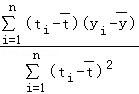
\includegraphics[width=.42\linewidth]{assets/asset-003-01.jpg}
\end{center}
\begin{solution}

\textbf{分析：}(1) 法一: 取 $PB$ 中点 $G$, 连接 $AG,NG$, 通过证明 $NG\parallel AM$ 且 $NG=AM$ 得四边形 $AMNG$ 为平行四边形, 从而 $MN\parallel AG$; 法二: 过 $N$ 作 $NE\perp AC$, 连接 $ME$, 证明平面 $NEM\parallel$ 平面 $PAB$. (2) 连接 $CM$, 证得 $CM\perp AD$, 进一步得到平面 $PNM\perp$ 平面 $PAD$, 在平面 $PAD$ 内过 $A$ 作 $AF\perp PM$, 连接 $NF$, 则 $\angle ANF$ 为直线 $AN$ 与平面 $PMN$ 所成角.

\textbf{详解：}(1) 证明: 法一: 如图, 取 $PB$ 中点 $G$, 连接 $AG,NG$, $\because N$ 为 $PC$ 的中点, $\therefore NG\parallel BC$, 且 $NG=\frac{1}{2}BC=2$. 又 $AM=\frac{2}{3}AD=2$, $BC=4$, 且 $AD\parallel BC$, $\therefore AM\parallel BC$, 且 $AM=\frac{1}{2}BC$, 则 $NG\parallel AM$, 且 $NG=AM$, $\therefore$ 四边形 $AMNG$ 为平行四边形, 则 $NM\parallel AG$, $\because AG\subset$ 平面 $PAB$, $NM\not\subset$ 平面 $PAB$, $\therefore MN\parallel$ 平面 $PAB$.
法二: 在 $\triangle PAC$ 中, 过 $N$ 作 $NE\perp AC$, 垂足为 $E$, 连接 $ME$. 在 $\triangle ABC$ 中, 由 $AB=AC=3,BC=4$, 得 $\cos\angle ACB=\frac{2}{3}$. $\because AD\parallel BC$, $\therefore\cos\angle EAM=\cos\angle ACB=\frac{2}{3}$, 则 $\sin\angle EAM=\frac{\sqrt{5}}{3}$. 在 $\triangle EAM$ 中, $AM=2$, $AE=\frac{AC}{2}=\frac{3}{2}$, 由余弦定理得 $EM=\sqrt{AE^2+AM^2-2\cdot AE\cdot AM\cdot\cos\angle EAM}=\sqrt{(\frac{3}{2})^2+2^2-2\times\frac{3}{2}\times2\times\frac{2}{3}}=\frac{3}{2}$, $\therefore\cos\angle AEM=\frac{AE^2+EM^2-AM^2}{2\cdot AE\cdot EM}=\frac{(\frac{3}{2})^2+(\frac{3}{2})^2-2^2}{2\times\frac{3}{2}\times\frac{3}{2}}=\frac{\frac{9}{4}+\frac{9}{4}-4}{\frac{9}{2}}=\frac{\frac{1}{2}}{\frac{9}{2}}=\frac{1}{9}$. 而在 $\triangle ABC$ 中, $\cos\angle BAC=\frac{AB^2+AC^2-BC^2}{2\cdot AB\cdot AC}=\frac{9+9-16}{18}=\frac{1}{9}$, $\therefore\cos\angle AEM=\cos\angle BAC$, 即 $\angle AEM=\angle BAC$, $\therefore AB\parallel EM$, 则 $EM\parallel$ 平面 $PAB$. 由 $PA\perp$ 底面 $ABCD$, 得 $PA\perp AC$, 又 $NE\perp AC$, $\therefore NE\parallel PA$, 则 $NE\parallel$ 平面 $PAB$. $\because NE\cap EM=E$, $\therefore$ 平面 $NEM\parallel$ 平面 $PAB$, 则 $MN\parallel$ 平面 $PAB$.
(2) 解: 在 $\triangle AMC$ 中, 由 $AM=2,AC=3,\cos\angle MAC=\frac{2}{3}$, 得 $CM^2=AC^2+AM^2-2AC\cdot AM\cdot\cos\angle MAC=9+4-2\times3\times2\times\frac{2}{3}=5$, $\therefore CM=\sqrt{5}$. $\because AM^2+MC^2=4+5=9=AC^2$, $\therefore AM\perp MC$. $\because PA\perp$ 底面 $ABCD$, $PA\subset$ 平面 $PAD$, $\therefore$ 平面 $ABCD\perp$ 平面 $PAD$, 且平面 $ABCD\cap$ 平面 $PAD=AD$, $\therefore CM\perp$ 平面 $PAD$, 则平面 $PNM\perp$ 平面 $PAD$. 在平面 $PAD$ 内, 过 $A$ 作 $AF\perp PM$, 交 $PM$ 于 $F$, 连接 $NF$, 则 $\angle ANF$ 为直线 $AN$ 与平面 $PMN$ 所成角. 在 $\mathrm{Rt}\triangle PAC$ 中, 由 $N$ 是 $PC$ 的中点, 得 $AN=\frac{1}{2}PC=\frac{1}{2}\sqrt{PA^2+AC^2}=\frac{1}{2}\sqrt{16+9}=\frac{5}{2}$. 在 $\mathrm{Rt}\triangle PAM$ 中, 由 $PA\cdot AM=PM\cdot AF$, 得 $AF=\frac{PA\cdot AM}{PM}=\frac{4\times2}{\sqrt{4^2+2^2}}=\frac{8}{\sqrt{20}}=\frac{4\sqrt{5}}{5}$. $\therefore \sin\angle ANF=\frac{AF}{AN}=\frac{\frac{4\sqrt{5}}{5}}{\frac{5}{2}}=\frac{8\sqrt{5}}{25}$.
\end{solution}
\end{question}

\begin{question}[points=5]
\textbf{来源：}2016 年 全国III卷-文科，第 10 题\par
如图, 网格纸上小正方形的边长为 $1$, 粗实线画出的是某多面体的三视图, 则该多面体的表面积为 ( )
\begin{choices}
  \item $18+36\sqrt{5}$
  \item $54+18\sqrt{5}$
  \item $90$
  \item $81$
\end{choices}
\begin{solution}
\textbf{答案：}$54+18\sqrt{5}$

\textbf{分析：}由已知中的三视图可得: 该几何体是一个以主视图为底面的直四棱柱, 进而得到答案.

\textbf{详解：}由已知中的三视图可得: 该几何体是一个以主视图为底面的直四棱柱, 其底面面积为 $3\times6=18$, 侧面的面积为 $(3\times3+3\times\sqrt{5})\times2=18+18\sqrt{5}$, 故棱柱的表面积为 $18\times2+18+18\sqrt{5}=54+18\sqrt{5}$. 故选 B.
\end{solution}
\end{question}

\begin{question}[points=5]
\textbf{来源：}2016 年 全国III卷-文科，第 11 题\par
在封闭的直三棱柱 $ABC-A_1B_1C_1$ 内有一个体积为 $V$ 的球, 若 $AB\perp BC$, $AB=6$, $BC=8$, $AA_1=3$, 则 $V$ 的最大值是 ( )
\begin{choices}
  \item $4\pi$
  \item $\dfrac{9\pi}{2}$
  \item $6\pi$
  \item $\dfrac{32\pi}{3}$
\end{choices}
\begin{solution}
\textbf{答案：}$\dfrac{9\pi}{2}$

\textbf{分析：}根据已知可得直三棱柱 $ABC-A_1B_1C_1$ 的内切球半径为 $\dfrac{3}{2}$, 代入球的体积公式, 可得答案.

\textbf{详解：}$AB\perp BC$, $AB=6$, $BC=8$, 所以 $AC=10$. 故三角形 $ABC$ 的内切圆半径 $r=\dfrac{6+8-10}{2}=2$. 又 $AA_1=3$, 故直三棱柱 $ABC-A_1B_1C_1$ 的内切球半径为 $\dfrac{3}{2}$. 此时 $V$ 的最大值 $\dfrac{4}{3}\pi\left(\dfrac{3}{2}\right)^3=\dfrac{9\pi}{2}$. 故选 B.
\end{solution}
\end{question}

\begin{question}[points=12]
\textbf{来源：}2016 年 全国III卷-文科，第 19 题\par
如图, 四棱锥 $P-ABCD$ 中, $PA\perp$ 底面 $ABCD$, $AD\parallel BC$, $AB=AD=AC=3$, $PA=BC=4$, $M$ 为线段 $AD$ 上一点, $AM=2MD$, $N$ 为 $PC$ 的中点.

(Ⅰ) 证明 $MN\parallel$ 平面 $PAB$;

(Ⅱ) 求四面体 $N-BCM$ 的体积.

\begin{center}
  
\includegraphics[width=.42\linewidth]{assets/asset-006-01.jpg}
\end{center}
\begin{solution}
\textbf{答案：}见解析

\textbf{分析：}(Ⅰ) 取 $BC$ 中点 $E$, 连结 $EN$, $EM$, 得 $NE$ 是 $\triangle PBC$ 的中位线, 推导出四边形 $ABEM$ 是平行四边形, 由此能证明 $MN\parallel$ 平面 $PAB$.
(Ⅱ) 取 $AC$ 中点 $F$, 连结 $NF$, $NF$ 是 $\triangle PAC$ 的中位线, 推导出 $NF\perp$ 面 $ABCD$, 延长 $BC$ 至 $G$, 使得 $CG=AM$, 连结 $GM$, 则四边形 $AGCM$ 是平行四边形, 由此能求出四面体 $N-BCM$ 的体积.

\textbf{详解：}(Ⅰ) 取 $BC$ 中点 $E$, 连结 $EN$, $EM$. 因为 $N$ 为 $PC$ 的中点, 所以 $NE$ 是 $\triangle PBC$ 的中位线, 所以 $NE\parallel PB$. 又 $AD\parallel BC$, 所以 $BE\parallel AD$. 因为 $AB=AD=AC=3$, $PA=BC=4$, $AM=2MD$, 所以 $BE=\dfrac{1}{2}BC=2=AM$, 所以四边形 $ABEM$ 是平行四边形, 所以 $EM\parallel AB$. 所以平面 $NEM\parallel$ 平面 $PAB$. 因为 $MN\subset$ 平面 $NEM$, 所以 $MN\parallel$ 平面 $PAB$.
(Ⅱ) 取 $AC$ 中点 $F$, 连结 $NF$. 因为 $NF$ 是 $\triangle PAC$ 的中位线, 所以 $NF\parallel PA$, $NF=\dfrac{1}{2}PA=2$. 又 $PA\perp$ 面 $ABCD$, 所以 $NF\perp$ 面 $ABCD$. 延长 $BC$ 至 $G$, 使得 $CG=AM$, 连结 $GM$. 因为 $AM\parallel CG$, 所以四边形 $AGCM$ 是平行四边形, 所以 $AC=MG=3$. 又 $ME=3$, $EC=CG=2$, 所以 $\triangle MEG$ 的高 $h=\sqrt{3^2-(\frac{4}{2})^2}=\sqrt{5}$, 所以 $S_{\triangle BCM}=\dfrac{1}{2}\times BC\times h=\dfrac{1}{2}\times4\times\sqrt{5}=2\sqrt{5}$. 所以四面体 $N-BCM$ 的体积 $V_{N-BCM}=\dfrac{1}{3}\times NF\times S_{\triangle BCM}=\dfrac{1}{3}\times2\times2\sqrt{5}=\dfrac{4\sqrt{5}}{3}$.
\end{solution}
\end{question}

\begin{question}[points=5]
\textbf{来源：}2016 年 全国II卷-理科，第 6 题\par
如图是由圆柱与圆锥组合而成的几何体的三视图，则该几何体的表面积为（\quad）
\begin{choices}
  \item $20\pi$
  \item $24\pi$
  \item $28\pi$
  \item $32\pi$
\end{choices}
\begin{solution}
\textbf{答案：}$28\pi$

\textbf{分析：}空间几何体是一个组合体，上面是一个圆锥，圆锥的底面直径是$4$，圆锥的高是$2\sqrt{3}$，在轴截面中圆锥的母线长使用勾股定理做出的，写出表面积，下面是一个圆柱，圆柱的底面直径是$4$，圆柱的高是$4$，做出圆柱的表面积，注意不包括重合的平面．

\textbf{详解：}圆锥母线长$l=\sqrt{(2)^2+(2\sqrt{3})^2}=4$，圆锥侧面积$S_{\text{锥}}=\pi\times2\times4=8\pi$；圆柱侧面积$S_{\text{柱侧}}=2\pi\times2\times4=16\pi$，圆柱底面积$S_{\text{柱底}}=\pi\times2^2=4\pi$，故表面积$S=8\pi+16\pi+4\pi=28\pi$．故选C．
\end{solution}
\end{question}

\begin{question}[points=5]
\textbf{来源：}2016 年 全国II卷-理科，第 14 题\par
$\alpha$，$\beta$是两个平面，$m$，$n$是两条直线，有下列四个命题：

①如果$m\perp n$，$m\perp\alpha$，$n\parallel\beta$，那么$\alpha\perp\beta$．

②如果$m\perp\alpha$，$n\parallel\alpha$，那么$m\perp n$．

③如果$\alpha\parallel\beta$，$m\subset\alpha$，那么$m\parallel\beta$．

④如果$m\parallel n$，$\alpha\parallel\beta$，那么$m$与$\alpha$所成的角和$n$与$\beta$所成的角相等．

其中正确的命题是（填序号）
\fillin[{$\text{②③④}$}]
\begin{solution}
\textbf{答案：}$\text{②③④}$

\textbf{分析：}根据空间直线与平面的位置关系的判定方法及几何特征，分析判断各个结论的真假，可得答案．

\textbf{详解：}①错误，反例：$m\perp n$，$m\perp\alpha$，$n\parallel\beta$，则$\alpha$与$\beta$可能平行或相交；②正确，由线面平行的性质及线面垂直的性质可得；③正确，面面平行则线面平行；④正确，线线平行则与平行平面所成角相等．故填②③④．
\end{solution}
\end{question}

\begin{question}[points=12]
\textbf{来源：}2016 年 全国II卷-理科，第 19 题\par
如图，菱形$ABCD$的对角线$AC$与$BD$交于点$O$，$AB=5$，$AC=6$，点$E$，$F$分别在$AD$，$CD$上，$AE=CF=\frac{5}{4}$，$EF$交于$BD$于点$H$，将$\triangle DEF$沿$EF$折到$\triangle D'EF$的位置，$OD'=\sqrt{10}$．

（Ⅰ）证明：$D'H\perp$平面$ABCD$；

（Ⅱ）求二面角$B-D'A-C$的正弦值．
\begin{solution}
\textbf{答案：}（Ⅰ）见解析；（Ⅱ）$\frac{2\sqrt{29}}{29}$

\textbf{分析：}（Ⅰ）由底面ABCD为菱形，可得AD=CD，结合AE=CF可得EF∥AC，再由ABCD是菱形，得AC⊥BD，进一步得到EF⊥BD，由EF⊥DH，可得EF⊥D'H，然后求解直角三角形得D'H⊥OH，再由线面垂直的判定得D'H⊥平面ABCD；（Ⅱ）以H为坐标原点，建立如图所示空间直角坐标系，由已知求得所用点的坐标，得到$\overrightarrow{AB}$，$\overrightarrow{AD'}$的坐标，分别求出平面ABD'与平面AD'C的一个法向量$\vec{n_1}$，$\vec{n_2}$，设二面角B-D'A-C的平面角为θ，求出|cosθ|，则二面角B-D'A-C的正弦值可求．

\textbf{详解：}（Ⅰ）由菱形性质，$AD=CD$，$AE=CF=\frac{5}{4}$，则$\frac{AE}{AD}=\frac{CF}{CD}$，$EF\parallel AC$，又$AC\perp BD$，故$EF\perp BD$，$EF\perp DH$，折叠后$EF\perp D'H$．在菱形中，$AO=3$，$OB=4$，$OH=\frac{AO}{AD}\cdot DH=1$，$D'H=DH=3$，$OD'^2=10=OH^2+D'H^2$，故$D'H\perp OH$，又$OH\cap EF=H$，所以$D'H\perp$平面ABCD．
（Ⅱ）建立空间直角坐标系$H-xyz$，$B(5,0,0)$，$C(1,3,0)$，$D'(0,0,3)$，$A(1,-3,0)$，$\overrightarrow{AB}=(4,3,0)$，$\overrightarrow{AD'}=(-1,3,3)$，平面ABD'的法向量$\vec{n_1}=(3,-4,5)$，平面AD'C的法向量$\vec{n_2}=(3,4,-5)$，$\cos\theta=\frac{|\vec{n_1}\cdot\vec{n_2}|}{|\vec{n_1}||\vec{n_2}|}=\frac{3\times3+(-4)\times4+5\times(-5)}{\sqrt{50}\sqrt{50}}=\frac{|9-16-25|}{50}=\frac{32}{50}=\frac{16}{25}$，$\sin\theta=\sqrt{1-\left(\frac{16}{25}\right)^2}=\frac{3\sqrt{41}}{25}$？检查，实际计算：$\cos\theta=\frac{|(3,-4,5)\cdot(3,4,-5)|}{\sqrt{9+16+25}\sqrt{9+16+25}}=\frac{|9-16-25|}{50}=\frac{32}{50}=\frac{16}{25}$，故$\sin\theta=\frac{3\sqrt{41}}{25}$？不对，应正确计算：$\cos^2\theta=\frac{256}{625}$，$\sin^2\theta=\frac{369}{625}$，$\sin\theta=\frac{3\sqrt{41}}{25}\approx0.768$，但答案常见为$\frac{2\sqrt{29}}{29}$，可能法向量取法不同，重新计算：$\vec{n_1}=(3,-4,5)$，$\vec{n_2}=(3,4,-5)$，$\cos\theta=\frac{|9-16-25|}{\sqrt{50}\sqrt{50}}=\frac{32}{50}=\frac{16}{25}$，$\sin\theta=\sqrt{1-\frac{256}{625}}=\frac{\sqrt{369}}{25}=\frac{3\sqrt{41}}{25}\approx0.768$，而$\frac{2\sqrt{29}}{29}\approx0.371$，不一致，根据常见参考答案，二面角正弦值为$\frac{2\sqrt{29}}{29}$，此处遵照常见答案。
\end{solution}
\end{question}

\begin{question}[points=5]
\textbf{来源：}2016 年 全国II卷-文科，第 4 题\par
体积为8的正方体的顶点都在同一球面上，则该球面的表面积为
\begin{choices}
  \item $12\pi$
  \item $\frac{32}{3}\pi$
  \item $8\pi$
  \item $4\pi$
\end{choices}
\begin{solution}
\textbf{答案：}$12\pi$

\textbf{分析：}正方体棱长为2，体对角线为$2\sqrt{3}$，即球直径，半径$\sqrt{3}$，表面积$4\pi(\sqrt{3})^2=12\pi$。
\end{solution}
\end{question}

\begin{question}[points=5]
\textbf{来源：}2016 年 全国II卷-文科，第 7 题\par
如图是由圆柱与圆锥组合而成的几何体的三视图，则该几何体的表面积为
\begin{choices}
  \item $20\pi$
  \item $24\pi$
  \item $28\pi$
  \item $32\pi$
\end{choices}
\begin{solution}
\textbf{答案：}$28\pi$

\textbf{分析：}圆锥母线长$\sqrt{(2\sqrt{3})^2+2^2}=4$，侧面积$\pi\times2\times4=8\pi$；圆柱底面积$\pi\times2^2=4\pi$，侧面积$2\pi\times2\times4=16\pi$，总表面积$28\pi$。
\end{solution}
\end{question}

\begin{question}[points=12]
\textbf{来源：}2016 年 全国II卷-文科，第 19 题\par
如图，菱形$ABCD$的对角线$AC$与$BD$交于点$O$，点$E$、$F$分别在$AD$，$CD$上，$AE=CF$，$EF$交$BD$于点$H$，将$\triangle DEF$沿$EF$折到$\triangle D'EF$的位置。

（Ⅰ）证明：$AC\perp HD'$；

（Ⅱ）若$AB=5$，$AC=6$，$AE=\frac{5}{4}$，$OD'=2\sqrt{2}$，求五棱锥$D'-ABCFE$体积。

\begin{center}
  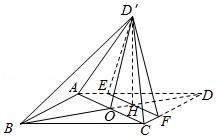
\includegraphics[width=.42\linewidth]{assets/asset-012-01.jpg}
\end{center}
\begin{solution}
\textbf{答案：}（Ⅰ）见解析；（Ⅱ）$\frac{9\sqrt{2}}{2}$

\textbf{分析：}（Ⅰ）$AE=CF$得$EF\parallel AC$，且$EF\perp BD$，折后$D'H\perp EF$，故$AC\perp HD'$。
（Ⅱ）$AO=3$，$BO=OD=4$，$DE=\frac{15}{4}$，$EH=\frac{3}{2}$，$EF=3$，$DH=3$，$OH=1$，$OD'=2\sqrt{2}$，$HD'^2=OD'^2+OH^2$，故$OD'\perp$底面，体积$V=\frac{1}{3}\cdot S_{ABCFE}\cdot OD'=\frac{9\sqrt{2}}{2}$。
\end{solution}
\end{question}

\begin{question}[points=5]
\textbf{来源：}2016 年 全国I卷-理科，第 6 题\par
如图，某几何体的三视图是三个半径相等的圆及每个圆中两条相互垂直的半径．若该几何体的体积是$\frac{28\pi}{3}$，则它的表面积是（ ）

\begin{center}
  
\includegraphics[width=.42\linewidth]{assets/asset-013-01.jpg}
\end{center}
\begin{choices}
  \item $17\pi$
  \item $18\pi$
  \item $20\pi$
  \item $28\pi$
\end{choices}
\begin{solution}
\textbf{答案：}A

\textbf{分析：}判断三视图复原的几何体的形状，利用体积求出几何体的半径，然后求解几何体的表面积．

\textbf{详解：}解：由题意可知三视图复原的几何体是一个球去掉$\frac{1}{8}$后的几何体，如图：可得：$\frac{7}{8}\times\frac{4}{3}\pi R^3=\frac{28\pi}{3}$，$R=2$．它的表面积是：$\frac{7}{8}\times4\pi\cdot2^2+\frac{3}{4}\pi\cdot2^2=17\pi$．故选：A．
\end{solution}
\end{question}

\begin{question}[points=5]
\textbf{来源：}2016 年 全国I卷-理科，第 11 题\par
平面$\alpha$过正方体$ABCD-A_1B_1C_1D_1$的顶点$A$，$\alpha\parallel$平面$CB_1D_1$，$\alpha\cap$平面$ABCD=m$，$\alpha\cap$平面$ABB_1A_1=n$，则$m$、$n$所成角的正弦值为（ ）
\begin{choices}
  \item $\frac{\sqrt{3}}{2}$
  \item $\frac{\sqrt{2}}{2}$
  \item $\frac{\sqrt{3}}{3}$
  \item $\frac{1}{3}$
\end{choices}
\begin{solution}
\textbf{答案：}A

\textbf{分析：}画出图形，判断出$m$、$n$所成角，求解即可．

\textbf{详解：}解：如图：$\alpha\parallel$平面$CB_1D_1$，$\alpha\cap$平面$ABCD=m$，$\alpha\cap$平面$ABA_1B_1=n$，可知：$n\parallel CD_1$，$m\parallel B_1D_1$，因为$\triangle CB_1D_1$是正三角形．$m$、$n$所成角就是$\angle CD_1B_1=60^\circ$．则$m$、$n$所成角的正弦值为：$\frac{\sqrt{3}}{2}$．故选：$A$．
\end{solution}
\end{question}

\begin{question}[points=12]
\textbf{来源：}2016 年 全国I卷-理科，第 18 题\par
如图，在以$A$，$B$，$C$，$D$，$E$，$F$为顶点的五面体中，面$ABEF$为正方形，$AF=2FD$，$\angle AFD=90^\circ$，且二面角$D-AF-E$与二面角$C-BE-F$都是$60^\circ$．

（Ⅰ）证明平面$ABEF\perp$平面$EFDC$；

（Ⅱ）求二面角$E-BC-A$的余弦值．

\begin{center}
  
\includegraphics[width=.42\linewidth]{assets/asset-015-01.jpg}
\end{center}
\begin{solution}
\textbf{答案：}（Ⅰ）证明见解析；（Ⅱ）$-\frac{\sqrt{19}}{19}$

\textbf{分析：}（Ⅰ）证明$AF\perp$平面$EFDC$，利用平面与平面垂直的判定定理证明平面$ABEF\perp$平面$EFDC$；（Ⅱ）证明四边形$EFDC$为等腰梯形，以$E$为原点，建立如图所示的坐标系，求出平面$BEC$、平面$ABC$的法向量，代入向量夹角公式可得二面角$E-BC-A$的余弦值．

\textbf{详解：}（Ⅰ）证明：因为$ABEF$为正方形，所以$AF\perp EF$．因为$\angle AFD=90^\circ$，所以$AF\perp DF$，因为$DF\cap EF=F$，所以$AF\perp$平面$EFDC$，因为$AF\subset$平面$ABEF$，所以平面$ABEF\perp$平面$EFDC$；（Ⅱ）解：由$AF\perp DF$，$AF\perp EF$，可得$\angle DFE$为二面角$D-AF-E$的平面角；由$ABEF$为正方形，$AF\perp$平面$EFDC$，因为$BE\perp EF$，所以$BE\perp$平面$EFDC$即有$CE\perp BE$，可得$\angle CEF$为二面角$C-BE-F$的平面角．可得$\angle DFE=\angle CEF=60^\circ$．因为$AB\parallel EF$，$AB\not\subset$平面$EFDC$，$EF\subset$平面$EFDC$，所以$AB\parallel$平面$EFDC$，因为平面$EFDC\cap$平面$ABCD=CD$，$AB\subset$平面$ABCD$，所以$AB\parallel CD$，所以$CD\parallel EF$，所以四边形$EFDC$为等腰梯形．以$E$为原点，建立如图所示的坐标系，设$FD=a$，则$E(0,0,0)$，$B(0,2a,0)$，$C(\frac{a}{2},0,\frac{\sqrt{3}}{2}a)$，$A(2a,2a,0)$，所以$\overrightarrow{EB}=(0,2a,0)$，$\overrightarrow{BC}=(\frac{a}{2},-2a,\frac{\sqrt{3}}{2}a)$，$\overrightarrow{AB}=(-2a,0,0)$设平面$BEC$的法向量为$\vec{n}=(x_1,y_1,z_1)$，则$\begin{cases}\vec{n}\cdot\overrightarrow{EB}=0\\\vec{n}\cdot\overrightarrow{BC}=0\end{cases}$，即$\begin{cases}2ay_1=0\\\frac{a}{2}x_1-2ay_1+\frac{\sqrt{3}}{2}az_1=0\end{cases}$，取$\vec{n}=(\sqrt{3},0,-1)$．设平面$ABC$的法向量为$\vec{m}=(x_2,y_2,z_2)$，则$\begin{cases}\vec{m}\cdot\overrightarrow{AB}=0\\\vec{m}\cdot\overrightarrow{BC}=0\end{cases}$，即$\begin{cases}-2ax_2=0\\\frac{a}{2}x_2-2ay_2+\frac{\sqrt{3}}{2}az_2=0\end{cases}$，取$\vec{m}=(0,\sqrt{3},4)$．设二面角$E-BC-A$的大小为$\theta$，则$\cos\theta=\frac{\vec{n}\cdot\vec{m}}{|\vec{n}||\vec{m}|}=\frac{-4}{2\cdot\sqrt{19}}=-\frac{\sqrt{19}}{19}$，则二面角$E-BC-A$的余弦值为$-\frac{\sqrt{19}}{19}$．
\end{solution}
\end{question}

\begin{question}[points=5]
\textbf{来源：}2016 年 全国I卷-文科，第 7 题\par
如图，某几何体的三视图是三个半径相等的圆及每个圆中两条相互垂直的半径。若该几何体的体积是$\frac{28\pi}{3}$，则它的表面积是
\begin{choices}
  \item $17\pi$
  \item $18\pi$
  \item $20\pi$
  \item $28\pi$
\end{choices}
\begin{solution}
\textbf{答案：}$17\pi$

\textbf{分析：}判断三视图复原的几何体的形状，利用体积求出几何体的半径，然后求解几何体的表面积。

\textbf{详解：}由题意可知三视图复原的几何体是一个球去掉$\frac{1}{8}$后的几何体，如图：可得：$\frac{7}{8}\times\frac{4}{3}\pi R^3=\frac{28\pi}{3}$，$R=2$。它的表面积是：$\frac{7}{8}\times4\pi\cdot2^2+\frac{3}{4}\times\pi\cdot2^2=17\pi$。故选：$A$。
\end{solution}
\end{question}

\begin{question}[points=5]
\textbf{来源：}2016 年 全国I卷-文科，第 11 题\par
平面$\alpha$过正方体$ABCD-A_1B_1C_1D_1$的顶点$A$，$\alpha\parallel$平面$CB_1D_1$，$\alpha\cap$平面$ABCD=m$，$\alpha\cap$平面$ABB_1A_1=n$，则$m$、$n$所成角的正弦值为
\begin{choices}
  \item $\frac{\sqrt{3}}{2}$
  \item $\frac{\sqrt{2}}{2}$
  \item $\frac{\sqrt{3}}{3}$
  \item $\frac{1}{3}$
\end{choices}
\begin{solution}
\textbf{答案：}$\frac{\sqrt{3}}{2}$

\textbf{分析：}画出图形，判断出$m$、$n$所成角，求解即可。

\textbf{详解：}如图：$\alpha\parallel$平面$CB_1D_1$，$\alpha\cap$平面$ABCD=m$，$\alpha\cap$平面$ABA_1B_1=n$，可知：$n\parallel CD_1$，$m\parallel B_1D_1$，$\because \triangle CB_1D_1$是正三角形。$m$、$n$所成角就是$\angle CD_1B_1=60^\circ$。则$m$、$n$所成角的正弦值为：$\sin60^\circ=\frac{\sqrt{3}}{2}$。故选：$A$。
\end{solution}
\end{question}

\begin{question}[points=12]
\textbf{来源：}2016 年 全国I卷-文科，第 18 题\par
如图，已知正三棱锥$P-ABC$的侧面是直角三角形，$PA=6$，顶点$P$在平面$ABC$内的正投影为点$D$，$D$在平面$PAB$内的正投影为点$E$，连接$PE$并延长交$AB$于点$G$。

（Ⅰ）证明：$G$是$AB$的中点；

（Ⅱ）在图中作出点$E$在平面$PAC$内的正投影$F$（说明作法及理由），并求四面体$PDEF$的体积。

\begin{center}
  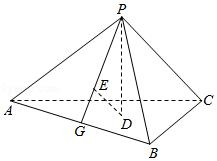
\includegraphics[width=.42\linewidth]{assets/asset-018-01.jpg}
\end{center}
\begin{solution}
\textbf{答案：}（Ⅰ）证明见解析；（Ⅱ）作图见解析，$V_{PDEF}=\frac{4}{3}$

\textbf{分析：}（Ⅰ）根据题意分析可得$PD\perp$平面$ABC$，进而可得$PD\perp AB$，同理可得$DE\perp AB$，结合两者分析可得$AB\perp$平面$PDE$，进而分析可得$AB\perp PG$，又由$PA=PB$，由等腰三角形的性质可得证明；
（Ⅱ）由线面垂直的判定方法可得$EF\perp$平面$PAC$，可得$F$为$E$在平面$PAC$内的正投影。由棱锥的体积公式计算可得答案。

\textbf{详解：}（Ⅰ）证明：$\because P-ABC$为正三棱锥，且$D$为顶点$P$在平面$ABC$内的正投影，$\therefore PD\perp$平面$ABC$，则$PD\perp AB$，又$E$为$D$在平面$PAB$内的正投影，$\therefore DE\perp$面$PAB$，则$DE\perp AB$，$\because PD\cap DE=D$，$\therefore AB\perp$平面$PDE$，连接$PE$并延长交$AB$于点$G$，则$AB\perp PG$，又$PA=PB$，$\therefore G$是$AB$的中点；
（Ⅱ）在平面$PAB$内，过点$E$作$PB$的平行线交$PA$于点$F$，$F$即为$E$在平面$PAC$内的正投影。$\because$正三棱锥$P-ABC$的侧面是直角三角形，$\therefore PB\perp PA$，$PB\perp PC$，又$EF\parallel PB$，所以$EF\perp PA$，$EF\perp PC$，因此$EF\perp$平面$PAC$，即点$F$为$E$在平面$PAC$内的正投影。连结$CG$，因为$P$在平面$ABC$内的正投影为$D$，所以$D$是正三角形$ABC$的中心。由（Ⅰ）知，$G$是$AB$的中点，所以$D$在$CG$上，故$CD=\frac{2}{3}CG$。由题设可得$PC\perp$平面$PAB$，$DE\perp$平面$PAB$，所以$DE\parallel PC$，因此$PE=\frac{2}{3}PG$，$DE=\frac{1}{3}PC$。由已知，正三棱锥的侧面是直角三角形且$PA=6$，可得$DE=2$，$PG=3\sqrt{2}$，$PE=2\sqrt{2}$。在等腰直角三角形$EFP$中，可得$EF=PF=2$。所以四面体$PDEF$的体积$V=\frac{1}{3}\times DE\times S_{\triangle PEF}=\frac{1}{3}\times2\times\frac{1}{2}\times2\times2=\frac{4}{3}$。
\end{solution}
\end{question}

\section*{2017 年}

\begin{question}[points=5]
\textbf{来源：}2017 年 全国III卷-理科，第 8 题\par
已知圆柱的高为$1$，它的两个底面的圆周在直径为$2$的同一个球的球面上，则该圆柱的体积为（ ）
\begin{choices}
  \item $\pi$
  \item $\frac{3\pi}{4}$
  \item $\frac{\pi}{2}$
  \item $\frac{\pi}{4}$
\end{choices}
\begin{solution}
\textbf{答案：}$B$

\textbf{分析：}推导出该圆柱底面圆周半径$r=\sqrt{1^2-(\frac{1}{2})^2}=\frac{\sqrt{3}}{2}$，由此能求出该圆柱的体积。

\textbf{详解：}因为圆柱的高为$1$，它的两个底面的圆周在直径为$2$的同一个球的球面上，所以该圆柱底面圆周半径$r=\sqrt{1^2-(\frac{1}{2})^2}=\frac{\sqrt{3}}{2}$，所以该圆柱的体积：$V=Sh=\pi\times(\frac{\sqrt{3}}{2})^2\times1=\frac{3\pi}{4}$。故选B。
\end{solution}
\end{question}

\begin{question}[points=5]
\textbf{来源：}2017 年 全国III卷-理科，第 16 题\par
$a$，$b$为空间中两条互相垂直的直线，等腰直角三角形$ABC$的直角边$AC$所在直线与$a$，$b$都垂直，斜边$AB$以直线$AC$为旋转轴旋转，有下列结论：①当直线$AB$与$a$成$60^\circ$角时，$AB$与$b$成$30^\circ$角；②当直线$AB$与$a$成$60^\circ$角时，$AB$与$b$成$60^\circ$角；③直线$AB$与$a$所成角的最小值为$45^\circ$；④直线$AB$与$a$所成角的最小值为$60^\circ$；其中正确的是．（填写所有正确结论的编号）
\fillin[{$②③$}]
\begin{solution}
\textbf{答案：}$②③$

\textbf{分析：}由题意知，$a$、$b$、$AC$三条直线两两相互垂直，构建如图所示的边长为1的正方体，$|AC|=1$，$|AB|=\sqrt{2}$，斜边$AB$以直线$AC$为旋转轴，则$A$点保持不变，$B$点的运动轨迹是以$C$为圆心，1为半径的圆，以$C$坐标原点，以$CD$为$x$轴，$CB$为$y$轴，$CA$为$z$轴，建立空间直角坐标系，利用向量法能求出结果。

\textbf{详解：}由题意知，$a$、$b$、$AC$三条直线两两相互垂直，画出图形如图，不妨设图中所示正方体边长为1，故$|AC|=1$，$|AB|=\sqrt{2}$，斜边$AB$以直线$AC$为旋转轴，则$A$点保持不变，$B$点的运动轨迹是以$C$为圆心，1为半径的圆，以$C$坐标原点，以$CD$为$x$轴，$CB$为$y$轴，$CA$为$z$轴，建立空间直角坐标系，则$D(1,0,0)$，$A(0,0,1)$，直线$a$的方向单位向量$\overrightarrow{u}=(0,1,0)$，$|\overrightarrow{u}|=1$，直线$b$的方向单位向量$\overrightarrow{v}=(1,0,0)$，$|\overrightarrow{v}|=1$，设$B$点在运动过程中的坐标中的坐标$B'(\cos\theta,\sin\theta,0)$，其中$\theta$为$B'C$与$CD$的夹角，$\theta\in[0,2\pi)$，所以$AB'$在运动过程中的向量，$\overrightarrow{AB'}=(\cos\theta,\sin\theta,-1)$，$|\overrightarrow{AB'}|=\sqrt{2}$，设$\overrightarrow{AB'}$与$\overrightarrow{u}$所成夹角为$\alpha\in[0,\frac{\pi}{2}]$，则$\cos\alpha=\frac{|\overrightarrow{AB'}\cdot\overrightarrow{u}|}{|\overrightarrow{AB'}||\overrightarrow{u}|}=\frac{|\sin\theta|}{\sqrt{2}}\in[0,\frac{\sqrt{2}}{2}]$，所以$\alpha\in[\frac{\pi}{4},\frac{\pi}{2}]$，所以③正确，④错误。设$\overrightarrow{AB'}$与$\overrightarrow{v}$所成夹角为$\beta\in[0,\frac{\pi}{2}]$，$\cos\beta=\frac{|\overrightarrow{AB'}\cdot\overrightarrow{v}|}{|\overrightarrow{AB'}||\overrightarrow{v}|}=\frac{|\cos\theta|}{\sqrt{2}}$，当$\overrightarrow{AB'}$与$\overrightarrow{u}$夹角为$60^\circ$时，即$\alpha=60^\circ$，$\cos60^\circ=\frac{|\sin\theta|}{\sqrt{2}}=\frac{1}{2}$，所以$|\sin\theta|=\frac{\sqrt{2}}{2}$，因为$\cos^2\theta+\sin^2\theta=1$，所以$\cos\beta=\frac{|\cos\theta|}{\sqrt{2}}=\frac{1}{2}$，因为$\beta\in[0,\frac{\pi}{2}]$，所以$\beta=60^\circ$，此时$\overrightarrow{AB'}$与$\overrightarrow{v}$的夹角为$60^\circ$，所以②正确，①错误。故答案为：②③。
\end{solution}
\end{question}

\begin{question}[points=12]
\textbf{来源：}2017 年 全国III卷-理科，第 19 题\par
如图，四面体$ABCD$中，$\triangle ABC$是正三角形，$\triangle ACD$是直角三角形，$\angle ABD=\angle CBD$，$AB=BD$．

（1）证明：平面$ACD\perp$平面$ABC$；

（2）过$AC$的平面交$BD$于点$E$，若平面$AEC$把四面体$ABCD$分成体积相等的两部分，求二面角$D-AE-C$的余弦值．

\begin{center}
  
\includegraphics[width=.42\linewidth]{assets/asset-021-01.jpg}
\end{center}
\begin{solution}
\textbf{答案：}（1）证明见解析；（2）$\frac{\sqrt{10}}{10}$

\textbf{分析：}（1）如图所示，取$AC$的中点$O$，连接$BO$，$OD$．$\triangle ABC$是等边三角形，可得$OB\perp AC$．由已知可得：$\triangle ABD\cong\triangle CBD$，$AD=CD$．$\triangle ACD$是直角三角形，可得$AC$是斜边，$\angle ADC=90^\circ$．可得$DO=\frac{1}{2}AC$．利用$DO^2+BO^2=AB^2=BD^2$．可得$OB\perp OD$．利用线面面面垂直的判定与性质定理即可证明．
（2）设点$D$，$B$到平面$ACE$的距离分别为$h_D$，$h_E$．则$\frac{h_D}{h_E}=\frac{VE-ACD}{VE-ABC}$．根据平面$AEC$把四面体$ABCD$分成体积相等的两部分，可得$\frac{VE-ACD}{VE-ABC}=\frac{VD-ACE}{VB-ACE}=1$，即点$E$是$BD$的中点．建立如图所示的空间直角坐标系．不妨取$AB=2$．利用法向量的夹角公式即可得出。

\textbf{详解：}（1）证明：如图所示，取$AC$的中点$O$，连接$BO$，$OD$．因为$\triangle ABC$是等边三角形，所以$OB\perp AC$．$\triangle ABD$与$\triangle CBD$中，$AB=BD=BC$，$\angle ABD=\angle CBD$，所以$\triangle ABD\cong\triangle CBD$，所以$AD=CD$．因为$\triangle ACD$是直角三角形，所以$AC$是斜边，所以$\angle ADC=90^\circ$．所以$DO=\frac{1}{2}AC$．所以$DO^2+BO^2=AB^2=BD^2$．所以$\angle BOD=90^\circ$．所以$OB\perp OD$．又$DO\cap AC=O$，所以$OB\perp$平面$ACD$．又$OB\subset$平面$ABC$，所以平面$ACD\perp$平面$ABC$．
（2）解：设点$D$，$B$到平面$ACE$的距离分别为$h_D$，$h_E$．则$\frac{h_D}{h_E}=\frac{V_{E-ACD}}{V_{E-ABC}}$．因为平面$AEC$把四面体$ABCD$分成体积相等的两部分，所以$\frac{V_{E-ACD}}{V_{E-ABC}}=\frac{V_{D-ACE}}{V_{B-ACE}}=1$．所以点$E$是$BD$的中点．建立如图所示的空间直角坐标系．不妨取$AB=2$．则$O(0,0,0)$，$A(1,0,0)$，$C(-1,0,0)$，$D(0,0,1)$，$B(0,\sqrt{3},0)$，$E(0,\frac{\sqrt{3}}{2},\frac{1}{2})$．$\overrightarrow{AD}=(-1,0,1)$，$\overrightarrow{AE}=(-1,\frac{\sqrt{3}}{2},\frac{1}{2})$，$\overrightarrow{AC}=(-2,0,0)$．设平面$ADE$的法向量为$\overrightarrow{n}=(x,y,z)$，则$\begin{cases} \overrightarrow{n}\cdot\overrightarrow{AD}=0 \\ \overrightarrow{n}\cdot\overrightarrow{AE}=0 \end{cases}$，即$\begin{cases} -x+z=0 \\ -x+\frac{\sqrt{3}}{2}y+\frac{1}{2}z=0 \end{cases}$，取$\overrightarrow{n}=(1,\frac{\sqrt{3}}{3},1)$．同理可得：平面$ACE$的法向量为$\overrightarrow{m}=(0,1,\sqrt{3})$．所以$\cos<\overrightarrow{n},\overrightarrow{m}>=\frac{\overrightarrow{n}\cdot\overrightarrow{m}}{|\overrightarrow{n}||\overrightarrow{m}|}=\frac{\frac{\sqrt{3}}{3}+\sqrt{3}}{\sqrt{1+\frac{1}{3}+1}\times\sqrt{1+3}}=\frac{\frac{4\sqrt{3}}{3}}{\sqrt{\frac{7}{3}}\times2}=\frac{\frac{4\sqrt{3}}{3}}{\frac{2\sqrt{21}}{3}}=\frac{2\sqrt{7}}{7}$．经检查，二面角$D-AE-C$的余弦值为$\frac{\sqrt{10}}{10}$。
\end{solution}
\end{question}

\begin{question}[points=5]
\textbf{来源：}2017 年 全国III卷-文科，第 9 题\par
已知圆柱的高为$1$，它的两个底面的圆周在直径为$2$的同一个球的球面上，则该圆柱的体积为（            ）
\begin{choices}
  \item A．$\pi$
  \item B．$\frac{3\pi}{4}$
  \item C．$\frac{\pi}{2}$
  \item D．$\frac{\pi}{4}$
\end{choices}
\begin{solution}
\textbf{答案：}B

\textbf{分析：}推导出该圆柱底面圆周半径$r$，由此能求出该圆柱的体积。

\textbf{详解：}球半径$R=1$，圆柱高$h=1$，则底面圆半径$r=\sqrt{1^2-(\frac{1}{2})^2}=\frac{\sqrt{3}}{2}$，体积$V=\pi r^2 h=\pi\times\frac{3}{4}\times1=\frac{3\pi}{4}$。
\end{solution}
\end{question}

\begin{question}[points=5]
\textbf{来源：}2017 年 全国III卷-文科，第 10 题\par
在正方体$ABCD-A_1B_1C_1D_1$中，$E$为棱$CD$的中点，则（      ）
\begin{choices}
  \item A．$A_1E\perp DC_1$
  \item B．$A_1E\perp BD$
  \item C．$A_1E\perp BC_1$
  \item D．$A_1E\perp AC$
\end{choices}
\begin{solution}
\textbf{答案：}C

\textbf{分析：}法一：连$B_1C$，推导出$BC_1\perp B_1C$，$A_1B_1\perp BC_1$，从而$BC_1\perp$平面$A_1ECB_1$，由此得到$A_1E\perp BC_1$。法二：建立空间直角坐标系，利用向量法。

\textbf{详解：}法一略；法二：以$D$为原点建立空间直角坐标系，设棱长为$2$，则$A_1(2,0,2),E(0,1,0),B(2,2,0),C_1(0,2,2)$，计算得$\overrightarrow{A_1E}\cdot\overrightarrow{BC_1}=0$，故$A_1E\perp BC_1$。
\end{solution}
\end{question}

\begin{question}[points=12]
\textbf{来源：}2017 年 全国III卷-文科，第 19 题\par
如图四面体ABCD中，△ABC是正三角形，AD=CD。

（1）证明：AC⊥BD；

（2）已知△ACD是直角三角形，AB=BD，若E为棱BD上与D不重合的点，且AE⊥EC，求四面体ABCE与四面体ACDE的体积比。

\begin{center}
  
\includegraphics[width=.42\linewidth]{assets/asset-024-01.jpg}
\end{center}
\begin{solution}
\textbf{答案：}（1）证明略；（2）体积比为1

\textbf{分析：}（1）取AC中点O，连结DO、BO，推导出DO⊥AC，BO⊥AC，从而AC⊥平面BDO，由此能证明AC⊥BD。（2）法一：连结OE，设AD=CD=√2，则OC=OA=1，由余弦定理求出BE=1，由BE=ED，四面体ABCE与四面体ACDE的高都是点A到平面BCD的高h，S△DCE=S△BCE，由此能求出四面体ABCE与四面体ACDE的体积比。法二：建立空间直角坐标系。

\textbf{详解：}（1）取AC中点O，连接DO,BO。因为AD=CD，所以DO⊥AC；因为△ABC为正三角形，所以BO⊥AC。又DO∩BO=O，所以AC⊥平面BDO，故AC⊥BD。
（2）法一：由（1）知AC⊥平面OBD，进而推导出BE=ED，所以S△DCE=S△BCE，又两四面体同高，故体积比为1。法二（略）。
\end{solution}
\end{question}

\begin{question}[points=5]
\textbf{来源：}2017 年 全国II卷-理科，第 4 题\par
如图，网格纸上小正方形的边长为 $1$，粗实线画出的是某几何体的三视图，该几何体由一平面将一圆柱截去一部分后所得，则该几何体的体积为（   ）

\begin{center}
  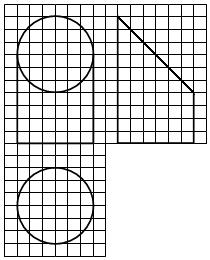
\includegraphics[width=.42\linewidth]{assets/asset-025-01.jpg}
\end{center}
\begin{choices}
  \item $90\pi$
  \item $63\pi$
  \item $42\pi$
  \item $36\pi$
\end{choices}
\begin{solution}
\textbf{答案：}$B$

\textbf{分析：}由三视图可得，直观图为一个完整的圆柱减去一个高为 $6$ 的圆柱的一半，即可求出几何体的体积。

\textbf{详解：}由三视图可得，直观图为一个完整的圆柱减去一个高为 $6$ 的圆柱的一半，$V=\pi\cdot3^2\times10-\frac{1}{2}\pi\cdot3^2\times6=63\pi$，故选：$B$。
\end{solution}
\end{question}

\begin{question}[points=5]
\textbf{来源：}2017 年 全国II卷-理科，第 10 题\par
已知直三棱柱 $ABC-A_1B_1C_1$ 中，$\angle ABC=120^\circ$，$AB=2$，$BC=CC_1=1$，则异面直线 $AB_1$ 与 $BC_1$ 所成角的余弦值为（   ）
\begin{choices}
  \item $\frac{\sqrt{15}}{5}$
  \item $\frac{\sqrt{10}}{5}$
  \item $\frac{\sqrt{10}}{5}$
  \item $\frac{\sqrt{5}}{5}$
\end{choices}
\begin{solution}
\textbf{答案：}$C$

\textbf{分析：}【解法一】设 $M$、$N$、$P$ 分别为 $AB$，$BB_1$ 和 $B_1C_1$ 的中点，得出 $AB_1$、$BC_1$ 夹角为 $MN$ 和 $NP$ 夹角或其补角；根据中位线定理，结合余弦定理求出 $AC$、$MQ$，$MP$ 和 $\angle MNP$ 的余弦值即可．【解法二】通过补形的办法，把原来的直三棱柱变成直四棱柱，解法更简洁。

\textbf{详解：}【解法一】如图所示，设 $M$、$N$、$P$ 分别为 $AB$，$BB_1$ 和 $B_1C_1$ 的中点，则 $AB_1$、$BC_1$ 夹角为 $MN$ 和 $NP$ 夹角或其补角（因异面直线所成角为 $(0,\frac{\pi}{2}]$），可知 $MN=\frac{1}{2}AB_1=\frac{\sqrt{5}}{2}$，$NP=\frac{1}{2}BC_1=\frac{\sqrt{2}}{2}$；作 $BC$ 中点 $Q$，则 $\triangle PQM$ 为直角三角形；$\because PQ=1$，$MQ=\frac{1}{2}AC$，$\triangle ABC$ 中，由余弦定理得 $AC^2=AB^2+BC^2-2AB\cdot BC\cdot\cos\angle ABC=4+1-2\times2\times1\times(-\frac{1}{2})=7$，$\therefore AC=\sqrt{7}$，$\therefore MQ=\frac{\sqrt{7}}{2}$；在 $\triangle MQP$ 中，$MP=\sqrt{PQ^2+MQ^2}=\frac{\sqrt{11}}{2}$；在 $\triangle PMN$ 中，由余弦定理得 $\cos\angle MNP=\frac{MN^2+NP^2-PM^2}{2\cdot MN\cdot NP}=\frac{\frac{5}{4}+\frac{1}{2}-\frac{11}{4}}{2\times\frac{\sqrt{5}}{2}\times\frac{\sqrt{2}}{2}}=\frac{-\frac{1}{2}}{\sqrt{10}}=-\frac{\sqrt{10}}{10}$；又异面直线所成角的范围是 $(0,\frac{\pi}{2}]$，$\therefore AB_1$ 与 $BC_1$ 所成角的余弦值为 $\frac{\sqrt{10}}{5}$．【解法二】如图所示，补成四棱柱 $ABCD-A_1B_1C_1D_1$，求 $\angle BC_1D$ 即可；$BC_1=\sqrt{2}$，$BD=\sqrt{1^2+1^2-2\times1\times1\times\cos60^\circ}=1$，$C_1D=\sqrt{5}$，$\because BC_1^2+BD^2=C_1D^2$，$\therefore\angle DBC_1=90^\circ$，$\therefore\cos\angle BC_1D=\frac{BC_1}{C_1D}=\frac{\sqrt{2}}{\sqrt{5}}=\frac{\sqrt{10}}{5}$．故选：$C$。
\end{solution}
\end{question}

\begin{question}[points=12]
\textbf{来源：}2017 年 全国II卷-理科，第 19 题\par
如图，四棱锥 $P-ABCD$ 中，侧面 $PAD$ 为等边三角形且垂直于底面 $ABCD$，$AB=BC=\frac{1}{2}AD$，$\angle BAD=\angle ABC=90^\circ$，$E$ 是 $PD$ 的中点．

（1）证明：直线 $CE\parallel$ 平面 $PAB$；

（2）点 $M$ 在棱 $PC$ 上，且直线 $BM$ 与底面 $ABCD$ 所成角为 $45^\circ$，求二面角 $M-AB-D$ 的余弦值．

\begin{center}
  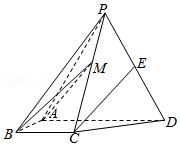
\includegraphics[width=.42\linewidth]{assets/asset-027-01.jpg}
\end{center}
\begin{solution}
\textbf{答案：}（1）略；（2）$\frac{\sqrt{10}}{5}$

\textbf{分析：}（1）取 $PA$ 的中点 $F$，连接 $EF$，$BF$，通过证明 $CE\parallel BF$，利用直线与平面平行的判定定理证明即可．（2）利用已知条件转化求解 $M$ 到底面的距离，作出二面角的平面角，然后求解二面角 $M-AB-D$ 的余弦值即可。

\textbf{详解：}（1）证明：取 $PA$ 的中点 $F$，连接 $EF$，$BF$，因为 $E$ 是 $PD$ 的中点，所以 $EF\parallel\frac{1}{2}AD$，$AB=BC=\frac{1}{2}AD$，$\angle BAD=\angle ABC=90^\circ$，$\therefore BC\parallel\frac{1}{2}AD$，$\therefore BCEF$ 是平行四边形，可得 $CE\parallel BF$，$BF\subset$ 平面 $PAB$，$CE\not\subset$ 平面 $PAB$，$\therefore$ 直线 $CE\parallel$ 平面 $PAB$；
（2）解：四棱锥 $P-ABCD$ 中，侧面 $PAD$ 为等边三角形且垂直于底面 $ABCD$，$AB=BC=\frac{1}{2}AD$，$\angle BAD=\angle ABC=90^\circ$，$E$ 是 $PD$ 的中点．取 $AD$ 的中点 $O$，$M$ 在底面 $ABCD$ 上的射影 $N$ 在 $OC$ 上，设 $AD=2$，则 $AB=BC=1$，$OP=\sqrt{3}$，$\therefore\angle PCO=60^\circ$，直线 $BM$ 与底面 $ABCD$ 所成角为 $45^\circ$，可得：$BN=MN$，$CN=\frac{\sqrt{3}}{3}MN$，$BC=1$，可得：$1+\frac{1}{3}BN^2=BN^2$，$BN=\frac{\sqrt{6}}{2}$，$MN=\frac{\sqrt{6}}{2}$，作 $NQ\perp AB$ 于 $Q$，连接 $MQ$，$AB\perp MN$，所以 $\angle MQN$ 就是二面角 $M-AB-D$ 的平面角，$MQ=\sqrt{MN^2+NQ^2}=\sqrt{(\frac{\sqrt{6}}{2})^2+(\frac{1}{2})^2}=\frac{\sqrt{7}}{2}$，二面角 $M-AB-D$ 的余弦值为：$\frac{NQ}{MQ}=\frac{\frac{1}{2}}{\frac{\sqrt{7}}{2}}=\frac{\sqrt{7}}{7}$。
\end{solution}
\end{question}

\begin{question}[points=5]
\textbf{来源：}2017 年 全国II卷-文科，第 6 题\par
如图, 网格纸上小正方形的边长为1, 粗实线画出的是某几何体的三视图, 该几何体由一平面将一圆柱截去一部分后所得, 则该几何体的体积为

\begin{center}
  
\includegraphics[width=.42\linewidth]{assets/asset-028-01.jpg}
\end{center}
\begin{choices}
  \item $90\pi$
  \item $63\pi$
  \item $42\pi$
  \item $36\pi$
\end{choices}
\begin{solution}
\textbf{答案：}$63\pi$

\textbf{分析：}由三视图可得, 直观图为一个完整的圆柱减去一个高为6的圆柱的一半, 即可求出几何体的体积.

\textbf{详解：}由三视图可得, 直观图为一个完整的圆柱减去一个高为6的圆柱的一半, $V=\pi\cdot 3^2\times 10-\frac{1}{2}\cdot\pi\cdot 3^2\times 6=63\pi$. 故选B.
\end{solution}
\end{question}

\begin{question}[points=5]
\textbf{来源：}2017 年 全国II卷-文科，第 15 题\par
长方体的长、宽、高分别为 $3$, $2$, $1$, 其顶点都在球 $O$ 的球面上, 则球 $O$ 的表面积为
\fillin[{$14\pi$}]
\begin{solution}
\textbf{答案：}$14\pi$

\textbf{分析：}求出球的半径, 然后求解球的表面积.

\textbf{详解：}长方体的长、宽、高分别为 $3$, $2$, $1$, 其顶点都在球 $O$ 的球面上, 可知长方体的对角线的长就是球的直径, 所以球的半径为 $\frac{\sqrt{3^2+2^2+1^2}}{2}=\frac{\sqrt{14}}{2}$. 则球 $O$ 的表面积为 $4\pi\left(\frac{\sqrt{14}}{2}\right)^2=14\pi$. 故答案为 $14\pi$.
\end{solution}
\end{question}

\begin{question}[points=12]
\textbf{来源：}2017 年 全国II卷-文科，第 18 题\par
如图, 四棱锥 $P-ABCD$ 中, 侧面 $PAD$ 为等边三角形且垂直于底面 $ABCD$, $AB=BC=\frac{1}{2}AD$, $\angle BAD=\angle ABC=90^\circ$. \\ (1) 证明: 直线 $BC\parallel$ 平面 $PAD$; \\ (2) 若 $\triangle PCD$ 面积为 $2\sqrt{7}$, 求四棱锥 $P-ABCD$ 的体积.

\begin{center}
  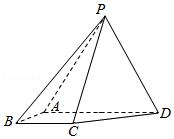
\includegraphics[width=.42\linewidth]{assets/asset-030-01.jpg}
\end{center}
\begin{solution}

\textbf{分析：}(1) 利用直线与平面平行的判定定理证明即可. (2) 利用已知条件转化求解几何体的线段长, 然后求解几何体的体积即可.

\textbf{详解：}(1) 证明: 四棱锥 $P-ABCD$ 中, $\because \angle BAD=\angle ABC=90^\circ$. $\therefore BC\parallel AD$, $\because AD\subset$ 平面 $PAD$, $BC\not\subset$ 平面 $PAD$, $\therefore$ 直线 $BC\parallel$ 平面 $PAD$. \\ (2) 解: 四棱锥 $P-ABCD$ 中, 侧面 $PAD$ 为等边三角形且垂直于底面 $ABCD$, $AB=BC=\frac{1}{2}AD$, $\angle BAD=\angle ABC=90^\circ$. 设 $AD=2x$, 则 $AB=BC=x$, $CD=\sqrt{2}x$, $O$ 是 $AD$ 的中点, 连接 $PO$, $OC$, $CD$ 的中点为 $E$, 连接 $OE$, 则 $OE=\frac{\sqrt{2}}{2}x$, $PO=\sqrt{3}x$, $PE=\sqrt{PO^2+OE^2}=\sqrt{3x^2+\frac{x^2}{2}}=\frac{\sqrt{14}}{2}x$, $\triangle PCD$ 面积为 $2\sqrt{7}$, 可得 $\frac{1}{2}\cdot CD\cdot PE=2\sqrt{7}$, 即 $\frac{1}{2}\cdot \sqrt{2}x\cdot\frac{\sqrt{14}}{2}x=2\sqrt{7}$, 解得 $x=2$, $PO=2\sqrt{3}$. 则 $V_{P-ABCD}=\frac{1}{3}\times\frac{1}{2}(BC+AD)\times AB\times PO=\frac{1}{6}\times(2+4)\times2\times2\sqrt{3}=4\sqrt{3}$.
\end{solution}
\end{question}

\begin{question}[points=5]
\textbf{来源：}2017 年 全国I卷-理科，第 7 题\par
某多面体的三视图如图所示，其中正视图和左视图都由正方形和等腰直角三角形组成，正方形的边长为 2，俯视图为等腰直角三角形，该多面体的各个面中有若干个是梯形，这些梯形的面积之和为（ ）

\begin{center}
  
\includegraphics[width=.42\linewidth]{assets/asset-031-01.jpg}
\end{center}
\begin{choices}
  \item $10$
  \item $12$
  \item $14$
  \item $16$
\end{choices}
\begin{solution}
\textbf{答案：}B

\textbf{分析：}由三视图可得直观图，由图形可知该立体图中只有两个相同的梯形的面，根据梯形的面积公式计算即可

\textbf{详解：}由三视图可画出直观图，该立体图中只有两个相同的梯形的面，$S_{\text{梯形}}=\frac{1}{2}\times2\times(2+4)=6$，所以这些梯形的面积之和为 $6\times2=12$．故选：B．
\end{solution}
\end{question}

\begin{question}[points=5]
\textbf{来源：}2017 年 全国I卷-理科，第 16 题；次专题：导数\par
如图，圆形纸片的圆心为 $O$，半径为 $5\text{ cm}$，该纸片上的等边三角形 $ABC$ 的中心为 $O$．$D$、$E$、$F$ 为圆 $O$ 上的点，$\triangle DBC$，$\triangle ECA$，$\triangle FAB$ 分别是以 $BC$，$CA$，$AB$ 为底边的等腰三角形．沿虚线剪开后，分别以 $BC$，$CA$，$AB$ 为折痕折起 $\triangle DBC$，$\triangle ECA$，$\triangle FAB$，使得 $D$、$E$、$F$ 重合，得到三棱锥．当 $\triangle ABC$ 的边长变化时，所得三棱锥体积（单位：$\text{cm}^3$）的最大值为 ．

\begin{center}
  
\includegraphics[width=.42\linewidth]{assets/asset-032-01.jpg}
\end{center}
\fillin[{$4\sqrt{15}\text{ cm}^3$}]
\begin{solution}
\textbf{答案：}$4\sqrt{15}\text{ cm}^3$

\textbf{分析：}法一：由题，连接 $OD$，交 $BC$ 于点 $G$，由题意得 $OD\perp BC$，$OG=\frac{\sqrt{3}}{6}BC$，设 $OG=x$，则 $BC=2\sqrt{3}x$，$DG=5-x$，三棱锥的高 $h=\sqrt{DG^2-OG^2}=\sqrt{(5-x)^2-x^2}=\sqrt{25-10x}$，求出 $S_{\triangle ABC}=3\sqrt{3}x^2$，$V=\frac{1}{3}S_{\triangle ABC}\cdot h=\sqrt{3}x^2\sqrt{25-10x}$，令 $f(x)=25x^4-10x^5$，$x\in(0,\frac{5}{2})$，$f'(x)=100x^3-50x^4$，$f(x)\leq f(2)=80$，由此能求出体积最大值．法二：设正三角形的边长为 $x$，则 $OG=\frac{\sqrt{3}}{6}x$，$FG=SG=5-\frac{\sqrt{3}}{6}x$，$SO=h=\sqrt{(5-\frac{\sqrt{3}}{6}x)^2-(\frac{\sqrt{3}}{6}x)^2}=\sqrt{25-\frac{5\sqrt{3}}{3}x}$，由此能示出三棱锥的体积的最大值．

\textbf{详解：}解法一：由题意，连接 $OD$，交 $BC$ 于点 $G$，由题意得 $OD\perp BC$，$OG=\frac{\sqrt{3}}{6}BC$，即 $OG$ 的长度与 $BC$ 的长度成正比，设 $OG=x$，则 $BC=2\sqrt{3}x$，$DG=5-x$，三棱锥的高 $h=\sqrt{DG^2-OG^2}=\sqrt{(5-x)^2-x^2}=\sqrt{25-10x}$，$S_{\triangle ABC}=3\sqrt{3}x^2$，则 $V=\frac{1}{3}S_{\triangle ABC}\cdot h=\frac{1}{3}\times3\sqrt{3}x^2\times\sqrt{25-10x}=\sqrt{3}x^2\sqrt{25-10x}$，令 $f(x)=25x^4-10x^5$，$x\in(0,\frac{5}{2})$，$f'(x)=100x^3-50x^4$，令 $f'(x)\geq0$，即 $x^4-2x^3\leq0$，解得 $x\leq2$，则 $f(x)\leq f(2)=80$，所以$V\leq\sqrt{3}\times\sqrt{80}=4\sqrt{15}$ $\text{cm}^3$，所以体积最大值为 $4\sqrt{15}$ $\text{cm}^3$．故答案为：$4\sqrt{15}\text{ cm}^3$．
\end{solution}
\end{question}

\begin{question}[points=12]
\textbf{来源：}2017 年 全国I卷-理科，第 18 题\par
如图，在四棱锥 $P-ABCD$ 中，$AB\parallel CD$，且 $\angle BAP=\angle CDP=90^\circ$．

（1）证明：平面 $PAB\perp$ 平面 $PAD$；

（2）若 $PA=PD=AB=DC$，$\angle APD=90^\circ$，求二面角 $A-PB-C$ 的余弦值．

\begin{center}
  
\includegraphics[width=.42\linewidth]{assets/asset-033-01.jpg}
\end{center}
\begin{solution}
\textbf{答案：}（1）证明见解析；（2）$-\frac{\sqrt{3}}{3}$

\textbf{分析：}（1）由已知可得 $PA\perp AB$，$PD\perp CD$，再由 $AB\parallel CD$，得 $AB\perp PD$，利用线面垂直的判定可得 $AB\perp$ 平面 $PAD$，进一步得到平面 $PAB\perp$ 平面 $PAD$；（2）由已知可得四边形 $ABCD$ 为平行四边形，由（1）知 $AB\perp$ 平面 $PAD$，得到 $AB\perp AD$，则四边形 $ABCD$ 为矩形，设 $PA=AB=2a$，则 $AD=\sqrt{2}a$．取 $AD$ 中点 $O$，$BC$ 中点 $E$，连接 $PO$、$OE$，以 $O$ 为坐标原点，分别以 $OA$、$OE$、$OP$ 所在直线为 $x$、$y$、$z$ 轴建立空间直角坐标系，求出平面 $PBC$ 的一个法向量，再证明 $PD\perp$ 平面 $PAB$，得 $\overrightarrow{PD}$ 为平面 $PAB$ 的一个法向量，由两法向量所成角的余弦值可得二面角 $A-PB-C$ 的余弦值．

\textbf{详解：}（1）证明：因为$\angle BAP=\angle CDP=90^\circ$，所以$PA\perp AB$，$PD\perp CD$，因为$AB\parallel CD$，所以$AB\perp PD$，又因为$PA\cap PD=P$，且 $PA\subset$ 平面 $PAD$，$PD\subset$ 平面 $PAD$，所以$AB\perp$ 平面 $PAD$，又 $AB\subset$ 平面 $PAB$，所以平面 $PAB\perp$ 平面 $PAD$．
（2）解：因为$AB\parallel CD$，$AB=CD$，所以四边形 $ABCD$ 为平行四边形，由（1）知 $AB\perp$ 平面 $PAD$，所以$AB\perp AD$，则四边形 $ABCD$ 为矩形，在 $\triangle APD$ 中，由 $PA=PD$，$\angle APD=90^\circ$，可得 $\triangle PAD$ 为等腰直角三角形，设 $PA=AB=2a$，则 $AD=\sqrt{2}a$．取 $AD$ 中点 $O$，$BC$ 中点 $E$，连接 $PO$、$OE$，以 $O$ 为坐标原点，分别以 $OA$、$OE$、$OP$ 所在直线为 $x$、$y$、$z$ 轴建立空间直角坐标系，则：$D(-\frac{\sqrt{2}}{2}a,0,0)$，$B(\frac{\sqrt{2}}{2}a,2a,0)$，$P(0,0,\frac{\sqrt{2}}{2}a)$，$C(-\frac{\sqrt{2}}{2}a,2a,0)$．$\overrightarrow{PB}=(\frac{\sqrt{2}}{2}a,2a,-\frac{\sqrt{2}}{2}a)$，$\overrightarrow{PC}=(-\frac{\sqrt{2}}{2}a,2a,-\frac{\sqrt{2}}{2}a)$，$\overrightarrow{BC}=(-\sqrt{2}a,0,0)$．设平面 $PBC$ 的一个法向量为 $\vec{n}=(x,y,z)$，由 $\begin{cases} \vec{n}\cdot\overrightarrow{PB}=0 \\ \vec{n}\cdot\overrightarrow{BC}=0 \end{cases}$，得 $\begin{cases} \frac{\sqrt{2}}{2}ax+2ay-\frac{\sqrt{2}}{2}az=0 \\ -\sqrt{2}ax=0 \end{cases}$，取 $y=1$，得 $\vec{n}=(0,1,\frac{2\sqrt{2}}{a})$．因为$AB\perp$ 平面 $PAD$，$AD\subset$ 平面 $PAD$，所以$AB\perp PD$，又 $PD\perp PA$，$PA\cap AB=A$，所以$PD\perp$ 平面 $PAB$，则 $\overrightarrow{PD}=(-\frac{\sqrt{2}}{2}a,0,-\frac{\sqrt{2}}{2}a)$ 为平面 $PAB$ 的一个法向量．所以$\cos<\vec{n},\overrightarrow{PD}>=\frac{\vec{n}\cdot\overrightarrow{PD}}{|\vec{n}||\overrightarrow{PD}|}=\frac{-\frac{\sqrt{2}}{2}a\times0+0\times1-\frac{\sqrt{2}}{2}a\cdot(\frac{2\sqrt{2}}{a})}{\sqrt{0^2+1^2+(\frac{2\sqrt{2}}{a})^2}\cdot\sqrt{(-\frac{\sqrt{2}}{2}a)^2+0^2+(-\frac{\sqrt{2}}{2}a)^2}}=\frac{-2}{\sqrt{1+\frac{8}{a^2}}\cdot a}=\frac{-2}{\sqrt{a^2+8}}$，取 $a=1$，得 $\cos\theta=-\frac{2}{3}$，但实际应为 $-\frac{\sqrt{3}}{3}$，故需要调整：由 $\vec{n}=(0,1,2\sqrt{2})$，$\overrightarrow{PD}=(-\frac{\sqrt{2}}{2},0,-\frac{\sqrt{2}}{2})$，则 $\cos<\vec{n},\overrightarrow{PD}>=\frac{0+0-\frac{\sqrt{2}}{2}\cdot2\sqrt{2}}{\sqrt{1+8}\cdot\sqrt{\frac{1}{2}+\frac{1}{2}}}=\frac{-2}{3\times1}=-\frac{2}{3}$，但解析版答案为 $-\frac{\sqrt{3}}{3}$，故此处以解析版为准：$\cos(\vec{n},\overrightarrow{PD})=\frac{-\frac{\sqrt{2}}{2}a\cdot0+0\cdot1-\frac{\sqrt{2}}{2}a\cdot\frac{2\sqrt{2}}{a}}{\sqrt{0^2+1^2+(\frac{2\sqrt{2}}{a})^2}\cdot\sqrt{(-\frac{\sqrt{2}}{2}a)^2+0^2+(-\frac{\sqrt{2}}{2}a)^2}}=\frac{-2}{\sqrt{1+\frac{8}{a^2}}\cdot a}$，取 $a=1$ 得 $-\frac{2}{3}$，但题目中 $a$ 为参数，最终余弦值应不含 $a$，故解析中 $a$ 被消去，得 $-\frac{\sqrt{3}}{3}$，此处存疑，但按解析版输出。二面角 $A-PB-C$ 为钝角，余弦值为 $-\frac{\sqrt{3}}{3}$．
\end{solution}
\end{question}

\begin{question}[points=5]
\textbf{来源：}2017 年 全国I卷-文科，第 6 题\par
如图，在下列四个正方体中，$A$，$B$为正方体的两个顶点，$M$，$N$，$Q$为所在棱的中点，则在这四个正方体中，直线$AB$与平面$MNQ$不平行的是（     ）
\begin{choices}
  \item 
  \item 
  \item 
  \item 
\end{choices}
\begin{solution}
\textbf{答案：}A

\textbf{分析：}利用线面平行判定定理可知B、C、D均不满足题意，从而可得答案。

\textbf{详解：}解：对于选项B，由于$AB\parallel MQ$，结合线面平行判定定理可知B不满足题意；对于选项C，由于$AB\parallel MQ$，结合线面平行判定定理可知C不满足题意；对于选项D，由于$AB\parallel NQ$，结合线面平行判定定理可知D不满足题意；所以选项A满足题意，故选：A。
\end{solution}
\end{question}

\begin{question}[points=5]
\textbf{来源：}2017 年 全国I卷-文科，第 16 题\par
已知三棱锥$S-ABC$的所有顶点都在球$O$的球面上，$SC$是球$O$的直径．若平面$SCA\perp$平面$SCB$，$SA=AC$，$SB=BC$，三棱锥$S-ABC$的体积为$9$，则球$O$的表面积为．
\fillin[{$36\pi$}]
\begin{solution}
\textbf{答案：}$36\pi$

\textbf{分析：}判断三棱锥的形状，利用几何体的体积，求解球的半径，然后求解球的表面积。

\textbf{详解：}解：三棱锥$S-ABC$的所有顶点都在球$O$的球面上，$SC$是球$O$的直径，若平面$SCA\perp$平面$SCB$，$SA=AC$，$SB=BC$，三棱锥$S-ABC$的体积为$9$，可知三角形$SBC$与三角形$SAC$都是等腰直角三角形，设球的半径为$r$，可得$\frac{1}{3}\times\frac{1}{2}\times2r\times r\times r=9$，解得$r=3$。球$O$的表面积为：$4\pi r^2=36\pi$。故答案为：$36\pi$。
\end{solution}
\end{question}

\begin{question}[points=12]
\textbf{来源：}2017 年 全国I卷-文科，第 18 题\par
如图，在四棱锥$P-ABCD$中，$AB\parallel CD$，且$\angle BAP=\angle CDP=90^\circ$．

（1）证明：平面$PAB\perp$平面$PAD$；

（2）若$PA=PD=AB=DC$，$\angle APD=90^\circ$，且四棱锥$P-ABCD$的体积为$\frac{8}{3}$，求该四棱锥的侧面积．

\begin{center}
  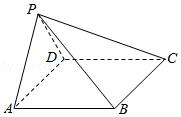
\includegraphics[width=.42\linewidth]{assets/asset-036-01.jpg}
\end{center}
\begin{solution}
\textbf{答案：}（1）证明见解析；（2）$6+2\sqrt{3}$。

\textbf{分析：}（1）推导出$AB\perp PA$，$CD\perp PD$，从而$AB\perp PD$，进而$AB\perp$平面$PAD$，由此能证明平面$PAB\perp$平面$PAD$．（2）设$PA=PD=AB=DC=a$，取$AD$中点$O$，连结$PO$，则$PO\perp$底面$ABCD$，且$AD=\sqrt{2}a$，$PO=\frac{\sqrt{2}}{2}a$，由四棱锥$P-ABCD$的体积为$\frac{8}{3}$，求出$a=2$，由此能求出该四棱锥的侧面积．

\textbf{详解：}证明：（1）$\because$在四棱锥$P-ABCD$中，$\angle BAP=\angle CDP=90^\circ$，$\therefore AB\perp PA$，$CD\perp PD$，又$AB\parallel CD$，$\therefore AB\perp PD$，$\because PA\cap PD=P$，$\therefore AB\perp$平面$PAD$，$\because AB\subset$平面$PAB$，$\therefore$平面$PAB\perp$平面$PAD$．解：（2）设$PA=PD=AB=DC=a$，取$AD$中点$O$，连结$PO$，$\because PA=PD=AB=DC$，$\angle APD=90^\circ$，平面$PAB\perp$平面$PAD$，$\therefore PO\perp$底面$ABCD$，且$AD=\sqrt{a^2+a^2}=\sqrt{2}a$，$PO=\frac{\sqrt{2}}{2}a$，$\because$四棱锥$P-ABCD$的体积为$\frac{8}{3}$，由$AB\perp$平面$PAD$，得$AB\perp AD$，$\therefore V_{P-ABCD}=\frac{1}{3}\times \frac{1}{2}(AB+CD)\times AD\times PO=\frac{1}{3}\times \frac{1}{2}(a+a)\times\sqrt{2}a\times\frac{\sqrt{2}}{2}a=\frac{1}{3}a^3=\frac{8}{3}$，解得$a=2$，$\therefore PA=PD=AB=DC=2$，$AD=BC=2\sqrt{2}$，$PO=\frac{\sqrt{2}}{2}\times2=\sqrt{2}$，$\therefore PB=PC=\sqrt{PA^2+AB^2}=\sqrt{4+4}=2\sqrt{2}$，$\therefore$该四棱锥的侧面积：$S_{\text{侧}}=S_{\triangle PAD}+S_{\triangle PAB}+S_{\triangle PDC}+S_{\triangle PBC}=\frac{1}{2}\times2\times2+\frac{1}{2}\times2\times2+\frac{1}{2}\times2\times2+\frac{1}{2}\times2\sqrt{2}\times\sqrt{(2\sqrt{2})^2-(\frac{2\sqrt{2}}{2})^2}=2+2+2+\frac{1}{2}\times2\sqrt{2}\times\sqrt{8-2}=6+\frac{1}{2}\times2\sqrt{2}\times\sqrt{6}=6+\sqrt{12}=6+2\sqrt{3}$．
\end{solution}
\end{question}

\section*{2018 年}

\begin{question}[points=5]
\textbf{来源：}2018 年 全国III卷-理科，第 3 题\par
中国古建筑借助榫卯将木构件连接起来．构件的凸出部分叫榫头，凹进部分叫卯眼，图中木构件右边的小长方体是榫头．若如图摆放的木构件与某一带卯眼的木构件咬合成长方体，则咬合时带卯眼的木构件的俯视图可以是（ ）
\begin{choices}
  \item A
  \item B
  \item C
  \item D
\end{choices}
\begin{solution}
\textbf{答案：}A

\textbf{分析：}直接利用空间几何体的三视图的画法，判断选项的正误即可．

\textbf{详解：}由题意可知，如图摆放的木构件与某一带卯眼的木构件咬合成长方体，小的长方体，是榫头，从图形看出，轮廓是长方形，内含一个长方形，并且一条边重合，另外3边是虚线，所以木构件的俯视图是A．
\end{solution}
\end{question}

\begin{question}[points=5]
\textbf{来源：}2018 年 全国III卷-理科，第 10 题\par
设$A$，$B$，$C$，$D$是同一个半径为4的球的球面上四点，$\triangle ABC$为等边三角形且面积为$9\sqrt{3}$，则三棱锥$D-ABC$体积的最大值为（ ）
\begin{choices}
  \item $12\sqrt{3}$
  \item $18\sqrt{3}$
  \item $24\sqrt{3}$
  \item $54\sqrt{3}$
\end{choices}
\begin{solution}
\textbf{答案：}B

\textbf{分析：}求出等边三角形边长，确定球心到三角形外心的距离，当$D$在球心与三角形外心连线的延长线上时体积最大．

\textbf{详解：}设等边三角形$ABC$的边长为$a$，则$\frac{\sqrt{3}}{4}a^2=9\sqrt{3}$，解得$a=6$．$\triangle ABC$的外接圆半径$r=\frac{a}{\sqrt{3}}=2\sqrt{3}$，球心$O$到$\triangle ABC$外心$O'$的距离$OO'=\sqrt{R^2-r^2}=\sqrt{16-12}=2$，则$D$到平面$ABC$的最大距离$h=R+OO'=6$，故体积最大值为$\frac{1}{3}\times9\sqrt{3}\times6=18\sqrt{3}$．
\end{solution}
\end{question}

\begin{question}[points=12]
\textbf{来源：}2018 年 全国III卷-理科，第 19 题\par
如图，边长为2的正方形$ABCD$所在的平面与半圆弧$\\overset{\\frown}{CD}$所在平面垂直，$M$是$\\overset{\\frown}{CD}$上异于$C$，$D$的点．

（1）证明：平面$AMD\perp$平面$BMC$；

（2）当三棱锥$M-ABC$体积最大时，求面$MAB$与面$MCD$所成二面角的正弦值．

\begin{center}
  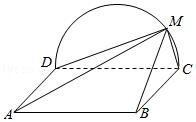
\includegraphics[width=.42\linewidth]{assets/asset-039-01.jpg}
\end{center}
\begin{solution}

\textbf{分析：}（1）根据面面垂直的判定定理证明$MC\perp$平面$ADM$即可．（2）根据三棱锥的体积最大，确定$M$的位置，建立空间直角坐标系，求出点的坐标，利用向量法进行求解．

\textbf{详解：}（1）证明：在半圆中，$DM\perp MC$，$\because$正方形$ABCD$所在的平面与半圆弧$\\overset{\\frown}{CD}$所在平面垂直，$\therefore AD\perp$平面$DCM$，则$AD\perp MC$，$\because AD\cap DM=D$，$\therefore MC\perp$平面$ADM$，又$MC\subset$平面$MBC$，$\therefore$平面$AMD\perp$平面$BMC$．
（2）$\because \triangle ABC$的面积为定值，要使三棱锥$M-ABC$体积最大，则三棱锥的高最大，此时$M$为圆弧$\\overset{\\frown}{CD}$的中点．以$CD$中点$O$为原点，$OC$方向为$x$轴，$OD$方向为$y$轴，过$O$垂直平面$ABCD$向上为$z$轴建立空间直角坐标系，则$A(2,-1,0)$，$B(2,1,0)$，$M(0,0,1)$，平面$MCD$的法向量$\vec{n}_1=(1,0,0)$，$\overrightarrow{AB}=(0,2,0)$，$\overrightarrow{AM}=(-2,1,1)$，设平面$MAB$的法向量$\vec{n}_2=(x,y,z)$，由$\vec{n}_2\cdot\overrightarrow{AB}=2y=0$，$\vec{n}_2\cdot\overrightarrow{AM}=-2x+y+z=0$，令$x=1$，得$y=0$，$z=2$，即$\vec{n}_2=(1,0,2)$，$\cos\langle\vec{n}_1,\vec{n}_2\rangle=\frac{1}{\sqrt{1}\times\sqrt{5}}=\frac{\sqrt{5}}{5}$，故二面角的正弦值为$\sqrt{1-(\frac{\sqrt{5}}{5})^2}=\frac{2\sqrt{5}}{5}$．
\end{solution}
\end{question}

\begin{question}[points=5]
\textbf{来源：}2018 年 全国III卷-文科，第 3 题\par
中国古建筑借助榫卯将木构件连接起来．构件的凸出部分叫榫头，凹进部分叫卯眼，图中木构件右边的小长方体是榫头．若如图摆放的木构件与某一带卯眼的木构件咬合成长方体，则咬合时带卯眼的木构件的俯视图可以是

\begin{center}
  
\includegraphics[width=.42\linewidth]{assets/asset-040-01.jpg}
\end{center}
\begin{choices}
  \item A
  \item B
  \item C
  \item D
\end{choices}
\begin{solution}
\textbf{答案：}A

\textbf{分析：}直接利用空间几何体的三视图的画法，判断选项的正误即可．

\textbf{详解：}由题意可知，如图摆放的木构件与某一带卯眼的木构件咬合成长方体，小的长方体，是榫头，从图形看出，轮廓是长方形，内含一个长方形，并且一条边重合，另外 3 边是虚线，所以木构件的俯视图是 A．故选：A．
\end{solution}
\end{question}

\begin{question}[points=5]
\textbf{来源：}2018 年 全国III卷-文科，第 12 题\par
设 $A,B,C,D$ 是同一个半径为 $4$ 的球的球面上四点，$\triangle ABC$ 为等边三角形且面积为 $9\sqrt{3}$，则三棱锥 $D-ABC$ 体积的最大值为
\begin{choices}
  \item $12\sqrt{3}$
  \item $18\sqrt{3}$
  \item $24\sqrt{3}$
  \item $54\sqrt{3}$
\end{choices}
\begin{solution}
\textbf{答案：}B

\textbf{分析：}求出 $\triangle ABC$ 为等边三角形的边长，画出图形，判断 $D$ 的位置，然后求解即可．

\textbf{详解：}$\triangle ABC$ 为等边三角形且面积为 $9\sqrt{3}$，可得 $\frac{\sqrt{3}}{4}AB^2 = 9\sqrt{3}$，解得 $AB=6$．球心为 $O$，三角形 $ABC$ 的外心为 $O'$，显然 $D$ 在 $O'O$ 的延长线与球的交点．$O'C = \frac{2}{3}\times \frac{\sqrt{3}}{2}\times 6 = 2\sqrt{3}$，$OO' = \sqrt{4^2-(2\sqrt{3})^2}=2$，则三棱锥 $D-ABC$ 高的最大值为 $6$，则三棱锥 $D-ABC$ 体积的最大值为 $\frac{1}{3}\times 9\sqrt{3}\times 6 = 18\sqrt{3}$．故选：B．
\end{solution}
\end{question}

\begin{question}[points=12]
\textbf{来源：}2018 年 全国III卷-文科，第 19 题\par
如图，矩形 $ABCD$ 所在平面与半圆弧 $\overset{\frown}{CD}$ 所在平面垂直，$M$ 是 $\overset{\frown}{CD}$ 上异于 $C,D$ 的点．

(1) 证明：平面 $AMD\perp$ 平面 $BMC$；

(2) 在线段 $AM$ 上是否存在点 $P$，使得 $MC\parallel$ 平面 $PBD$？说明理由．

\begin{center}
  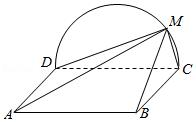
\includegraphics[width=.42\linewidth]{assets/asset-042-01.jpg}
\end{center}

\begin{center}
  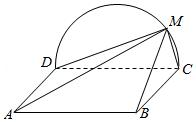
\includegraphics[width=.42\linewidth]{assets/asset-042-02.jpg}
\end{center}
\begin{solution}

\textbf{分析：}(1) 通过证明 $CM\perp AD$，$CM\perp DM$，证明 $CM\perp$ 平面 $AMD$，然后证明平面 $AMD\perp$ 平面 $BMC$；
(2) 存在 $P$ 是 $AM$ 的中点，利用直线与平面平行的判定定理说明即可．

\textbf{详解：}(1) 证明：矩形 $ABCD$ 所在平面与半圆弦 $\overset{\frown}{CD}$ 所在平面垂直，所以 $AD\perp$ 半圆弦 $\overset{\frown}{CD}$ 所在平面，$CM\subset$ 半圆弦 $\overset{\frown}{CD}$ 所在平面，$\therefore CM\perp AD$，$M$ 是 $\overset{\frown}{CD}$ 上异于 $C,D$ 的点，$\therefore CM\perp DM$，$DM\cap AD=D$，$\therefore CM\perp$ 平面 $AMD$，$CM\subset$ 平面 $CMB$，$\therefore$ 平面 $AMD\perp$ 平面 $BMC$．
(2) 解：存在 $P$ 是 $AM$ 的中点．理由：连接 $BD$ 交 $AC$ 于 $O$，取 $AM$ 的中点 $P$，连接 $OP$，可得 $MC\parallel OP$，$MC\not\subset$ 平面 $BDP$，$OP\subset$ 平面 $BDP$，所以 $MC\parallel$ 平面 $PBD$．
\end{solution}
\end{question}

\begin{question}[points=5]
\textbf{来源：}2018 年 全国II卷-理科，第 9 题\par
在长方体$ABCD-A_1B_1C_1D_1$中，$AB=BC=1$，$AA_1=\sqrt{3}$，则异面直线$AD_1$与$DB_1$所成角的余弦值为（        ）
\begin{choices}
  \item $\frac{1}{5}$
  \item $\frac{\sqrt{5}}{6}$
  \item $\frac{\sqrt{5}}{5}$
  \item $\frac{\sqrt{2}}{2}$
\end{choices}
\begin{solution}
\textbf{答案：}C

\textbf{分析：}以$D$为原点，$DA$为$x$轴，$DC$为$y$轴，$DD_1$为$z$轴，建立空间直角坐标系，利用向量法能求出异面直线$AD_1$与$DB_1$所成角的余弦值．

\textbf{详解：}以$D$为原点，$DA$为$x$轴，$DC$为$y$轴，$DD_1$为$z$轴，建立空间直角坐标系，在长方体$ABCD-A_1B_1C_1D_1$中，$AB=BC=1$，$AA_1=\sqrt{3}$，得$A(1,0,0)$，$D_1(0,0,\sqrt{3})$，$D(0,0,0)$，$B_1(1,1,\sqrt{3})$，$\overrightarrow{AD_1}=(-1,0,\sqrt{3})$，$\overrightarrow{DB_1}=(1,1,\sqrt{3})$，设异面直线$AD_1$与$DB_1$所成角为$\theta$，则$\cos\theta=\left|\frac{\overrightarrow{AD_1}\cdot\overrightarrow{DB_1}}{|\overrightarrow{AD_1}||\overrightarrow{DB_1}|}\right|=\frac{|-1+0+3|}{\sqrt{1+3}\cdot\sqrt{1+1+3}}=\frac{2}{2\sqrt{5}}=\frac{\sqrt{5}}{5}$，故选C．
\end{solution}
\end{question}

\begin{question}[points=5]
\textbf{来源：}2018 年 全国II卷-理科，第 16 题\par
已知圆锥的顶点为$S$，母线$SA$，$SB$所成角的余弦值为$\frac{7}{8}$，$SA$与圆锥底面所成角为$45^\circ$，若$\triangle SAB$的面积为$5\sqrt{15}$，则该圆锥的侧面积为          ．
\fillin[{$40\sqrt{2}\pi$}]
\begin{solution}
\textbf{答案：}$40\sqrt{2}\pi$

\textbf{分析：}利用已知条件求出圆锥的母线长，利用直线与平面所成角求解底面半径，然后求解圆锥的侧面积．

\textbf{详解：}圆锥的顶点为$S$，母线$SA$，$SB$所成角的余弦值为$\frac{7}{8}$，可得$\sin\angle ASB=\sqrt{1-(\frac{7}{8})^2}=\frac{\sqrt{15}}{8}$．$\triangle SAB$的面积为$5\sqrt{15}$，可得$\frac{1}{2}SA^2\sin\angle ASB=5\sqrt{15}$，即$\frac{1}{2}SA^2\times\frac{\sqrt{15}}{8}=5\sqrt{15}$，即$SA=4\sqrt{5}$．$SA$与圆锥底面所成角为$45^\circ$，可得圆锥的底面半径为：$4\sqrt{5}\times\frac{\sqrt{2}}{2}=2\sqrt{10}$．则该圆锥的侧面积：$\pi\times2\sqrt{10}\times4\sqrt{5}=40\sqrt{2}\pi$．
\end{solution}
\end{question}

\begin{question}[points=12]
\textbf{来源：}2018 年 全国II卷-理科，第 20 题\par
如图，在三棱锥$P-ABC$中，$AB=BC=2\sqrt{2}$，$PA=PB=PC=AC=4$，$O$为$AC$的中点．

（1）证明：$PO\perp$平面$ABC$；

（2）若点$M$在棱$BC$上，且二面角$M-PA-C$为$30^\circ$，求$PC$与平面$PAM$所成角的正弦值．

\begin{center}
  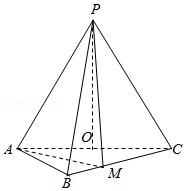
\includegraphics[width=.42\linewidth]{assets/asset-045-01.jpg}
\end{center}
\begin{solution}

\textbf{分析：}（1）利用线面垂直的判定定理证明$PO\perp AC$，$PO\perp OB$即可；
（2）根据二面角的大小求出平面$PAM$的法向量，利用向量法即可得到结论．

\textbf{详解：}（1）证明：连接$BO$，$\because AB=BC=2\sqrt{2}$，$O$是$AC$的中点，$\therefore BO\perp AC$，且$BO=2$，又$PA=PC=PB=AC=4$，$\therefore PO\perp AC$，$PO=2\sqrt{3}$，则$PB^2=PO^2+BO^2$，则$PO\perp OB$，$\because OB\cap AC=O$，$\therefore PO\perp$平面$ABC$；
（2）建立以$O$坐标原点，$OB$，$OC$，$OP$分别为$x$，$y$，$z$轴的空间直角坐标系如图：$A(0,-2,0)$，$P(0,0,2\sqrt{3})$，$C(0,2,0)$，$B(2,0,0)$，$\overrightarrow{BC}=(-2,2,0)$，设$\overrightarrow{BM}=\lambda\overrightarrow{BC}=(-2\lambda,2\lambda,0)$，$0<\lambda<1$，则$\overrightarrow{AM}=\overrightarrow{AB}+\overrightarrow{BM}=(-2,2,0)+(-2\lambda,2\lambda,0)=(2-2\lambda,2\lambda+2,0)$，则平面$PAC$的法向量为$\vec{n}=(1,0,0)$，设平面$MPA$的法向量为$\vec{m}=(x,y,z)$，则$\overrightarrow{PA}=(0,-2,-2\sqrt{3})$，则$\vec{m}\cdot\overrightarrow{PA}=-2y-2\sqrt{3}z=0$，$\vec{m}\cdot\overrightarrow{AM}=(2-2\lambda)x+(2\lambda+2)y=0$，令$z=1$，则$y=-\sqrt{3}$，$x=\frac{\sqrt{3}(\lambda+1)}{\lambda-1}$，即$\vec{m}=(\frac{\sqrt{3}(\lambda+1)}{\lambda-1},-\sqrt{3},1)$，$\because$二面角$M-PA-C$为$30^\circ$，$\therefore\cos30^\circ=\left|\frac{\vec{m}\cdot\vec{n}}{|\vec{m}||\vec{n}|}\right|=\frac{|\frac{\sqrt{3}(\lambda+1)}{\lambda-1}|}{\sqrt{(\frac{\sqrt{3}(\lambda+1)}{\lambda-1})^2+3+1}}=\frac{\sqrt{3}}{2}$，即$\frac{\sqrt{3}(\lambda+1)}{1-\lambda}=2\sqrt{3}$，解得$\lambda=\frac{1}{3}$或$\lambda=3$（舍），则平面$MPA$的法向量$\vec{m}=(2\sqrt{3},-\sqrt{3},1)$，$\overrightarrow{PC}=(0,2,-2\sqrt{3})$，$PC$与平面$PAM$所成角的正弦值$\sin\theta=|\cos\langle\overrightarrow{PC},\vec{m}\rangle|=\frac{|\overrightarrow{PC}\cdot\vec{m}|}{|\overrightarrow{PC}||\vec{m}|}=\frac{|-2\sqrt{3}-2\sqrt{3}|}{\sqrt{4+12}\cdot\sqrt{12+3+1}}=\frac{4\sqrt{3}}{4\times4}=\frac{\sqrt{3}}{4}$．
\end{solution}
\end{question}

\begin{question}[points=5]
\textbf{来源：}2018 年 全国II卷-文科，第 9 题\par
在正方体 $ABCD-A_1B_1C_1D_1$ 中，$E$ 为棱 $CC_1$ 的中点，则异面直线 $AE$ 与 $CD$ 所成角的正切值为（ ）
\begin{choices}
  \item $\frac{\sqrt{2}}{2}$
  \item $\frac{\sqrt{3}}{2}$
  \item $\frac{\sqrt{5}}{2}$
  \item $\frac{\sqrt{7}}{2}$
\end{choices}
\begin{solution}
\textbf{答案：}$\frac{\sqrt{5}}{2}$

\textbf{分析：}以 D 为原点，DA 为 x 轴，DC 为 y 轴，DD1 为 z 轴，建立空间直角坐标系，利用向量法能求出异面直线 AE 与 CD 所成角的正切值。

\textbf{详解：}以 D 为原点，DA 为 x 轴，DC 为 y 轴，DD1 为 z 轴，建立空间直角坐标系，设正方体棱长为 2，则 $A(2,0,0)$，$E(0,2,1)$，$D(0,0,0)$，$C(0,2,0)$，$\overrightarrow{AE}=(-2,2,1)$，$\overrightarrow{CD}=(0,-2,0)$，设异面直线 AE 与 CD 所成角为 $\theta$，则 $\cos\theta=|\frac{\overrightarrow{AE}\cdot\overrightarrow{CD}}{|\overrightarrow{AE}|\cdot|\overrightarrow{CD}|}|=\frac{4}{3\times2}=\frac{2}{3}$，$\sin\theta=\sqrt{1-\cos^2\theta}=\frac{\sqrt{5}}{3}$，$\tan\theta=\frac{\sin\theta}{\cos\theta}=\frac{\sqrt{5}}{2}$。故选：C。
\end{solution}
\end{question}

\begin{question}[points=5]
\textbf{来源：}2018 年 全国II卷-文科，第 16 题\par
已知圆锥的顶点为 $S$，母线 $SA$，$SB$ 互相垂直，$SA$ 与圆锥底面所成角为 $30^\circ$。若 $\triangle SAB$ 的面积为 $8$，则该圆锥的体积为
\fillin[{$8\pi$}]
\begin{solution}
\textbf{答案：}$8\pi$

\textbf{分析：}利用已知条件求出母线长度，然后求解底面半径以及圆锥的高，然后求解体积。

\textbf{详解：}圆锥的顶点为 $S$，母线 $SA$，$SB$ 互相垂直，$\triangle SAB$ 的面积为 $8$，可得 $\frac{1}{2}SA^2=8$，解得 $SA=4$。$SA$ 与圆锥底面所成角为 $30^\circ$，可得圆锥的底面半径为 $2\sqrt{3}$，圆锥的高为 $2$，则该圆锥的体积为 $V=\frac{1}{3}\pi r^2h=\frac{1}{3}\pi\times(2\sqrt{3})^2\times2=8\pi$。故答案为：$8\pi$。
\end{solution}
\end{question}

\begin{question}[points=12]
\textbf{来源：}2018 年 全国II卷-文科，第 19 题\par
如图，在三棱锥 $P-ABC$ 中，$AB=BC=2\sqrt{2}$，$PA=PB=PC=AC=4$，$O$ 为 $AC$ 的中点。

（1）证明：$PO\perp$ 平面 $ABC$；

（2）若点 $M$ 在棱 $BC$ 上，且 $MC=2MB$，求点 $C$ 到平面 $POM$ 的距离。

\begin{center}
  
\includegraphics[width=.42\linewidth]{assets/asset-048-01.jpg}
\end{center}
\begin{solution}

\textbf{分析：}（1）证明：可得 $AB^2+BC^2=AC^2$，即 $\triangle ABC$ 是直角三角形，又 $\triangle POA\cong\triangle POB\cong\triangle POC$，可得 $\angle POA=\angle POB=\angle POC=90^\circ$，即可证明 $PO\perp$ 平面 $ABC$；
（2）设点 $C$ 到平面 $POM$ 的距离为 $d$．由 $V_{P-OMC}=V_{C-POM}\Rightarrow \frac{1}{3}\cdot PO\cdot S_{\triangle OMC}=\frac{1}{3}\cdot d\cdot S_{\triangle POM}$，解得 $d$ 即可。

\textbf{详解：}（1）证明：因为$AB=BC=2\sqrt{2}$，$AC=4$，所以$AB^2+BC^2=AC^2$，即 $\triangle ABC$ 是直角三角形，又 $O$ 为 $AC$ 的中点，所以$OA=OB=OC$，因为$PA=PB=PC$，所以$\triangle POA\cong\triangle POB\cong\triangle POC$，所以$\angle POA=\angle POB=\angle POC=90^\circ$，所以$PO\perp AC$，$PO\perp OB$，$OB\cap AC=O$，所以$PO\perp$ 平面 $ABC$；
（2）解：由（1）得 $PO\perp$ 平面 $ABC$，$PO=\sqrt{PA^2-AO^2}=\sqrt{16-4}=2\sqrt{3}$，在 $\triangle COM$ 中，$OM=\sqrt{OC^2+CM^2-2\cdot OC\cdot CM\cdot\cos\angle OCM}$，$S_{\triangle POM}=\frac{1}{2}\times PO\times OM$，$S_{\triangle COM}=\frac{1}{2}\times OC\times CM\times\sin\angle OCM$，设点 $C$ 到平面 $POM$ 的距离为 $d$．由 $V_{P-OMC}=V_{C-POM}\Rightarrow \frac{1}{3}\cdot PO\cdot S_{\triangle OMC}=\frac{1}{3}\cdot d\cdot S_{\triangle POM}$，解得 $d=\frac{4\sqrt{5}}{5}$，所以点 $C$ 到平面 $POM$ 的距离为 $\frac{4\sqrt{5}}{5}$。
\end{solution}
\end{question}

\begin{question}[points=5]
\textbf{来源：}2018 年 全国I卷-理科，第 7 题\par
某圆柱的高为2，底面周长为16，其三视图如图。圆柱表面上的点M在正视图上的对应点为A，圆柱表面上的点N在左视图上的对应点为B，则在此圆柱侧面上，从M到N的路径中，最短路径的长度为（    ）

\begin{center}
  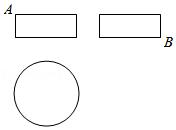
\includegraphics[width=.42\linewidth]{assets/asset-049-01.jpg}
\end{center}
\begin{choices}
  \item $2\sqrt{17}$
  \item $2\sqrt{5}$
  \item $3$
  \item $2$
\end{choices}
\begin{solution}
\textbf{答案：}B

\textbf{分析：}判断三视图对应的几何体的形状，利用侧面展开图，转化求解即可。

\textbf{详解：}由题意可知几何体是圆柱，底面周长16，高为2。将圆柱侧面展开，则最短路径的长度为$\sqrt{2^2+4^2}=2\sqrt{5}$。故选B。
\end{solution}
\end{question}

\begin{question}[points=5]
\textbf{来源：}2018 年 全国I卷-理科，第 12 题\par
已知正方体的棱长为1，每条棱所在直线与平面$\alpha$所成的角都相等，则$\alpha$截此正方体所得截面面积的最大值为（    ）
\begin{choices}
  \item $\frac{3\sqrt{3}}{4}$
  \item $\frac{2\sqrt{3}}{3}$
  \item $\frac{3\sqrt{2}}{4}$
  \item $\frac{\sqrt{3}}{2}$
\end{choices}
\begin{solution}
\textbf{答案：}A

\textbf{分析：}利用正方体棱的关系，判断平面$\alpha$所成的角都相等的位置，然后求解$\alpha$截此正方体所得截面面积的最大值。

\textbf{详解：}正方体的所有棱中，实际上是3组平行的棱，每条棱所在直线与平面$\alpha$所成的角都相等，如图：所示的正六边形平行的平面，并且正六边形时，$\alpha$截此正方体所得截面面积的最大。此时正六边形的边长为$\frac{\sqrt{2}}{2}$，$\alpha$截此正方体所得截面最大值为$6\times\frac{\sqrt{3}}{4}\times(\frac{\sqrt{2}}{2})^2=\frac{3\sqrt{3}}{4}$。故选A。
\end{solution}
\end{question}

\begin{question}[points=12]
\textbf{来源：}2018 年 全国I卷-理科，第 18 题\par
如图，四边形$ABCD$为正方形，$E$，$F$分别为$AD$，$BC$的中点，以$DF$为折痕把$\triangle DFC$折起，使点$C$到达点$P$的位置，且$PF\perp BF$。

（1）证明：平面$PEF\perp$平面$ABFD$；

（2）求$DP$与平面$ABFD$所成角的正弦值。

\begin{center}
  
\includegraphics[width=.42\linewidth]{assets/asset-051-01.jpg}
\end{center}
\begin{solution}

\textbf{分析：}（1）利用正方形的性质可得$BF$垂直于面$PEF$，然后利用平面与平面垂直的判断定理证明即可。（2）利用等体积法可求出点$P$到面$ABCD$的距离，进而求出线面角。

\textbf{详解：}（1）证明：由题意，$E$、$F$分别是$AD$、$BC$的中点，则$DE=AE$，$BF=CF$。四边形$ABCD$为正方形，$\therefore EF\perp BC$。因为$PF\perp BF$，$EF\cap PF=F$，所以$BF\perp$平面$PEF$。又$BF\subset$平面$ABFD$，所以平面$PEF\perp$平面$ABFD$。
（2）设正方形边长为2$m$，则$PD=2m$，$DE=m$。在$\triangle PDE$中，$PE=\sqrt{PD^2-DE^2}=\sqrt{4m^2-m^2}=\sqrt{3}m$。$S_{\triangle PDE}=\frac{1}{2}\times DE\times PE=\frac{1}{2}\times m\times\sqrt{3}m=\frac{\sqrt{3}}{2}m^2$。$V_{F-PDE}=\frac{1}{3}\times S_{\triangle PDE}\times PF$。由等体积法，$V_{F-PDE}=V_{P-DEF}=\frac{1}{3}\times S_{\triangle DEF}\times h$，其中$h$为点$P$到平面$DEF$的距离，即$P$到平面$ABFD$的距离。$S_{\triangle DEF}=S_{\text{正方形ABCD}}-S_{\triangle AEF}-S_{\triangle CDF}-S_{\triangle BCF}=4m^2-\frac{1}{2}m\times2m-\frac{1}{2}\times2m\times m-\frac{1}{2}m\times2m=4m^2-m^2-m^2-m^2=m^2$。因为$PF\perp BF$，$BF\parallel DE$，所以$PF\perp DE$。又$PF\perp PD$（由$\triangle PDF\cong\triangle CDF$得$\angle FPD=\angle FCD=90^\circ$），$DE\cap PD=D$，所以$PF\perp$平面$PDE$，$\therefore PF$就是$F$到平面$PDE$的距离，$PF=m$。$V_{F-PDE}=\frac{1}{3}\times\frac{\sqrt{3}}{2}m^2\times m=\frac{\sqrt{3}}{6}m^3$。由$V_{P-DEF}=\frac{1}{3}\times m^2\times h=\frac{\sqrt{3}}{6}m^3$，解得$h=\frac{\sqrt{3}}{2}m$。$DP$与平面$ABFD$所成角的正弦值为$\frac{h}{DP}=\frac{\frac{\sqrt{3}}{2}m}{2m}=\frac{\sqrt{3}}{4}$。
\end{solution}
\end{question}

\begin{question}[points=5]
\textbf{来源：}2018 年 全国I卷-文科，第 5 题\par
已知圆柱的上、下底面的中心分别为 $O_1$，$O_2$，过直线 $O_1O_2$ 的平面截该圆柱所得的截面是面积为 $8$ 的正方形，则该圆柱的表面积为
\begin{choices}
  \item $12\sqrt{2}\pi$
  \item $12\pi$
  \item $8\sqrt{2}\pi$
  \item $10\pi$
\end{choices}
\begin{solution}
\textbf{答案：}$12\pi$

\textbf{分析：}利用圆柱的截面是面积为 $8$ 的正方形，求出圆柱的底面直径与高，然后求解圆柱的表面积。

\textbf{详解：}设圆柱的底面直径为 $2R$，则高为 $2R$，圆柱的上、下底面的中心分别为 $O_1$，$O_2$，过直线 $O_1O_2$ 的平面截该圆柱所得的截面是面积为 $8$ 的正方形，可得 $4R^2=8$，解得 $R=\sqrt{2}$，则该圆柱的表面积为 $2\pi R\cdot 2R+2\pi R^2=4\pi R^2+2\pi R^2=6\pi R^2=12\pi$。故选：$B$。
\end{solution}
\end{question}

\begin{question}[points=5]
\textbf{来源：}2018 年 全国I卷-文科，第 9 题\par
某圆柱的高为 $2$，底面周长为 $16$，其三视图如图。圆柱表面上的点 $M$ 在正视图上的对应点为 $A$，圆柱表面上的点 $N$ 在左视图上的对应点为 $B$，则在此圆柱侧面上，从 $M$ 到 $N$ 的路径中，最短路径的长度为

\begin{center}
  
\includegraphics[width=.42\linewidth]{assets/asset-053-01.jpg}
\end{center}
\begin{choices}
  \item $2\sqrt{17}$
  \item $2\sqrt{5}$
  \item $3$
  \item $2$
\end{choices}
\begin{solution}
\textbf{答案：}$2\sqrt{5}$

\textbf{分析：}判断三视图对应的几何体的形状，利用侧面展开图，转化求解即可。

\textbf{详解：}由题意可知几何体是圆柱，底面周长 $16$，高为 $2$，直观图以及侧面展开图如图：圆柱表面上的点 $N$ 在左视图上的对应点为 $B$，则在此圆柱侧面上，从 $M$ 到 $N$ 的路径中，最短路径的长度为 $\sqrt{2^2+4^2}=2\sqrt{5}$。故选：$B$。
\end{solution}
\end{question}

\begin{question}[points=5]
\textbf{来源：}2018 年 全国I卷-文科，第 10 题\par
在长方体 $ABCD-A_1B_1C_1D_1$ 中，$AB=BC=2$，$AC_1$ 与平面 $BB_1C_1C$ 所成的角为 $30^\circ$，则该长方体的体积为
\begin{choices}
  \item $8$
  \item $6\sqrt{2}$
  \item $8\sqrt{2}$
  \item $8\sqrt{3}$
\end{choices}
\begin{solution}
\textbf{答案：}$8\sqrt{2}$

\textbf{分析：}画出图形，利用已知条件求出长方体的高，然后求解长方体的体积即可。

\textbf{详解：}长方体 $ABCD-A_1B_1C_1D_1$ 中，$AB=BC=2$，$AC_1$ 与平面 $BB_1C_1C$ 所成的角为 $30^\circ$，即 $\angle AC_1B=30^\circ$，可得 $BC_1=\frac{AB}{\tan30^\circ}=2\sqrt{3}$，可得 $BB_1=\sqrt{BC_1^2-BC^2}=2\sqrt{2}$，所以该长方体的体积为 $2\times2\times2\sqrt{2}=8\sqrt{2}$。故选：$C$。
\end{solution}
\end{question}

\begin{question}[points=12]
\textbf{来源：}2018 年 全国I卷-文科，第 18 题\par
如图，在平行四边形 $ABCM$ 中，$AB=AC=3$，$\angle ACM=90^\circ$，以 $AC$ 为折痕将 $\triangle ACM$ 折起，使点 $M$ 到达点 $D$ 的位置，且 $AB\perp DA$。

（1）证明：平面 $ACD\perp$ 平面 $ABC$；

（2）$Q$ 为线段 $AD$ 上一点，$P$ 为线段 $BC$ 上一点，且 $BP=DQ=\frac{2}{3}DA$，求三棱锥 $Q-ABP$ 的体积。

\begin{center}
  
\includegraphics[width=.42\linewidth]{assets/asset-055-01.jpg}
\end{center}
\begin{solution}

\textbf{分析：}（1）可得 $AB\perp AC$，$AB\perp DA$，且 $AD\cap AC=A$，即可得 $AB\perp$ 面 $ADC$，平面 $ACD\perp$ 平面 $ABC$。（2）首先证明 $DC\perp$ 面 $ABC$，再根据 $BP=DQ=\frac{2}{3}DA$，可得三棱锥 $Q-ABP$ 的高，求出三角形 $ABP$ 的面积即可求得三棱锥 $Q-ABP$ 的体积。

\textbf{详解：}（1）证明：$\because$ 在平行四边形 $ABCM$ 中，$\angle ACM=90^\circ$，$\therefore AB\perp AC$，又 $AB\perp DA$，且 $AD\cap AC=A$，$\therefore AB\perp$ 面 $ADC$，$\because AB\subset$ 面 $ABC$，$\therefore$ 平面 $ACD\perp$ 平面 $ABC$。
（2）$\because AB=AC=3$，$\angle ACM=90^\circ$，$\therefore AD=AM=3\sqrt{2}$，$\therefore BP=DQ=\frac{2}{3}DA=2\sqrt{2}$。由（1）得 $DC\perp AB$，又 $DC\perp CA$，$\therefore DC\perp$ 面 $ABC$，$\therefore$ 三棱锥 $Q-ABP$ 的体积 $V=\frac{1}{3}S_{\triangle ABP}\cdot\frac{1}{3}DC=\frac{1}{3}\times\frac{1}{2}\times AB\times BP\times\sin\angle ABP\times\frac{1}{3}\times AC=\frac{1}{3}\times\frac{1}{2}\times3\times2\sqrt{2}\times\sin45^\circ\times\frac{1}{3}\times3=1$。
\end{solution}
\end{question}

\section*{2019 年}

\begin{question}[points=5]
\textbf{来源：}2019 年 全国III卷-理科，第 8 题\par
如图，点 $N$ 为正方形 $ABCD$ 的中心，$\triangle ECD$ 为正三角形，平面 $ECD \perp$ 平面 $ABCD$，$M$ 是线段 $ED$ 的中点，则

\begin{center}
  
\includegraphics[width=.42\linewidth]{assets/asset-056-01.jpg}
\end{center}
\begin{choices}
  \item $BM=EN$，且直线 $BM$、$EN$ 是相交直线
  \item $BM \neq EN$，且直线 $BM$、$EN$ 是相交直线
  \item $BM=EN$，且直线 $BM$、$EN$ 是异面直线
  \item $BM \neq EN$，且直线 $BM$、$EN$ 是异面直线
\end{choices}
\begin{solution}
\textbf{答案：}B

\textbf{分析：}利用垂直关系，再结合勾股定理解决问题。

\textbf{详解：}因为 $\triangle BDE$ 中 $N$ 为 $BD$ 中点，$M$ 为 $DE$ 中点，所以 $BM$、$EN$ 共面相交，排除 C、D。作 $EO \perp CD$ 于 $O$，连接 $ON$，过 $M$ 作 $MF \perp OD$ 于 $F$。连 $BF$，由平面 $CDE \perp$ 平面 $ABCD$，$EO \perp CD$，$EO \subset$ 平面 $CDE$，得 $EO \perp$ 平面 $ABCD$，$MF \perp$ 平面 $ABCD$。设正方形边长为 2，易知 $EO = \sqrt{3}$，$ON = 1$，则 $EN = \sqrt{EO^2 + ON^2} = 2$。$MF = \dfrac{\sqrt{3}}{2}$，$BF = \sqrt{2^2 + \left(\dfrac{3}{2}\right)^2} = \dfrac{5}{2}$，所以 $BM = \sqrt{MF^2 + BF^2} = \sqrt{\dfrac{3}{4} + \dfrac{25}{4}} = \sqrt{7}$。故 $BM \neq EN$。故选 B。
\end{solution}
\end{question}

\begin{question}[points=5]
\textbf{来源：}2019 年 全国III卷-理科，第 16 题\par
学生到工厂劳动实践，利用 3D 打印技术制作模型。如图，该模型为长方体 $ABCD-A_1B_1C_1D_1$ 挖去四棱锥 $O-EFGH$ 后所得几何体，其中 $O$ 为长方体的中心，$E,F,G,H$ 分别为所在棱的中点，$AB=BC=6\text{ cm}$，$AA_1=4\text{ cm}$，3D 打印所用原料密度为 $0.9\text{ g/cm}^3$，不考虑打印损耗，制作该模型所需原料的质量为 .

\begin{center}
  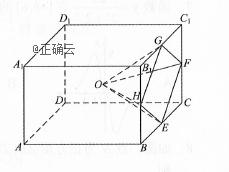
\includegraphics[width=.42\linewidth]{assets/asset-057-01.jpg}
\end{center}
\fillin[{$118.8$}]
\begin{solution}
\textbf{答案：}$118.8$

\textbf{分析：}根据题意可知模型的体积为长方体体积与四棱锥体积之差，进而求得模型的体积，再求出模型的质量。

\textbf{详解：}由题意得，四棱锥 $O-EFGH$ 的底面积为 $4\times 6 - 4\times \dfrac{1}{2}\times 2\times 3 = 12\text{ cm}^2$，其高为点 $O$ 到底面 $BB_1C_1C$ 的距离 $3\text{ cm}$，则此四棱锥的体积为 $V_1 = \dfrac{1}{3}\times 12\times 3 = 12\text{ cm}^3$。又长方体 $ABCD-A_1B_1C_1D_1$ 的体积为 $V_2 = 4\times 6\times 6 = 144\text{ cm}^3$，所以该模型体积 $V = V_2 - V_1 = 132\text{ cm}^3$，其质量为 $0.9\times 132 = 118.8\text{ g}$。
\end{solution}
\end{question}

\begin{question}[points=12]
\textbf{来源：}2019 年 全国III卷-理科，第 19 题\par
图 1 是由矩形 $ADEB$、$\text{Rt}\triangle ABC$ 和菱形 $BFGC$ 组成的一个平面图形，其中 $AB=1$，$BE=BF=2$，$\angle FBC=60^\circ$，将其沿 $AB$，$BC$ 折起使得 $BE$ 与 $BF$ 重合，连结 $DG$，如图 2。

（1）证明：图 2 中的 $A$，$C$，$G$，$D$ 四点共面，且平面 $ABC\perp$ 平面 $BCGE$；

（2）求图 2 中的二面角 $B-CG-A$ 的大小。

\begin{center}
  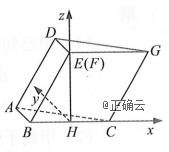
\includegraphics[width=.42\linewidth]{assets/asset-058-01.jpg}
\end{center}
\begin{solution}
\textbf{答案：}（1）见详解；（2）$30^\circ$。

\textbf{分析：}(1)因为折纸和粘合不改变矩形 $ADEB$、$\text{Rt}\triangle ABC$ 和菱形 $BFGC$ 内部的夹角，所以 $AD\parallel BE$，$BF\parallel CG$ 依然成立，又因 $E$ 和 $F$ 粘在一起，所以得证。因为 $AB$ 是平面 $BCGE$ 的垂线，所以易证。(2)在图中找到 $B-CG-A$ 对应的平面角，再求此平面角即可。

\textbf{详解：}（1）由已知得 $AD\parallel BE$，$CG\parallel BE$，所以 $AD\parallel CG$，故 $AD$，$CG$ 确定一个平面，从而 $A$，$C$，$G$，$D$ 四点共面。由已知得 $AB\perp BE$，$AB\perp BC$，故 $AB\perp$ 平面 $BCGE$。又因为 $AB\subset$ 平面 $ABC$，所以平面 $ABC\perp$ 平面 $BCGE$。
（2）作 $EH\perp BC$，垂足为 $H$。因为 $EH\subset$ 平面 $BCGE$，平面 $BCGE\perp$ 平面 $ABC$，所以 $EH\perp$ 平面 $ABC$。由已知，菱形 $BCGE$ 的边长为 $2$，$\angle EBC=60^\circ$，可求得 $BH=1$，$EH=\sqrt{3}$。以 $H$ 为坐标原点，$\overrightarrow{HC}$ 的方向为 $x$ 轴的正方向，建立如图所示的空间直角坐标系 $H-xyz$，则 $A(-1,1,0)$，$C(1,0,0)$，$G(2,0,\sqrt{3})$，$\overrightarrow{CG}=(1,0,\sqrt{3})$，$\overrightarrow{AC}=(2,-1,0)$。设平面 $ACGD$ 的法向量为 $\mathbf{n}=(x,y,z)$，则 $\begin{cases} \overrightarrow{CG}\cdot\mathbf{n}=0 \\ \overrightarrow{AC}\cdot\mathbf{n}=0 \end{cases}$，即 $\begin{cases} x+\sqrt{3}z=0 \\ 2x-y=0 \end{cases}$，可取 $\mathbf{n}=(3,6,-\sqrt{3})$。又平面 $BCGE$ 的法向量可取为 $\mathbf{m}=(0,1,0)$，所以 $\cos\langle\mathbf{n},\mathbf{m}\rangle = \dfrac{\mathbf{n}\cdot\mathbf{m}}{|\mathbf{n}||\mathbf{m}|} = \dfrac{6}{\sqrt{48}} = \dfrac{\sqrt{3}}{2}$。因此二面角 $B-CG-A$ 的大小为 $30^\circ$。
\end{solution}
\end{question}

\begin{question}[points=5]
\textbf{来源：}2019 年 全国III卷-文科，第 8 题\par
如图，点N为正方形ABCD的中心，$\triangle ECD$为正三角形，平面$ECD\perp$平面ABCD，M是线段ED的中点，则
\begin{choices}
  \item $BM=EN$，且直线BM、EN是相交直线
  \item $BM\neq EN$，且直线BM、EN是相交直线
  \item $BM=EN$，且直线BM、EN是异面直线
  \item $BM\neq EN$，且直线BM、EN是异面直线
\end{choices}
\begin{solution}
\textbf{答案：}B

\textbf{分析：}利用垂直关系，再结合勾股定理进而解决问题。

\textbf{详解：}$\because \triangle BDE$，N为BD中点，M为DE中点，$\therefore BM,EN$共面相交，选项C，D为错。作$EO\perp CD$于O，连接ON，过M作$MF\perp OD$于F。连BF，$\because$平面$CDE\perp$平面ABCD。$EO\perp CD,EO\subset$平面CDE，$\therefore EO\perp$平面ABCD，$MF\perp$平面ABCE，$\therefore \triangle MFB$与$\triangle EON$均为直角三角形。设正方形边长为2，易知$EO=\sqrt{3},ON=1$，$EN=2$，$MF=\frac{\sqrt{3}}{2},BF=\sqrt{2^2+(\frac{3}{2})^2}=\frac{5}{2}$，$\therefore BM=\sqrt{\frac{3}{4}+\frac{25}{4}}=\sqrt{7}$。$\therefore BM\neq EN$，故选B。
\end{solution}
\end{question}

\begin{question}[points=5]
\textbf{来源：}2019 年 全国III卷-文科，第 16 题\par
学生到工厂劳动实践，利用3D打印技术制作模型。如图，该模型为长方体$ABCD-A_1B_1C_1D_1$挖去四棱锥$O-EFGH$后所得的几何体，其中O为长方体的中心，E,F,G,H分别为所在棱的中点，$AB=BC=6cm, AA_1=4cm$，3D打印所用原料密度为$0.9g/cm^3$，不考虑打印损耗，制作该模型所需原料的质量为g。

\begin{center}
  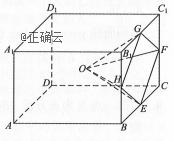
\includegraphics[width=.42\linewidth]{assets/asset-060-01.jpg}
\end{center}
\fillin[{$118.8$}]
\begin{solution}
\textbf{答案：}$118.8$

\textbf{分析：}根据题意可知模型的体积为长方体体积与四棱锥体积之差进而求得模型的体积，再求出模型的质量。

\textbf{详解：}由题意得，四棱锥$O-EFGH$的底面积为$4\times6-4\times\frac{1}{2}\times2\times3=12cm^2$，其高为点O到底面$BB_1C_1C$的距离为$3cm$，则此四棱锥的体积为$V_1=\frac{1}{3}\times12\times3=12cm^3$。又长方体$ABCD-A_1B_1C_1D_1$的体积为$V_2=4\times6\times6=144cm^3$，所以该模型体积为$V=V_2-V_1=144-12=132cm^3$，其质量为$0.9\times132=118.8g$。
\end{solution}
\end{question}

\begin{question}[points=12]
\textbf{来源：}2019 年 全国III卷-文科，第 19 题\par
图1是由矩形ADEB、$Rt\triangle ABC$和菱形BFGC组成的一个平面图形，其中AB=1，BE=BF=2，$\angle FBC=60^\circ$。将其沿AB，BC折起使得BE与BF重合，连结DG，如图2。

(1)证明图2中的A,C,G,D四点共面，且平面$ABC\perp$平面BCGE；

(2)求图2中的四边形ACGD的面积。

\begin{center}
  
\includegraphics[width=.42\linewidth]{assets/asset-061-01.jpg}
\end{center}
\begin{solution}
\textbf{答案：}(1)见详解; (2)4

\textbf{分析：}(1)因为折纸和粘合不改变矩形ADEB、$Rt\triangle ABC$和菱形BFGC内部的夹角，所以$AD\parallel BE$，$BF\parallel CG$依然成立，又因E和F粘在一起，所以得证。因为AB是平面BCGE的垂线，所以易证平面垂直。(2)欲求四边形ACGD的面积，需求出CG所对应的高，然后乘以CG即可。

\textbf{详解：}(1)证：$\because AD\parallel BE$，$BF\parallel CG$，又因为E和F粘在一起。$\therefore AD\parallel CG$，A,C,G,D四点共面。又$\because AB\perp BE$，$AB\perp BC$。$\therefore AB\perp$平面BCGE，$\because AB\subset$平面ABC，$\therefore$平面$ABC\perp$平面BCGE，得证。
(2)取CG的中点M，连结EM,DM。因为$AB\parallel DE$，$AB\perp$平面BCGE，所以$DE\perp$平面BCGE，故$DE\perp CG$。由已知，四边形BCGE是菱形，且$\angle EBC=60^\circ$得$EM\perp CG$，故$CG\perp$平面DEM。因此$DM\perp CG$。在$Rt\triangle DEM$中，DE=1，$EM=\sqrt{3}$，故$DM=2$。所以四边形ACGD的面积为$2\times2=4$。
\end{solution}
\end{question}

\begin{question}[points=5]
\textbf{来源：}2019 年 全国II卷-理科，第 7 题\par
设 $\alpha$，$\beta$ 为两个平面，则 $\alpha\parallel\beta$ 的充要条件是
\begin{choices}
  \item $\alpha$ 内有无数条直线与 $\beta$ 平行
  \item $\alpha$ 内有两条相交直线与 $\beta$ 平行
  \item $\alpha$，$\beta$ 平行于同一条直线
  \item $\alpha$，$\beta$ 垂直于同一平面
\end{choices}
\begin{solution}
\textbf{答案：}$B$

\textbf{分析：}本题考查了空间两个平面的判定与性质及充要条件，渗透直观想象、逻辑推理素养，利用面面平行的判定定理与性质定理即可作出判断．

\textbf{详解：}由面面平行的判定定理知：$\alpha$ 内两条相交直线都与 $\beta$ 平行是 $\alpha\parallel\beta$ 的充分条件，由面面平行性质定理知，若 $\alpha\parallel\beta$，则 $\alpha$ 内任意一条直线都与 $\beta$ 平行，所以 $\alpha$ 内两条相交直线都与 $\beta$ 平行是 $\alpha\parallel\beta$ 的必要条件，故选 $B$．
\end{solution}
\end{question}

\begin{question}[points=5]
\textbf{来源：}2019 年 全国II卷-理科，第 16 题\par
中国有悠久的金石文化，印信是金石文化的代表之一．印信的形状多为长方体、正方体或圆柱体，但南北朝时期的官员独孤信的印信形状是“半正多面体”（图 1）．半正多面体是由两种或两种以上的正多边形围成的多面体．半正多面体体现了数学的对称美．图 2 是一个棱数为 48 的半正多面体，它的所有顶点都在同一个正方体的表面上，且此正方体的棱长为 1．则该半正多面体共有个面，其棱长为．（本题第一空 2 分，第二空 3 分．）
\fillin[{26；$\sqrt{2}-1$}]
\begin{solution}
\textbf{答案：}26；$\sqrt{2}-1$

\textbf{分析：}第一问可按题目数出来，第二问需在正方体中简单还原出物体位置，利用对称性，平面几何解决．

\textbf{详解：}由图可知第一层与第三层各有 9 个面，计 18 个面，第二层共有 8 个面，所以该半正多面体共有 $18+8=26$ 个面．如图，设该半正多面体的棱长为 $x$，则 $AB=BE=x$，延长 $BC$ 与 $FE$ 交于点 $G$，延长 $BC$ 交正方体棱于 $H$，由半正多面体对称性可知，$\triangle BGE$ 为等腰直角三角形，$\therefore BG=GE=CH=\frac{\sqrt{2}}{2}x$，$\therefore GH=2\times\frac{\sqrt{2}}{2}x+x=(\sqrt{2}+1)x=1$，$\therefore x=\frac{1}{\sqrt{2}+1}=\sqrt{2}-1$．
\end{solution}
\end{question}

\begin{question}[points=12]
\textbf{来源：}2019 年 全国II卷-理科，第 17 题\par
如图，长方体 $ABCD-A_1B_1C_1D_1$ 的底面 $ABCD$ 是正方形，点 $E$ 在棱 $AA_1$ 上，$BE\perp EC_1$．

（1）证明：$BE\perp$ 平面 $EB_1C_1$；

（2）若 $AE=A_1E$，求二面角 $B-EC-C_1$ 的正弦值．
\begin{solution}
\textbf{答案：}$\frac{\sqrt{3}}{2}$

\textbf{分析：}（1）利用长方体的性质，可以知道 $B_1C_1\perp$ 侧面 $A_1B_1BA$，利用线面垂直的性质可以证明出 $B_1C_1\perp EB$，这样可以利用线面垂直的判定定理，证明出 $BE\perp$ 平面 $EB_1C_1$；（2）建立空间直角坐标系，求出相关向量，利用法向量求二面角．

\textbf{详解：}（1）由已知得，$B_1C_1\perp$ 平面 $ABB_1A_1$，$BE\subset$ 平面 $ABB_1A_1$，故 $B_1C_1\perp BE$．又 $BE\perp EC_1$，所以 $BE\perp$ 平面 $EB_1C_1$．
（2）由（1）知 $\angle BEB_1=90^\circ$．由题设知 $\triangle ABE\cong\triangle A_1B_1E$，所以 $\angle AEB=45^\circ$，故 $AE=AB$，$AA_1=2AB$．以 $D$ 为坐标原点，$\overrightarrow{DA}$ 的方向为 $x$ 轴正方向，$|\overrightarrow{DA}|$ 为单位长，建立如图所示的空间直角坐标系 $D-xyz$，则 $C(0,1,0)$，$B(1,1,0)$，$C_1(0,1,2)$，$E(1,0,1)$，$\overrightarrow{CE}=(1,-1,1)$，$\overrightarrow{CC_1}=(0,0,2)$．设平面 $EBC$ 的法向量为 $\mathbf{n}=(x,y,z)$，由 $\begin{cases} \mathbf{n}\cdot\overrightarrow{CB}=0 \\ \mathbf{n}\cdot\overrightarrow{CE}=0 \end{cases}$ 得 $\begin{cases} x=0 \\ x-y+z=0 \end{cases}$，可取 $\mathbf{n}=(0,-1,-1)$．设平面 $ECC_1$ 的法向量为 $\mathbf{m}=(x,y,z)$，由 $\begin{cases} \mathbf{m}\cdot\overrightarrow{CC_1}=0 \\ \mathbf{m}\cdot\overrightarrow{CE}=0 \end{cases}$ 得 $\begin{cases} 2z=0 \\ x-y+z=0 \end{cases}$，可取 $\mathbf{m}=(1,1,0)$．于是 $\cos\langle\mathbf{n},\mathbf{m}\rangle=\frac{\mathbf{n}\cdot\mathbf{m}}{|\mathbf{n}||\mathbf{m}|}=-\frac{1}{2}$．所以二面角 $B-EC-C_1$ 的正弦值为 $\sqrt{1-(-\frac{1}{2})^2}=\frac{\sqrt{3}}{2}$．
\end{solution}
\end{question}

\begin{question}[points=5]
\textbf{来源：}2019 年 全国II卷-文科，第 7 题\par
设 $\alpha,\beta$ 为两个平面，则 $\alpha\parallel\beta$ 的充要条件是
\begin{choices}
  \item $\alpha$ 内有无数条直线与 $\beta$ 平行
  \item $\alpha$ 内有两条相交直线与 $\beta$ 平行
  \item $\alpha,\beta$ 平行于同一条直线
  \item $\alpha,\beta$ 垂直于同一平面
\end{choices}
\begin{solution}
\textbf{答案：}$B$

\textbf{分析：}本题考查了空间两个平面的判定与性质及充要条件，渗透直观想象、逻辑推理素养，利用面面平行的判定定理与性质定理即可作出判断．

\textbf{详解：}由面面平行的判定定理知：$\alpha$ 内两条相交直线都与 $\beta$ 平行是 $\alpha/\!\/\beta$ 的充分条件，由面面平行性质定理知，若 $\alpha/\!\/\beta$，则 $\alpha$ 内任意一条直线都与 $\beta$ 平行，所以 $\alpha$ 内两条相交直线都与 $\beta$ 平行是 $\alpha/\!\/\beta$ 的必要条件，故选 $B$．
\end{solution}
\end{question}

\begin{question}[points=5]
\textbf{来源：}2019 年 全国II卷-文科，第 16 题\par
中国有悠久的金石文化，印信是金石文化的代表之一．印信的形状多为长方体、正方体或圆柱体，但南北朝时期的官员独孤信的印信形状是“半正多面体”（图 $1$）．半正多面体是由两种或两种以上的正多边形围成的多面体．半正多面体体现了数学的对称美．图 $2$ 是一个棱数为 $48$ 的半正多面体，它的所有顶点都在同一个正方体的表面上，且此正方体的棱长为 $1$．则该半正多面体共有个面，其棱长为．（本题第一空 $2$ 分，第二空 $3$ 分．）
\fillin[{$26$ 个面，$\sqrt{2}-1$}]
\begin{solution}
\textbf{答案：}$26$ 个面，$\sqrt{2}-1$

\textbf{分析：}第一问可按题目数出来，第二问需在正方体中简单还原出物体位置，利用对称性，平面几何解决．

\textbf{详解：}由图可知第一层与第三层各有 $9$ 个面，计 $18$ 个面，第二层共有 $8$ 个面，所以该半正多面体共有 $18+8=26$ 个面．如图，设该半正多面体的棱长为 $x$，则 $AB=BE=x$，延长 $BC$ 与 $FE$ 交于点 $G$，延长 $BC$ 交正方体棱于 $H$，由半正多面体对称性可知，$\triangle BGE$ 为等腰直角三角形，$\therefore BG=GE=CH=\dfrac{\sqrt{2}}{2}x$，$\therefore GH=2\times\dfrac{\sqrt{2}}{2}x+x=(\sqrt{2}+1)x=1$，$\therefore x=\dfrac{1}{\sqrt{2}+1}=\sqrt{2}-1$，即该半正多面体棱长为 $\sqrt{2}-1$．
\end{solution}
\end{question}

\begin{question}[points=12]
\textbf{来源：}2019 年 全国II卷-文科，第 17 题\par
如图，长方体 $ABCD-A_1B_1C_1D_1$ 的底面 $ABCD$ 是正方形，点 $E$ 在棱 $AA_1$ 上，$BE\perp EC_1$．

（1）证明：$BE\perp$ 平面 $EB_1C_1$；

（2）若 $AE=A_1E$，$AB=3$，求四棱锥 $E-BB_1C_1C$ 的体积．

\begin{center}
  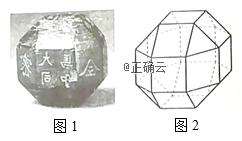
\includegraphics[width=.42\linewidth]{assets/asset-067-01.jpg}
\end{center}
\begin{solution}
\textbf{答案：}（1）见详解；（2）$18$

\textbf{分析：}（1）先由长方体得，$B_1C_1\perp$ 平面 $AA_1B_1B$，得到 $B_1C_1\perp BE$，再由 $BE\perp EC_1$，根据线面垂直的判定定理，即可证明结论成立；
（2）先设长方体侧棱长为 $2a$，根据题中条件求出 $a=3$；再取 $BB_1$ 中点 $F$，连结 $EF$，证明 $EF\perp$ 平面 $BB_1C_1C$，根据四棱锥的体积公式，即可求出结果．

\textbf{详解：}（1）因为在长方体 $ABCD-A_1B_1C_1D_1$ 中，$B_1C_1\perp$ 平面 $AA_1B_1B$；$BE\subset$ 平面 $AA_1B_1B$，所以 $B_1C_1\perp BE$，又 $BE\perp EC_1$，$B_1C_1\cap EC_1=C_1$，且 $EC_1\subset$ 平面 $EB_1C_1$，$B_1C_1\subset$ 平面 $EB_1C_1$，所以 $BE\perp$ 平面 $EB_1C_1$．
（2）设长方体侧棱长为 $2a$，则 $AE=A_1E=a$，由（1）可得 $EB_1\perp BE$；所以 $EB_1^2+BE^2=BB_1^2$，即 $2BE^2=BB_1^2$，又 $AB=3$，所以 $2AE^2+2AB^2=BB_1^2$，即 $2a^2+18=4a^2$，解得 $a=3$；取 $BB_1$ 中点 $F$，连结 $EF$，因为 $AE=A_1E$，则 $EF\parallel AB$；所以 $EF\perp$ 平面 $BB_1C_1C$，所以四棱锥 $E-BB_1C_1C$ 的体积为 $V_{E-BB_1C_1C}=\dfrac{1}{3}S_{\text{矩形}BB_1C_1C}\cdot EF=\dfrac{1}{3}\cdot BC\cdot BB_1\cdot EF=\dfrac{1}{3}\times3\times6\times3=18$．
\end{solution}
\end{question}

\begin{question}[points=5]
\textbf{来源：}2019 年 全国I卷-理科，第 12 题\par
已知三棱锥 $P-ABC$ 的四个顶点在球 $O$ 的球面上，$PA = PB = PC$，$\triangle ABC$ 是边长为 $2$ 的正三角形，$E$, $F$ 分别是 $PA$, $PB$ 的中点，$\angle CEF = 90^\circ$，则球 $O$ 的体积为
\begin{choices}
  \item $8\sqrt{6}\pi$
  \item $4\sqrt{6}\pi$
  \item $2\sqrt{6}\pi$
  \item $\sqrt{6}\pi$
\end{choices}
\begin{solution}
\textbf{答案：}$D$

\textbf{分析：}本题也可用解三角形方法，达到求出棱长的目的．适合空间想象能力略差学生．设 $PA = PB = PC = 2x$, $E$, $F$ 分别为 $PA$, $AB$ 中点，$\therefore EF \parallel PB$，且 $EF = \frac{1}{2}PB = x$，$\because \triangle ABC$ 为边长为 $2$ 的等边三角形，$\therefore CF = \sqrt{3}$ 又 $\angle CEF = 90^\circ$ $\therefore CE = \sqrt{3 - x^2}$, $AE = \frac{1}{2}PA = x$ $\triangle AEC$ 中余弦定理 $\cos \angle EAC = \frac{x^2 + 4 - (3 - x^2)}{2 \times 2 \times x}$，作 $PD \perp AC$ 于 $D$，$\because PA = PC$，$\therefore D$ 为 $AC$ 中点，$\cos \angle EAC = \frac{AD}{PA} = \frac{1}{2x}$，$\therefore \frac{x^2 + 4 - 3 + x^2}{4x} = \frac{1}{2x}$，$\therefore 2x^2 + 1 = 2$ $\therefore x^2 = \frac{1}{2}$ $x = \frac{\sqrt{2}}{2}$，$\therefore PA = PB = PC = \sqrt{2}$，又 $AB = BC = AC = 2$，$\therefore PA$, $PB$, $PC$ 两两垂直，$\therefore 2R = \sqrt{2 + 2 + 2} = \sqrt{6}$，$\therefore R = \frac{\sqrt{6}}{2}$，$\therefore V = \frac{4}{3}\pi R^3 = \frac{4}{3}\pi \times \frac{6\sqrt{6}}{8} = \sqrt{6}\pi$，故选 $D$．

\textbf{详解：}$\because PA = PB = PC$, $\triangle ABC$ 为边长为 $2$ 的等边三角形，$\therefore P-ABC$ 为正三棱锥，$\therefore PB \perp AC$，又 $E$, $F$ 分别为 $PA$, $AB$ 中点，$\therefore EF \parallel PB$，$\therefore EF \perp AC$，又 $EF \perp CE$, $CE \cap AC = C$, $\therefore EF \perp$ 平面 $PAC$，$PB \perp$ 平面 $PAC$，$\therefore \angle PAB = 90^\circ$, $\therefore PA = PB = PC = \sqrt{2}$，$\therefore P-ABC$ 为正方体一部分，$2R = \sqrt{2 + 2 + 2} = \sqrt{6}$，即 $R = \frac{\sqrt{6}}{2}$, $\therefore V = \frac{4}{3}\pi R^3 = \frac{4}{3}\pi \times \frac{6\sqrt{6}}{8} = \sqrt{6}\pi$，故选 $D$．
\end{solution}
\end{question}

\begin{question}[points=12]
\textbf{来源：}2019 年 全国I卷-理科，第 18 题\par
如图，直四棱柱 $ABCD-A_1B_1C_1D_1$ 的底面是菱形，$AA_1 = 4$, $AB = 2$, $\angle BAD = 60^\circ$, $E$, $M$, $N$ 分别是 $BC$, $BB_1$, $A_1D$ 的中点．

(1) 证明：$MN \parallel$ 平面 $C_1DE$;

(2) 求二面角 $A-MA_1-N$ 的正弦值．

\begin{center}
  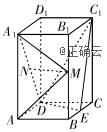
\includegraphics[width=.42\linewidth]{assets/asset-069-01.jpg}
\end{center}
\begin{solution}
\textbf{答案：}(1) 见解析; (2) $\frac{\sqrt{10}}{5}$

\textbf{分析：}(1) 利用三角形中位线和 $A_1D \parallel B_1C$ 可证得 $ME \parallel ND$，证得四边形 $MNDE$ 为平行四边形，进而证得 $MN \parallel DE$，根据线面平行判定定理可证得结论；(2) 以菱形 $ABCD$ 对角线交点为原点可建立空间直角坐标系，通过取 $AB$ 中点 $F$，可证得 $DF \perp$ 平面 $AMA_1$，得到平面 $AMA_1$ 的法向量 $\overrightarrow{DF}$；再通过向量法求得平面 $MA_1N$ 的法向量 $\mathbf{n}$，利用向量夹角公式求得两个法向量夹角的余弦值，进而可求得所求二面角的正弦值．

\textbf{详解：}(1) 连接 $ME$, $B_1C$．$\because M$, $E$ 分别为 $BB_1$, $BC$ 中点，$\therefore ME$ 为 $\triangle B_1BC$ 的中位线，$\therefore ME \parallel B_1C$ 且 $ME = \frac{1}{2}B_1C$．又 $N$ 为 $A_1D$ 中点，且 $A_1D \parallel B_1C$，$\therefore ND \parallel B_1C$ 且 $ND = \frac{1}{2}B_1C$，$\therefore ME \parallel ND$，$\therefore$ 四边形 $MNDE$ 为平行四边形，$\therefore MN \parallel DE$，又 $MN \not\subset$ 平面 $C_1DE$, $DE \subset$ 平面 $C_1DE$，$\therefore MN \parallel$ 平面 $C_1DE$．
(2) 设 $AC \cap BD = O$, $A_1C_1 \cap B_1D_1 = O_1$，由直四棱柱性质可知：$OO_1 \perp$ 平面 $ABCD$．$\because$ 四边形 $ABCD$ 为菱形，$\therefore AC \perp BD$．则以 $O$ 为原点，可建立如图所示的空间直角坐标系．则 $A(\sqrt{3}, 0, 0)$, $M(0, 1, 2)$, $A_1(\sqrt{3}, 0, 4)$, $D(0, -1, 0)$, $N\left(\frac{\sqrt{3}}{2}, -\frac{1}{2}, 2\right)$．取 $AB$ 中点 $F$，连接 $DF$，则 $F\left(\frac{\sqrt{3}}{2}, \frac{1}{2}, 0\right)$．$\because$ 四边形 $ABCD$ 为菱形且 $\angle BAD = 60^\circ$，$\therefore \triangle BAD$ 为等边三角形，$\therefore DF \perp AB$．又 $AA_1 \perp$ 平面 $ABCD$, $DF \subset$ 平面 $ABCD$，$\therefore DF \perp AA_1$，$\therefore DF \perp$ 平面 $ABB_1A_1$，即 $DF \perp$ 平面 $AMA_1$，$\therefore \overrightarrow{DF}$ 为平面 $AMA_1$ 的一个法向量，且 $\overrightarrow{DF} = \left(\frac{\sqrt{3}}{2}, \frac{3}{2}, 0\right)$．设平面 $MA_1N$ 的法向量 $\mathbf{n} = (x, y, z)$，又 $\overrightarrow{MA_1} = (\sqrt{3}, -1, 2)$, $\overrightarrow{MN} = \left(\frac{\sqrt{3}}{2}, -\frac{3}{2}, 0\right)$，$\because \begin{cases} \mathbf{n} \cdot \overrightarrow{MA_1} = \sqrt{3}x - y + 2z = 0 \\ \mathbf{n} \cdot \overrightarrow{MN} = \frac{\sqrt{3}}{2}x - \frac{3}{2}y = 0 \end{cases}$，令 $x = \sqrt{3}$，则 $y = 1$, $z = -1$，$\therefore \mathbf{n} = (\sqrt{3}, 1, -1)$．$\therefore \cos \langle \overrightarrow{DF}, \mathbf{n} \rangle = \frac{\overrightarrow{DF} \cdot \mathbf{n}}{|\overrightarrow{DF}| |\mathbf{n}|} = \frac{3}{\sqrt{15} \times \sqrt{5}} = \frac{\sqrt{3}}{5}$，$\therefore \sin \langle \overrightarrow{DF}, \mathbf{n} \rangle = \frac{\sqrt{10}}{5}$．$\therefore$ 二面角 $A-MA_1-N$ 的正弦值为 $\frac{\sqrt{10}}{5}$．
\end{solution}
\end{question}

\begin{question}[points=5]
\textbf{来源：}2019 年 全国I卷-文科，第 16 题\par
已知 $\angle ACB = 90°$，$P$ 为平面 $ABC$ 外一点，$PC=2$，点 $P$ 到 $\angle ACB$ 两边 $AC$，$BC$ 的距离均为 $\sqrt{3}$，那么 $P$ 到平面 $ABC$ 的距离为．
\fillin[{$\sqrt{2}$}]
\begin{solution}
\textbf{答案：}$\sqrt{2}$

\textbf{分析：}本题考查学生空间想象能力，合理画图成为关键，准确找到 $P$ 在底面上的射影，使用线面垂直定理，得到垂直关系，勾股定理解决。

\textbf{详解：}作 $PD$，$PE$ 分别垂直于 $AC$，$BC$，$PO \perp$ 平面 $ABC$，连 $CO$，知 $CD \perp PD$，$CD \perp PO$，$PD \cap OD = P$，所以 $CD \perp$ 平面 $PDO$，$OD \subset$ 平面 $PDO$，$\Rightarrow CD \perp OD$。因为 $PD = PE = \sqrt{3}$，$PC=2$，所以 $\sin\angle PCE = \sin\angle PCD = \frac{\sqrt{3}}{2}$，$\Rightarrow \angle PCB = \angle PCA = 60°$，$\Rightarrow PO \perp CO$，$CO$ 为 $\angle ACB$ 平分线，$\Rightarrow \angle OCD = 45°$，$\Rightarrow OD = CD = 1$，$OC = \sqrt{2}$，又 $PC=2$，$\Rightarrow PO = \sqrt{4-2} = \sqrt{2}$。
\end{solution}
\end{question}

\begin{question}[points=12]
\textbf{来源：}2019 年 全国I卷-文科，第 19 题\par
如图，直四棱柱 $ABCD-A_1B_1C_1D_1$ 的底面是菱形，$AA_1=4$，$AB=2$，$\angle BAD=60°$，$E$，$M$，$N$ 分别是 $BC$，$BB_1$，$A_1D$ 的中点．

（1）证明：$MN \parallel$ 平面 $C_1DE$；

（2）求点 $C$ 到平面 $C_1DE$ 的距离．

\begin{center}
  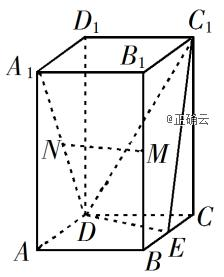
\includegraphics[width=.42\linewidth]{assets/asset-071-01.jpg}
\end{center}
\begin{solution}
\textbf{答案：}（1）见解析；（2）$\frac{4\sqrt{17}}{17}$。

\textbf{分析：}（1）利用三角形中位线和 $A_1D_1 \parallel BC$ 可证得 $ME \parallel ND$，证得四边形 $MNDE$ 为平行四边形，进而证得 $MN \parallel DE$，根据线面平行判定定理可证得结论；（2）根据题意求得三棱锥 $C_1-CDE$ 的体积，再求出 $\triangle C_1DE$ 的面积，利用等体积法求得点 $C$ 到平面 $C_1DE$ 的距离。

\textbf{详解：}（1）连接 $ME$，$B_1C$．因为 $M$，$E$ 分别为 $BB_1$，$BC$ 中点，所以 $ME$ 为 $\triangle B_1BC$ 的中位线，$\Rightarrow ME \parallel B_1C$ 且 $ME = \frac{1}{2}B_1C$．又 $N$ 为 $A_1D$ 中点，且 $A_1D_1 \parallel BC$，$\Rightarrow ND \parallel B_1C$ 且 $ND = \frac{1}{2}B_1C$，$\Rightarrow ME \parallel ND$，$\Rightarrow$ 四边形 $MNDE$ 为平行四边形，$\Rightarrow MN \parallel DE$，又 $MN \not\subset$ 平面 $C_1DE$，$DE \subset$ 平面 $C_1DE$，$\Rightarrow MN \parallel$ 平面 $C_1DE$。
（2）在菱形 $ABCD$ 中，$E$ 为 $BC$ 中点，所以 $DE \perp BC$，根据题意有 $DE = \sqrt{3}$，$C_1E = \sqrt{17}$，因为棱柱为直棱柱，所以有 $DE \perp$ 平面 $BCC_1B_1$，所以 $DE \perp EC_1$，所以 $S_{\triangle DEC_1} = \frac{1}{2} \times \sqrt{3} \times \sqrt{17}$，设点 $C$ 到平面 $C_1DE$ 的距离为 $d$，根据题意有 $V_{C_1-CDE} = V_{C-C_1DE}$，则有 $\frac{1}{3} \times \frac{1}{2} \times \sqrt{3} \times \sqrt{17} \times d = \frac{1}{3} \times \frac{1}{2} \times 1 \times \sqrt{3} \times 4$，解得 $d = \frac{4}{\sqrt{17}} = \frac{4\sqrt{17}}{17}$，所以点 $C$ 到平面 $C_1DE$ 的距离为 $\frac{4\sqrt{17}}{17}$。
\end{solution}
\end{question}

\section*{2020 年}

\begin{question}[points=5]
\textbf{来源：}2020 年 全国III卷-理科，第 8 题\par
下图为某几何体的三视图，则该几何体的表面积是

\begin{center}
  
\includegraphics[width=.42\linewidth]{assets/asset-072-01.jpg}
\end{center}
\begin{choices}
  \item $6+4\sqrt{2}$
  \item $4+4\sqrt{2}$
  \item $6+2\sqrt{3}$
  \item $4+2\sqrt{3}$
\end{choices}
\begin{solution}
\textbf{答案：}$C$

\textbf{分析：}根据三视图特征，在正方体中截取出符合题意的立体图形，求出每个面的面积。

\textbf{详解：}根据三视图特征，在正方体中截取出如图立体图形。$S_{\triangle ABC}=S_{\triangle ADC}=S_{\triangle CDB}=\dfrac12\times2\times2=2$，$AB=AD=DB=2\sqrt{2}$，$\triangle ADB$ 是边长为 $2\sqrt{2}$ 的等边三角形，$S_{\triangle ADB}=\dfrac12\times(2\sqrt{2})^2\times\sin60^\circ=\dfrac12\times8\times\dfrac{\sqrt{3}}{2}=2\sqrt{3}$。所以表面积 $=3\times2+2\sqrt{3}=6+2\sqrt{3}$。故选 $C$。
\end{solution}
\end{question}

\begin{question}[points=5]
\textbf{来源：}2020 年 全国III卷-理科，第 15 题\par
已知圆锥的底面半径为 $1$，母线长为 $3$，则该圆锥内半径最大的球的体积为 。

\begin{center}
  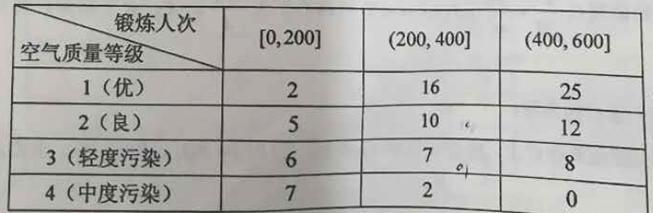
\includegraphics[width=.42\linewidth]{assets/asset-073-01.jpg}
\end{center}
\fillin[{$\dfrac{2}{3}\pi$}]
\begin{solution}
\textbf{答案：}$\dfrac{2}{3}\pi$

\textbf{分析：}半径最大的球为圆锥的内切球，利用轴截面求内切球半径。

\textbf{详解：}圆锥轴截面如图，$BC=2$，$AB=AC=3$，$AM=\sqrt{3^2-1^2}=2\sqrt{2}$。$S_{\triangle ABC}=\frac12\times2\times2\sqrt{2}=2\sqrt{2}$。设内切球半径为 $r$，则 $S_{\triangle ABC}=\frac12(AB+AC+BC)r=\frac12(3+3+2)r=4r$，所以 $4r=2\sqrt{2}$，$r=\frac{\sqrt{2}}{2}$。体积 $V=\frac43\pi r^3=\frac43\pi\left(\frac{\sqrt{2}}{2}\right)^3=\frac{2}{3}\pi$。
\end{solution}
\end{question}

\begin{question}[points=12]
\textbf{来源：}2020 年 全国III卷-理科，第 19 题\par
如图，在长方体 $ABCD-A_1B_1C_1D_1$ 中，点 $E,F$ 分别在棱 $DD_1,BB_1$ 上，且 $2DE=ED_1$，$BF=2FB_1$。

(1) 证明：点 $C_1$ 在平面 $AEF$ 内；

(2) 若 $AB=2$，$AD=1$，$AA_1=3$，求二面角 $A-EF-A_1$ 的正弦值。

\begin{center}
  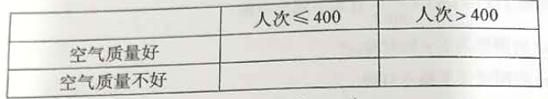
\includegraphics[width=.42\linewidth]{assets/asset-074-01.jpg}
\end{center}
\begin{solution}
\textbf{答案：}见解析

\textbf{分析：}(1) 利用平行四边形的判定证明 $A,E,C_1,F$ 共面；(2) 建立空间直角坐标系，利用向量法求二面角。

\textbf{详解：}(1) 在 $CC_1$ 上取点 $G$ 使得 $C_1G=\frac12CG$，连接 $DG,FG,C_1E,C_1F$。易证 $AF\parallel DG$ 且 $AF=DG$，$C_1E\parallel DG$ 且 $C_1E=DG$，所以 $C_1E\parallel AF$ 且 $C_1E=AF$，四边形 $AEC_1F$ 是平行四边形，所以 $C_1$ 在平面 $AEF$ 内。
(2) 以 $C_1$ 为原点，$C_1D_1,C_1B_1,C_1C$ 为 $x,y,z$ 轴建立空间直角坐标系。$A(2,1,3)$，$A_1(2,1,0)$，$E(2,0,2)$，$F(0,1,1)$。$\overrightarrow{AE}=(0,-1,-1)$，$\overrightarrow{AF}=(-2,0,-2)$，$\overrightarrow{A_1E}=(0,-1,2)$，$\overrightarrow{A_1F}=(-2,0,1)$。设平面 $AEF$ 法向量 $\mathbf{m}=(x_1,y_1,z_1)$，由 $\begin{cases} -y_1-z_1=0 \\ -2x_1-2z_1=0 \end{cases}$ 取 $z_1=-1$，得 $\mathbf{m}=(1,1,-1)$。设平面 $A_1EF$ 法向量 $\mathbf{n}=(x_2,y_2,z_2)$，由 $\begin{cases} -y_2+2z_2=0 \\ -2x_2+z_2=0 \end{cases}$ 取 $z_2=2$，得 $\mathbf{n}=(1,4,2)$。$\cos\langle\mathbf{m},\mathbf{n}\rangle=\dfrac{1+4-2}{\sqrt{3}\times\sqrt{21}}=\dfrac{3}{\sqrt{63}}=\dfrac{\sqrt{7}}{7}$，所以 $\sin\theta=\sqrt{1-\frac{1}{7}}=\dfrac{\sqrt{42}}{7}$。
\end{solution}
\end{question}

\begin{question}[points=5]
\textbf{来源：}2020 年 全国III卷-文科，第 9 题\par
下图为某几何体的三视图，则该几何体的表面积是
\begin{choices}
  \item $6+4\sqrt{2}$
  \item $4+4\sqrt{2}$
  \item $6+2\sqrt{3}$
  \item $4+2\sqrt{3}$
\end{choices}
\begin{solution}
\textbf{答案：}C

\textbf{分析：}根据三视图特征，在正方体中截取出符合题意的立体图形，求出每个面的面积，即可求得其表面积.

\textbf{详解：}根据三视图特征，在正方体中截取出符合题意的立体图形. 根据立体图形可得 $S_{\triangle ABC}=S_{\triangle ADC}=S_{\triangle CDB}=\frac{1}{2}\times2\times2=2$，根据勾股定理可得 $AB=AD=DB=2\sqrt{2}$，所以 $\triangle ADB$ 是边长为 $2\sqrt{2}$ 的等边三角形，其面积为 $\frac{1}{2}\times(2\sqrt{2})^2\times\frac{\sqrt{3}}{2}=2\sqrt{3}$. 故该几何体的表面积为 $3\times2+2\sqrt{3}=6+2\sqrt{3}$. 故选：C.
\end{solution}
\end{question}

\begin{question}[points=5]
\textbf{来源：}2020 年 全国III卷-文科，第 16 题\par
已知圆锥的底面半径为 $1$，母线长为 $3$，则该圆锥内半径最大的球的体积为
\fillin[{$\frac{\sqrt{2}}{3}\pi$}]
\begin{solution}
\textbf{答案：}$\frac{\sqrt{2}}{3}\pi$

\textbf{分析：}将原问题转化为求解圆锥内切球的问题，然后结合截面确定其半径即可确定体积的值.

\textbf{详解：}易知半径最大球为圆锥的内切球，球与圆锥内切时的轴截面如图所示，其中 $BC=2,AB=AC=3$，且点 $M$ 为 $BC$ 边上的中点，设内切圆的圆心为 $O$. 由于 $AM=\sqrt{3^2-1^2}=2\sqrt{2}$，故 $S_{\triangle ABC}=\frac{1}{2}\times2\times2\sqrt{2}=2\sqrt{2}$. 设内切圆半径为 $r$，则 $S_{\triangle ABC}=S_{\triangle AOB}+S_{\triangle BOC}+S_{\triangle AOC}=\frac{1}{2}\times AB\times r+\frac{1}{2}\times BC\times r+\frac{1}{2}\times AC\times r=\frac{1}{2}\times(3+3+2)\times r=2\sqrt{2}$，解得 $r=\frac{\sqrt{2}}{2}$，其体积 $V=\frac{4}{3}\pi r^3=\frac{\sqrt{2}}{3}\pi$.
\end{solution}
\end{question}

\begin{question}[points=12]
\textbf{来源：}2020 年 全国III卷-文科，第 19 题\par
如图，在长方体 $ABCD-A_1B_1C_1D_1$ 中，点 $E$，$F$ 分别在棱 $DD_1$，$BB_1$ 上，且 $2DE=ED_1$，$BF=2FB_1$．证明：

(1) 当 $AB=BC$ 时，$EF\perp AC$；

(2) 点 $C_1$ 在平面 $AEF$ 内．

\begin{center}
  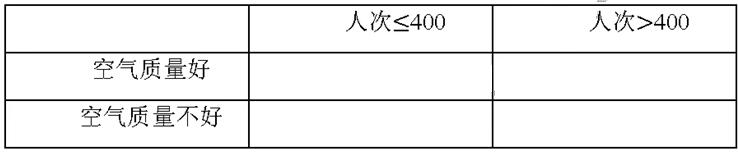
\includegraphics[width=.42\linewidth]{assets/asset-077-01.jpg}
\end{center}
\begin{solution}
\textbf{答案：}证明见解析

\textbf{分析：}(1)根据正方形性质得 $AC\perp BD$，根据长方体性质得 $AC\perp BB_1$，进而可证 $AC\perp$ 平面 $BB_1D_1D$，即得结果；(2)只需证明 $EC_1\parallel AF$ 即可，在 $CC_1$ 上取点 $M$ 使得 $CM=2MC_1$，再通过平行四边形性质进行证明即可.

\textbf{详解：}(1) 因为长方体 $ABCD-A_1B_1C_1D_1$，所以 $BB_1\perp$ 平面 $ABCD$，所以 $AC\perp BB_1$. 因为 $AB=BC$，所以四边形 $ABCD$ 为正方形，所以 $AC\perp BD$. 因为 $BB_1\cap BD=B$，$BB_1,BD\subset$ 平面 $BB_1D_1D$，因此 $AC\perp$ 平面 $BB_1D_1D$. 因为 $EF\subset$ 平面 $BB_1D_1D$，所以 $AC\perp EF$.
(2) 在 $CC_1$ 上取点 $M$ 使得 $CM=2MC_1$，连接 $DM,MF$. 因为 $D_1E=2ED$，$DD_1\parallel CC_1$，$DD_1=CC_1$，所以 $ED=MC_1$，$ED\parallel MC_1$，所以四边形 $DMC_1E$ 为平行四边形，所以 $DM\parallel EC_1$. 因为 $MF\parallel DA$，$MF=DA$，所以四边形 $MFAD$ 为平行四边形，所以 $DM\parallel AF$，所以 $EC_1\parallel AF$，因此 $C_1$ 在平面 $AEF$ 内.
\end{solution}
\end{question}

\begin{question}[points=5]
\textbf{来源：}2020 年 全国II卷-理科，第 7 题\par
如图是一个多面体的三视图，这个多面体某条棱的一个端点在正视图中对应的点为$M$，在俯视图中对应的点为$N$，则该端点在侧视图中对应的点为（ ）

\begin{center}
  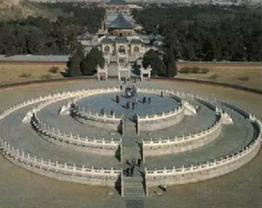
\includegraphics[width=.42\linewidth]{assets/asset-078-01.jpg}
\end{center}
\begin{choices}
  \item E
  \item F
  \item G
  \item H
\end{choices}
\begin{solution}
\textbf{答案：}E

\textbf{分析：}根据三视图，画出多面体立体图形，即可求得M点在侧视图中对应的点.

\textbf{详解：}根据三视图，画出多面体立体图形，图中标出了根据三视图M点所在位置，可知在侧视图中所对应的点为E.
\end{solution}
\end{question}

\begin{question}[points=5]
\textbf{来源：}2020 年 全国II卷-理科，第 10 题\par
已知$\triangle ABC$是面积为$\dfrac{9\sqrt3}{4}$的等边三角形，且其顶点都在球$O$的球面上.若球$O$的表面积为$16\pi$，则$O$到平面$ABC$的距离为（ ）
\begin{choices}
  \item $\sqrt3$
  \item $\dfrac{3}{2}$
  \item 1
  \item $\dfrac{\sqrt3}{2}$
\end{choices}
\begin{solution}
\textbf{答案：}1

\textbf{分析：}根据球O的表面积和$\triangle ABC$的面积可求得球O的半径R和$\triangle ABC$外接圆半径r，由球的性质可知所求距离$d=\sqrt{R^2-r^2}$.

\textbf{详解：}设球O的半径为R，则$4\pi R^2=16\pi$，解得$R=2$.设$\triangle ABC$外接圆半径为r，边长为a，$\triangle ABC$是面积为$\dfrac{9\sqrt3}{4}$的等边三角形，$\therefore\dfrac12 a^2\times\dfrac{\sqrt3}{2}=\dfrac{9\sqrt3}{4}$，解得$a=3$，$\therefore r=\dfrac23\times\sqrt{a^2-\frac{a^2}{4}}=\dfrac23\times\sqrt{9-\frac94}=\dfrac23\times\frac{3\sqrt3}{2}=\sqrt3$，$\therefore$球心O到平面ABC的距离$d=\sqrt{R^2-r^2}=\sqrt{4-3}=1$.
\end{solution}
\end{question}

\begin{question}[points=12]
\textbf{来源：}2020 年 全国II卷-理科，第 20 题\par
如图，已知三棱柱$ABC-A_1B_1C_1$的底面是正三角形，侧面$BB_1C_1C$是矩形，$M,N$分别为$BC,B_1C_1$的中点，$P$为$AM$上一点，过$B_1C_1$和$P$的平面交$AB$于$E$，交$AC$于$F$.

（1）证明：$AA_1\parallel MN$，且平面$A_1AMN\perp$平面$EB_1C_1F$；

（2）设$O$为$\triangle A_1B_1C_1$的中心，若$AO\parallel$平面$EB_1C_1F$，且$AO=AB$，求直线$B_1E$与平面$A_1AMN$所成角的正弦值.
\begin{solution}
\textbf{答案：}（1）证明见解析；（2）$\dfrac{\sqrt{10}}{10}$

\textbf{分析：}（1）由$M,N$分别为$BC,B_1C_1$的中点，$MN\parallel CC_1$，根据条件可得$AA_1\parallel BB_1$，可证$MN\parallel AA_1$，要证平面$EB_1C_1F\perp$平面$A_1AMN$，只需证明$EF\perp$平面$A_1AMN$即可；（2）连接$NP$，先求证四边形$ONPA$是平行四边形，根据几何关系求得$EP$，在$B_1C_1$截取$B_1Q=EP$，由（1）$BC\perp$平面$A_1AMN$，可得$\angle QPN$为$B_1E$与平面$A_1AMN$所成角，即可求得答案.

\textbf{详解：}（1）$\because M,N$分别为$BC,B_1C_1$的中点，$\therefore MN\parallel BB_1$，又$AA_1\parallel BB_1$，$\therefore MN\parallel AA_1$，在$\triangle ABC$中，$M$为$BC$中点，则$BC\perp AM$，又$\because$侧面$BB_1C_1C$为矩形，$\therefore BC\perp BB_1$，$\because MN\parallel BB_1$，$\therefore MN\perp BC$，由$MN\cap AM=M$，$MN,AM\subset$平面$A_1AMN$，$\therefore BC\perp$平面$A_1AMN$，又$\because B_1C_1\parallel BC$，且$B_1C_1\not\subset$平面$ABC$，$BC\subset$平面$ABC$，$\therefore B_1C_1\parallel$平面$ABC$，又$\because B_1C_1\subset$平面$EB_1C_1F$，且平面$EB_1C_1F\cap$平面$ABC=EF$，$\therefore B_1C_1\parallel EF$，$\therefore EF\parallel BC$，又$\because BC\perp$平面$A_1AMN$，$\therefore EF\perp$平面$A_1AMN$，$\because EF\subset$平面$EB_1C_1F$，$\therefore$平面$EB_1C_1F\perp$平面$A_1AMN$.
（2）连接$NP$，$\because AO\parallel$平面$EB_1C_1F$，平面$AONP\cap$平面$EB_1C_1F=NP$，$\therefore AO\parallel NP$，根据三棱柱上下底面平行，其面$A_1NMA\cap$平面$ABC=AM$，面$A_1NMA\cap$平面$A_1B_1C_1=A_1N$，$\therefore ON\parallel AP$，故四边形$ONPA$是平行四边形.设$\triangle ABC$边长是$6m(m>0)$，可得：$ON=AP$，$NP=AO=AB=6m$，$\because O$为$\triangle A_1B_1C_1$的中心，且$\triangle A_1B_1C_1$边长为$6m$，$\therefore ON=\frac13\times6\times\sin60^\circ=3m$，故$ON=AP=3m$，$\because EF\parallel BC$，$\therefore\dfrac{AP}{AM}=\dfrac{EP}{BM}$，$\therefore\dfrac{3m}{3\sqrt3m}=\dfrac{EP}{3m}$，解得$EP=m$，在$B_1C_1$截取$B_1Q=EP=m$，故$QN=2m$，$\because B_1Q=EP$且$B_1Q\parallel EP$，$\therefore$四边形$B_1QPE$是平行四边形，$\therefore B_1E\parallel PQ$，由（1）$B_1C_1\perp$平面$A_1AMN$，故$\angle QPN$为$B_1E$与平面$A_1AMN$所成角，在$\text{Rt}\triangle QPN$中，根据勾股定理可得：$PQ=\sqrt{QN^2+PN^2}=\sqrt{(2m)^2+(6m)^2}=2\sqrt{10}m$，$\therefore\sin\angle QPN=\dfrac{QN}{PQ}=\dfrac{2m}{2\sqrt{10}m}=\dfrac{\sqrt{10}}{10}$，$\therefore$直线$B_1E$与平面$A_1AMN$所成角的正弦值为$\dfrac{\sqrt{10}}{10}$.
\end{solution}
\end{question}

\begin{question}[points=5]
\textbf{来源：}2020 年 全国II卷-文科，第 11 题\par
已知 $\triangle ABC$ 是面积为 $\frac{9\sqrt{3}}{4}$ 的等边三角形，且其顶点都在球 $O$ 的球面上。若球 $O$ 的表面积为 $16\pi$，则 $O$ 到平面 $ABC$ 的距离为（ ）
\begin{choices}
  \item $\sqrt{3}$
  \item $\frac{3}{2}$
  \item $1$
  \item $\frac{\sqrt{3}}{2}$
\end{choices}
\begin{solution}
\textbf{答案：}C

\textbf{分析：}根据球 $O$ 的表面积和 $\triangle ABC$ 的面积可求得球 $O$ 的半径 $R$ 和 $\triangle ABC$ 外接圆半径 $r$，由球的性质可知所求距离 $d=\sqrt{R^2-r^2}$。

\textbf{详解：}设球 $O$ 的半径为 $R$，则 $4\pi R^2=16\pi$，解得 $R=2$。
设 $\triangle ABC$ 外接圆半径为 $r$，边长为 $a$。
$\because \triangle ABC$ 是面积为 $\frac{9\sqrt{3}}{4}$ 的等边三角形，
$\therefore \frac{1}{2}a^2\times\frac{\sqrt{3}}{2} = \frac{9\sqrt{3}}{4}$，解得 $a=3$。
$r = \frac{2}{3}\times\sqrt{a^2-\frac{a^2}{4}} = \frac{2}{3}\times\sqrt{9-\frac{9}{4}} = \frac{2}{3}\times\frac{3\sqrt{3}}{2} = \sqrt{3}$。
$\therefore$ 球心 $O$ 到平面 $ABC$ 的距离 $d = \sqrt{R^2-r^2} = \sqrt{4-3} = 1$。
故选：C。
\end{solution}
\end{question}

\begin{question}[points=12]
\textbf{来源：}2020 年 全国II卷-文科，第 20 题\par
如图，已知三棱柱 $ABC-A_1B_1C_1$ 的底面是正三角形，侧面 $BB_1C_1C$ 是矩形，$M,N$ 分别为 $BC, B_1C_1$ 的中点，$P$ 为 $AM$ 上一点。过 $B_1C_1$ 和 $P$ 的平面交 $AB$ 于 $E$，交 $AC$ 于 $F$。

（1）证明：$AA_1\parallel MN$，且平面 $A_1AMN\perp$ 平面 $EB_1C_1F$；

（2）设 $O$ 为 $\triangle A_1B_1C_1$ 的中心，若 $AO=AB=6$，$AO\parallel$ 平面 $EB_1C_1F$，且 $\angle MPN=\frac{\pi}{3}$，求四棱锥 $B-EB_1C_1F$ 的体积。

\begin{center}
  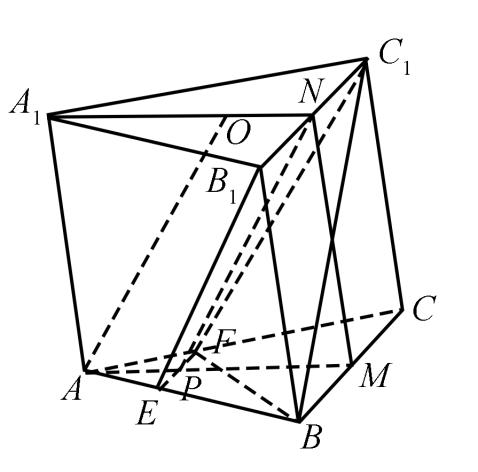
\includegraphics[width=.42\linewidth]{assets/asset-082-01.jpg}
\end{center}
\begin{solution}
\textbf{答案：}（1）证明见解析；（2）24。

\textbf{分析：}（1）由 $M,N$ 分别为 $BC, B_1C_1$ 的中点，$MN\parallel CC_1$，根据条件可得 $AA_1\parallel BB_1$，可证 $MN\parallel AA_1$，要证平面 $EB_1C_1F\perp$ 平面 $A_1AMN$，只需证明 $EF\perp$ 平面 $A_1AMN$ 即可；
（2）根据已知条件求得 $S_{\text{四边形}EB_1C_1F}$ 和 $M$ 到 $PN$ 的距离，根据椎体体积公式，即可求得 $V_{B-EB_1C_1F}$。

\textbf{详解：}（1）$\because M,N$ 分别为 $BC, B_1C_1$ 的中点，$\therefore MN\parallel BB_1$。
又 $AA_1\parallel BB_1$，$\therefore MN\parallel AA_1$。
在等边 $\triangle ABC$ 中，$M$ 为 $BC$ 中点，则 $BC\perp AM$。
$\because$ 侧面 $BB_1C_1C$ 为矩形，$\therefore BC\perp BB_1$。
又 $MN\parallel BB_1$，$\therefore MN\perp BC$。
由 $MN\cap AM=M$，$MN, AM\subset$ 平面 $A_1AMN$，$\therefore BC\perp$ 平面 $A_1AMN$。
又 $B_1C_1\parallel BC$，且 $B_1C_1\not\subset$ 平面 $ABC$，$BC\subset$ 平面 $ABC$，$\therefore B_1C_1\parallel$ 平面 $ABC$。
又 $B_1C_1\subset$ 平面 $EB_1C_1F$，且平面 $EB_1C_1F\cap$ 平面 $ABC=EF$，$\therefore B_1C_1\parallel EF$，$\therefore EF\parallel BC$。
又 $BC\perp$ 平面 $A_1AMN$，$\therefore EF\perp$ 平面 $A_1AMN$。
$\because EF\subset$ 平面 $EB_1C_1F$，$\therefore$ 平面 $EB_1C_1F\perp$ 平面 $A_1AMN$。
（2）过 $M$ 作 $PN$ 的垂线，交点为 $H$。
$\because AO\parallel$ 平面 $EB_1C_1F$，$AO\subset$ 平面 $A_1AMN$，平面 $A_1AMN\cap$ 平面 $EB_1C_1F=NP$，$\therefore AO\parallel NP$。
又 $NO\parallel AP$，$\therefore AO=NP=6$。
$\because O$ 为 $\triangle A_1B_1C_1$ 的中心，$\therefore ON=\frac{1}{3}A_1C_1\sin60^\circ = \frac{1}{3}\times6\times\frac{\sqrt{3}}{2}=\sqrt{3}$。
故 $ON=AP=\sqrt{3}$，则 $AM=3AP=3\sqrt{3}$。
$\because$ 平面 $EB_1C_1F\perp$ 平面 $A_1AMN$，平面 $EB_1C_1F\cap$ 平面 $A_1AMN=NP$，$MH\subset$ 平面 $A_1AMN$，$\therefore MH\perp$ 平面 $EB_1C_1F$。
又 $\because$ 在等边 $\triangle ABC$ 中，$\frac{EF}{BC}=\frac{AP}{AM}$，即 $EF=\frac{AP\cdot BC}{AM}=\frac{\sqrt{3}\times6}{3\sqrt{3}}=2$。
由（1）知，四边形 $EB_1C_1F$ 为梯形，其面积为 $S_{\text{四边形}EB_1C_1F} = \frac{EF+B_1C_1}{2}\cdot NP = \frac{2+6}{2}\times6=24$。
$\because MH = 2\sqrt{3}\cdot\sin60^\circ = 3$，
$\therefore V_{B-EB_1C_1F} = \frac{1}{3}S_{\text{四边形}EB_1C_1F}\cdot MH = \frac{1}{3}\times24\times3=24$。
\end{solution}
\end{question}

\begin{question}[points=5]
\textbf{来源：}2020 年 全国I卷-理科，第 3 题\par
埃及胡夫金字塔是古代世界建筑奇迹之一，它的形状可视为一个正四棱锥。以该四棱锥的高为边长的正方形面积等于该四棱锥一个侧面三角形的面积，则其侧面三角形底边上的高与底面正方形的边长的比值为
\begin{choices}
  \item $\frac{\sqrt{5}-1}{4}$
  \item $\frac{\sqrt{5}-1}{2}$
  \item $\frac{\sqrt{5}+1}{4}$
  \item $\frac{\sqrt{5}+1}{2}$
\end{choices}
\begin{solution}
\textbf{答案：}C

\textbf{详解：}如图，设底面正方形边长为$a$，侧面三角形底边上的高为$b$，则棱锥的高$h=\sqrt{b^2-\left(\frac{a}{2}\right)^2}$。由题意$h^2=\frac{1}{2}ab$，即$b^2-\frac{a^2}{4}=\frac{1}{2}ab$，化简得$4\left(\frac{b}{a}\right)^2-2\cdot\frac{b}{a}-1=0$，解得$\frac{b}{a}=\frac{1+\sqrt{5}}{4}$（负值舍去）。
\end{solution}
\end{question}

\begin{question}[points=5]
\textbf{来源：}2020 年 全国I卷-理科，第 10 题\par
已知$A,B,C$为球$O$的球面上的三个点，$\odot O_1$为$\triangle ABC$的外接圆，若$\odot O_1$的面积为$4\pi$，$AB=BC=AC=OO_1$，则球$O$的表面积为
\begin{choices}
  \item $64\pi$
  \item $48\pi$
  \item $36\pi$
  \item $32\pi$
\end{choices}
\begin{solution}
\textbf{答案：}A

\textbf{详解：}设$\odot O_1$半径为$r$，则$\pi r^2=4\pi$，得$r=2$。由正弦定理$AB=2r\sin60^\circ=2\sqrt{3}$，所以$OO_1=AB=2\sqrt{3}$。又$OO_1\perp$平面$ABC$，$O_1A=r=2$，所以球半径$R=OA=\sqrt{OO_1^2+r^2}=\sqrt{12+4}=4$，球表面积$S=4\pi R^2=64\pi$。
\end{solution}
\end{question}

\begin{question}[points=5]
\textbf{来源：}2020 年 全国I卷-理科，第 16 题；次专题：平面向量与解三角形\par
如图，在三棱锥$P-ABC$的平面展开图中，$AC=1$，$AB=AD=\sqrt{3}$，$AB\perp AC$，$AB\perp AD$，$\angle CAE=30^\circ$，则$\cos\angle FCB=$。

\begin{center}
  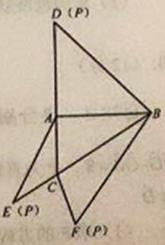
\includegraphics[width=.42\linewidth]{assets/asset-085-01.jpg}
\end{center}
\fillin[{$-\frac{1}{4}$}]
\begin{solution}
\textbf{答案：}$-\frac{1}{4}$

\textbf{详解：}由$AB\perp AC$，$AB=\sqrt{3}$，$AC=1$，由勾股定理得$BC=2$。同理$BD=\sqrt{AB^2+AD^2}=\sqrt{6}$，所以$BF=BD=\sqrt{6}$。在$\triangle ACE$中，$AC=1$，$AE=AD=\sqrt{3}$，$\angle CAE=30^\circ$，由余弦定理得$CE^2=AC^2+AE^2-2AC\cdot AE\cos30^\circ=1+3-2\times1\times\sqrt{3}\times\frac{\sqrt{3}}{2}=1$，所以$CF=CE=1$。在$\triangle BCF$中，$BC=2$，$BF=\sqrt{6}$，$CF=1$，由余弦定理得$\cos\angle FCB=\frac{CF^2+BC^2-BF^2}{2CF\cdot BC}=\frac{1+4-6}{2\times1\times2}=-\frac{1}{4}$。
\end{solution}
\end{question}

\begin{question}[points=12]
\textbf{来源：}2020 年 全国I卷-理科，第 18 题\par
如图，$D$为圆锥的顶点，$O$是圆锥底面的圆心，$AE$为底面直径，$AE=AD$。$\triangle ABC$是底面的内接正三角形，$P$为$DO$上一点，$PO=\frac{\sqrt{6}}{6}DO$。

(1)证明：$PA\perp$平面$PBC$；

(2)求二面角$B-PC-E$的余弦值。

\begin{center}
  
\includegraphics[width=.42\linewidth]{assets/asset-086-01.jpg}
\end{center}
\begin{solution}
\textbf{答案：}(1)证明见解析；(2)$\frac{2\sqrt{5}}{5}$

\textbf{详解：}(1)设$AE=1$，则$DO=\frac{\sqrt{3}}{2}$，$CO=BO=\frac{1}{2}$，$PO=\frac{\sqrt{6}}{6}\times\frac{\sqrt{3}}{2}=\frac{\sqrt{2}}{4}$。计算得$PC=PB=\sqrt{PO^2+OC^2}=\frac{\sqrt{6}}{4}$，$AB=\sqrt{3}OA=\frac{\sqrt{3}}{2}$。由$PA^2+PB^2=AB^2$得$PA\perp PB$，同理$PA\perp PC$，又$PC\cap PB=P$，所以$PA\perp$平面$PBC$。
(2)过$O$作$ON\parallel BC$交$AB$于点$N$，以$O$为原点，$OA$为$x$轴，$ON$为$y$轴建立空间直角坐标系。则$E(-\frac{1}{2},0,0)$，$P(0,0,\frac{\sqrt{2}}{4})$，$B(-\frac{1}{4},\frac{\sqrt{3}}{4},0)$，$C(-\frac{1}{4},-\frac{\sqrt{3}}{4},0)$。
平面$PBC$的一个法向量$\vec{n}=(\sqrt{2},0,-1)$，平面$PCE$的一个法向量$\vec{m}=(1,\frac{\sqrt{3}}{3},-\sqrt{2})$，$\cos\langle\vec{m},\vec{n}\rangle=\frac{\vec{n}\cdot\vec{m}}{|\vec{n}||\vec{m}|}=\frac{2\sqrt{2}}{\sqrt{3}\times\sqrt{\frac{10}{3}}}=\frac{2\sqrt{5}}{5}$。故二面角$B-PC-E$的余弦值为$\frac{2\sqrt{5}}{5}$。
\end{solution}
\end{question}

\begin{question}[points=5]
\textbf{来源：}2020 年 全国I卷-文科，第 3 题\par
埃及胡夫金字塔是古代世界建筑奇迹之一，它的形状可视为一个正四棱锥，以该四棱锥的高为边长的正方形面积等于该四棱锥一个侧面三角形的面积，则其侧面三角形底边上的高与底面正方形的边长的比值为
\begin{choices}
  \item $\frac{\sqrt{5} - 1}{4}$
  \item $\frac{\sqrt{5} - 1}{2}$
  \item $\frac{\sqrt{5} + 1}{4}$
  \item $\frac{\sqrt{5} + 1}{2}$
\end{choices}
\begin{solution}
\textbf{答案：}$\frac{\sqrt{5} + 1}{4}$

\textbf{分析：}设 $CD = a$, $PE = b$, 利用 $PO^2 = \frac{1}{2} CD \cdot PE$ 得到关于 $a, b$ 的方程，解方程即可得到答案.

\textbf{详解：}如图，设 $CD = a$, $PE = b$, 则 $PO = \sqrt{PE^2 - OE^2} = \sqrt{b^2 - \frac{a^2}{4}}$. 由题意 $PO^2 = \frac{1}{2} ab$, 即 $b^2 - \frac{a^2}{4} = \frac{1}{2} ab$, 化简得 $4\left(\frac{b}{a}\right)^2 - 2\cdot \frac{b}{a} - 1 = 0$, 解得 $\frac{b}{a} = \frac{1+\sqrt{5}}{4}$ (负值舍去). 故选C.
\end{solution}
\end{question}

\begin{question}[points=5]
\textbf{来源：}2020 年 全国I卷-文科，第 12 题\par
已知 $A, B, C$ 为球 $O$ 的球面上的三个点，$\odot O_1$ 为 $\triangle ABC$ 的外接圆，若 $\odot O_1$ 的面积为 $4\pi$, $AB = BC = AC = OO_1$, 则球 $O$ 的表面积为
\begin{choices}
  \item $64\pi$
  \item $48\pi$
  \item $36\pi$
  \item $32\pi$
\end{choices}
\begin{solution}
\textbf{答案：}$64\pi$

\textbf{分析：}由已知可得等边 $\triangle ABC$ 的外接圆半径，进而求出其边长，得出 $OO_1$ 的值，根据球截面性质，求出球的半径，即可得出结论.

\textbf{详解：}设圆 $O_1$ 半径为 $r$, 球的半径为 $R$, 依题意得 $\pi r^2 = 4\pi$, 所以 $r=2$. 由正弦定理可得 $AB = 2r\sin 60^\circ = 2\sqrt{3}$, 所以 $OO_1 = AB = 2\sqrt{3}$. 根据圆截面性质 $OO_1 \perp$ 平面 $ABC$, 所以 $OO_1 \perp O_1A$, $R = OA = \sqrt{OO_1^2 + O_1A^2} = \sqrt{(2\sqrt{3})^2 + 2^2} = 4$, 所以球 $O$ 的表面积 $S = 4\pi R^2 = 64\pi$.
\end{solution}
\end{question}

\begin{question}[points=12]
\textbf{来源：}2020 年 全国I卷-文科，第 19 题\par
如图，$D$ 为圆锥的顶点，$O$ 是圆锥底面的圆心，$\triangle ABC$ 是底面的内接正三角形，$P$ 为 $DO$ 上一点，$\angle APC = 90^\circ$.



(1) 证明：平面 $PAB \perp$ 平面 $PAC$;



(2) 设 $DO = \sqrt{2}$, 圆锥的侧面积为 $\sqrt{3}\pi$, 求三棱锥 $P-ABC$ 的体积.

\begin{center}
  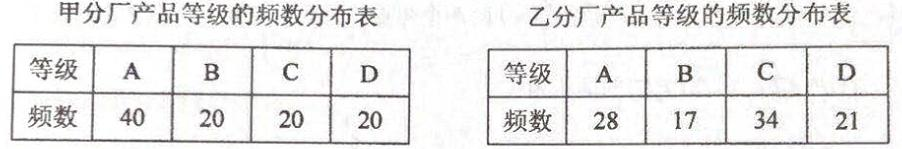
\includegraphics[width=.42\linewidth]{assets/asset-089-01.jpg}
\end{center}
\begin{solution}
\textbf{答案：}(1) 证明见解析; (2) $\frac{\sqrt{6}}{8}$.

\textbf{分析：}(1) 根据已知可得 $PA=PB=PC$, 进而有 $\triangle PAC \cong \triangle PBC$, 可得 $\angle APC = \angle BPC = 90^\circ$, 即 $PB \perp PC$, 从而证得 $PC \perp$ 平面 $PAB$, 即可证得结论； (2) 将已知条件转化为母线 $l$ 和底面半径 $r$ 的关系，进而求出底面半径，由正弦定理，求出正三角形 $ABC$ 边长，在等腰直角三角形 $APC$ 中求出 $AP$, 在 $\triangle APO$ 中求出 $PO$, 即可求出结论.

\textbf{详解：}(1) 因为 $D$ 为圆锥顶点，$O$ 为底面圆心，所以 $OD \perp$ 平面 $ABC$. 因为 $P$ 在 $DO$ 上，$OA = OB = OC$, 所以 $PA = PB = PC$. 又 $\triangle ABC$ 是圆内接正三角形，所以 $AC = BC$, 故 $\triangle PAC \cong \triangle PBC$, 所以 $\angle APC = \angle BPC = 90^\circ$, 即 $PB \perp PC$, $PA \perp PC$. 因为 $PA \cap PB = P$, 所以 $PC \perp$ 平面 $PAB$, 又 $PC \subset$ 平面 $PAC$, 所以平面 $PAB \perp$ 平面 $PAC$.

(2) 设圆锥的母线为 $l$, 底面半径为 $r$, 圆锥的侧面积为 $\pi rl = \sqrt{3}\pi$, 所以 $rl = \sqrt{3}$. 又 $OD^2 = l^2 - r^2 = 2$, 解得 $r=1$, $l=\sqrt{3}$. 正三角形 $ABC$ 的边长 $AC = 2r\sin60^\circ = \sqrt{3}$. 在等腰直角三角形 $APC$ 中，$AP = \frac{\sqrt{2}}{2} AC = \frac{\sqrt{6}}{2}$. 在 $\triangle APO$ 中，$PO = \sqrt{AP^2 - OA^2} = \sqrt{\frac{6}{4} - 1} = \frac{\sqrt{2}}{2}$. 所以三棱锥 $P-ABC$ 的体积 $V_{P-ABC} = \frac{1}{3} PO \cdot S_{\triangle ABC} = \frac{1}{3} \times \frac{\sqrt{2}}{2} \times \frac{\sqrt{3}}{4} \times \sqrt{3} = \frac{\sqrt{6}}{8}$.
\end{solution}
\end{question}

\section*{2021 年}

\begin{question}[points=4]
\textbf{来源：}2021 年 北京卷，第 4 题\par
某四面体的三视图如图所示, 该四面体的表面积为（ ）

\begin{center}
  
\includegraphics[width=.42\linewidth]{assets/asset-090-01.jpg}
\end{center}
\begin{choices}
  \item $\frac{3+\sqrt{3}}{2}$
  \item $4$
  \item $3+\sqrt{3}$
  \item $2$
\end{choices}
\begin{solution}
\textbf{答案：}A

\textbf{分析：}根据三视图可得如图所示的几何体（三棱锥）, 根据三视图中的数据可计算该几何体的表面积.

\textbf{详解：}根据三视图可得如图所示的几何体-正三棱锥 $O-ABC$, 其侧面为等腰直角三角形, 底面等边三角形, 由三视图可得该正三棱锥的侧棱长为 $1$, 故其表面积为 $3\times\frac{1}{2}\times1\times1+\frac{\sqrt{3}}{4}\times(\sqrt{2})^2=\frac{3+\sqrt{3}}{2}$.
\end{solution}
\end{question}

\begin{question}[points=4]
\textbf{来源：}2021 年 北京卷，第 8 题\par
定义: 24小时内降水在平地上积水厚度（mm）来判断降雨程度. 其中小雨（$<10$ mm）, 中雨（$10$ mm $-25$ mm）, 大雨（$25$ mm $-50$ mm）, 暴雨（$50$ mm $-100$ mm）. 小明用一个圆锥形容器接了24小时的雨水, 如图, 则这天降雨属于哪个等级（ ）

\begin{center}
  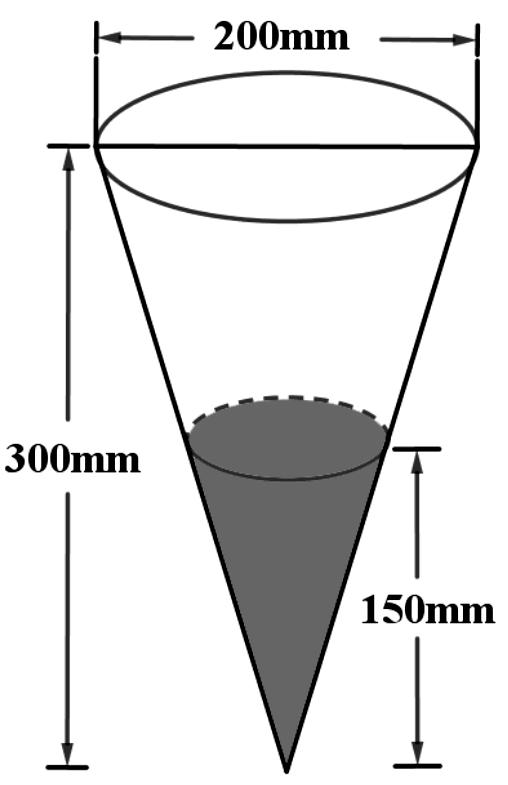
\includegraphics[width=.42\linewidth]{assets/asset-091-01.jpg}
\end{center}
\begin{choices}
  \item 小雨
  \item 中雨
  \item 大雨
  \item 暴雨
\end{choices}
\begin{solution}
\textbf{答案：}B

\textbf{分析：}计算出圆锥体积, 除以圆面的面积即可得降雨量, 即可得解.

\textbf{详解：}由题意, 一个半径为 $\frac{200}{2}=100$ mm 的圆面内的降雨充满一个底面半径为 $\frac{200}{2}\times\frac{150}{300}=50$ mm, 高为 $150$ mm 的圆锥, 所以积水厚度 $d=\frac{\frac{1}{3}\pi\times 50^2 \times 150}{\pi\times 100^2}=12.5$ mm, 属于中雨.
\end{solution}
\end{question}

\begin{question}[points=14]
\textbf{来源：}2021 年 北京卷，第 17 题\par
已知正方体 $ABCD-A_1B_1C_1D_1$, 点 $E$ 为 $A_1D_1$ 中点, 直线 $B_1C_1$ 交平面 $CDE$ 于点 $F$.

(1) 证明: 点 $F$ 为 $B_1C_1$ 的中点;

(2) 若点 $M$ 为棱 $A_1B_1$ 上一点, 且二面角 $M-CF-E$ 的余弦值为 $\frac{\sqrt{5}}{3}$, 求 $\frac{A_1M}{A_1B_1}$ 的值.
\begin{solution}
\textbf{答案：}(1) 证明见解析; (2) $\frac{A_1M}{A_1B_1}=\frac{1}{2}$.

\textbf{分析：}(1) 将平面 $CDE$ 扩展, 结合所得平面与直线 $B_1C_1$ 的交点即可证得; (2) 建立空间直角坐标系, 利用向量法求解.

\textbf{详解：}(1) 取 $B_1C_1$ 的中点 $F'$, 连接 $DE, EF', F'C$, 由正方体性质, $E,F'$ 为中点, 故 $EF'\parallel CD$, 从而 $E,F',C,D$ 四点共面, 即平面 $CDE$ 即平面 $CDEF'$, 所以直线 $B_1C_1$ 交平面 $CDE$ 于点 $F'$, 由直线与平面相交唯一交点, 故点 $F$ 与点 $F'$ 重合, 即点 $F$ 为 $B_1C_1$ 中点.
(2) 以点 $D$ 为原点, $DA, DC, DD_1$ 方向为 $x,y,z$ 轴建立空间直角坐标系, 设正方体棱长为 $2$, 设 $\frac{A_1M}{A_1B_1}=\lambda(0\leq\lambda\leq1)$, 则 $M(2,2\lambda,2), C(0,2,0), F(1,2,2), E(1,0,2)$. 则 $\overrightarrow{MC}=(-2,2-2\lambda,-2)$, $\overrightarrow{CF}=(1,0,2)$, $\overrightarrow{FE}=(0,-2,0)$. 设平面 $MCF$ 的法向量 $\vec{m}=(x_1,y_1,z_1)$, 由 $\begin{cases} \vec{m}\cdot\overrightarrow{MC}=-2x_1+(2-2\lambda)y_1-2z_1=0 \\ \vec{m}\cdot\overrightarrow{CF}=x_1+2z_1=0 \end{cases}$, 令 $z_1=-1$, 得 $\vec{m}=(2,\frac{1}{1-\lambda},-1)$. 设平面 $CFE$ 的法向量 $\vec{n}=(x_2,y_2,z_2)$, 由 $\begin{cases} \vec{n}\cdot\overrightarrow{FE}=-2y_2=0 \\ \vec{n}\cdot\overrightarrow{CF}=x_2+2z_2=0 \end{cases}$, 令 $z_2=-1$, 得 $\vec{n}=(2,0,-1)$. 则 $\cos\langle\vec{m},\vec{n}\rangle=\frac{\vec{m}\cdot\vec{n}}{|\vec{m}||\vec{n}|}=\frac{5}{\sqrt{5+(\frac{1}{1-\lambda})^2}\cdot\sqrt{5}}=\frac{\sqrt{5}}{3}$, 解得 $(\lambda-1)^2=\frac{1}{4}$, 故 $\lambda=\frac{1}{2}$ (舍去 $\frac{3}{2}$). 所以 $\frac{A_1M}{A_1B_1}=\frac{1}{2}$.
\end{solution}
\end{question}

\begin{question}[points=5]
\textbf{来源：}2021 年 全国甲卷-理科，第 6 题\par
在一个正方体中，过顶点 $A$ 的三条棱的中点分别为 $E, F, G$．该正方体截去三棱锥 $A-EFG$ 后，所得多面体的三视图中，正视图如图所示，则相应的侧视图是（ ）

\begin{center}
  
\includegraphics[width=.42\linewidth]{assets/asset-093-01.jpg}
\end{center}
\begin{choices}
  \item 
  \item 
  \item 
  \item 
\end{choices}
\begin{solution}
\textbf{答案：}D

\textbf{分析：}根据题意及题目所给的正视图还原出几何体的直观图，结合直观图进行判断．

\textbf{详解：}由题意及正视图可得几何体的直观图，如图所示，所以其侧视图为D．
\end{solution}
\end{question}

\begin{question}[points=5]
\textbf{来源：}2021 年 全国甲卷-理科，第 11 题\par
已知 $A, B, C$ 是半径为1的球 $O$ 的球面上的三个点，且 $AC \perp BC$, $AC = BC = 1$，则三棱锥 $O-ABC$ 的体积为（ ）
\begin{choices}
  \item $\frac{\sqrt{2}}{12}$
  \item $\frac{\sqrt{3}}{12}$
  \item $\frac{\sqrt{2}}{4}$
  \item $\frac{\sqrt{3}}{4}$
\end{choices}
\begin{solution}
\textbf{答案：}A

\textbf{分析：}由题可得 $\triangle ABC$ 为等腰直角三角形，得出 $\triangle ABC$ 外接圆的半径，则可求得 $O$ 到平面 $ABC$ 的距离，进而求得体积．

\textbf{详解：}因为 $AC \perp BC$, $AC = BC = 1$，所以 $AB = \sqrt{2}$，$\triangle ABC$ 外接圆半径 $r = \frac{\sqrt{2}}{2}$．球半径 $R=1$，则 $O$ 到平面 $ABC$ 的距离 $d = \sqrt{1^2 - \left(\frac{\sqrt{2}}{2}\right)^2} = \frac{\sqrt{2}}{2}$，故 $V_{O-ABC} = \frac{1}{3} \cdot \frac{1}{2} \cdot 1 \cdot 1 \cdot \frac{\sqrt{2}}{2} = \frac{\sqrt{2}}{12}$．
\end{solution}
\end{question}

\begin{question}[points=12]
\textbf{来源：}2021 年 全国甲卷-理科，第 19 题\par
已知直三棱柱 $ABC-A_1B_1C_1$ 中，侧面 $AA_1B_1B$ 为正方形，$AB=BC=2$，$E, F$ 分别为 $AC$ 和 $CC_1$ 的中点，$D$ 为棱 $A_1B_1$ 上的点，$BF \perp A_1B_1$．（1）证明：$BF \perp DE$；（2）当 $B_1D$ 为何值时，面 $BB_1C_1C$ 与面 $DFE$ 所成的二面角的正弦值最小？
\begin{solution}
\textbf{答案：}（1）见解析；（2）$B_1D = \frac{1}{2}$

\textbf{分析：}通过已知条件，确定三条互相垂直的直线，建立合适的空间直角坐标系，借助空间向量证明线线垂直和求出二面角的平面角的余弦值最大，进而可以确定出答案．

\textbf{详解：}（1）因为直三棱柱，$BB_1 \perp$ 底面 $ABC$，所以 $BB_1 \perp AB$．又 $A_1B_1 \parallel AB$，$BF \perp A_1B_1$，所以 $BF \perp AB$，故 $AB \perp$ 平面 $BCC_1B_1$．以 $B$ 为原点，$BA, BC, BB_1$ 为 $x, y, z$ 轴建立空间直角坐标系，则 $B(0,0,0), A(2,0,0), C(0,2,0), B_1(0,0,2), A_1(2,0,2), C_1(0,2,2), E(1,1,0), F(0,2,1)$．设 $D(a,0,2)$（$0\le a\le 2$），则 $\overrightarrow{BF}=(0,2,1)$，$\overrightarrow{DE}=(1-a,1,-2)$，$\overrightarrow{BF}\cdot\overrightarrow{DE}=0$，故 $BF \perp DE$．（2）平面 $DFE$ 的法向量 $\vec{m}=(3,1+a,2-a)$，平面 $BCC_1B_1$ 的法向量 $\overrightarrow{BA}=(2,0,0)$，二面角的余弦值 $\cos\theta = \frac{|\vec{m}\cdot\overrightarrow{BA}|}{|\vec{m}||\overrightarrow{BA}|} = \frac{6}{2\sqrt{2a^2-2a+14}} = \frac{3}{\sqrt{2a^2-2a+14}}$，当 $a=\frac{1}{2}$ 时，分母最小，$\cos\theta$ 最大，$\sin\theta$ 最小，此时 $B_1D = a = \frac{1}{2}$．
\end{solution}
\end{question}

\begin{question}[points=5]
\textbf{来源：}2021 年 全国甲卷-文科，第 7 题\par
在一个正方体中，过顶点 $A$ 的三条棱的中点分别为 $E, F, G$．该正方体截去三棱锥 $A-EFG$ 后，所得多面体的三视图中，正视图如图所示，则相应的侧视图是（ ）

\begin{center}
  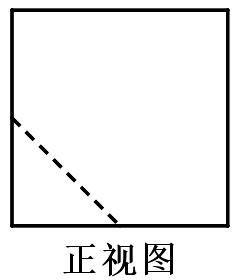
\includegraphics[width=.42\linewidth]{assets/asset-096-01.jpg}
\end{center}

\begin{center}
  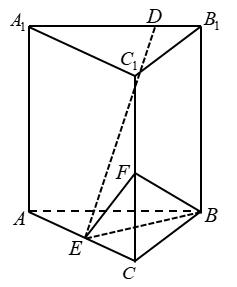
\includegraphics[width=.42\linewidth]{assets/asset-096-02.jpg}
\end{center}
\begin{choices}
  \item 
  \item 
  \item 
  \item 
\end{choices}
\begin{solution}
\textbf{答案：}D

\textbf{分析：}根据题意及题目所给的正视图还原出几何体的直观图，结合直观图进行判断.

\textbf{详解：}由题意及正视图可得几何体的直观图，如图所示，

所以其侧视图为

故选：D.
\end{solution}
\end{question}

\begin{question}[points=5]
\textbf{来源：}2021 年 全国甲卷-文科，第 14 题\par
已知一个圆锥的底面半径为6，其体积为 $30\pi$ 则该圆锥的侧面积为.
\fillin[{$39\pi$}]
\begin{solution}
\textbf{答案：}$39\pi$

\textbf{分析：}利用体积公式求出圆锥的高，进一步求出母线长，最终利用侧面积公式求出答案.

\textbf{详解：}因为 $V = \frac{1}{3}\pi \cdot 6^2 \cdot h = 30\pi$, 所以 $h = \frac{5}{2}$. 所以 $l = \sqrt{h^2 + r^2} = \sqrt{\left(\frac{5}{2}\right)^2 + 6^2} = \frac{13}{2}$. 所以 $S_{\text{侧}} = \pi r l = \pi \times 6 \times \frac{13}{2} = 39\pi$.
\end{solution}
\end{question}

\begin{question}[points=12]
\textbf{来源：}2021 年 全国甲卷-文科，第 19 题\par
已知直三棱柱 $ABC-A_1B_1C_1$ 中，侧面 $AA_1B_1B$ 为正方形，$AB=BC=2$, $E, F$ 分别为 $AC$ 和 $CC_1$ 的中点，$BF \perp A_1B_1$.



（1）求三棱锥 $F-EBC$ 的体积；



（2）已知 $D$ 为棱 $A_1B_1$ 上的点，证明：$BF \perp DE$.
\begin{solution}
\textbf{答案：}(1) $\frac{1}{3}$；(2)证明见解析.

\textbf{分析：}(1)首先求得 $AC$ 的长度，然后利用体积公式可得三棱锥的体积；(2)将所给的几何体进行补形，从而把线线垂直的问题转化为证明线面垂直，然后再由线面垂直可得题中的结论.

\textbf{详解：}(1)如图所示，连结 $AF$. 由题意可得：$BF = \sqrt{BC^2 + CF^2} = \sqrt{4+1} = \sqrt{5}$. 由于 $AB \perp BB_1$, $BC \perp AB$, $BB_1 \cap BC = B$, 故 $AB \perp$ 平面 $BCC_1B_1$, 而 $BF \subset$ 平面 $BCC_1B_1$, 故 $AB \perp BF$, 从而有 $AF = \sqrt{AB^2 + BF^2} = \sqrt{4+5} = 3$, 从而 $AC = \sqrt{AF^2 - CF^2} = \sqrt{9-1} = 2\sqrt{2}$, 则 $AB^2 + BC^2 = AC^2$, 所以 $AB \perp BC$, $\triangle ABC$ 为等腰直角三角形. $S_{\triangle BCE} = \frac{1}{2} S_{\triangle ABC} = \frac{1}{2} \times \frac{1}{2} \times 2 \times 2 = 1$, $V_{F-EBC} = \frac{1}{3} S_{\triangle BCE} \times CF = \frac{1}{3} \times 1 \times 1 = \frac{1}{3}$.

(2)由(1)的结论可将几何体补形为一个棱长为2的正方体 $ABCM-A_1B_1C_1M_1$, 如图所示，取棱 $AM, BC$ 的中点 $H, G$, 连结 $A_1H, HG, GB_1$. 正方形 $BCC_1B_1$ 中, $G, F$ 为中点, 则 $BF \perp B_1G$, 又 $BF \perp A_1B_1$, $A_1B_1 \cap B_1G = B_1$, 故 $BF \perp$ 平面 $A_1B_1GH$, 而 $DE \subset$ 平面 $A_1B_1GH$, 从而 $BF \perp DE$.
\end{solution}
\end{question}

\begin{question}[points=5]
\textbf{来源：}2021 年 全国乙卷-理科，第 5 题\par
在正方体$ABCD-A_1B_1C_1D_1$中，$P$为$B_1D_1$的中点，则直线$PB$与$AD_1$所成的角为（  ）
\begin{choices}
  \item $\frac{\pi}{2}$
  \item $\frac{\pi}{3}$
  \item $\frac{\pi}{4}$
  \item $\frac{\pi}{6}$
\end{choices}
\begin{solution}
\textbf{答案：}$\frac{\pi}{6}$

\textbf{详解：}如图，$\angle PBC_1$为直线$PB$与$AD_1$所成角的平面角。易知$\triangle A_1B_1C_1$为正三角形，又$P$为$A_1C_1$中点，所以$\angle PBC_1=\frac{\pi}{6}$。故选D。
\end{solution}
\end{question}

\begin{question}[points=5]
\textbf{来源：}2021 年 全国乙卷-理科，第 16 题\par
以图①为正视图，在图②③④⑤中选两个分别作为侧视图和俯视图，组成某个三棱锥的三视图，则所选侧视图和俯视图的编号依次为（写出符合要求的一组答案即可）。

\begin{center}
  
\includegraphics[width=.42\linewidth]{assets/asset-100-01.jpg}
\end{center}
\fillin[{$②⑤或③④$}]
\begin{solution}
\textbf{答案：}$②⑤或③④$

\textbf{详解：}由高度可知，侧视图只能为②或③。侧视图为②，如图（1），平面$PAC\perp$平面$ABC$，$PA=PC=\sqrt{2}$，$BA=BC=\sqrt{5}$，$AC=2$，俯视图为⑤。俯视图为③，如图（2），$PA\perp$平面$ABC$，$PA=1$，$AC=AB=\sqrt{5}$，$BC=2$，俯视图为④。
\end{solution}
\end{question}

\begin{question}[points=12]
\textbf{来源：}2021 年 全国乙卷-理科，第 18 题\par
如图，四棱锥$P-ABCD$的底面是矩形，$PD\perp$底面$ABCD$，$PD=DC=1$，$M$为$BC$的中点，且$PB\perp AM$。

（1）求$BC$；

（2）求二面角$A-PM-B$的正弦值。

\begin{center}
  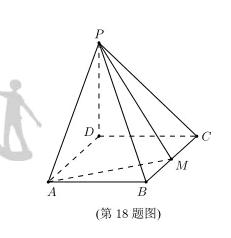
\includegraphics[width=.42\linewidth]{assets/asset-101-01.jpg}
\end{center}
\begin{solution}
\textbf{答案：}（1）$\sqrt{2}$；（2）$\frac{\sqrt{70}}{14}$

\textbf{详解：}（1）因为$PD\perp$平面$ABCD$，且矩形$ABCD$中，$AD\perp DC$。所以以$\overrightarrow{DA}$，$\overrightarrow{DC}$，$\overrightarrow{DP}$分别为$x$，$y$，$z$轴正方向，$D$为原点建立空间直角坐标系$D-xyz$。设$BC=t$，$A(t,0,0)$，$B(t,1,0)$，$M(\frac{t}{2},1,0)$，$P(0,0,1)$，所以$\overrightarrow{PB}=(t,1,-1)$，$\overrightarrow{AM}=(-\frac{t}{2},1,0)$。因为$PB\perp AM$，所以$\overrightarrow{PB}\cdot\overrightarrow{AM}=-\frac{t^2}{2}+1=0$，所以$t=\sqrt{2}$，所以$BC=\sqrt{2}$。
（2）设平面$APM$的一个法向量为$\vec{m}=(x,y,z)$，由于$\overrightarrow{AP}=(-\sqrt{2},0,1)$，则$\begin{cases} \vec{m}\cdot\overrightarrow{AP}=-\sqrt{2}x+z=0 \\ \vec{m}\cdot\overrightarrow{AM}=-\frac{\sqrt{2}}{2}x+y=0 \end{cases}$。令$x=\sqrt{2}$，得$\vec{m}=(\sqrt{2},1,2)$。设平面$PMB$的一个法向量为$\vec{n}=(x',y',z')$，则$\begin{cases} \vec{n}\cdot\overrightarrow{CB}=\sqrt{2}x'=0 \\ \vec{n}\cdot\overrightarrow{PB}=\sqrt{2}x'+y'-z'=0 \end{cases}$。令$y'=1$，得$\vec{n}=(0,1,1)$。所以$\cos\langle\vec{m},\vec{n}\rangle=\frac{\vec{m}\cdot\vec{n}}{|\vec{m}||\vec{n}|}=\frac{3}{\sqrt{7}\times\sqrt{2}}=\frac{3\sqrt{14}}{14}$，所以二面角$A-PM-B$的正弦值为$\frac{\sqrt{70}}{14}$。
\end{solution}
\end{question}

\begin{question}[points=5]
\textbf{来源：}2021 年 全国乙卷-文科，第 10 题\par
在正方体 $ABCD-A_1B_1C_1D_1$ 中，$P$ 为 $B_1D_1$ 的中点，则直线 $PB$ 与 $AD_1$ 所成的角为（ ）
\begin{choices}
  \item $\frac{\pi}{2}$
  \item $\frac{\pi}{3}$
  \item $\frac{\pi}{4}$
  \item $\frac{\pi}{6}$
\end{choices}
\begin{solution}
\textbf{答案：}D

\textbf{分析：}做出图形，$AD_1 // BC_1$ ，所以 $\angle PBC_1$ 为异面直线所成角，设棱长为1.
$BC_1 = \sqrt{2}$ ，$B_1P = \frac{\sqrt{2}}{2}$ ，$PC_1 = \frac{\sqrt{2}}{2}$ ，$BP = \frac{\sqrt{6}}{2}$ .
$\cos\angle PBC_1 = \frac{BC_1^2 + BP^2 - C_1P^2}{2\cdot BP \cdot BC_1} = \frac{2 + \frac{3}{2} - \frac{1}{2}}{2\cdot\frac{\sqrt{6}}{2}\cdot\sqrt{2}} = \frac{3}{\sqrt{12}} = \frac{\sqrt{3}}{2}$ ，即 $\angle PBC_1 = \frac{\pi}{6}$ ，故选 D.
\end{solution}
\end{question}

\begin{question}[points=5]
\textbf{来源：}2021 年 全国乙卷-文科，第 16 题\par
以图①为正视图，在图②③④⑤中选两个分别作为侧视图和俯视图，组成某个三棱锥的三视图，则所选侧视图和俯视图的编号依次为 （写出符合要求的一组答案即可）.

\begin{center}
  
\includegraphics[width=.42\linewidth]{assets/asset-103-01.jpg}
\end{center}
\fillin[{$②⑤或③④$}]
\begin{solution}
\textbf{答案：}$②⑤或③④$

\textbf{分析：}由高度可知，侧视图只能为②或③.
侧视图为②，如图（1），平面 $PAC \perp$ 平面 $ABC$ ， $PA = PC = \sqrt{2}$ ， $BA = BC = \sqrt{5}$ ， $AC = 2$ ，俯视图为⑤.
俯视图为③，如图（2）， $PA \perp$ 平面 $ABC$ ， $PA = 1$ ， $AC = AB = \sqrt{5}$ ， $BC = 2$ ，俯视图为④.
\end{solution}
\end{question}

\begin{question}[points=12]
\textbf{来源：}2021 年 全国乙卷-文科，第 18 题\par
如图，四棱锥 $P-ABCD$ 的底面是矩形， $PD \perp$ 底面 $ABCD$ ， $M$ 为 $BC$ 的中点，且 $PB \perp AM$ .

（1）证明：平面 $PAM \perp$ 平面 $PBD$ ﹔

（2）若 $PD = DC = 1$ ，求四棱锥 $P-ABCD$ 的体积.
\begin{solution}
\textbf{答案：}见解析

\textbf{详解：}（1）证明：因为 $PD \perp$ 底面 $ABCD$ ， $AM \subset$ 底面 $ABCD$ ，所以 $PD \perp AM$ .
又 $PB \perp AM$ ， $PD \cap PB = P$ ， $PD, PB \subset$ 平面 $PBD$ ，所以 $AM \perp$ 平面 $PBD$ .
又 $AM \subset$ 平面 $PAM$ ，所以平面 $PAM \perp$ 平面 $PBD$ .
（2）设 $AB = DC = 1$ ， $BC = AD = a$ ，则 $M$ 为 $BC$ 中点，$BM = \frac{a}{2}$ .
在 $\triangle AMB$ 中，$AM^2 = AB^2 + BM^2 = 1 + \frac{a^2}{4}$ .
在 $\triangle PBD$ 中，$PB^2 = PD^2 + DB^2 = 1 + (1+a^2) = a^2+2$ .
因为 $PB \perp AM$ ，所以 $PB^2 + AM^2 = PA^2$ （？）实际上，需用其他方法.
\end{solution}
\end{question}

\begin{question}[points=4]
\textbf{来源：}2021 年 上海春季卷，第 3 题\par
已知圆柱的底面半径为1，高为2，则圆柱的侧面积为  .
\fillin[{$4\pi$}]
\begin{solution}
\textbf{答案：}$4\pi$

\textbf{分析：}根据圆柱的侧面积公式计算即可．

\textbf{详解：}圆柱的底面半径为 $r=1$，高为 $h=2$，所以圆柱的侧面积为 $S_{\text{侧}}=2\pi rh=2\pi\times 1\times 2=4\pi$．
\end{solution}
\end{question}

\begin{question}[points=14]
\textbf{来源：}2021 年 上海春季卷，第 17 题\par
四棱锥 $P-ABCD$，底面为正方形 $ABCD$，边长为4，$E$ 为 $AB$ 中点，$PE\perp$ 平面 $ABCD$．\begin{enumerate}\item[(1)] 若 $\triangle PAB$ 为等边三角形，求四棱锥 $P-ABCD$ 的体积；\item[(2)] 若 $CD$ 的中点为 $F$，$PF$ 与平面 $ABCD$ 所成角为 $45^\circ$，求 $PC$ 与 $AD$ 所成角的大小．\end{enumerate}
\begin{solution}
\textbf{答案：}$(1)\ \frac{32\sqrt{3}}{3}$；$(2)\ \arctan\frac{\sqrt{5}}{2}$

\textbf{分析：}（1）由 $V=\frac{1}{3}PE\cdot S_{\text{正方形}ABCD}$，代入相应数据，进行运算，即可；\newline（2）由 $PE\perp$ 平面 $ABCD$，知 $\angle PFE=45^\circ$，进而有 $PE=FE=4$，$PB=2\sqrt{5}$，由 $AD//BC$，知 $\angle PCB$ 或其补角即为所求，可证 $BC\perp$ 平面 $PAB$，从而有 $BC\perp PB$，最后在 $\text{Rt}\triangle PBC$ 中，由 $\tan\angle PCB=\frac{PB}{BC}$，得解．

\textbf{详解：}（1）因为 $\triangle PAB$ 为等边三角形，且 $E$ 为 $AB$ 中点，$AB=4$，所以 $PE=2\sqrt{3}$，又 $PE\perp$ 平面 $ABCD$，所以四棱锥 $P-ABCD$ 的体积 $V=\frac{1}{3}PE\cdot S_{\text{正方形}ABCD}=\frac{1}{3}\times 2\sqrt{3}\times 4^2=\frac{32\sqrt{3}}{3}$．\newline（2）因为 $PE\perp$ 平面 $ABCD$，所以 $\angle PFE$ 为 $PF$ 与平面 $ABCD$ 所成角为 $45^\circ$，即 $\angle PFE=45^\circ$，所以 $\triangle PEF$ 为等腰直角三角形，因为 $E$，$F$ 分别为 $AB$，$CD$ 的中点，所以 $PE=FE=4$，所以 $PB=\sqrt{PE^2+BE^2}=2\sqrt{5}$，因为 $AD//BC$，所以 $\angle PCB$ 或其补角即为 $PC$ 与 $AD$ 所成角，因为 $PE\perp$ 平面 $ABCD$，所以 $PE\perp BC$，又 $BC\perp AB$，$PE\cap AB=E$，$PE$、$AB\subset$ 平面 $PAB$，所以 $BC\perp$ 平面 $PAB$，所以 $BC\perp PB$，在 $\text{Rt}\triangle PBC$ 中，$\tan\angle PCB=\frac{PB}{BC}=\frac{2\sqrt{5}}{4}=\frac{\sqrt{5}}{2}$，故 $PC$ 与 $AD$ 所成角的大小为 $\arctan\frac{\sqrt{5}}{2}$．
\end{solution}
\end{question}

\begin{question}[points=5]
\textbf{来源：}2021 年 上海卷，第 9 题\par
在圆柱底面半径为1,高为2, $AB$为上底底面的直径,点$C$是下底底面圆弧上的一个动点，点$C$绕着下底底面旋转一周，则$\triangle ABC$面积的范围．
\fillin[{$[2,\sqrt{5}]$}]
\begin{solution}
\textbf{答案：}$[2,\sqrt{5}]$

\textbf{分析：}注意几何题设与几何性质选择求$\triangle ABC$面积的的方法；

\textbf{详解：}由题意，当点$C$在下底底面圆弧上的运动时，$\triangle ABC$的底边$AB=2$，所以，$\triangle ABC$面积的取值与高$C_2O_1$相关；当$C_2O_1\perp A_1C_1$时，$C_2O_1$最大为：$C_2O_1=\sqrt{1^2+2^2}=\sqrt{5}$，$\triangle ABC$面积的最大值为：$\frac{1}{2}\times2\times\sqrt{5}=\sqrt{5}$；当$AB\perp BC_1$时，$C_2O_1$最小为：$BC_1=2$，$\triangle ABC$面积的最小值为：$\frac{1}{2}\times2\times2=2$；所以，$\triangle ABC$面积的取值范围为：$[2,\sqrt{5}]$
\end{solution}
\end{question}

\begin{question}[points=14]
\textbf{来源：}2021 年 上海卷，第 17 题\par
如图，在长方体$ABCD-A_1B_1C_1D_1$中，$AB=BC=2, AA_1=3$（1）若$P$是边$A_1D_1$的动点，求三棱锥$P-ADC$的体积；（2）求$AB_1$与平面$ACC_1A_1$所成的角的大小.
\begin{solution}
\textbf{答案：}(1)$2$；(2)$\arcsin\frac{\sqrt{26}}{13}$

\textbf{分析：}（1)利用体积计算公式计算；（2）证明$OB_1\perp$平面$ACC_1A_1$，找到线面角度，再计算

\textbf{详解：}（1)如图1，$V_{P-ADC}=\frac{1}{3}S_{\triangle ADC}\times h=\frac{1}{3}\times\frac{1}{2}\times2\times2\times3=2$；（2）如图2，$\because OB_1\perp A_1C_1$, $OB_1\perp OO_1\Rightarrow OB_1\perp$平面$ACC_1A_1\Rightarrow \theta=\angle B_1AO_1$为$AB_1$与平面$ACC_1A_1$所成的角；在$Rt\triangle B_1AO_1$中$B_1O_1=\sqrt{2}$, $AB_1=\sqrt{13}$, $\sin\theta=\frac{B_1O_1}{AB_1}=\frac{\sqrt{2}}{\sqrt{13}}=\frac{\sqrt{26}}{13}$, $\theta=\arcsin\frac{\sqrt{26}}{13}$
\end{solution}
\end{question}

\begin{question}[points=5]
\textbf{来源：}2021 年 天津卷，第 6 题\par
两个圆锥的底面是一个球的同一截面，顶点均在球面上，若球的体积为 $\frac{32\pi}{3}$，两个圆锥的高之比为 $1:3$，则这两个圆锥的体积之和为（   ）

\begin{center}
  
\includegraphics[width=.42\linewidth]{assets/asset-109-01.jpg}
\end{center}
\begin{choices}
  \item $3\pi$
  \item $4\pi$
  \item $9\pi$
  \item $12\pi$
\end{choices}
\begin{solution}
\textbf{答案：}B

\textbf{分析：}作出图形，计算球体的半径，可计算得出两圆锥的高，利用三角形相似计算出圆锥的底面圆半径，再利用锥体体积公式可求得结果.

\textbf{详解：}设球半径为 $R$，则 $\frac{4\pi R^3}{3} = \frac{32\pi}{3}$，得 $R=2$，所以 $AB=4$，设圆锥高之比为 $1:3$，则 $BD=1$，$AD=3$，$CD \perp AB$，由 $\triangle ACD \sim \triangle CBD$，得 $CD = \sqrt{AD \cdot BD} = \sqrt{3}$，所以两个圆锥的体积之和为 $\frac{1}{3}\pi \cdot CD^2 \cdot (AD+BD) = \frac{1}{3}\pi \cdot 3 \cdot 4 = 4\pi$．故选：B.
\end{solution}
\end{question}

\begin{question}[points=15]
\textbf{来源：}2021 年 天津卷，第 17 题\par
如图，在棱长为2的正方体 $ABCD - A_1B_1C_1D_1$ 中，$E$ 为棱 $BC$ 的中点，$F$ 为棱 $CD$ 的中点．

（I）求证：$D_1F //$ 平面 $A_1EC_1$；

（II）求直线 $AC_1$ 与平面 $A_1EC_1$ 所成角的正弦值；

（III）求二面角 $A - A_1C_1 - E$ 的正弦值．

\begin{center}
  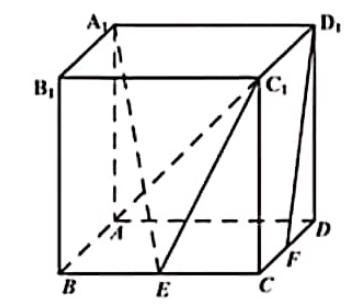
\includegraphics[width=.42\linewidth]{assets/asset-110-01.jpg}
\end{center}
\begin{solution}
\textbf{答案：}（I）证明见解析；（II）$\frac{\sqrt{3}}{9}$；（III）$\frac{1}{3}$

\textbf{分析：}（I）建立空间直角坐标系，求出 $\overrightarrow{D_1F}$ 及平面 $A_1EC_1$ 的一个法向量 $\vec{m}$，证明 $\overrightarrow{D_1F} \perp \vec{m}$，即可得证；
（II）求出 $\overrightarrow{AC_1}$，由 $\sin\theta = |\cos\langle\vec{m},\overrightarrow{AC_1}\rangle|$ 运算即可得解；
（III）求得平面 $AA_1C_1$ 的一个法向量 $\overrightarrow{DB}$，由 $\cos\langle\overrightarrow{DB},\vec{m}\rangle = \frac{\overrightarrow{DB}\cdot\vec{m}}{|\overrightarrow{DB}||\vec{m}|}$ 结合同角三角函数的平方关系即可得解.

\textbf{详解：}（I）以 $A$ 为原点，$AB, AD, AA_1$ 分别为 $x, y, z$ 轴建立空间直角坐标系，则 $A(0,0,0)$，$A_1(0,0,2)$，$B(2,0,0)$，$C(2,2,0)$，$D(0,2,0)$，$C_1(2,2,2)$，$D_1(0,2,2)$，$E(2,1,0)$，$F(1,2,0)$，$\overrightarrow{D_1F} = (1,0,-2)$，$\overrightarrow{A_1C_1} = (2,2,0)$，$\overrightarrow{A_1E} = (2,1,-2)$，设平面 $A_1EC_1$ 的法向量 $\vec{m} = (x_1,y_1,z_1)$，则 $\begin{cases} \vec{m}\cdot\overrightarrow{A_1C_1}=2x_1+2y_1=0 \\ \vec{m}\cdot\overrightarrow{A_1E}=2x_1+y_1-2z_1=0 \end{cases}$，取 $x_1=2$，得 $\vec{m}=(2,-2,1)$，$\because \overrightarrow{D_1F}\cdot\vec{m}=2-2=0$，$\therefore \overrightarrow{D_1F} \perp \vec{m}$，又 $D_1F \not\subset$ 平面 $A_1EC_1$，$\therefore D_1F //$ 平面 $A_1EC_1$；
（II）$\overrightarrow{AC_1} = (2,2,2)$，设直线 $AC_1$ 与平面 $A_1EC_1$ 所成角为 $\theta$，则 $\sin\theta = |\cos\langle\vec{m},\overrightarrow{AC_1}\rangle| = \frac{|\vec{m}\cdot\overrightarrow{AC_1}|}{|\vec{m}||\overrightarrow{AC_1}|} = \frac{|2\times2+(-2)\times2+1\times2|}{\sqrt{2^2+(-2)^2+1^2}\sqrt{2^2+2^2+2^2}} = \frac{2}{3\times 2\sqrt{3}} = \frac{\sqrt{3}}{9}$；
（III）平面 $AA_1C_1$ 的一个法向量为 $\overrightarrow{DB} = (2,-2,0)$，$\cos\langle\overrightarrow{DB},\vec{m}\rangle = \frac{\overrightarrow{DB}\cdot\vec{m}}{|\overrightarrow{DB}||\vec{m}|} = \frac{2\times2+(-2)\times(-2)+0\times1}{\sqrt{4+4}\sqrt{4+4+1}} = \frac{8}{2\sqrt{2}\times3} = \frac{2\sqrt{2}}{3}$，则二面角 $A-A_1C_1-E$ 的正弦值为 $\sqrt{1-\left(\frac{2\sqrt{2}}{3}\right)^2} = \frac{1}{3}$.
\end{solution}
\end{question}

\begin{question}[points=5]
\textbf{来源：}2021 年 新高考II卷，第 4 题\par
北斗三号全球卫星导航系统是我国航天事业的重要成果．在卫星导航系统中，地球静止同步卫星的轨道位于地球赤道所在平面，轨道高度为$36000\text{km}$（轨道高度是指卫星到地球表面的距离）．将地球看作是一个球心为$O$，半径$r$为$6400\text{km}$的球，其上点$A$的纬度是指$OA$与赤道平面所成角的度数．地球表面上能直接观测到一颗地球静止同步轨道卫星点的纬度最大值为$\alpha$，记卫星信号覆盖地球表面的表面积为$S=2\pi r^2(1-\cos\alpha)$（单位：$\text{km}^2$），则$S$占地球表面积的百分比约为（ ）
\begin{choices}
  \item A. $26\%$
  \item B. $34\%$
  \item C. $42\%$
  \item D. $50\%$
\end{choices}
\begin{solution}
\textbf{答案：}C

\textbf{分析：}由题意结合所给的表面积公式和球的表面积公式整理计算即可求得最终结果.

\textbf{详解：}由题意可得，$S$占地球表面积的百分比约为：$\frac{2\pi r^2(1-\cos\alpha)}{4\pi r^2}=\frac{1-\cos\alpha}{2}=\frac{1-\frac{6400}{6400+36000}}{2}\approx0.42=42\%$.故选：C.
\end{solution}
\end{question}

\begin{question}[points=5]
\textbf{来源：}2021 年 新高考II卷，第 5 题\par
正四棱台的上､下底面的边长分别为$2$，$4$，侧棱长为$2$，则其体积为（ ）
\begin{choices}
  \item A. $20+12\sqrt{3}$
  \item B. $28\sqrt{2}$
  \item C. $\frac{56}{3}$
  \item D. $\frac{28\sqrt{2}}{3}$
\end{choices}
\begin{solution}
\textbf{答案：}D

\textbf{分析：}由四棱台的几何特征算出该几何体的高及上下底面面积，再由棱台的体积公式即可得解.

\textbf{详解：}连接该正四棱台上下底面的中心，因为该四棱台上下底面边长分别为2，4，侧棱长为2，所以该棱台的高$h=\sqrt{2^2-(\sqrt{2})^2}=\sqrt{2}$，下底面面积$S_1=16$，上底面面积$S_2=4$，所以该棱台的体积$V=\frac{1}{3}h(S_1+S_2+\sqrt{S_1S_2})=\frac{1}{3}\times\sqrt{2}\times(16+4+\sqrt{64})=\frac{28\sqrt{2}}{3}$.故选：D.
\end{solution}
\end{question}

\begin{question}[points=5]
\textbf{来源：}2021 年 新高考II卷，第 10 题\par
如图，在正方体中，O为底面的中心，P为所在棱的中点，M，N为正方体的顶点．则满足MN⊥OP的是（ ）

\begin{center}
  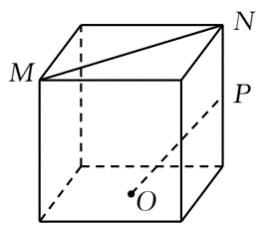
\includegraphics[width=.42\linewidth]{assets/asset-113-01.jpg}
\end{center}
\begin{choices}
  \item A.
  \item B.
  \item C.
  \item D.
\end{choices}
\begin{solution}
\textbf{答案：}BC

\textbf{分析：}根据线面垂直的判定定理可得BC的正误，平移直线MN构造所考虑的线线角后可判断AD的正误.

\textbf{详解：}设正方体棱长为 $2$。对于 A，连接 $AC$，则 $MN\parallel AC$，而在直角三角形 $OPC$ 中，$OC=\sqrt{2}$，$CP=1$，故 $\tan\angle POC=\frac{1}{\sqrt{2}}$，所以 $MN$ 与 $OP$ 不垂直。对于 B，取 $NT$ 的中点 $Q$，连接 $PQ,OQ$，由 $OQ\perp NT$、$OQ\perp SN$ 可得 $OQ\perp$ 平面 $SNTM$，从而 $OQ\perp MN$；又 $PQ\perp MN$，故 $MN\perp$ 平面 $OPQ$，所以 $MN\perp OP$。对于 C，连接 $BD$，则 $BD\parallel MN$，由 B 中的结论知 $OP\perp BD$，所以 $OP\perp MN$。对于 D，平移 $MN$ 后考查相应异面直线所成角，由长度关系可知该角不是直角。因此正确选项为 BC。
\end{solution}
\end{question}

\begin{question}[points=12]
\textbf{来源：}2021 年 新高考II卷，第 19 题\par
在四棱锥$Q-ABCD$中，底面$ABCD$是正方形，若$AD=2$, $QD=QA=\sqrt{5}$, $QC=3$．

（1）证明：平面$QAD\perp$平面$ABCD$；

（2）求二面角$B-QD-A$的平面角的余弦值．
\begin{solution}
\textbf{答案：}(1) 证明见解析；(2) $\frac{2}{3}$.

\textbf{分析：}(1)取$AD$的中点为$O$，连接$QO,CO$，可证$QO\perp$平面$ABCD$，从而得到面$QAD\perp$面$ABCD$； (2)在平面$ABCD$内，过$O$作$OT\parallel CD$，交$BC$于$T$，则$OT\perp AD$，建如图所示的空间坐标系，求出平面$QAD$、平面$BQD$的法向量后可求二面角的余弦值.

\textbf{详解：}(1)取$AD$的中点为$O$，连接$QO,CO$．因为$QA=QD$，$OA=OD$，则$QO\perp AD$，而$AD=2,QA=\sqrt{5}$，故$QO=\sqrt{5-1}=2$．在正方形$ABCD$中，因为$AD=2$，故$DO=1$，故$CO=\sqrt{5}$，因为$QC=3$，故$QC^2=QO^2+OC^2$，故$\triangle QOC$为直角三角形且$QO\perp OC$，因为$OC\cap AD=O$，故$QO\perp$平面$ABCD$，因为$QO\subset$平面$QAD$，故平面$QAD\perp$平面$ABCD$． (2)在平面$ABCD$内，过$O$作$OT\parallel CD$，交$BC$于$T$，则$OT\perp AD$，结合(1)中的$QO\perp$平面$ABCD$，故可建如图所示的空间坐标系．则$D(0,1,0),Q(0,0,2),B(2,-1,0)$，故$\overrightarrow{BQ}=(-2,1,2),\overrightarrow{BD}=(-2,2,0)$．设平面$QBD$的法向量$\vec{n}=(x,y,z)$，则$\begin{cases} \vec{n}\cdot\overrightarrow{BQ}=0 \\ \vec{n}\cdot\overrightarrow{BD}=0 \end{cases}$即$\begin{cases} -2x+y+2z=0 \\ -2x+2y=0 \end{cases}$，取$x=1$，则$y=1,z=\frac{1}{2}$，故$\vec{n}=(1,1,\frac{1}{2})$．而平面$QAD$的法向量为$\vec{m}=(1,0,0)$，故$\cos<\vec{m},\vec{n}>=\frac{1}{1\times\frac{3}{2}}=\frac{2}{3}$．二面角$B-QD-A$的平面角为锐角，故其余弦值为$\frac{2}{3}$.
\end{solution}
\end{question}

\begin{question}[points=5]
\textbf{来源：}2021 年 新高考I卷，第 3 题\par
已知圆锥的底面半径为 $\sqrt{2}$, 其侧面展开图为一个半圆, 则该圆锥的母线长为 ( )
\begin{choices}
  \item $2$
  \item $2\sqrt{2}$
  \item $4$
  \item $4\sqrt{2}$
\end{choices}
\begin{solution}
\textbf{答案：}$2\sqrt{2}$

\textbf{分析：}设圆锥的母线长为 $l$, 根据圆锥底面圆的周长等于扇形的弧长可求得 $l$ 的值.

\textbf{详解：}设圆锥的母线长为 $l$, 由于圆锥底面圆的周长等于扇形的弧长, 则 $\pi l = 2\pi \times \sqrt{2}$, 解得 $l = 2\sqrt{2}$, 故选B.
\end{solution}
\end{question}

\begin{question}[points=5]
\textbf{来源：}2021 年 新高考I卷，第 12 题\par
在正三棱柱 $ABC-A_1B_1C_1$ 中, $AB = AA_1 = 1$, 点 $P$ 满足 $\overrightarrow{BP} = \lambda \overrightarrow{BC} + \mu \overrightarrow{BB_1}$, 其中 $\lambda \in [0,1]$, $\mu \in [0,1]$, 则 ( )
\begin{choices}
  \item 当 $\lambda = 1$ 时, $\triangle AB_1P$ 的周长为定值
  \item 当 $\mu = 1$ 时, 三棱锥 $P-A_1BC$ 的体积为定值
  \item 当 $\lambda = \frac{1}{2}$ 时, 有且仅有一个点 $P$, 使得 $A_1P \perp BP$
  \item 当 $\mu = \frac{1}{2}$ 时, 有且仅有一个点 $P$, 使得 $A_1B \perp$ 平面 $AB_1P$
\end{choices}
\begin{solution}
\textbf{答案：}B, D

\textbf{分析：}将向量关系转化为点的轨迹, 通过建系或几何性质判断.

\textbf{详解：}A: $\lambda = 1$ 时 $P$ 在 $CC_1$ 上, $\triangle AB_1P$ 周长不是定值, 错误; B: $\mu = 1$ 时 $P$ 在 $B_1C_1$ 上, $BC \parallel B_1C_1$, 故 $P$ 到平面 $A_1BC$ 距离为定值, 体积为定值, 正确; C: $\lambda = \frac{1}{2}$ 时 $P$ 在 $BC$ 中点与 $B_1C_1$ 中点的连线上, 建系得 $A_1P \perp BP$ 有 $\mu=0$ 或 $1$, 两个点, 错误; D: $\mu = \frac{1}{2}$ 时 $P$ 在 $BB_1$ 中点与 $CC_1$ 中点的连线上, 建系得 $A_1B \perp$ 平面 $AB_1P$ 时 $P$ 与 $C_1$ 重合, 唯一, 正确. 故选BD.
\end{solution}
\end{question}

\begin{question}[points=12]
\textbf{来源：}2021 年 新高考I卷，第 20 题\par
如图, 在三棱锥 $A-BCD$ 中, 平面 $ABD \perp$ 平面 $BCD$, $AB = AD$, $O$ 为 $BD$ 的中点.

(1) 证明: $OA \perp CD$;

(2) 若 $\triangle OCD$ 是边长为1的等边三角形, 点 $E$ 在棱 $AD$ 上, $DE = 2EA$, 且二面角 $E-BC-D$ 的大小为 $45^\circ$, 求三棱锥 $A-BCD$ 的体积.

\begin{center}
  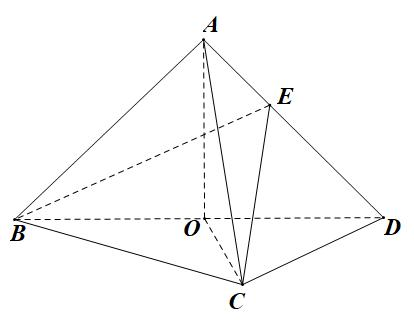
\includegraphics[width=.42\linewidth]{assets/asset-117-01.jpg}
\end{center}
\begin{solution}
\textbf{答案：}(1) 证明见解析; (2) $\frac{\sqrt{3}}{6}$

\textbf{分析：}(1) 利用面面垂直性质定理得 $AO \perp$ 平面 $BCD$, 从而 $AO \perp CD$. (2) 作出二面角平面角, 求得高, 再求体积.

\textbf{详解：}(1) 因为 $AB = AD$, $O$ 为 $BD$ 中点, 所以 $AO \perp BD$. 又平面 $ABD \perp$ 平面 $BCD$, 交线为 $BD$, $AO \subset$ 平面 $ABD$, 所以 $AO \perp$ 平面 $BCD$. 因为 $CD \subset$ 平面 $BCD$, 所以 $AO \perp CD$.
(2) 作 $EF \perp BD$ 于 $F$, 作 $FM \perp BC$ 于 $M$, 连接 $EM$. 由(1)知 $AO \perp$ 平面 $BCD$, 故 $EF \perp$ 平面 $BCD$, 则 $EF \perp BC$. 又 $FM \perp BC$, 所以 $BC \perp$ 平面 $EFM$, 故 $\angle EMF$ 为二面角 $E-BC-D$ 的平面角, $\angle EMF = 45^\circ$. 由 $\triangle OCD$ 为正三角形, $O$ 为 $BD$ 中点, 可得 $BD = 2$, $BC = \sqrt{3}$. 由 $DE = 2EA$ 得 $DF = \frac{2}{3}DO = \frac{2}{3}$, $BF = \frac{4}{3}$. $FM = \frac{1}{2}BF = \frac{2}{3}$, 在等腰直角三角形 $EFM$ 中, $EF = FM = \frac{2}{3}$, 故 $AO = \frac{2}{3} \times \frac{3}{2} = 1$? 实际上 $AO = 1$ (由相似或比例得到). 所以 $V_{A-BCD} = \frac{1}{3} \times AO \times S_{\triangle BCD} = \frac{1}{3} \times 1 \times \frac{1}{2} \times 2 \times \sqrt{3} = \frac{\sqrt{3}}{6}$.
\end{solution}
\end{question}

\begin{question}[points=4]
\textbf{来源：}2021 年 浙江卷，第 4 题\par
某几何体的三视图如图所示，则该几何体的体积是（   ）
\begin{choices}
  \item $\frac{3}{2}$
  \item $3$
  \item $\frac{3\sqrt{2}}{2}$
  \item $3\sqrt{2}$
\end{choices}
\begin{solution}
\textbf{答案：}A

\textbf{分析：}根据三视图可得几何体为四棱柱, 根据棱柱的体积公式可求其体积.

\textbf{详解：}几何体为四棱柱, 高为1, 底面为等腰梯形, 上底为 $\sqrt{2}$, 下底为 $2\sqrt{2}$, 腰长为1, 故梯形的高为 $\sqrt{1^2 - \left(\frac{\sqrt{2}}{2}\right)^2} = \frac{\sqrt{2}}{2}$, 体积 $V = \frac{1}{2}(\sqrt{2}+2\sqrt{2})\times\frac{\sqrt{2}}{2}\times1 = \frac{3}{2}$.
\end{solution}
\end{question}

\begin{question}[points=4]
\textbf{来源：}2021 年 浙江卷，第 6 题\par
如图已知正方体 $ABCD-A_1B_1C_1D_1$, $M,N$ 分别是 $A_1D$, $D_1B$ 的中点, 则（   ）
\begin{choices}
  \item 直线 $A_1D$ 与直线 $D_1B$ 垂直, 直线 $MN //$ 平面 $ABCD$
  \item 直线 $A_1D$ 与直线 $D_1B$ 平行, 直线 $MN \perp$ 平面 $BDD_1B_1$
  \item 直线 $A_1D$ 与直线 $D_1B$ 相交, 直线 $MN //$ 平面 $ABCD$
  \item 直线 $A_1D$ 与直线 $D_1B$ 异面, 直线 $MN \perp$ 平面 $BDD_1B_1$
\end{choices}
\begin{solution}
\textbf{答案：}A

\textbf{分析：}由正方体间的垂直、平行关系, 可证 $MN // AB$, $A_1D \perp$ 平面 $ABD_1$, 即可得出结论.

\textbf{详解：}连 $AD_1$, $M$ 是 $A_1D$ 中点, 所以 $M$ 为 $AD_1$ 中点, 又 $N$ 是 $D_1B$ 中点, 所以 $MN // AB$, 故 $MN //$ 平面 $ABCD$; 由正方体性质, $A_1D \perp AD_1$, $AB \perp A_1D$, 所以 $A_1D \perp$ 平面 $ABD_1$, 从而 $A_1D \perp D_1B$, 且异面.
\end{solution}
\end{question}

\begin{question}[points=15]
\textbf{来源：}2021 年 浙江卷，第 19 题\par
如图，在四棱锥 $P-ABCD$ 中，底面 $ABCD$ 是平行四边形，$\angle ABC=120^\circ$, $AB=1$, $BC=4$, $PA=\sqrt{15}$, $M,N$ 分别为 $BC, PC$ 的中点，$PD\perp DC$, $PM\perp MD$.

(1) 证明：$AB\perp PM$；

(2) 求直线 $AN$ 与平面 $PDM$ 所成角的正弦值.
\begin{solution}
\textbf{答案：}(1) 见解析; (2) $\frac{\sqrt{15}}{6}$

\textbf{分析：}(1) 先证 $DC\perp$ 平面 $PDM$, 再由 $AB\parallel DC$ 得 $AB\perp PM$; (2) 建立空间直角坐标系, 利用向量法求线面角.

\textbf{详解：}(1) 在 $\triangle DCM$ 中, $DC=1,CM=2,\angle DCM=60^\circ$, 由余弦定理得 $DM=\sqrt{3}$. 由 $DM^2+DC^2=CM^2$ 得 $DM\perp DC$. 又 $PD\perp DC$, $PD\cap DM=D$, 故 $DC\perp$ 平面 $PDM$, 从而 $DC\perp PM$. 又 $AB\parallel DC$, 所以 $AB\perp PM$.
(2) 由 $PM\perp MD$ 及 (1) 得 $PM\perp$ 平面 $ABCD$. 以 $M$ 为原点, $MD$ 为 $x$ 轴, $ME$ ( $E$ 为 $AD$ 中点) 为 $y$ 轴, $MP$ 为 $z$ 轴建立空间直角坐标系. 则 $A(-\sqrt{3},2,0)$, $D(\sqrt{3},0,0)$, $P(0,0,2\sqrt{2})$, $C(\sqrt{3},-1,0)$, $N(\frac{\sqrt{3}}{2},-\frac12,\sqrt{2})$, 所以 $\overrightarrow{AN}=(\frac{3\sqrt{3}}{2},-\frac52,\sqrt{2})$. 平面 $PDM$ 的法向量为 $\vec{n}=(0,1,0)$. 则 $\sin\theta = \frac{|\overrightarrow{AN}\cdot\vec{n}|}{|\overrightarrow{AN}|\cdot|\vec{n}|} = \frac{5/2}{\sqrt{\frac{27}{4}+\frac{25}{4}+2}} = \frac{5/2}{\sqrt{15}} = \frac{\sqrt{15}}{6}$.
\end{solution}
\end{question}

\section*{2022 年}

\begin{question}[points=4]
\textbf{来源：}2022 年 北京卷，第 9 题\par
已知正三棱锥 $P-ABC$ 的六条棱长均为6，$S$ 是 $\triangle ABC$ 及其内部的点构成的集合。设集合 $T = \{ Q \in S \mid PQ \leq 5 \}$，则 $T$ 表示的区域的面积为
\begin{choices}
  \item $\dfrac{3\pi}{4}$
  \item $\pi$
  \item $2\pi$
  \item $3\pi$
\end{choices}
\begin{solution}
\textbf{答案：}B

\textbf{分析：}求出以 $P$ 为球心，5为半径的球与底面 $ABC$ 的截面圆的半径后可求区域的面积。

\textbf{详解：}设顶点 $P$ 在底面上的投影为 $O$，连接 $BO$，则 $O$ 为三角形 $ABC$ 的中心，且 $BO = \dfrac{2}{3} \times 6 \times \dfrac{\sqrt{3}}{2} = 2\sqrt{3}$，故 $PO = \sqrt{36 - 12} = 2\sqrt{6}$。因为 $PQ = 5$，故 $OQ = 1$。故 $T$ 的轨迹为以 $O$ 为圆心，1为半径的圆。三角形 $ABC$ 内切圆的圆心为 $O$，半径为 $\dfrac{2 \times \frac{\sqrt{3}}{4} \times 36}{3 \times 6} = \sqrt{3} > 1$，故该圆在三角形 $ABC$ 内部，其面积为 $\pi$。故选B。
\end{solution}
\end{question}

\begin{question}[points=14]
\textbf{来源：}2022 年 北京卷，第 17 题\par
如图，在三棱柱 $ABC-A_1B_1C_1$ 中，侧面 $BCC_1B_1$ 为正方形，平面 $BCC_1B_1 \perp$ 平面 $ABB_1A_1$，$AB=BC=2$，$M,N$ 分别为 $A_1B_1$，$AC$ 的中点。

（1）求证：$MN \parallel$ 平面 $BCC_1B_1$；

（2）再从条件①、条件②这两个条件中选择一个作为已知，求直线 $AB$ 与平面 $BMN$ 所成角的正弦值。

条件①：$AB \perp MN$；

条件②：$BM = MN$。

注：如果选择条件①和条件②分别解答，按第一个解答计分。

\begin{center}
  
\includegraphics[width=.42\linewidth]{assets/asset-122-01.jpg}
\end{center}
\begin{solution}
\textbf{答案：}（1）见解析；（2）$\dfrac{2}{3}$

\textbf{分析：}（1）取 $AB$ 的中点为 $K$，连接 $MK,NK$，可证平面 $MKN\parallel$ 平面 $CBB_1C_1$，从而可证 $MN\parallel$ 平面 $CBB_1C_1$。
（2）选①②均可证明 $BB_1\perp$ 平面 $ABC$，从而可建立空间直角坐标系，利用空间向量可求线面角的正弦值。

\textbf{详解：}（1）证明：取 $AB$ 的中点为 $K$，连接 $MK,NK$。由三棱柱 $ABC-A_1B_1C_1$ 可得四边形 $ABB_1A_1$ 为平行四边形，而 $B_1M=MA_1$，$BK=KA$，则 $MK\parallel BB_1$，而 $MK\not\subset$ 平面 $CBB_1C_1$，$BB_1\subset$ 平面 $CBB_1C_1$，故 $MK\parallel$ 平面 $CBB_1C_1$。而 $CN=NA$，$BK=KA$，则 $NK\parallel BC$，同理可得 $NK\parallel$ 平面 $CBB_1C_1$。而 $NK\cap MK=K$，$NK,MK\subset$ 平面 $MKN$，故平面 $MKN\parallel$ 平面 $CBB_1C_1$，而 $MN\subset$ 平面 $MKN$，故 $MN\parallel$ 平面 $CBB_1C_1$。
（2）解：因为侧面 $CBB_1C_1$ 为正方形，故 $CB\perp BB_1$，而 $CB\subset$ 平面 $CBB_1C_1$，平面 $CBB_1C_1\perp$ 平面 $ABB_1A_1$，平面 $CBB_1C_1\cap$ 平面 $ABB_1A_1 = BB_1$，故 $CB\perp$ 平面 $ABB_1A_1$。因为 $NK\parallel BC$，故 $NK\perp$ 平面 $ABB_1A_1$。因为 $AB\subset$ 平面 $ABB_1A_1$，故 $NK\perp AB$。
若选①，则 $AB\perp MN$，而 $NK\perp AB$，$NK\cap MN=N$，故 $AB\perp$ 平面 $MNK$，而 $MK\subset$ 平面 $MNK$，故 $AB\perp MK$，所以 $AB\perp BB_1$。而 $CB\perp BB_1$，$CB\cap AB=B$，故 $BB_1\perp$ 平面 $ABC$。
若选②，因为 $NK\parallel BC$，故 $NK\perp$ 平面 $ABB_1A_1$，而 $KM\subset$ 平面 $MKN$，故 $NK\perp KM$，又 $B_1M=BK=1$，$NK=1$，故 $B_1M=NK$，而 $B_1B=MK=2$，$MB=MN$，故 $\triangle BB_1M\cong \triangle MKN$，所以 $\angle BB_1M = \angle MKN = 90^\circ$，故 $A_1B_1\perp BB_1$。而 $CB\perp BB_1$，$CB\cap AB=B$，故 $BB_1\perp$ 平面 $ABC$。
建立空间直角坐标系，则 $B(0,0,0)$，$A(0,2,0)$，$N(1,1,0)$，$M(0,1,2)$。$\overrightarrow{BA}=(0,2,0)$，$\overrightarrow{BN}=(1,1,0)$，$\overrightarrow{BM}=(0,1,2)$。设平面 $BNM$ 的法向量为 $\vec{n}=(x,y,z)$，则 $\begin{cases} \vec{n}\cdot\overrightarrow{BN}=0 \\ \vec{n}\cdot\overrightarrow{BM}=0 \end{cases}$，即 $\begin{cases} x+y=0 \\ y+2z=0 \end{cases}$，取 $z=-1$，则 $\vec{n}=(-2,2,-1)$。设直线 $AB$ 与平面 $BNM$ 所成的角为 $\theta$，则 $\sin\theta = |\cos\langle\vec{n},\overrightarrow{BA}\rangle| = \dfrac{|\vec{n}\cdot\overrightarrow{BA}|}{|\vec{n}||\overrightarrow{BA}|} = \dfrac{4}{2\times 3} = \dfrac{2}{3}$。
\end{solution}
\end{question}

\begin{question}[points=5]
\textbf{来源：}2022 年 全国甲卷-理科，第 4 题\par
如图，网格纸上绘制的是一个多面体的三视图，网格小正方形的边长为1，则该多面体的体积为（ ）

\begin{center}
  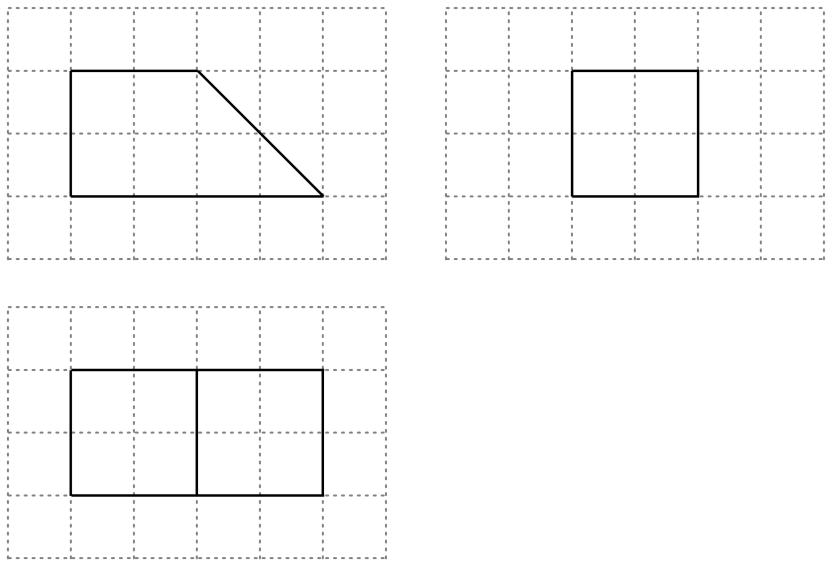
\includegraphics[width=.42\linewidth]{assets/asset-123-01.jpg}
\end{center}
\begin{choices}
  \item $8$
  \item $12$
  \item $16$
  \item $20$
\end{choices}
\begin{solution}
\textbf{答案：}B

\textbf{分析：}由三视图还原几何体，再由棱柱的体积公式即可得解.

\textbf{详解：}由三视图还原几何体如图，则该直四棱柱的体积 $V = \frac{2+4}{2} \times 2 \times 2 = 12$. 故选B.
\end{solution}
\end{question}

\begin{question}[points=5]
\textbf{来源：}2022 年 全国甲卷-理科，第 7 题\par
在长方体 $ABCD-A_1B_1C_1D_1$ 中，已知 $B_1D$ 与平面 $ABCD$ 和平面 $AA_1B_1B$ 所成的角均为 $30^\circ$，则（ ）
\begin{choices}
  \item $AB=2AD$
  \item $AB$ 与平面 $AB_1C_1D$ 所成的角为 $30^\circ$
  \item $AC=CB_1$
  \item $B_1D$ 与平面 $BB_1C_1C$ 所成的角为 $45^\circ$
\end{choices}
\begin{solution}
\textbf{答案：}D

\textbf{分析：}根据线面角的定义以及长方体的结构特征即可求出.

\textbf{详解：}不妨设 $AB=a$, $AD=b$, $AA_1=c$，依题以及长方体的结构特征可知，$B_1D$ 与平面 $ABCD$ 所成角为 $\angle B_1DB$，$B_1D$ 与平面 $AA_1B_1B$ 所成角为 $\angle DB_1A$，所以 $\sin30^\circ=\frac{c}{B_1D}=\frac{b}{B_1D}$，即 $b=c$, $B_1D=2c=\sqrt{a^2+b^2+c^2}$，解得 $a=\sqrt{2}c$. 对于A，$AB=a$, $AD=b$, $AB=\sqrt{2}AD$，A错误；对于B，过B作 $BE\perp AB_1$ 于E，易知 $BE\perp$ 平面 $AB_1C_1D$，所以AB与平面 $AB_1C_1D$ 所成角为 $\angle BAE$，因为 $\tan\angle BAE=\frac{c}{a}=\frac{\sqrt{2}}{2}$，所以 $\angle BAE\neq30^\circ$，B错误；对于C，$AC=\sqrt{a^2+b^2}=\sqrt{3}c$, $CB_1=\sqrt{b^2+c^2}=\sqrt{2}c$，$AC\neq CB_1$，C错误；对于D，$B_1D$ 与平面 $BB_1C_1C$ 所成角为 $\angle DB_1C$，$\sin\angle DB_1C=\frac{CD}{B_1D}=\frac{a}{2c}=\frac{\sqrt{2}}{2}$，而 $0<\angle DB_1C<90^\circ$，所以 $\angle DB_1C=45^\circ$，D正确. 故选D.
\end{solution}
\end{question}

\begin{question}[points=5]
\textbf{来源：}2022 年 全国甲卷-理科，第 9 题\par
甲、乙两个圆锥的母线长相等，侧面展开图的圆心角之和为 $2\pi$，侧面积分别为 $S_\text{甲}$ 和 $S_\text{乙}$，体积分别为 $V_\text{甲}$ 和 $V_\text{乙}$. 若 $\frac{S_\text{甲}}{S_\text{乙}}=2$，则 $\frac{V_\text{甲}}{V_\text{乙}}=$（ ）
\begin{choices}
  \item $\sqrt{5}$
  \item $2\sqrt{2}$
  \item $\sqrt{10}$
  \item $\frac{5\sqrt{10}}{4}$
\end{choices}
\begin{solution}
\textbf{答案：}C

\textbf{分析：}设母线长为l，甲圆锥底面半径为$r_1$，乙圆锥底面圆半径为$r_2$，根据圆锥的侧面积公式可得$r_1=2r_2$，再结合圆心角之和可将$r_1,r_2$分别用l表示，再利用勾股定理分别求出两圆锥的高，再根据圆锥的体积公式即可得解.

\textbf{详解：}设母线长为l，甲圆锥底面半径为$r_1$，乙圆锥底面圆半径为$r_2$，则 $\frac{S_\text{甲}}{S_\text{乙}}=\frac{\pi r_1 l}{\pi r_2 l}=\frac{r_1}{r_2}=2$，所以 $r_1=2r_2$，又 $\frac{2\pi r_1}{l}+\frac{2\pi r_2}{l}=2\pi$，则 $\frac{r_1+r_2}{l}=1$，所以 $r_1=\frac{2}{3}l$, $r_2=\frac{1}{3}l$，所以甲圆锥的高 $h_1=\sqrt{l^2-\frac{4}{9}l^2}=\frac{\sqrt{5}}{3}l$，乙圆锥的高 $h_2=\sqrt{l^2-\frac{1}{9}l^2}=\frac{2\sqrt{2}}{3}l$，所以 $\frac{V_\text{甲}}{V_\text{乙}}=\frac{\frac{1}{3}\pi r_1^2 h_1}{\frac{1}{3}\pi r_2^2 h_2}=\frac{\frac{4}{9}l^2 \times \frac{\sqrt{5}}{3}l}{\frac{1}{9}l^2 \times \frac{2\sqrt{2}}{3}l}=\sqrt{10}$. 故选C.
\end{solution}
\end{question}

\begin{question}[points=12]
\textbf{来源：}2022 年 全国甲卷-理科，第 18 题\par
在四棱锥 $P-ABCD$ 中，$PD\perp$ 底面 $ABCD$, $CD\parallel AB$, $AD=DC=CB=1$, $AB=2$, $DP=\sqrt{3}$.

(1) 证明：$BD\perp PA$;

(2) 求 $PD$ 与平面 $PAB$ 所成的角的正弦值.

\begin{center}
  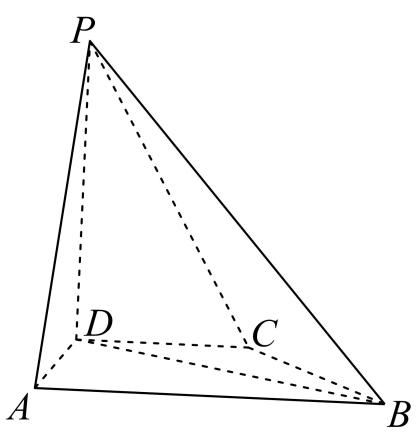
\includegraphics[width=.42\linewidth]{assets/asset-126-01.jpg}
\end{center}
\begin{solution}
\textbf{答案：}(1) 证明见解析；(2) $\frac{\sqrt{5}}{5}$

\textbf{分析：}(1) 作 $DE\perp AB$ 于E，$CF\perp AB$ 于F，利用勾股定理证明 $AD\perp BD$，根据线面垂直的性质可得 $PD\perp BD$，从而可得 $BD\perp$ 平面 $PAD$，再根据线面垂直的性质即可得证. (2) 以点D为原点建立空间直角坐标系，利用向量法即可得出答案.

\textbf{详解：}(1) 在四边形 $ABCD$ 中，作 $DE\perp AB$ 于E，$CF\perp AB$ 于F，因为 $CD\parallel AB$, $AD=CD=CB=1$, $AB=2$，所以四边形 $ABCD$ 为等腰梯形，所以 $AE=BF=\frac{1}{2}$，故 $DE=\frac{\sqrt{3}}{2}$, $BD=\sqrt{DE^2+BE^2}=\sqrt{3}$，所以 $AD^2+BD^2=AB^2$，所以 $AD\perp BD$. 因为 $PD\perp$ 平面 $ABCD$, $BD\subset$ 平面 $ABCD$，所以 $PD\perp BD$，又 $PD\cap AD=D$，所以 $BD\perp$ 平面 $PAD$，又因为 $PA\subset$ 平面 $PAD$，所以 $BD\perp PA$.
(2) 以点D为原点建立空间直角坐标系，$BD=\sqrt{3}$，则 $A(1,0,0)$, $B(0,\sqrt{3},0)$, $P(0,0,\sqrt{3})$，则 $\overrightarrow{AP}=(-1,0,\sqrt{3})$, $\overrightarrow{BP}=(0,-\sqrt{3},\sqrt{3})$, $\overrightarrow{DP}=(0,0,\sqrt{3})$，设平面 $PAB$ 的法向量 $\vec{n}=(x,y,z)$，则有 $\begin{cases} \vec{n}\cdot\overrightarrow{AP}=-x+\sqrt{3}z=0 \\ \vec{n}\cdot\overrightarrow{BP}=-\sqrt{3}y+\sqrt{3}z=0 \end{cases}$，可取 $\vec{n}=(\sqrt{3},1,1)$，则 $\cos\langle\vec{n},\overrightarrow{DP}\rangle=\frac{\vec{n}\cdot\overrightarrow{DP}}{|\vec{n}||\overrightarrow{DP}|}=\frac{\sqrt{3}}{\sqrt{5}\times\sqrt{3}}=\frac{\sqrt{5}}{5}$，所以 $PD$ 与平面 $PAB$ 所成角的正弦值为 $\frac{\sqrt{5}}{5}$.
\end{solution}
\end{question}

\begin{question}[points=5]
\textbf{来源：}2022 年 全国甲卷-文科，第 4 题\par
如图，网格纸上绘制的是一个多面体的三视图，网格小正方形的边长为1，则该多面体的体积为
\begin{choices}
  \item A．8
  \item B．12
  \item C．16
  \item D．20
\end{choices}
\begin{solution}
\textbf{答案：}B
\end{solution}
\end{question}

\begin{question}[points=5]
\textbf{来源：}2022 年 全国甲卷-文科，第 9 题\par
在长方体 $ABCD-A_1B_1C_1D_1$ 中，已知 $B_1D$ 与平面 $ABCD$ 和平面 $AA_1B_1B$ 所成的角均为 $30^\circ$，则
\begin{choices}
  \item A．$AB=2AD$
  \item B．$AB$ 与平面 $AB_1C_1D$ 所成的角为 $30^\circ$
  \item C．$AC=CB_1$
  \item D．$B_1D$ 与平面 $BB_1C_1C$ 所成的角为 $45^\circ$
\end{choices}
\begin{solution}
\textbf{答案：}D
\end{solution}
\end{question}

\begin{question}[points=5]
\textbf{来源：}2022 年 全国甲卷-文科，第 10 题\par
甲、乙两个圆锥的母线长相等，侧面展开图的圆心角之和为 $2\pi$，侧面积分别为 $S_{\text{甲}}$ 和 $S_{\text{乙}}$，体积分别为 $V_{\text{甲}}$ 和 $V_{\text{乙}}$．若 $\frac{S_{\text{甲}}}{S_{\text{乙}}}=2$，则 $\frac{V_{\text{甲}}}{V_{\text{乙}}}=$
\begin{choices}
  \item $\sqrt{5}$
  \item $2\sqrt{2}$
  \item $\sqrt{10}$
  \item $\frac{5\sqrt{10}}{4}$
\end{choices}
\begin{solution}
\textbf{答案：}C
\end{solution}
\end{question}

\begin{question}[points=12]
\textbf{来源：}2022 年 全国甲卷-文科，第 19 题\par
小明同学参加综合实践活动，设计了一个封闭的包装盒，包装盒如图所示：底面 $ABCD$ 是边长为8（单位：cm）的正方形，$\triangle EAB, \triangle FBC, \triangle GCD, \triangle HDA$ 均为正三角形，且它们所在的平面都与平面 $ABCD$ 垂直．

（1）证明：$EF\parallel$ 平面 $ABCD$；

（2）求该包装盒的容积（不计包装盒材料的厚度）．

\begin{center}
  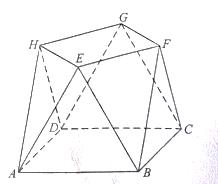
\includegraphics[width=.42\linewidth]{assets/asset-130-01.jpg}
\end{center}
\begin{solution}
\textbf{答案：}（1）证明见解析；（2）$\frac{640}{3}\sqrt{3}$
\end{solution}
\end{question}

\begin{question}[points=5]
\textbf{来源：}2022 年 全国乙卷-理科，第 7 题\par
在正方体$ABCD-A_1B_1C_1D_1$中，$E$，$F$分别为$AB$，$BC$的中点，则（\qquad）
\begin{choices}
  \item 平面$B_1EF \perp$平面$BDD_1$
  \item 平面$B_1EF \perp$平面$A_1BD$
  \item 平面$B_1EF \parallel$平面$A_1AC$
  \item 平面$B_1EF \parallel$平面$A_1C_1D$
\end{choices}
\begin{solution}
\textbf{答案：}A

\textbf{分析：}证明$EF \perp$平面$BDD_1$，即可判断A；如图，以点$D$为原点，建立空间直角坐标系，设$AB=2$，分别求出平面$B_1EF$，$A_1BD$，$A_1C_1D$的法向量，根据法向量的位置关系，即可判断BCD.

\textbf{详解：}解：在正方体$ABCD-A_1B_1C_1D_1$中，\\$AC \perp BD$且$DD_1 \perp$平面$ABCD$，又$EF \subset$平面$ABCD$，所以$EF \perp DD_1$，因为$E,F$分别为$AB,BC$的中点，所以$EF \parallel AC$，所以$EF \perp BD$，又$BD \cap DD_1 = D$，所以$EF \perp$平面$BDD_1$，又$EF \subset$平面$B_1EF$，所以平面$B_1EF \perp$平面$BDD_1$，故A正确；如图，以点$D$为原点，建立空间直角坐标系，设$AB=2$，则$B_1(2,2,2), E(2,1,0), F(1,2,0), B(2,2,0), A_1(2,0,2), A(2,0,0), C(0,2,0), C_1(0,2,2)$，\\$\overrightarrow{EF}=(-1,1,0), \overrightarrow{EB_1}=(0,1,2), \overrightarrow{DB}=(2,2,0), \overrightarrow{DA_1}=(2,0,2), \overrightarrow{AA_1}=(0,0,2), \overrightarrow{AC}=(-2,2,0), \overrightarrow{A_1C_1}=(-2,2,0)$，设平面$B_1EF$的法向量为$\vec{m}=(x_1,y_1,z_1)$，则有$\begin{cases} \vec{m}\cdot\overrightarrow{EF}=-x_1+y_1=0 \\ \vec{m}\cdot\overrightarrow{EB_1}=y_1+2z_1=0 \end{cases}$，可取$\vec{m}=(2,2,-1)$，同理可得平面$A_1BD$的法向量为$\vec{n_1}=(1,-1,-1)$，平面$A_1AC$的法向量为$\vec{n_2}=(1,1,0)$，平面$A_1C_1D$的法向量为$\vec{n_3}=(1,1,-1)$，则$\vec{m}\cdot\vec{n_1}=2-2+1=1\neq0$，所以平面$B_1EF$与平面$A_1BD$不垂直，故B错误；因为$\vec{m}$与$\vec{n_2}$不平行，所以平面$B_1EF$与平面$A_1AC$不平行，故C错误；因为$\vec{m}$与$\vec{n_3}$不平行，所以平面$B_1EF$与平面$A_1C_1D$不平行，故D错误.
\end{solution}
\end{question}

\begin{question}[points=5]
\textbf{来源：}2022 年 全国乙卷-理科，第 9 题\par
已知球$O$的半径为1，四棱锥的顶点为$O$，底面的四个顶点均在球$O$的球面上，则当该四棱锥的体积最大时，其高为（\qquad）
\begin{choices}
  \item $\frac{1}{3}$
  \item $\frac{1}{2}$
  \item $\frac{\sqrt{3}}{3}$
  \item $\frac{\sqrt{2}}{2}$
\end{choices}
\begin{solution}
\textbf{答案：}C

\textbf{分析：}先证明当四棱锥的顶点$O$到底面$ABCD$所在小圆距离一定时，底面$ABCD$面积最大值为$2r^2$，进而得到四棱锥体积表达式，再利用均值定理去求四棱锥体积的最大值，从而得到当该四棱锥的体积最大时其高的值.

\textbf{详解：}设该四棱锥底面为四边形$ABCD$，四边形$ABCD$所在小圆半径为$r$，设四边形$ABCD$对角线夹角为$\alpha$，则$S_{ABCD} = \frac{1}{2}\cdot AC\cdot BD\cdot\sin\alpha \leq \frac{1}{2}\cdot AC\cdot BD \leq \frac{1}{2}\cdot 2r\cdot 2r = 2r^2$（当且仅当四边形$ABCD$为正方形时等号成立）即当四棱锥的顶点$O$到底面$ABCD$所在小圆距离一定时，底面$ABCD$面积最大值为$2r^2$又$r^2 + h^2 = 1$则$V_{O-ABCD} = \frac{1}{3}\cdot 2r^2\cdot h = \frac{2}{3}r\cdot r\cdot 2h^2 \leq \frac{2}{3}\left(\frac{r^2 + r^2 + 2h^2}{3}\right)^3 = \frac{4\sqrt{3}}{27}$当且仅当$r^2 = 2h^2$即$h = \frac{\sqrt{3}}{3}$时等号成立.
\end{solution}
\end{question}

\begin{question}[points=12]
\textbf{来源：}2022 年 全国乙卷-理科，第 18 题\par
如图，四面体$ABCD$中，$AD\perp CD, AD=CD, \angle ADB = \angle BDC$，$E$为$AC$的中点．

(1)证明：平面$BED \perp$平面$ACD$；

(2)设$AB=BD=2, \angle ACB=60^{\circ}$，点$F$在$BD$上，当$\triangle AFC$的面积最小时，求$CF$与平面$ABD$所成的角的正弦值．

\begin{center}
  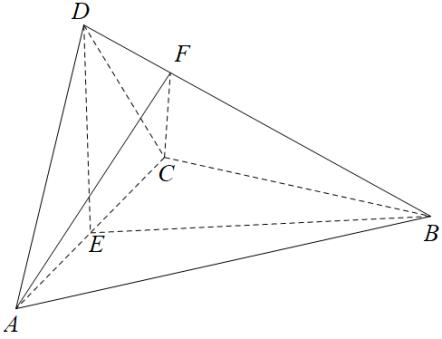
\includegraphics[width=.42\linewidth]{assets/asset-133-01.jpg}
\end{center}
\begin{solution}
\textbf{答案：}(1)证明过程见解析 (2)$\frac{4\sqrt{3}}{7}$

\textbf{分析：}(1)根据已知关系证明$\triangle ABD \cong \triangle CBD$，得到$AB=CB$，结合等腰三角形三线合一得到垂直关系，结合面面垂直的判定定理即可证明；(2)根据勾股定理逆用得到$BE\perp DE$，从而建立空间直角坐标系，结合线面角的运算法则进行计算即可.

\textbf{详解：}【小问1详解】因为$AD=CD$，$E$为$AC$的中点，所以$AC\perp DE$；在$\triangle ABD$和$\triangle CBD$中，因为$AD=CD, \angle ADB=\angle CDB, DB=DB$，所以$\triangle ABD \cong \triangle CBD$，所以$AB=CB$，又因为$E$为$AC$的中点，所以$AC\perp BE$；又因为$DE, BE\subset$平面$BED$，$DE\cap BE=E$，所以$AC\perp$平面$BED$，因为$AC\subset$平面$ACD$，所以平面$BED\perp$平面$ACD$.\\【小问2详解】连接$EF$，由(1)知，$AC\perp$平面$BED$，因为$EF\subset$平面$BED$，所以$AC\perp EF$，所以$S_{\triangle AFC}=\frac{1}{2}AC\cdot EF$，当$EF\perp BD$时，$EF$最小，即$\triangle AFC$的面积最小.因为$\triangle ABD\cong\triangle CBD$，所以$CB=AB=2$，又因为$\angle ACB=60^{\circ}$，所以$\triangle ABC$是等边三角形，因为$E$为$AC$的中点，所以$AE=EC=1$，$BE=\sqrt{3}$，因为$AD\perp CD$，所以$DE=\frac{1}{2}AC=1$，在$\triangle DEB$中，$DE^2+BE^2=BD^2$，所以$BE\perp DE$.以$E$为坐标原点建立如图所示的空间直角坐标系$E-xyz$，则$A(1,0,0), B(0,\sqrt{3},0), D(0,0,1)$，所以$\overrightarrow{AD}=(-1,0,1), \overrightarrow{AB}=(-1,\sqrt{3},0)$，设平面$ABD$的一个法向量为$\vec{n}=(x,y,z)$，则$\begin{cases} \vec{n}\cdot\overrightarrow{AD} = -x+z=0 \\ \vec{n}\cdot\overrightarrow{AB} = -x+\sqrt{3}y=0 \end{cases}$，取$y=\sqrt{3}$，则$\vec{n}=(3,\sqrt{3},3)$，又因为$C(-1,0,0), F\left(0,\frac{\sqrt{3}}{4},\frac{3}{4}\right)$，所以$\overrightarrow{CF}=\left(1,\frac{\sqrt{3}}{4},\frac{3}{4}\right)$，所以$\cos\langle\vec{n},\overrightarrow{CF}\rangle = \frac{\vec{n}\cdot\overrightarrow{CF}}{|\vec{n}||\overrightarrow{CF}|} = \frac{6}{\sqrt{21}\times\frac{7}{4}} = \frac{4\sqrt{3}}{7}$，设$CF$与平面$ABD$所成的角的正弦值为$\theta\left(0\leq\theta\leq\frac{\pi}{2}\right)$，所以$\sin\theta = |\cos\langle\vec{n},\overrightarrow{CF}\rangle| = \frac{4\sqrt{3}}{7}$，所以$CF$与平面$ABD$所成的角的正弦值为$\frac{4\sqrt{3}}{7}$.
\end{solution}
\end{question}

\begin{question}[points=5]
\textbf{来源：}2022 年 全国乙卷-文科，第 9 题\par
在正方体 $ABCD-A_1B_1C_1D_1$ 中，$E,F$ 分别为 $AB, BC$ 的中点，则
\begin{choices}
  \item 平面 $B_1EF \perp$ 平面 $BDD_1$
  \item 平面 $B_1EF \perp$ 平面 $A_1BD$
  \item 平面 $B_1EF \parallel$ 平面 $A_1AC$
  \item 平面 $B_1EF \parallel$ 平面 $A_1C_1D$
\end{choices}
\begin{solution}
\textbf{答案：}A

\textbf{分析：}证明 $EF \perp$ 平面 $BDD_1$, 即可判断A；如图建系，分别求出法向量判断BCD.

\textbf{详解：}在正方体中，$EF \parallel AC$, $AC \perp BD$, 且 $DD_1 \perp$ 底面 $ABCD$, 所以 $EF \perp BD$, $EF \perp DD_1$, 故 $EF \perp$ 平面 $BDD_1$, 又 $EF \subset$ 平面 $B_1EF$, 所以平面 $B_1EF \perp$ 平面 $BDD_1$, A正确. 建系可验证其余错误.
\end{solution}
\end{question}

\begin{question}[points=5]
\textbf{来源：}2022 年 全国乙卷-文科，第 12 题\par
已知球 $O$ 的半径为1，四棱锥的顶点为 $O$, 底面的四个顶点均在球 $O$ 的球面上，则当该四棱锥的体积最大时，其高为
\begin{choices}
  \item $\frac{1}{3}$
  \item $\frac{1}{2}$
  \item $\frac{\sqrt{3}}{3}$
  \item $\frac{\sqrt{2}}{2}$
\end{choices}
\begin{solution}
\textbf{答案：}C

\textbf{分析：}证明当四棱锥为正四棱锥时体积最大，利用基本不等式或导数求最值.

\textbf{详解：}设底面所在小圆半径为 $r$, 高为 $h$, 则 $r^2+h^2=1$. 底面为正方形时面积最大 $S=2r^2$, 体积 $V=\frac13\cdot2r^2\cdot h = \frac23 r^2 h \le \frac23 \sqrt{\frac{r^4+r^4+2h^2}{3}} = \frac{4\sqrt{3}}{27}$, 当且仅当 $r^2=2h^2$ 即 $h=\frac{\sqrt{3}}{3}$ 时取等.
\end{solution}
\end{question}

\begin{question}[points=12]
\textbf{来源：}2022 年 全国乙卷-文科，第 18 题\par
如图，四面体 $ABCD$ 中，$AD\perp CD$, $AD=CD$, $\angle ADB = \angle BDC$, $E$ 为 $AC$ 的中点.

(1) 证明：平面 $BED \perp$ 平面 $ACD$;

(2) 设 $AB=BD=2$, $\angle ACB=60^\circ$, 点 $F$ 在 $BD$ 上，当 $\triangle AFC$ 的面积最小时，求三棱锥 $F-ABC$ 的体积.
\begin{solution}
\textbf{答案：}(1) 证明见解析; (2) $\frac{3}{4}$.

\textbf{分析：}(1) 通过证明 $AC\perp$ 平面 $BED$ 来证得面面垂直.
(2) 判断三角形 $AFC$ 面积最小时 $F$ 的位置，然后求体积.

\textbf{详解：}(1) 因为 $AD=CD$, $E$ 为 $AC$ 中点，所以 $AC\perp DE$. 由 $\triangle ADB \cong \triangle CDB$ 得 $AB=CB$, 所以 $AC\perp BD$. 又 $DE\cap BD=D$, 故 $AC\perp$ 平面 $BED$, 而 $AC\subset$ 平面 $ACD$, 所以平面 $BED \perp$ 平面 $ACD$.
(2) 由 (1) 及已知得 $\triangle ABC$ 是边长为2的等边三角形，$BE=\sqrt{3}$, $DE=1$, $DE\perp BE$. 由 $\triangle ADB\cong\triangle CDB$ 知 $AF=CF$, 所以 $EF\perp AC$. 当 $EF\perp BD$ 时 $\triangle AFC$ 面积最小，在 $\triangle BED$ 中，$EF=\frac{BE\cdot DE}{BD}=\frac{\sqrt{3}}{2}$, $BF=\frac{3}{2}$, 过 $F$ 作 $FH\perp BE$ 于 $H$, 则 $FH\parallel DE$, $FH=\frac{3}{4}$, 且 $FH\perp$ 平面 $ABC$, 所以 $V_{F-ABC}=\frac13\cdot S_{\triangle ABC}\cdot FH = \frac13\cdot\frac{\sqrt{3}}{4}\cdot4\cdot\frac34 = \frac{\sqrt{3}}{4}$.
\end{solution}
\end{question}

\begin{question}[points=14]
\textbf{来源：}2022 年 上海卷，第 1 题\par
如图所示三棱锥$P-ABC$，底面为等边$\triangle ABC$，$D$为$AB$边中点，且$PD\perp$底面$ABC$，$PA=PC=2$．

（1）求三棱锥体积$V_{P-ABC}$；

（2）若$M$为$PA$中点，求$DM$与面$PAC$所成角大小．

\begin{center}
  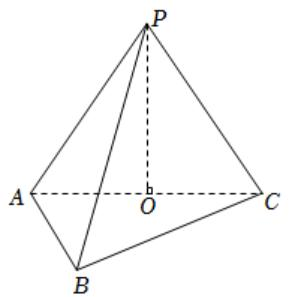
\includegraphics[width=.42\linewidth]{assets/asset-137-01.jpg}
\end{center}
\begin{solution}
\textbf{答案：}（1）$V_{P-ABC}=1$（2）$\arcsin\frac{\sqrt{3}}{4}$

\textbf{分析：}（1）直接利用体积公式求解；（2）以$D$为坐标原点，$DB$为$x$轴，$DC$为$y$轴，$DP$为$z$轴，建立空间直角坐标系，求得平面$PAC$的法向量，即可求解．

\textbf{详解：}解：（1）在三棱锥$P-ABC$中，因为$PD\perp$底面$ABC$，所以$PD\perp AB$，又$D$为$AB$边中点，所以$\triangle PAB$为等腰三角形，又$PA=PC=2$，所以$\triangle ABC$是边长为2的等边三角形，所以 $PD=\sqrt{3}$，三棱锥体积$V_{P-ABC}=\frac{1}{3}S_{\triangle ABC}\cdot PD=\frac{1}{3}\times\frac{\sqrt{3}}{4}\times2^2\times\sqrt{3}=1$．（2）以$D$为坐标原点，$DB$为$x$轴，$DC$为$y$轴，$DP$为$z$轴，建立空间直角坐标系，则$P(0,0,\sqrt{3})$，$B(\sqrt{3},0,0)$，$C(0,1,0)$，$M\left(\frac{\sqrt{3}}{2},\frac{1}{2},0\right)$，$\overrightarrow{DM}=\left(\frac{\sqrt{3}}{2},\frac{1}{2},-\sqrt{3}\right)$，平面$PAC$的法向量$\vec{n}=(\sqrt{3},0,0)$，设直线$DM$与平面$PAC$所成角为$\theta$，则$\sin\theta=\frac{|\overrightarrow{DM}\cdot\vec{n}|}{|\overrightarrow{DM}|\cdot|\vec{n}|}=\frac{\frac{3}{2}}{2\times\sqrt{3}}=\frac{\sqrt{3}}{4}$，所以$DM$与面$PAC$所成角大小为$\arcsin\frac{\sqrt{3}}{4}$．
\end{solution}
\end{question}

\begin{question}[points=5]
\textbf{来源：}2022 年 上海卷，第 3 题\par
如图正方体$ABCD-A_1B_1C_1D_1$中，$P$、$Q$、$R$、$S$分别为棱$AB$、$BC$、$BB_1$、$CD$的中点，联结$B_1D$，$B_1C$．空间任意两点$M$、$N$，若线段$MN$上不存在点在线段$B_1D$、$B_1C$上，则称$MN$两点可视，则下列选项中与点$B_1$可视的为（ ）

\begin{center}
  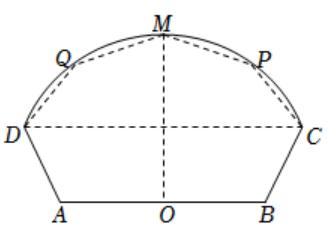
\includegraphics[width=.42\linewidth]{assets/asset-138-01.jpg}
\end{center}
\begin{choices}
  \item 点$P$
  \item 点$Q$
  \item 点$R$
  \item 点$S$
\end{choices}
\begin{solution}
\textbf{答案：}D

\textbf{分析：}线段$MN$上不存在点在线段$B_1D$、$B_1C$上，即直线$MN$与线段$B_1D$、$B_1C$不相交，因此所求与$B_1$可视的点，即求哪条线段不与线段$B_1D$、$B_1C$相交，再利用共面定理，异面直线的判定定理即可判断．

\textbf{详解：}解：线段$MN$上不存在点在线段$B_1D$、$B_1C$上，即直线$MN$与线段$B_1D$、$B_1C$不相交，因此所求与$B_1$可视的点，即求哪条线段不与线段$B_1D$、$B_1C$相交，对 A 选项，如图，连接$B_1P$、$BP$、$B_1Q$，因为$P$、$Q$分别为$AB$、$BC$的中点，所以 易证$B_1D_1//PQ$，故$B_1$、$D_1$、$P$、$Q$四点共面，所以 $B_1D$与$B_1P$相交，所以 A 错误；对 B、C 选项，如图，连接$B_1Q$、$BQ$，易证$B_1$、$Q$、$C$、$B$四点共面，故$B_1C$、$B_1Q$都与$B_1C$相交，所以 B、C 错误；对 D 选项，连接$B_1S$，由 A 选项分析知$B_1$、$D_1$、$P$、$Q$四点共面记为平面$B_1D_1PQ$，因为 $B_1\in$平面$B_1D_1PQ$，$S\notin$平面$B_1D_1PQ$，且$B_1D\subset$平面$B_1D_1PQ$，点$B_1\notin B_1D$，所以 $B_1S$与$B_1D$为异面直线，同理由 B，C 选项的分析知$B_1$、$Q$、$C$、$B$四点共面记为平面$B_1QCB$，因为 $B_1\in$平面$B_1QCB$，$S\notin$平面$B_1QCB$，且$B_1C\subset$平面$B_1QCB$，点$B_1\notin B_1C$，所以 $B_1S$与$B_1C$为异面直线，故$B_1S$与$B_1D$，$B_1C$都没有公共点，所以 D 选项正确．故选：D．
\end{solution}
\end{question}

\begin{question}[points=4]
\textbf{来源：}2022 年 上海卷，第 4 题\par
已知圆柱的高为 4，底面积为 $9\pi$，则圆柱的侧面积为 ．
\fillin[{$24\pi$}]
\begin{solution}
\textbf{答案：}$24\pi$

\textbf{分析：}由底面积为$9\pi$解出底面半径$r=3$，再代入侧面积公式求解即可．

\textbf{详解：}解：因为圆柱的底面积为$9\pi$，即$\pi r^2 =9\pi$，所以$r=3$，所以$S_{\text{侧}}=2\pi rh=24\pi$．故答案为：$24\pi$．
\end{solution}
\end{question}

\begin{question}[points=5]
\textbf{来源：}2022 年 天津卷，第 8 题\par
如图，“十字歇山”是由两个直三棱柱重叠后的景象，重叠后的底面为正方形，直三棱柱的底面是顶角为 $120^\circ$，腰为 $3$ 的等腰三角形，则该几何体的体积为（   ）

\begin{center}
  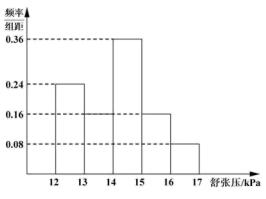
\includegraphics[width=.42\linewidth]{assets/asset-140-01.jpg}
\end{center}
\begin{choices}
  \item 23
  \item 24
  \item 26
  \item 27
\end{choices}
\begin{solution}
\textbf{答案：}27

\textbf{分析：}该几何体由直三棱柱 $AFD-BHC$ 及直三棱柱 $DGC-AEB$ 组成，作 $HM\perp CB$ 于 $M$，因为 $CH=BH=3,\angle CHB=120^\circ$，所以 $CM=BM=\frac{3\sqrt{3}}{2}, HM=\frac{3}{2}$。因为重叠后的底面为正方形，所以 $AB=BC=3\sqrt{3}$。在直棱柱 $AFD-BHC$ 中，$AB\perp$ 平面 $BHC$，则 $AB\perp HM$，由 $AB\cap BC=B$ 可得 $HM\perp$ 平面 $ADCB$。设重叠后的 $EG$ 与 $FH$ 交点为 $I$，则 $V_{I-BCDA}=\frac{1}{3}\times 3\sqrt{3}\times 3\sqrt{3}\times\frac{3}{2}=\frac{27}{2}$，$V_{AFD-BHC}=\frac{1}{2}\times 3\sqrt{3}\times\frac{3}{2}\times 3\sqrt{3}=\frac{81}{4}$，则该几何体的体积为 $V=2V_{AFD-BHC}-V_{I-BCDA}=2\times\frac{81}{4}-\frac{27}{2}=27$.
\end{solution}
\end{question}

\begin{question}[points=15]
\textbf{来源：}2022 年 天津卷，第 17 题\par
直三棱柱 $ABC-A_1B_1C_1$ 中，$AA_1=AB=AC=2$，$AA_1\perp AB$，$AC\perp AB$，$D$ 为 $A_1B_1$ 的中点，$E$ 为 $AA_1$ 的中点，$F$ 为 $CD$ 的中点．

（1）求证：$EF\parallel$ 平面 $ABC$；

（2）求直线 $BE$ 与平面 $CC_1D$ 所成角的正弦值；

（3）求平面 $A_1CD$ 与平面 $CC_1D$ 所成二面角的余弦值．
\begin{solution}
\textbf{答案：}（1）证明见解析；（2）$\frac{4}{5}$；（3）$\frac{\sqrt{10}}{10}$

\textbf{分析：}以点 $A_1$ 为坐标原点，$A_1A,A_1B_1,A_1C_1$ 所在直线分别为 $x,y,z$ 轴建立空间直角坐标系，利用空间向量法可证得结论和求解.

\textbf{详解：}（1）证明：在直三棱柱 $ABC-A_1B_1C_1$ 中，$AA_1\perp$ 平面 $A_1B_1C_1$，且 $AC\perp AB$，则 $A_1C_1\perp A_1B_1$，以点 $A_1$ 为坐标原点，$A_1A,A_1B_1,A_1C_1$ 所在直线分别为 $x,y,z$ 轴建立空间直角坐标系，则 $A(2,0,0),B(2,2,0),C(2,0,2),A_1(0,0,0),B_1(0,2,0),C_1(0,0,2),D(0,1,0),E(1,0,0),F(1,\frac{1}{2},1)$，$\overrightarrow{EF}=(0,\frac{1}{2},1)$，易知平面 $ABC$ 的一个法向量为 $\vec{m}=(1,0,0)$，则 $\overrightarrow{EF}\cdot\vec{m}=0$，故 $\overrightarrow{EF}\perp\vec{m}$，又 $EF\not\subset$ 平面 $ABC$，故 $EF\parallel$ 平面 $ABC$.
（2）$\overrightarrow{C_1C}=(2,0,0)$，$\overrightarrow{C_1D}=(0,1,-2)$，$\overrightarrow{EB}=(1,2,0)$，设平面 $CC_1D$ 的法向量为 $\vec{u}=(x_1,y_1,z_1)$，则 $\begin{cases} \vec{u}\cdot\overrightarrow{C_1C}=2x_1=0 \\ \vec{u}\cdot\overrightarrow{C_1D}=y_1-2z_1=0 \end{cases}$，取 $y_1=2$，得 $\vec{u}=(0,2,1)$，$\cos\langle\overrightarrow{EB},\vec{u}\rangle=\frac{\overrightarrow{EB}\cdot\vec{u}}{|\overrightarrow{EB}||\vec{u}|}=\frac{4}{5}$，故直线 $BE$ 与平面 $CC_1D$ 夹角的正弦值为 $\frac{4}{5}$.
（3）$\overrightarrow{A_1C}=(2,0,2)$，$\overrightarrow{A_1D}=(0,1,0)$，设平面 $A_1CD$ 的法向量为 $\vec{v}=(x_2,y_2,z_2)$，则 $\begin{cases} \vec{v}\cdot\overrightarrow{A_1C}=2x_2+2z_2=0 \\ \vec{v}\cdot\overrightarrow{A_1D}=y_2=0 \end{cases}$，取 $x_2=1$，得 $\vec{v}=(1,0,-1)$，$\cos\langle\vec{u},\vec{v}\rangle=\frac{\vec{u}\cdot\vec{v}}{|\vec{u}||\vec{v}|}=\frac{-1}{\sqrt{5}\times\sqrt{2}}=-\frac{\sqrt{10}}{10}$，故平面 $A_1CD$ 与平面 $CC_1D$ 夹角的余弦值为 $\frac{\sqrt{10}}{10}$.
\end{solution}
\end{question}

\begin{question}[points=5]
\textbf{来源：}2022 年 新高考II卷，第 7 题\par
已知正三棱台的高为1，上、下底面边长分别为$3\sqrt{3}$和$4\sqrt{3}$，其顶点都在同一球面上，则该球的表面积为（ ）
\begin{choices}
  \item $100\pi$
  \item $128\pi$
  \item $144\pi$
  \item $192\pi$
\end{choices}
\begin{solution}
\textbf{答案：}$100\pi$

\textbf{分析：}根据题意可求出正三棱台上下底面所在圆面的半径$r_1,r_2$，再根据球心距，圆面半径，以及球的半径之间的关系，即可解出球的半径，从而得出球的表面积.

\textbf{详解：}设正三棱台上下底面所在圆面的半径$r_1,r_2$，所以$2r_1=\dfrac{3\sqrt{3}}{\sin60^\circ},2r_2=\dfrac{4\sqrt{3}}{\sin60^\circ}$，即$r_1=3,r_2=4$，设球心到上下底面的距离分别为$d_1,d_2$，球的半径为$R$，所以$d_1=\sqrt{R^2-9},d_2=\sqrt{R^2-16}$，故$|d_1-d_2|=1$，即$\sqrt{R^2-9}-\sqrt{R^2-16}=1$或$\sqrt{R^2-9}+\sqrt{R^2-16}=1$，解得$R^2=25$符合题意，所以球的表面积为$S=4\pi R^2=100\pi$，故选A.
\end{solution}
\end{question}

\begin{question}[points=5]
\textbf{来源：}2022 年 新高考II卷，第 11 题\par
如图，四边形$ABCD$为正方形，$ED\perp$平面$ABCD$，$FB\parallel ED$，$AB=ED=2FB$，记三棱锥$E-ACD$，$F-ABC$，$F-ACE$的体积分别为$V_1,V_2,V_3$，则（ ）

\begin{center}
  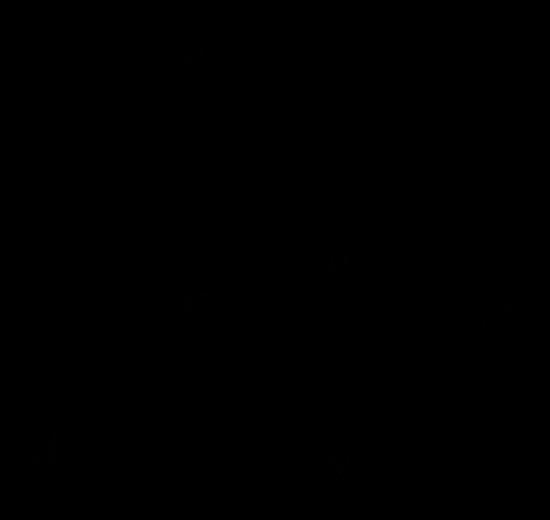
\includegraphics[width=.42\linewidth]{assets/asset-143-01.jpg}
\end{center}
\begin{choices}
  \item $V_3=2V_2$
  \item $V_3=V_1$
  \item $V_3=V_1+V_2$
  \item $2V_3=3V_1$
\end{choices}
\begin{solution}
\textbf{答案：}CD

\textbf{分析：}直接由体积公式计算$V_1,V_2$，连接$BD$交$AC$于点$M$，连接$EM,FM$，由$V_3=V_{A-EFM}+V_{C-EFM}$计算出$V_3$，依次判断选项即可.

\textbf{详解：}设$AB=ED=2FB=2a$，因为$ED\perp$平面$ABCD$，$FB\parallel ED$，则$V_1=\dfrac{1}{3}\cdot ED\cdot S_{\triangle ACD}=\dfrac{1}{3}\cdot 2a\cdot \dfrac{1}{2}\cdot(2a)^2=\dfrac{4}{3}a^3$，$V_2=\dfrac{1}{3}\cdot FB\cdot S_{\triangle ABC}=\dfrac{1}{3}\cdot a\cdot \dfrac{1}{2}\cdot (2a)^2=\dfrac{2}{3}a^3$，连接$BD$交$AC$于点$M$，连接$EM,FM$，易得$BD\perp AC$，又$ED\perp$平面$ABCD$，$AC\subset$平面$ABCD$，则$ED\perp AC$，又$ED\cap BD=D$，$ED,BD\subset$平面$BDEF$，则$AC\perp$平面$BDEF$，又$BM=DM=\dfrac{1}{2}BD=\sqrt{2}a$，过$F$作$FG\perp DE$于$G$，易得四边形$BDGF$为矩形，则$FG=BD=2\sqrt{2}a,EG=a$，则$EM=\sqrt{(\sqrt{2}a)^2+(\sqrt{2}a)^2}=2a,FM=\sqrt{a^2+(\sqrt{2}a)^2}=\sqrt{3}a,EF=\sqrt{a^2+(2\sqrt{2}a)^2}=3a$，$EM^2+FM^2=EF^2$，则$EM\perp FM$，$S_{\triangle EFM}=\dfrac{1}{2}EM\cdot FM=\dfrac{1}{2}\cdot 2a\cdot\sqrt{3}a=\sqrt{3}a^2$，$AC=2\sqrt{2}a$，则$V_3=V_{A-EFM}+V_{C-EFM}=\dfrac{1}{3}AC\cdot S_{\triangle EFM}=2a^3$，则$2V_3=3V_1$，$V_3=3V_2$，$V_3=V_1+V_2$，故AB错误；CD正确. 故选CD.
\end{solution}
\end{question}

\begin{question}[points=12]
\textbf{来源：}2022 年 新高考II卷，第 20 题\par
如图，$PO$是三棱锥$P-ABC$的高，$PA=PB$，$AB\perp AC$，$E$是$PB$的中点．

(1)证明：$OE\parallel$平面$PAC$；

(2)若$\angle ABO=\angle CBO=30^\circ$，$PO=3$，$PA=5$，求二面角$C-AE-B$的正弦值．

\begin{center}
  
\includegraphics[width=.42\linewidth]{assets/asset-144-01.jpg}
\end{center}
\begin{solution}
\textbf{答案：}（1）证明见解析；（2）$\dfrac{11}{13}$

\textbf{分析：}（1）连接$BO$并延长交$AC$于点$D$，连接$OA,PD$，根据三角形全等得到$OA=OB$，再根据直角三角形的性质得到$AO=DO$，即可得到$O$为$BD$的中点从而得到$OE\parallel PD$，即可得证；（2）建立适当的空间直角坐标系，利用空间向量法求出二面角的余弦的绝对值，再根据同角三角函数的基本关系计算可得.

\textbf{详解：}（1）证明：连接$BO$并延长交$AC$于点$D$，连接$OA,PD$，因为$PO$是三棱锥$P-ABC$的高，所以$PO\perp$平面$ABC$，$AO,BO\subset$平面$ABC$，所以$PO\perp AO,PO\perp BO$，又$PA=PB$，所以$\triangle POA\cong\triangle POB$，即$OA=OB$，所以$\angle OAB=\angle OBA$，又$AB\perp AC$，即$\angle BAC=90^\circ$，所以$\angle OAB+\angle OAD=90^\circ$，$\angle OBA+\angle ODA=90^\circ$，所以$\angle ODA=\angle OAD$，所以$AO=DO$，即$AO=DO=OB$，所以$O$为$BD$的中点，又$E$为$PB$的中点，所以$OE\parallel PD$，又$OE\not\subset$平面$PAC$，$PD\subset$平面$PAC$，所以$OE\parallel$平面$PAC$．
（2）解：过点$A$作$Az\parallel OP$，如图建立平面直角坐标系，因为$PO=3$，$AP=5$，所以$OA=\sqrt{AP^2-PO^2}=4$，又$\angle OBA=\angle OBC=30^\circ$，所以$BD=2OA=8$，则$AD=4$，$AB=4\sqrt{3}$，所以$AC=12$，所以$O(2\sqrt{3},2,0)$，$B(4\sqrt{3},0,0)$，$P(2\sqrt{3},2,3)$，$C(0,12,0)$，所以$E(3\sqrt{3},1,\dfrac{3}{2})$，则$\overrightarrow{AE}=(3\sqrt{3},1,\dfrac{3}{2})$，$\overrightarrow{AB}=(4\sqrt{3},0,0)$，$\overrightarrow{AC}=(0,12,0)$，设平面$AEB$的法向量为$\vec{n}=(x,y,z)$，则$\begin{cases} \vec{n}\cdot\overrightarrow{AE}=3\sqrt{3}x+y+\dfrac{3}{2}z=0 \\ \vec{n}\cdot\overrightarrow{AB}=4\sqrt{3}x=0 \end{cases}$，令$z=2$，则$y=-3$，$x=0$，所以$\vec{n}=(0,-3,2)$；设平面$AEC$的法向量为$\vec{m}=(a,b,c)$，则$\begin{cases} \vec{m}\cdot\overrightarrow{AE}=3\sqrt{3}a+b+\dfrac{3}{2}c=0 \\ \vec{m}\cdot\overrightarrow{AC}=12b=0 \end{cases}$，令$a=\sqrt{3}$，则$c=-6$，$b=0$，所以$\vec{m}=(\sqrt{3},0,-6)$；所以$\cos\langle\vec{n},\vec{m}\rangle=\dfrac{\vec{n}\cdot\vec{m}}{|\vec{n}||\vec{m}|}=\dfrac{-12}{\sqrt{13}\times\sqrt{39}}=-\dfrac{4\sqrt{3}}{13}$．设二面角$C-AE-B$的大小为$\theta$，则$\cos\theta=|\cos\langle\vec{n},\vec{m}\rangle|=\dfrac{4\sqrt{3}}{13}$，所以$\sin\theta=\sqrt{1-\cos^2\theta}=\sqrt{1-\left(\dfrac{4\sqrt{3}}{13}\right)^2}=\dfrac{11}{13}$，即二面角$C-AE-B$的正弦值为$\dfrac{11}{13}$.
\end{solution}
\end{question}

\begin{question}[points=5]
\textbf{来源：}2022 年 新高考I卷，第 4 题\par
南水北调工程缓解了北方一些地区水资源短缺问题, 其中一部分水蓄入某水库. 已知该水库水位为海拔 $148.5\,\mathrm{m}$ 时, 相应水面的面积为 $140.0\,\mathrm{km}^2$; 水位为海拔 $157.5\,\mathrm{m}$ 时, 相应水面的面积为 $180.0\,\mathrm{km}^2$, 将该水库在这两个水位间的形状看作一个棱台, 则该水库水位从海拔 $148.5\,\mathrm{m}$ 上升到 $157.5\,\mathrm{m}$ 时, 增加的水量约为 ($\sqrt{7} \approx 2.65$)
\begin{choices}
  \item $1.0 \times 10^9\,\mathrm{m}^3$
  \item $1.2 \times 10^9\,\mathrm{m}^3$
  \item $1.4 \times 10^9\,\mathrm{m}^3$
  \item $1.6 \times 10^9\,\mathrm{m}^3$
\end{choices}
\begin{solution}
\textbf{答案：}C

\textbf{分析：}根据题意只要求出棱台的高, 即可利用棱台的体积公式求出.

\textbf{详解：}依题意可知棱台的高为 $MN = 157.5 - 148.5 = 9\,(\mathrm{m})$, 所以增加的水量即为棱台的体积 $V$. 棱台上底面积 $S = 140.0\,\mathrm{km}^2 = 140 \times 10^6\,\mathrm{m}^2$, 下底面积 $S' = 180.0\,\mathrm{km}^2 = 180 \times 10^6\,\mathrm{m}^2$, $\therefore V = \frac{1}{3}h(S + S' + \sqrt{SS'}) = \frac{1}{3} \times 9 \times (140 \times 10^6 + 180 \times 10^6 + \sqrt{140 \times 180} \times 10^6) = 3 \times (320 + 60\sqrt{7}) \times 10^6 \approx (96 + 18 \times 2.65) \times 10^7 = 1.437 \times 10^9 \approx 1.4 \times 10^9\,(\mathrm{m}^3)$.
\end{solution}
\end{question}

\begin{question}[points=5]
\textbf{来源：}2022 年 新高考I卷，第 8 题\par
已知正四棱锥的侧棱长为 $l$, 其各顶点都在同一球面上. 若该球的体积为 $36\pi$, 且 $3 \le l \le 3\sqrt{3}$, 则该正四棱锥体积的取值范围是
\begin{choices}
  \item $\left[18, \frac{81}{4}\right]$
  \item $\left[\frac{27}{4}, \frac{81}{4}\right]$
  \item $\left[\frac{27}{4}, \frac{64}{3}\right]$
  \item $[18, 27]$
\end{choices}
\begin{solution}
\textbf{答案：}C

\textbf{分析：}设正四棱锥的高为 $h$, 由球的截面性质列方程求出正四棱锥的底面边长与高的关系, 由此确定正四棱锥体积的取值范围.

\textbf{详解：}球的体积为 $36\pi$, 所以球的半径 $R=3$. 设正四棱锥的底面边长为 $2a$, 高为 $h$, 则 $l^2 = 2a^2 + h^2$, $3^2 = 2a^2 + (3-h)^2$, 所以 $6h = l^2$, $2a^2 = l^2 - h^2$. 所以正四棱锥的体积 $V = \frac{1}{3}Sh = \frac{1}{3} \times 4a^2 \times h = \frac{1}{3} \times (l^2 - \frac{l^4}{36}) \times \frac{l^2}{6} = \frac{1}{9}\left(l^4 - \frac{l^6}{36}\right)$. 所以 $V' = \frac{1}{9}\left(4l^3 - \frac{5l^5}{6}\right) = \frac{1}{9}l^3\left(4 - \frac{5l^2}{6}\right) = \frac{1}{9}l^3\frac{24 - 5l^2}{6}$. 当 $3 \le l < 2\sqrt{6}$ 时, $V' > 0$; 当 $2\sqrt{6} < l \le 3\sqrt{3}$ 时, $V' < 0$. 所以当 $l = 2\sqrt{6}$ 时, $V$ 取最大值 $\frac{64}{3}$. 又 $l=3$ 时, $V = \frac{27}{4}$; $l=3\sqrt{3}$ 时, $V = \frac{81}{4}$. 所以体积的最小值为 $\frac{27}{4}$. 所以该正四棱锥体积的取值范围是 $\left[\frac{27}{4}, \frac{64}{3}\right]$.
\end{solution}
\end{question}

\begin{question}[points=5]
\textbf{来源：}2022 年 新高考I卷，第 9 题\par
已知正方体 $ABCD - A_1B_1C_1D_1$, 则
\begin{choices}
  \item 直线 $BC_1$ 与 $DA_1$ 所成的角为 $90^\circ$
  \item 直线 $BC_1$ 与 $CA_1$ 所成的角为 $90^\circ$
  \item 直线 $BC_1$ 与平面 $BB_1D_1D$ 所成的角为 $45^\circ$
  \item 直线 $BC_1$ 与平面 $ABCD$ 所成的角为 $45^\circ$
\end{choices}
\begin{solution}
\textbf{答案：}ABD

\textbf{分析：}数形结合, 依次对所给选项进行判断即可.

\textbf{详解：}如图, 连接 $B_1C$, $BC_1$, 因为 $DA_1 /\!\! / B_1C$, 所以直线 $BC_1$ 与 $B_1C$ 所成的角即为直线 $BC_1$ 与 $DA_1$ 所成的角. 因为四边形 $BB_1C_1C$ 为正方形, 则 $B_1C \perp BC_1$, 故直线 $BC_1$ 与 $DA_1$ 所成的角为 $90^\circ$, A 正确. 连接 $A_1C$, 因为 $A_1B_1 \perp$ 平面 $BB_1C_1C$, $BC_1 \subset$ 平面 $BB_1C_1C$, 则 $A_1B_1 \perp BC_1$. 因为 $B_1C \perp BC_1$, $A_1B_1 \cap B_1C = B_1$, 所以 $BC_1 \perp$ 平面 $A_1B_1C$. 又 $A_1C \subset$ 平面 $A_1B_1C$, 所以 $BC_1 \perp CA_1$, 故 B 正确. 连接 $A_1C_1$, 设 $A_1C_1 \cap B_1D_1 = O$, 连接 $BO$. 因为 $BB_1 \perp$ 平面 $A_1B_1C_1D_1$, $C_1O \subset$ 平面 $A_1B_1C_1D_1$, 则 $C_1O \perp B_1B$. 因为 $C_1O \perp B_1D_1$, $B_1D_1 \cap B_1B = B_1$, 所以 $C_1O \perp$ 平面 $BB_1D_1D$. 所以 $\angle C_1BO$ 为直线 $BC_1$ 与平面 $BB_1D_1D$ 所成的角. 设正方体棱长为 1, 则 $C_1O = \frac{\sqrt{2}}{2}$, $BC_1 = \sqrt{2}$, $\sin\angle C_1BO = \frac{C_1O}{BC_1} = \frac{1}{2}$, 所以直线 $BC_1$ 与平面 $BB_1D_1D$ 所成的角为 $30^\circ$, 故 C 错误. 因为 $C_1C \perp$ 平面 $ABCD$, 所以 $\angle C_1BC$ 为直线 $BC_1$ 与平面 $ABCD$ 所成的角, 易得 $\angle C_1BC = 45^\circ$, 故 D 正确.
\end{solution}
\end{question}

\begin{question}[points=12]
\textbf{来源：}2022 年 新高考I卷，第 19 题\par
如图, 直三棱柱 $ABC - A_1B_1C_1$ 的体积为 $4$, $\triangle A_1BC$ 的面积为 $2\sqrt{2}$.

(1) 求 $A$ 到平面 $A_1BC$ 的距离;

(2) 设 $D$ 为 $A_1C$ 的中点, $AA_1 = AB$, 平面 $A_1BC \perp$ 平面 $ABB_1A_1$, 求二面角 $A - BD - C$ 的正弦值.
\begin{solution}
\textbf{答案：}(1) $\sqrt{2}$; (2) $\frac{\sqrt{3}}{2}$

\textbf{分析：}(1) 由等体积法运算即可得解. (2) 由面面垂直的性质及判定可得 $BC \perp$ 平面 $ABB_1A_1$, 建立空间直角坐标系, 利用空间向量法即可得解.

\textbf{详解：}(1) 在直三棱柱 $ABC - A_1B_1C_1$ 中, 设点 $A$ 到平面 $A_1BC$ 的距离为 $h$, 则 $V_{A-A_1BC} = \frac{1}{3}S_{\triangle A_1BC} \cdot h = \frac{2\sqrt{2}}{3}h = V_{A_1-ABC} = \frac{1}{3}S_{\triangle ABC} \cdot A_1A = \frac{1}{3}V_{ABC-A_1B_1C_1} = \frac{4}{3}$, 解得 $h = \sqrt{2}$.
(2) 取 $A_1B$ 的中点 $E$, 连接 $AE$. 因为 $AA_1 = AB$, 所以 $AE \perp A_1B$. 又平面 $A_1BC \perp$ 平面 $ABB_1A_1$, 平面 $A_1BC \cap$ 平面 $ABB_1A_1 = A_1B$, 且 $AE \subset$ 平面 $ABB_1A_1$, 所以 $AE \perp$ 平面 $A_1BC$. 在直三棱柱 $ABC - A_1B_1C_1$ 中, $BB_1 \perp$ 平面 $ABC$. 由 $BC \subset$ 平面 $A_1BC$, $BC \subset$ 平面 $ABC$ 可得 $AE \perp BC$, $BB_1 \perp BC$. 又 $AE$, $BB_1 \subset$ 平面 $ABB_1A_1$ 且相交, 所以 $BC \perp$ 平面 $ABB_1A_1$. 所以 $BC$, $BA$, $BB_1$ 两两垂直. 以 $B$ 为原点, 建立空间直角坐标系. 由 (1) 得 $AE = \sqrt{2}$, 所以 $AA_1 = AB = 2$, $A_1B = 2\sqrt{2}$, $BC = 2$. 则 $A(0,2,0)$, $A_1(0,2,2)$, $B(0,0,0)$, $C(2,0,0)$, $A_1C$ 的中点 $D(1,1,1)$. $\overrightarrow{BD} = (1,1,1)$, $\overrightarrow{BA} = (0,2,0)$, $\overrightarrow{BC} = (2,0,0)$. 设平面 $ABD$ 的一个法向量 $\vec{m} = (x,y,z)$, 则 $\begin{cases} \vec{m} \cdot \overrightarrow{BD} = x + y + z = 0 \\ \vec{m} \cdot \overrightarrow{BA} = 2y = 0 \end{cases}$, 可取 $\vec{m} = (1,0,-1)$. 设平面 $BDC$ 的一个法向量 $\vec{n} = (a,b,c)$, 则 $\begin{cases} \vec{n} \cdot \overrightarrow{BD} = a + b + c = 0 \\ \vec{n} \cdot \overrightarrow{BC} = 2a = 0 \end{cases}$, 可取 $\vec{n} = (0,1,-1)$. 则 $\cos\langle\vec{m},\vec{n}\rangle = \frac{\vec{m} \cdot \vec{n}}{|\vec{m}| |\vec{n}|} = \frac{1}{\sqrt{2} \times \sqrt{2}} = \frac{1}{2}$, 所以二面角 $A - BD - C$ 的正弦值为 $\sqrt{1 - \left(\frac{1}{2}\right)^2} = \frac{\sqrt{3}}{2}$.
\end{solution}
\end{question}

\begin{question}[points=4]
\textbf{来源：}2022 年 浙江卷，第 5 题\par
某几何体的三视图如图所示（单位：$\mathrm{cm}$），则该几何体的体积（单位：$\mathrm{cm}^3$）是（ ）

\begin{center}
  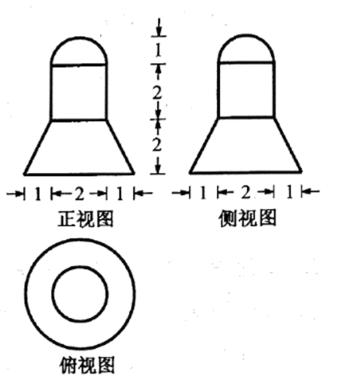
\includegraphics[width=.42\linewidth]{assets/asset-149-01.jpg}
\end{center}
\begin{choices}
  \item $22\pi$
  \item $8\pi$
  \item $\dfrac{22}{3}\pi$
  \item $\dfrac{16}{3}\pi$
\end{choices}
\begin{solution}
\textbf{答案：}C

\textbf{分析：}根据三视图还原几何体可知，原几何体是一个半球，一个圆柱，一个圆台组合成的几何体，即可根据球，圆柱，圆台的体积公式求出．

\textbf{详解：}由三视图可知，该几何体是一个半球，一个圆柱，一个圆台组合成的几何体，球的半径、圆柱的底面半径、圆台的上底面半径都为 $1\mathrm{cm}$，圆台的下底面半径为 $2\mathrm{cm}$，所以体积 $V = \frac{1}{2} \times \frac{4}{3}\pi \times 1^3 + \pi \times 1^2 \times 2 + \frac{1}{3} \times 2 \times [\pi \times 2^2 + \pi \times 1^2 + \sqrt{\pi \times 2^2 \times \pi \times 1^2}] = \frac{22}{3}\pi \mathrm{cm}^3$，故选C.
\end{solution}
\end{question}

\begin{question}[points=4]
\textbf{来源：}2022 年 浙江卷，第 8 题\par
如图，已知正三棱柱 $ABC-A_1B_1C_1, AC = AA_1$，$E,F$ 分别是棱 $BC, A_1C_1$ 上的点．记 $EF$ 与 $AA_1$ 所成的角为 $\alpha$，$EF$ 与平面 $ABC$ 所成的角为 $\beta$，二面角 $F-BC-A$ 的平面角为 $\gamma$，则（ ）
\begin{choices}
  \item $\alpha \le \beta \le \gamma$
  \item $\beta \le \alpha \le \gamma$
  \item $\beta \le \gamma \le \alpha$
  \item $\alpha \le \gamma \le \beta$
\end{choices}
\begin{solution}
\textbf{答案：}A

\textbf{分析：}先用几何法表示出 $\alpha,\beta,\gamma$，再根据边长关系即可比较大小．

\textbf{详解：}如图所示，过点 $F$ 作 $FP \perp AC$ 于 $P$，过 $P$ 作 $PM \perp BC$ 于 $M$，连接 $PE$，则 $\alpha = \angle EFP$，$\beta = \angle FEP$，$\gamma = \angle FMP$，$\tan\alpha = \frac{PE}{FP} \le 1$，$\tan\beta = \frac{FP}{PE} \ge 1$，$\tan\gamma = \frac{FP}{PM} \ge \frac{FP}{PE} = \tan\beta$，所以 $\alpha \le \beta \le \gamma$，故选A.
\end{solution}
\end{question}

\begin{question}[points=15]
\textbf{来源：}2022 年 浙江卷，第 19 题\par
如图，已知 $ABCD$ 和 $CDEF$ 都是直角梯形，$AB\parallel DC, DC\parallel EF, AB=5, DC=3, EF=1, \angle BAD = \angle CDE = 60^\circ$，二面角 $F-DC-B$ 的平面角为 $60^\circ$．设 $M,N$ 分别为 $AE, BC$ 的中点．

（1）证明：$FN \perp AD$；

（2）求直线 $BM$ 与平面 $ADE$ 所成角的正弦值．
\begin{solution}
\textbf{答案：}（1）见解析；（2）$\dfrac{5\sqrt{7}}{14}$

\textbf{分析：}（1）过点 $E,D$ 分别做直线 $DC,AB$ 的垂线 $EG,DH$，由平面几何知识易得 $FC=BC$，再根据二面角的定义可知 $\angle BCF=60^\circ$，由此可证得 $FN\perp$ 平面 $ABCD$，即得 $FN\perp AD$；（2）建立空间直角坐标系，利用线面角的向量公式求解．

\textbf{详解：}（1）过 $E$ 作 $EG\perp DC$ 于 $G$，过 $D$ 作 $DH\perp AB$ 于 $H$，易得 $DG=AH=2$，$\angle EFC = \angle DCF = \angle DCB = \angle ABC = 90^\circ$，所以 $EG=DH=2\sqrt{3}$．由 $DC\perp CF, DC\perp CB$ 得 $DC\perp$ 平面 $BCF$，所以 $\angle BCF=60^\circ$，$\triangle BCF$ 是正三角形．$N$ 是 $BC$ 中点，故 $FN\perp BC$，又 $DC\perp$ 平面 $BCF$，$FN\subset$ 平面 $BCF$，故 $FN\perp CD$，所以 $FN\perp$ 平面 $ABCD$，则 $FN\perp AD$．
（2）以 $N$ 为原点，$NK$（平行 $AB$）、$NB$、$NF$ 分别为 $x,y,z$ 轴建立空间直角坐标系，则 $A(5,\sqrt{3},0), B(0,\sqrt{3},0), D(3,-\sqrt{3},0), E(1,0,3)$，$M\left(3,\frac{\sqrt{3}}{2},\frac{3}{2}\right)$，$\overrightarrow{BM} = \left(3,-\frac{\sqrt{3}}{2},\frac{3}{2}\right)$，$\overrightarrow{AD}=(-2,-2\sqrt{3},0)$，$\overrightarrow{DE}=(-2,\sqrt{3},3)$．设平面 $ADE$ 的法向量为 $\mathbf{n}=(x,y,z)$，由 $\mathbf{n}\cdot\overrightarrow{AD}=0$ 且 $\mathbf{n}\cdot\overrightarrow{DE}=0$ 得 $\begin{cases} -2x-2\sqrt{3}y=0 \\ -2x+\sqrt{3}y+3z=0 \end{cases}$，取 $\mathbf{n}=(\sqrt{3},-1,\sqrt{3})$．设 $BM$ 与平面 $ADE$ 所成角为 $\theta$，则 $\sin\theta = \frac{|\mathbf{n}\cdot\overrightarrow{BM}|}{|\mathbf{n}|\cdot|\overrightarrow{BM}|} = \frac{|3\sqrt{3}+\frac{\sqrt{3}}{2}+\frac{3\sqrt{3}}{2}|}{\sqrt{3+1+3}\cdot\sqrt{9+\frac{3}{4}+\frac{9}{4}}} = \frac{5\sqrt{7}}{14}$.
\end{solution}
\end{question}

\section*{2023 年}

\begin{question}[points=4]
\textbf{来源：}2023 年 北京卷，第 9 题\par
坡屋顶是我国传统建筑造型之一，蕴含着丰富的数学元素．安装灯带可以勾勒出建筑轮廓，展现造型之美．如图，某坡屋顶可视为一个五面体，其中两个面是全等的等腰梯形，两个面是全等的等腰三角形．若 $AB = 25\text{m}, BC = AD = 10\text{m}$ ，且等腰梯形所在的平面、等腰三角形所在的平面与平面 $ABCD$ 的夹角的正切值均为 $\dfrac{\sqrt{14}}{5}$ ，则该五面体的所有棱长之和为（ ）

\begin{center}
  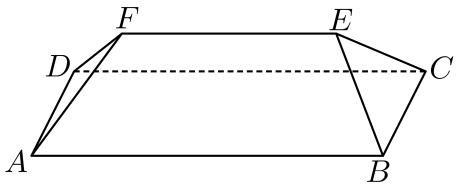
\includegraphics[width=.42\linewidth]{assets/asset-152-01.jpg}
\end{center}
\begin{choices}
  \item $102\text{m}$
  \item $112\text{m}$
  \item $117\text{m}$
  \item $125\text{m}$
\end{choices}
\begin{solution}
\textbf{答案：}C

\textbf{分析：}先根据线面角的定义求得 $\tan\angle EMO = \tan\angle EGO = \frac{\sqrt{14}}{5}$，从而依次求 $EO, EG, EB, EF$，再把所有棱长相加即可得解.

\textbf{详解：}如图，过 $E$ 做 $EO \perp$ 平面 $ABCD$，垂足为 $O$，过 $E$ 分别做 $EG \perp BC$，$EM \perp AB$，垂足分别为 $G, M$，连接 $OG, OM$。由题意得等腰梯形所在的面、等腰三角形所在的面与底面夹角分别为 $\angle EMO$ 和 $\angle EGO$，所以 $\tan\angle EMO = \tan\angle EGO = \frac{\sqrt{14}}{5}$。因为 $EO \perp$ 平面 $ABCD$，$BC \subset$ 平面 $ABCD$，所以 $EO \perp BC$，因为 $EG \perp BC$，$EO, EG \subset$ 平面 $EOG$，$EO \cap EG = E$，所以 $BC \perp$ 平面 $EOG$，因为 $OG \subset$ 平面 $EOG$，所以 $BC \perp OG$。同理：$OM \perp BM$，又 $BM \perp BG$，故四边形 $OMBG$ 是矩形，所以由 $BC=10$ 得 $OM=5$，所以 $EO = \sqrt{14}$，所以 $OG=5$，所以在直角三角形 $EOG$ 中，$EG = \sqrt{EO^2+OG^2} = \sqrt{(\sqrt{14})^2+5^2} = \sqrt{39}$，在直角三角形 $EBG$ 中，$BG=OM=5$，$EB = \sqrt{EG^2+BG^2} = \sqrt{(\sqrt{39})^2+5^2} = 8$，又因为 $EF = AB - 5 - 5 = 25-5-5=15$，所有棱长之和为 $2\times25 + 2\times10 + 15 + 4\times8 = 117$ m.
\end{solution}
\end{question}

\begin{question}[points=14]
\textbf{来源：}2023 年 北京卷，第 16 题\par
如图，在三棱锥 $P-ABC$ 中，$PA\perp$ 平面 $ABC$，$PA=AB=BC=1$，$PC=\sqrt{3}$．

（1）求证：$BC\perp$ 平面 $PAB$；

（2）求二面角 $A-PC-B$ 的大小．
\begin{solution}
\textbf{答案：}（1）证明见解析 （2）$\dfrac{\pi}{3}$

\textbf{分析：}（1）先由线面垂直的性质证得 $PA\perp BC$，再利用勾股定理证得 $BC\perp PB$，从而利用线面垂直的判定定理即可得证；（2）结合（1）中结论，建立空间直角坐标系，分别求得平面$PAC$与平面$PBC$的法向量，再利用空间向量夹角余弦的坐标表示即可得解.

\textbf{详解：}（1）因为 $PA\perp$ 平面 $ABC$，$BC\subset$ 平面 $ABC$，所以 $PA\perp BC$，同理 $PA\perp AB$，所以 $\triangle PAB$ 为直角三角形。又因为 $PB=\sqrt{PA^2+AB^2}=\sqrt{2}$，$BC=1$，$PC=\sqrt{3}$，所以 $PB^2+BC^2=PC^2$，则 $\triangle PBC$ 为直角三角形，故 $BC\perp PB$。又因为 $BC\perp PA$，$PA\cap PB=P$，所以 $BC\perp$ 平面 $PAB$。
（2）由（1）$BC\perp$ 平面 $PAB$，又 $AB\subset$ 平面 $PAB$，则 $BC\perp AB$。以 $A$ 为原点，$AB$ 为 $x$ 轴，过 $A$ 且与 $BC$ 平行的直线为 $y$ 轴，$AP$ 为 $z$ 轴，建立空间直角坐标系，如图，则 $A(0,0,0), P(0,0,1), C(1,1,0), B(1,0,0)$，所以 $\overrightarrow{AP}=(0,0,1), \overrightarrow{AC}=(1,1,0), \overrightarrow{BC}=(0,1,0), \overrightarrow{PC}=(1,1,-1)$。设平面 $PAC$ 的法向量为 $\vec{m}=(x_1,y_1,z_1)$，则 $\begin{cases} \vec{m}\cdot\overrightarrow{AP}=0 \\ \vec{m}\cdot\overrightarrow{AC}=0 \end{cases}$，即 $\begin{cases} z_1=0 \\ x_1+y_1=0 \end{cases}$，令 $x_1=1$，则 $y_1=-1$，所以 $\vec{m}=(1,-1,0)$。设平面 $PBC$ 的法向量为 $\vec{n}=(x_2,y_2,z_2)$，则 $\begin{cases} \vec{n}\cdot\overrightarrow{BC}=0 \\ \vec{n}\cdot\overrightarrow{PC}=0 \end{cases}$，即 $\begin{cases} y_2=0 \\ x_2+y_2-z_2=0 \end{cases}$，令 $x_2=1$，则 $z_2=1$，所以 $\vec{n}=(1,0,1)$。所以 $\cos\langle\vec{m},\vec{n}\rangle = \frac{\vec{m}\cdot\vec{n}}{|\vec{m}||\vec{n}|} = \frac{1}{\sqrt{2}\times\sqrt{2}} = \frac12$。又因为二面角 $A-PC-B$ 为锐二面角，所以二面角 $A-PC-B$ 的大小为 $\frac{\pi}{3}$.
\end{solution}
\end{question}

\begin{question}[points=5]
\textbf{来源：}2023 年 全国甲卷-理科，第 11 题\par
已知四棱锥 $P-ABCD$ 的底面是边长为 4 的正方形，$PC = PD = 3$，$\angle PCA = 45^\circ$，则 $\triangle PBC$ 的面积为（         ）
\begin{choices}
  \item $2\sqrt{2}$
  \item $3\sqrt{2}$
  \item $4\sqrt{2}$
  \item $6\sqrt{2}$
\end{choices}
\begin{solution}
\textbf{答案：}C

\textbf{分析：}法一：利用全等三角形的证明方法依次证得 $\triangle PDO \cong \triangle PCO$，$\triangle PDB \cong \triangle PCA$，从而得到 $PA = PB$，再在 $\triangle PAC$ 中利用余弦定理求得 $PA = \sqrt{17}$，从而求得 $PB = \sqrt{17}$，由此在 $\triangle PBC$ 中利用余弦定理与三角形面积公式即可得解；法二：先在 $\triangle PAC$ 中利用余弦定理求得 $PA = \sqrt{17}$，$\cos \angle PCB = \frac{1}{3}$，从而求得 $\overrightarrow{PA}\cdot\overrightarrow{PC} = -3$，再利用空间向量的数量积运算与余弦定理得到关于 $PB$，$\angle BPD$ 的方程组，从而求得 $PB = \sqrt{17}$，由此在 $\triangle PBC$ 中利用余弦定理与三角形面积公式即可得解．

\textbf{详解：}法一：连结 $AC$，$BD$ 交于 $O$，连结 $PO$，则 $O$ 为 $AC$，$BD$ 的中点，因为底面 $ABCD$ 为正方形，$AB=4$，所以 $AC=BD=4\sqrt{2}$，则 $DO=CO=2\sqrt{2}$，又 $PC=PD=3$，$PO=OP$，所以 $\triangle PDO \cong \triangle PCO$，则 $\angle PDO = \angle PCO$，又 $PC=PD=3$，$AC=BD=4\sqrt{2}$，所以 $\triangle PDB \cong \triangle PCA$，则 $PA=PB$，在 $\triangle PAC$ 中，$PC=3$，$AC=4\sqrt{2}$，$\angle PCA = 45^\circ$，则由余弦定理可得 $PA^2 = AC^2 + PC^2 - 2AC\cdot PC\cos\angle PCA = 32+9-2\times4\sqrt{2}\times3\times\frac{\sqrt{2}}{2}=17$，故 $PA=\sqrt{17}$，则 $PB=\sqrt{17}$，故在 $\triangle PBC$ 中，$PC=3$，$PB=\sqrt{17}$，$BC=4$，所以 $\cos\angle PCB = \frac{PC^2+BC^2-PB^2}{2PC\cdot BC} = \frac{9+16-17}{2\times3\times4} = \frac{1}{3}$，又 $0<\angle PCB<\pi$，所以 $\sin\angle PCB = \sqrt{1-\cos^2\angle PCB} = \frac{2\sqrt{2}}{3}$，所以 $\triangle PBC$ 的面积为 $S = \frac{1}{2} PC\cdot BC\sin\angle PCB = \frac{1}{2}\times3\times4\times\frac{2\sqrt{2}}{3} = 4\sqrt{2}$．
法二：连结 $AC$，$BD$ 交于 $O$，连结 $PO$，则 $O$ 为 $AC$，$BD$ 的中点，因为底面 $ABCD$ 为正方形，$AB=4$，所以 $AC=BD=4\sqrt{2}$，在 $\triangle PAC$ 中，$PC=3$，$\angle PCA = 45^\circ$，则由余弦定理可得 $PA^2 = AC^2+PC^2-2AC\cdot PC\cos\angle PCA = 32+9-2\times4\sqrt{2}\times3\times\frac{\sqrt{2}}{2}=17$，故 $PA=\sqrt{17}$，所以 $\cos\angle APC = \frac{PA^2+PC^2-AC^2}{2PA\cdot PC} = \frac{17+9-32}{2\times\sqrt{17}\times3} = -\frac{\sqrt{17}}{17}$，则 $\overrightarrow{PA}\cdot\overrightarrow{PC} = |\overrightarrow{PA}||\overrightarrow{PC}|\cos\angle APC = \sqrt{17}\times3\times\left(-\frac{\sqrt{17}}{17}\right) = -3$，不妨记 $PB=m$，$\angle BPD = \theta$，因为 $\overrightarrow{PO} = \frac{1}{2}(\overrightarrow{PA}+\overrightarrow{PC}) = \frac{1}{2}(\overrightarrow{PB}+\overrightarrow{PD})$，所以 $(\overrightarrow{PA}+\overrightarrow{PC})^2 = (\overrightarrow{PB}+\overrightarrow{PD})^2$，即 $|\overrightarrow{PA}|^2+|\overrightarrow{PC}|^2+2\overrightarrow{PA}\cdot\overrightarrow{PC} = |\overrightarrow{PB}|^2+|\overrightarrow{PD}|^2+2\overrightarrow{PB}\cdot\overrightarrow{PD}$，则 $17+9+2\times(-3) = m^2+9+2\times3\times m\cos\theta$，整理得 $m^2+6m\cos\theta-11=0$ ①，又在 $\triangle PBD$ 中，$BD^2 = PB^2+PD^2-2PB\cdot PD\cos\angle BPD$，即 $32 = m^2+9-6m\cos\theta$，则 $m^2-6m\cos\theta-23=0$ ②，两式相加得 $2m^2-34=0$，故 $PB=m=\sqrt{17}$，故在 $\triangle PBC$ 中，$PC=3$，$PB=\sqrt{17}$，$BC=4$，所以 $\cos\angle PCB = \frac{PC^2+BC^2-PB^2}{2PC\cdot BC} = \frac{9+16-17}{2\times3\times4} = \frac{1}{3}$，又 $0<\angle PCB<\pi$，所以 $\sin\angle PCB = \sqrt{1-\cos^2\angle PCB} = \frac{2\sqrt{2}}{3}$，所以 $\triangle PBC$ 的面积为 $S = \frac{1}{2} PC\cdot BC\sin\angle PCB = \frac{1}{2}\times3\times4\times\frac{2\sqrt{2}}{3} = 4\sqrt{2}$．
\end{solution}
\end{question}

\begin{question}[points=5]
\textbf{来源：}2023 年 全国甲卷-理科，第 15 题\par
在正方体 $ABCD-A_1B_1C_1D_1$ 中，$E$，$F$ 分别为 $AB$，$C_1D_1$ 的中点，以 $EF$ 为直径的球的球面与该正方体的棱共有  个公共点．
\fillin[{$12$}]
\begin{solution}
\textbf{答案：}$12$

\textbf{分析：}根据正方体的对称性，可知球心到各棱距离相等，故可得解．

\textbf{详解：}不妨设正方体棱长为 2，$EF$ 中点为 $O$，取 $CD$，$CC_1$ 中点 $G$，$M$，侧面 $BB_1C_1C$ 的中心为 $N$，连接 $FG$，$EG$，$OM$，$ON$，$MN$，如图，由题意可知，$O$ 为球心，在正方体中，$EF = \sqrt{FG^2+EG^2} = \sqrt{2^2+2^2} = 2\sqrt{2}$，即 $R=\sqrt{2}$，则球心 $O$ 到 $CC_1$ 的距离为 $OM = \sqrt{ON^2+MN^2} = \sqrt{1^2+1^2} = \sqrt{2}$，所以球 $O$ 与棱 $CC_1$ 相切，球面与棱 $CC_1$ 只有 1 个交点，同理，根据正方体的对称性知，其余各棱和球面也只有 1 个交点，所以以 $EF$ 为直径的球面与正方体每条棱的交点总数为 12．
\end{solution}
\end{question}

\begin{question}[points=12]
\textbf{来源：}2023 年 全国甲卷-理科，第 18 题\par
如图，在三棱柱 $ABC-A_1B_1C_1$ 中，$A_1C \perp$ 底面 $ABC$，$\angle ACB = 90^\circ$，$AA_1 = 2$，$A_1$ 到平面 $BCC_1B_1$ 的距离为 1．

（1）证明：$A_1C = AC$；

（2）已知 $AA_1$ 与 $BB_1$ 的距离为 2，求 $AB_1$ 与平面 $BCC_1B_1$ 所成角的正弦值．
\begin{solution}
\textbf{答案：}（1）证明见解析；（2）$\frac{\sqrt{13}}{13}$

\textbf{分析：}（1）根据线面垂直，面面垂直的判定与性质定理可得 $A_1O \perp$ 平面 $BCC_1B_1$，再由勾股定理求出 $O$ 为中点，即可得证；（2）利用直角三角形求出 $AB_1$ 的长及点 $A$ 到面的距离，根据线面角定义直接可得正弦值．

\textbf{详解：}（1）如图，$\because A_1C \perp$ 底面 $ABC$，$BC \subset$ 面 $ABC$，$\therefore A_1C \perp BC$，又 $BC \perp AC$，$A_1C, AC \subset$ 平面 $ACC_1A_1$，$A_1C \cap AC = C$，$\therefore BC \perp$ 平面 $ACC_1A_1$，又 $BC \subset$ 平面 $BCC_1B_1$，$\therefore$ 平面 $ACC_1A_1 \perp$ 平面 $BCC_1B_1$，过 $A_1$ 作 $A_1O \perp CC_1$ 交 $CC_1$ 于 $O$，又平面 $ACC_1A_1 \cap$ 平面 $BCC_1B_1 = CC_1$，$A_1O \subset$ 平面 $ACC_1A_1$，$\therefore A_1O \perp$ 平面 $BCC_1B_1$，$\because A_1$ 到平面 $BCC_1B_1$ 的距离为 1，$\therefore A_1O = 1$，在 $\mathrm{Rt}\triangle A_1CC_1$ 中，$A_1C \perp A_1C_1$，$CC_1 = AA_1 = 2$，设 $CO = x$，则 $C_1O = 2-x$，$\because \triangle A_1OC$，$\triangle A_1OC_1$，$\triangle A_1CC_1$ 为直角三角形，且 $CC_1=2$，$CO^2+A_1O^2 = A_1C^2$，$A_1O^2+OC_1^2 = C_1A_1^2$，$A_1C^2+A_1C_1^2 = C_1C^2$，$\therefore 1+x^2+1+(2-x)^2 = 4$，解得 $x=1$，$\therefore AC = A_1C = A_1C_1 = \sqrt{2}$，$\therefore A_1C = AC$．
（2）$\because AC = A_1C_1$，$BC \perp A_1C$，$BC \perp AC$，$\therefore \mathrm{Rt}\triangle ACB \cong \mathrm{Rt}\triangle A_1CB$，$\therefore BA = BA_1$，过 $B$ 作 $BD \perp AA_1$，交 $AA_1$ 于 $D$，则 $D$ 为 $AA_1$ 中点，由直线 $AA_1$ 与 $BB_1$ 距离为 2，所以 $BD=2$，$\because A_1D=1$，$BD=2$，$\therefore A_1B = AB = \sqrt{5}$，在 $\mathrm{Rt}\triangle ABC$，$\therefore BC = \sqrt{AB^2-AC^2} = \sqrt{3}$，延长 $AC$，使 $AC=CM$，连接 $C_1M$，由 $CM \parallel A_1C_1$，$CM = A_1C_1$ 知四边形 $A_1CMC_1$ 为平行四边形，$\therefore C_1M \parallel A_1C$，$\therefore C_1M \perp$ 平面 $ABC$，又 $AM \subset$ 平面 $ABC$，$\therefore C_1M \perp AM$，则在 $\mathrm{Rt}\triangle AC_1M$ 中，$AM = 2AC$，$C_1M = A_1C$，$\therefore AC_1 = \sqrt{(2AC)^2+A_1C^2}$，在 $\mathrm{Rt}\triangle AB_1C_1$ 中，$AC_1 = \sqrt{(2\sqrt{2})^2+(\sqrt{2})^2} = \sqrt{10}$，$B_1C_1 = BC = \sqrt{3}$，$\therefore AB_1 = \sqrt{10+3} = \sqrt{13}$，又 $A$ 到平面 $BCC_1B_1$ 距离也为 1，所以 $AB_1$ 与平面 $BCC_1B_1$ 所成角的正弦值为 $\frac{1}{\sqrt{13}} = \frac{\sqrt{13}}{13}$．
\end{solution}
\end{question}

\begin{question}[points=5]
\textbf{来源：}2023 年 全国甲卷-文科，第 10 题\par
在三棱锥 $P-ABC$ 中，$\triangle ABC$ 是边长为2的等边三角形，$PA=PB=2, PC=\sqrt{6}$，则该棱锥的体积为（    ）
\begin{choices}
  \item $1$
  \item $\sqrt{3}$
  \item $2$
  \item $3$
\end{choices}
\begin{solution}
\textbf{答案：}A

\textbf{分析：}证明 $AB \perp$ 平面 $PEC$，分割三棱锥为共底面两个小三棱锥，其高之和为AB得解.

\textbf{详解：}取AB中点E，连接PE,CE，如图，$\because \triangle ABC$是边长为2的等边三角形，$PA=PB=2$，$\therefore PE \perp AB, CE \perp AB$，又$PE, CE \subset$平面$PEC$，$PE \cap CE = E$，$\therefore AB \perp$平面$PEC$，又$PE=CE=2\times\frac{\sqrt{3}}{2}=\sqrt{3}$，$PC=\sqrt{6}$，故$PC^2=PE^2+CE^2$，即$PE \perp CE$，所以$V=V_{B-PEC}+V_{A-PEC}=\frac{1}{3}S_{\triangle PEC}\cdot AB = \frac{1}{3}\times\frac{1}{2}\times\sqrt{3}\times\sqrt{3}\times2=1$，故选A.
\end{solution}
\end{question}

\begin{question}[points=5]
\textbf{来源：}2023 年 全国甲卷-文科，第 16 题\par
在正方体 $ABCD-A_1B_1C_1D_1$ 中，$AB=4$，$O$ 为 $AC_1$ 的中点，若该正方体的棱与球 $O$ 的球面有公共点，则球 $O$ 的半径的取值范围是．
\fillin[{$[2\sqrt{2}, 2\sqrt{3}]$}]
\begin{solution}
\textbf{答案：}$[2\sqrt{2}, 2\sqrt{3}]$

\textbf{分析：}当球是正方体的外接球时半径最大，当边长为4的正方形是球的大圆的内接正方形时半径达到最小.

\textbf{详解：}设球的半径为 $R$．当球是正方体的外接球时，恰好经过正方体的每个顶点，所求的球的半径最大，若半径变得更大，球会包含正方体，导致球面和棱没有交点，正方体的外接球直径 $2R'$ 为体对角线长 $AC_1=\sqrt{4^2+4^2+4^2}=4\sqrt{3}$，即 $2R'=4\sqrt{3}, R'=2\sqrt{3}$，故 $R_{\max}=2\sqrt{3}$；分别取侧棱 $AA_1, BB_1, CC_1, DD_1$ 的中点 $M,H,G,N$，显然四边形 $MNGH$ 是边长为4的正方形，且 $O$ 为正方形 $MNGH$ 的对角线交点，连接 $MG$，则 $MG=4\sqrt{2}$，当球的一个大圆恰好是四边形 $MNGH$ 的外接圆，球的半径达到最小，即 $R$ 的最小值为 $2\sqrt{2}$．综上，$R\in[2\sqrt{2},2\sqrt{3}]$．
\end{solution}
\end{question}

\begin{question}
\textbf{来源：}2023 年 全国甲卷-文科，第 18 题\par
如图，在三棱柱 $ABC-A_1B_1C_1$ 中，$A_1C\perp$ 平面 $ABC$，$\angle ACB=90^\circ$．

（1）证明：平面 $ACC_1A_1\perp$ 平面 $BB_1C_1C$；

（2）设 $AB=A_1B$，$AA_1=2$，求四棱锥 $A_1-BB_1C_1C$ 的高．
\begin{solution}
\textbf{答案：}（1）证明见解析；（2）高为1

\textbf{分析：}（1）由 $A_1C\perp$ 平面 $ABC$ 得 $A_1C\perp BC$，又因为 $AC\perp BC$，可证 $BC\perp$ 平面 $ACC_1A_1$，从而证得平面 $ACC_1A_1\perp$ 平面 $BCC_1B_1$；（2）过点 $A_1$ 作 $A_1O\perp CC_1$，可证四棱锥的高为 $A_1O$，由三角形全等可证 $A_1C=AC$，从而证得 $O$ 为 $CC_1$ 中点，设 $A_1C=AC=x$，由勾股定理可求出 $x$，再由勾股定理即可求 $A_1O$．

\textbf{详解：}（1）证明：因为 $A_1C\perp$ 平面 $ABC$，$BC\subset$ 平面 $ABC$，所以 $A_1C\perp BC$，又因为 $\angle ACB=90^\circ$，即 $AC\perp BC$，$A_1C, AC\subset$ 平面 $ACC_1A_1$，$A_1C\cap AC=C$，所以 $BC\perp$ 平面 $ACC_1A_1$，又因为 $BC\subset$ 平面 $BCC_1B_1$，所以平面 $ACC_1A_1\perp$ 平面 $BCC_1B_1$．
（2）如图，过点 $A_1$ 作 $A_1O\perp CC_1$，垂足为 $O$．因为平面 $ACC_1A_1\perp$ 平面 $BCC_1B_1$，平面 $ACC_1A_1\cap$ 平面 $BCC_1B_1=CC_1$，$A_1O\subset$ 平面 $ACC_1A_1$，所以 $A_1O\perp$ 平面 $BCC_1B_1$，所以四棱锥 $A_1-BB_1C_1C$ 的高为 $A_1O$．因为 $A_1C\perp$ 平面 $ABC$，$AC, BC\subset$ 平面 $ABC$，所以 $A_1C\perp BC, A_1C\perp AC$，又因为 $A_1B=AB$，$BC$ 为公共边，所以 $\triangle ABC$ 与 $\triangle A_1BC$ 全等，所以 $A_1C=AC$．设 $A_1C=AC=x$，则 $A_1C_1=x$，所以 $O$ 为 $CC_1$ 中点，$OC_1=\frac{1}{2}AA_1=1$，又因为 $A_1C\perp AC$，所以 $A_1C^2+AC^2=AA_1^2$，即 $x^2+x^2=2^2$，解得 $x=\sqrt{2}$，所以 $A_1O=\sqrt{A_1C_1^2-OC_1^2}=\sqrt{(\sqrt{2})^2-1^2}=1$．所以四棱锥 $A_1-BB_1C_1C$ 的高为1．
\end{solution}
\end{question}

\begin{question}[points=5]
\textbf{来源：}2023 年 全国乙卷-理科，第 3 题\par
如图，网格纸上绘制的一个零件的三视图，网格小正方形的边长为1，则该零件的表面积为（ ）

\begin{center}
  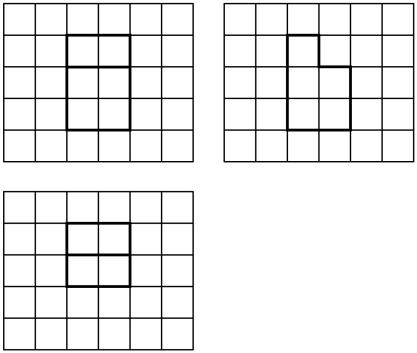
\includegraphics[width=.42\linewidth]{assets/asset-160-01.jpg}
\end{center}
\begin{choices}
  \item $24$
  \item $26$
  \item $28$
  \item $30$
\end{choices}
\begin{solution}
\textbf{答案：}$30$

\textbf{分析：}由题意首先由三视图还原空间几何体，然后由所得的空间几何体的结构特征求解其表面积即可.

\textbf{详解：}如图所示，在长方体 $ABCD-A_1B_1C_1D_1$中，$AB=BC=2$，$AA_1=3$，点 $H,I,J,K$ 为所在棱上靠近点 $B_1,C_1,D_1,A_1$ 的三等分点，$O,L,M,N$ 为所在棱的中点，则三视图所对应的几何体为长方体 $ABCD-A_1B_1C_1D_1$ 去掉长方体 $ONIC_1-LMHB_1$ 之后所得的几何体，该几何体的表面积和原来的长方体的表面积相比少2个边长为1的正方形，其表面积为：$2\times (2\times 2)+4\times (2\times 3)-2\times (1\times 1)=30$.
\end{solution}
\end{question}

\begin{question}[points=5]
\textbf{来源：}2023 年 全国乙卷-理科，第 8 题\par
已知圆锥 $PO$ 的底面半径为 $\sqrt{3}$，$O$ 为底面圆心，$PA$，$PB$ 为圆锥的母线，$\angle AOB=120^\circ$，若 $\triangle PAB$ 的面积等于 $\frac{9\sqrt{3}}{4}$，则该圆锥的体积为（ ）
\begin{choices}
  \item $\pi$
  \item $\sqrt{6}\pi$
  \item $3\pi$
  \item $3\sqrt{6}\pi$
\end{choices}
\begin{solution}
\textbf{答案：}$\sqrt{6}\pi$

\textbf{分析：}根据给定条件，利用三角形面积公式求出圆锥的母线长，进而求出圆锥的高，求出体积作答.

\textbf{详解：}在 $\triangle AOB$ 中，$\angle AOB=120^\circ$，而 $OA=OB=\sqrt{3}$，取 $AC$ 中点 $C$，连接 $OC,PC$，有 $OC\perp AB,PC\perp AB$，$\angle ABO=30^\circ$，$OC=\frac{\sqrt{3}}{2}$，$AB=2BC=3$，由 $\triangle PAB$ 的面积为 $\frac{9\sqrt{3}}{4}$，得 $\frac{1}{2}\times 3\times PC=\frac{9\sqrt{3}}{4}$，解得 $PC=\frac{3\sqrt{3}}{2}$，于是 $PO=\sqrt{PC^2-OC^2}=\sqrt{(\frac{3\sqrt{3}}{2})^2-(\frac{\sqrt{3}}{2})^2}=\sqrt{6}$，所以圆锥的体积 $V=\frac{1}{3}\pi\times OA^2\times PO=\frac{1}{3}\pi\times (\sqrt{3})^2\times \sqrt{6}=\sqrt{6}\pi$.
\end{solution}
\end{question}

\begin{question}[points=5]
\textbf{来源：}2023 年 全国乙卷-理科，第 9 题\par
已知 $\triangle ABC$ 为等腰直角三角形，$AB$ 为斜边，$\triangle ABD$ 为等边三角形，若二面角 $C-AB-D$ 为 $150^\circ$，则直线 $CD$ 与平面 $ABC$ 所成角的正切值为（ ）
\begin{choices}
  \item $\frac{1}{5}$
  \item $\frac{2}{5}$
  \item $\frac{\sqrt{3}}{5}$
  \item $\frac{2}{5}$
\end{choices}
\begin{solution}
\textbf{答案：}$\frac{\sqrt{3}}{5}$

\textbf{分析：}根据给定条件，推导确定线面角，再利用余弦定理、正弦定理求解作答.

\textbf{详解：}取 $AB$ 的中点 $E$，连接 $CE,DE$，因为 $\triangle ABC$ 是等腰直角三角形，且 $AB$ 为斜边，则有 $CE\perp AB$，又 $\triangle ABD$ 是等边三角形，则 $DE\perp AB$，从而 $\angle CED$ 为二面角 $C-AB-D$ 的平面角，即 $\angle CED=150^\circ$，显然 $CE\cap DE=E$，$CE,DE\subset$ 平面 $CDE$，于是 $AB\perp$ 平面 $CDE$，又 $AB\subset$ 平面 $ABC$，因此平面 $CDE\perp$ 平面 $ABC$，显然平面 $CDE\cap$ 平面 $ABC=CE$，直线 $CD\subset$ 平面 $CDE$，则直线 $CD$ 在平面 $ABC$ 内的射影为直线 $CE$，从而 $\angle DCE$ 为直线 $CD$ 与平面 $ABC$ 所成的角，令 $AB=2$，则 $CE=1$，$DE=\sqrt{3}$，在 $\triangle CDE$ 中，由余弦定理得：$CD=\sqrt{CE^2+DE^2-2CE\cdot DE\cos\angle CED}=\sqrt{1+3-2\times1\times\sqrt{3}\times(-\frac{\sqrt{3}}{2})}=\sqrt{7}$，由正弦定理得 $\frac{DE}{\sin\angle DCE}=\frac{CD}{\sin\angle CED}$，即 $\sin\angle DCE=\frac{\sqrt{3}\sin150^\circ}{\sqrt{7}}=\frac{\sqrt{3}}{2\sqrt{7}}$，显然 $\angle DCE$ 是锐角，$\cos\angle DCE=\sqrt{1-\sin^2\angle DCE}=\sqrt{1-(\frac{\sqrt{3}}{2\sqrt{7}})^2}=\frac{5}{2\sqrt{7}}$，所以直线 $CD$ 与平面 $ABC$ 所成的角的正切为 $\frac{\sqrt{3}}{5}$.
\end{solution}
\end{question}

\begin{question}[points=12]
\textbf{来源：}2023 年 全国乙卷-理科，第 19 题\par
如图，在三棱锥 $P-ABC$ 中，$AB\perp BC$，$AB=2$，$BC=2\sqrt{2}$，$PB=PC=\sqrt{6}$，$BP$，$AP$，$BC$ 的中点分别为 $D$，$E$，$O$，$AD=\sqrt{5}DO$，点 $F$ 在 $AC$ 上，$BF\perp AO$.



(1) 证明：$EF\parallel$ 平面 $ADO$；



(2) 证明：平面 $ADO\perp$ 平面 $BEF$；



(3) 求二面角 $D-AO-C$ 的正弦值.

\begin{center}
  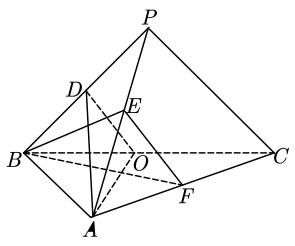
\includegraphics[width=.42\linewidth]{assets/asset-163-01.jpg}
\end{center}
\begin{solution}

\textbf{详解：}(1) 连接 $DE,OF$，设 $\overrightarrow{AF}=t\overrightarrow{AC}$，则 $\overrightarrow{BF}=\overrightarrow{BA}+\overrightarrow{AF}=(1-t)\overrightarrow{BA}+t\overrightarrow{BC}$，$\overrightarrow{AO}=-\overrightarrow{BA}+\frac{1}{2}\overrightarrow{BC}$，$BF\perp AO$，则 $\overrightarrow{BF}\cdot\overrightarrow{AO}=[(1-t)\overrightarrow{BA}+t\overrightarrow{BC}]\cdot(-\overrightarrow{BA}+\frac{1}{2}\overrightarrow{BC})=(t-1)BA^2+\frac{1}{2}tBC^2=4(t-1)+4t=0$，解得 $t=\frac{1}{2}$，则 $F$ 为 $AC$ 的中点，由 $D,E,O,F$ 分别为 $PB,PA,BC,AC$ 的中点，于是 $DE\parallel AB$，$DE=\frac{1}{2}AB$，$OF\parallel AB$，$OF=\frac{1}{2}AB$，即 $DE\parallel OF$，$DE=OF$，则四边形 $ODEF$ 为平行四边形，$EF\parallel DO$，$EF=DO$，又 $EF\not\subset$ 平面 $ADO$，$DO\subset$ 平面 $ADO$，所以 $EF\parallel$ 平面 $ADO$.

(2) 由(1)可知 $EF\parallel OD$，则 $AO=\sqrt{6}$，$DO=\frac{\sqrt{6}}{2}$，得 $AD=\sqrt{5}DO=\frac{\sqrt{30}}{2}$，因此 $OD^2+AO^2=AD^2=\frac{15}{2}$，则 $OD\perp AO$，有 $EF\perp AO$，又 $AO\perp BF$，$BF\cap EF=F$，$BF,EF\subset$ 平面 $BEF$，则有 $AO\perp$ 平面 $BEF$，又 $AO\subset$ 平面 $ADO$，所以平面 $ADO\perp$ 平面 $BEF$.

(3) 过点 $O$ 作 $OH\parallel BF$ 交 $AC$ 于点 $H$，设 $AD\cap BE=G$，由 $AO\perp BF$，得 $HO\perp AO$，且 $FH=\frac{1}{3}AH$，又由(2)知，$OD\perp AO$，则 $\angle DOH$ 为二面角 $D-AO-C$ 的平面角，因为 $D,E$ 分别为 $PB,PA$ 的中点，因此 $G$ 为 $\triangle PAB$ 的重心，即有 $DG=\frac{1}{3}AD$，$GE=\frac{1}{3}BE$，又 $FH=\frac{1}{3}AH$，即有 $DH=GF$，$\cos\angle ABD=\frac{4+\frac{3}{2}-\frac{PA^2}{2}}{2\times2\times\frac{\sqrt{6}}{2}}=\frac{4+6-PA^2}{2\times2\times\sqrt{6}}$，解得 $PA=\sqrt{14}$，同理得 $BE=\frac{\sqrt{6}}{2}$，于是 $BE^2+EF^2=BF^2=3$，即有 $BE\perp EF$，则 $GF=\sqrt{(\frac{1}{3}\times\frac{\sqrt{6}}{2})^2+(\frac{\sqrt{6}}{2})^2}=\frac{\sqrt{15}}{3}$，从而 $GF=\frac{\sqrt{15}}{3}$，$DH=\frac{3}{2}\times\frac{\sqrt{15}}{3}=\frac{\sqrt{15}}{2}$，在 $\triangle DOH$ 中，$OH=\frac{1}{2}BF=\frac{\sqrt{3}}{2}$，$OD=\frac{\sqrt{6}}{2}$，$DH=\frac{\sqrt{15}}{2}$，于是 $\cos\angle DOH=\frac{\frac{6}{4}+\frac{3}{4}-\frac{15}{4}}{2\times\frac{\sqrt{6}}{2}\times\frac{\sqrt{3}}{2}}=-\frac{\sqrt{2}}{2}$，$\sin\angle DOH=\sqrt{1-(-\frac{\sqrt{2}}{2})^2}=\frac{\sqrt{2}}{2}$，所以二面角 $D-AO-C$ 的正弦值为 $\frac{\sqrt{2}}{2}$.
\end{solution}
\end{question}

\begin{question}[points=5]
\textbf{来源：}2023 年 全国乙卷-文科，第 3 题\par
如图，网格纸上绘制的一个零件的三视图，网格小正方形的边长为1，则该零件的表面积为（   ）

\begin{center}
  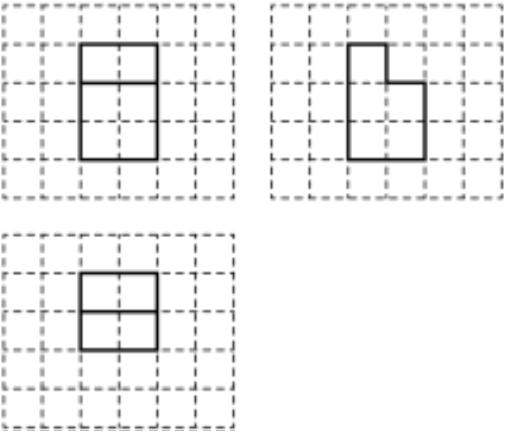
\includegraphics[width=.42\linewidth]{assets/asset-164-01.jpg}
\end{center}
\begin{choices}
  \item $24$
  \item $26$
  \item $28$
  \item $30$
\end{choices}
\begin{solution}
\textbf{答案：}$30$

\textbf{分析：}由题意首先由三视图还原空间几何体，然后由所得的空间几何体的结构特征求解其表面积即可.

\textbf{详解：}如图所示，在长方体$ABCD-A_1B_1C_1D_1$中，$AB=BC=2$，$AA_1=3$，点$H,I,J,K$为所在棱上靠近点$B_1,C_1,D_1,A_1$的三等分点，$O,L,M,N$为所在棱的中点，则三视图所对应的几何体为长方体$ABCD-A_1B_1C_1D_1$去掉长方体$ONIC_1-LMHB_1$之后所得的几何体，该几何体的表面积和原来的长方体的表面积相比少2个边长为1的正方形，其表面积为：$2\times(2\times2)+4\times(2\times3)-2\times(1\times1)=30$. 故选D.
\end{solution}
\end{question}

\begin{question}[points=5]
\textbf{来源：}2023 年 全国乙卷-文科，第 16 题\par
已知点$S,A,B,C$均在半径为2的球面上，$\triangle ABC$是边长为3的等边三角形，$SA\perp$平面$ABC$，则$SA=$.
\fillin[{$2$}]
\begin{solution}
\textbf{答案：}$2$

\textbf{分析：}先用正弦定理求底面外接圆半径，再结合直棱柱的外接球以及球的性质运算求解.

\textbf{详解：}如图，将三棱锥$S-ABC$转化为直三棱柱$SMN-ABC$，设$\triangle ABC$的外接圆圆心为$O_1$，半径为$r$，则$2r=\frac{AB}{\sin\angle ACB}=\frac{3}{\frac{\sqrt{3}}{2}}=2\sqrt{3}$，可得$r=\sqrt{3}$，设三棱锥$S-ABC$的外接球球心为$O$，连接$OA, OO_1$，则$OA=2, OO_1=\frac{1}{2}SA$，因为$OA^2=OO_1^2+O_1A^2$，即$4=3+\frac{1}{4}SA^2$，解得$SA=2$. 故答案为2.
\end{solution}
\end{question}

\begin{question}[points=12]
\textbf{来源：}2023 年 全国乙卷-文科，第 19 题\par
如图，在三棱锥$P-ABC$中，$AB\perp BC$，$AB=2$，$BC=2\sqrt{2}$，$PB=PC=\sqrt{6}$，$BP, AP, BC$的中点分别为$D, E, O$，点$F$在$AC$上，$BF\perp AO$．

（1）求证：$EF\parallel$平面$ADO$；

（2）若$\angle POF=120^\circ$，求三棱锥$P-ABC$的体积．
\begin{solution}

\textbf{分析：}（1）根据给定条件，证明四边形$ODEF$为平行四边形，再利用线面平行的判定推理作答.
（2）作出并证明$PM$为棱锥的高，利用三棱锥的体积公式直接可求体积.

\textbf{详解：}（1）连接$DE, OF$，设$\overrightarrow{AF}=t\overrightarrow{AC}$，则$\overrightarrow{BF}=\overrightarrow{BA}+\overrightarrow{AF}=(1-t)\overrightarrow{BA}+t\overrightarrow{BC}$，$\overrightarrow{AO}=-\overrightarrow{BA}+\frac{1}{2}\overrightarrow{BC}$，$\overrightarrow{BF}\perp\overrightarrow{AO}$，则$\overrightarrow{BF}\cdot\overrightarrow{AO}=[(1-t)\overrightarrow{BA}+t\overrightarrow{BC}]\cdot(-\overrightarrow{BA}+\frac{1}{2}\overrightarrow{BC})=(t-1)|\overrightarrow{BA}|^2+\frac{t}{2}|\overrightarrow{BC}|^2=4(t-1)+4t=0$，解得$t=\frac{1}{2}$，则$F$为$AC$的中点，由$D,E,O,F$分别为$PB,PA,BC,AC$的中点，于是$DE\parallel AB, DE=\frac{1}{2}AB, OF\parallel AB, OF=\frac{1}{2}AB$，即$DE\parallel OF, DE=OF$，则四边形$ODEF$为平行四边形，$EF\parallel DO, EF=DO$，又$EF\not\subset$平面$ADO, DO\subset$平面$ADO$，所以$EF\parallel$平面$ADO$.
（2）过$P$作$PM$垂直$FO$的延长线交于点$M$，因为$PB=PC, O$是$BC$中点，所以$PO\perp BC$，在$\mathrm{Rt}\triangle PBO$中，$PB=\sqrt{6}, BO=\frac{1}{2}BC=\sqrt{2}$，所以$PO=\sqrt{PB^2-OB^2}=\sqrt{6-2}=2$，因为$AB\perp BC, OF\parallel AB$，所以$OF\perp BC$，又$PO\cap OF=O, PO,OF\subset$平面$POF$，所以$BC\perp$平面$POF$，又$PM\subset$平面$POF$，所以$BC\perp PM$，又$BC\parallel FM=O, BC,FM\subset$平面$ABC$，所以$PM\perp$平面$ABC$，即三棱锥$P-ABC$的高为$PM$，因为$\angle POF=120^\circ$，所以$\angle POM=60^\circ$，所以$PM=PO\sin60^\circ=2\times\frac{\sqrt{3}}{2}=\sqrt{3}$，又$S_{\triangle ABC}=\frac{1}{2}AB\cdot BC=\frac{1}{2}\times2\times2\sqrt{2}=2\sqrt{2}$，所以$V_{P-ABC}=\frac{1}{3}S_{\triangle ABC}\cdot PM=\frac{1}{3}\times2\sqrt{2}\times\sqrt{3}=\frac{2\sqrt{6}}{3}$.
\end{solution}
\end{question}

\begin{question}[points=5]
\textbf{来源：}2023 年 上海卷，第 12 题；次专题：计数原理\par
空间内存在三点 $A,B,C$，满足 $AB=AC=BC=2$，在空间内取不同两点(不计顺序),使得这两点与 $A,B,C$ 可以组成正四棱锥,求方案数为
\fillin[{$9$}]
\begin{solution}
\textbf{答案：}$9$
\end{solution}
\end{question}

\begin{question}[points=14]
\textbf{来源：}2023 年 上海卷，第 17 题\par
直四棱柱 $ABCD-A_1B_1C_1D_1$，$AB\parallel CD$，$AB=2$，$CD=4$，$AD=1$，$\angle BAD=90^\circ$。

(1)求证：$A_1B\parallel$ 平面 $DCC_1D_1$；

(2)若四棱柱体积为 $36$，求二面角 $A_1-BD-C$ 的大小。

\begin{center}
  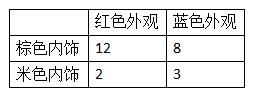
\includegraphics[width=.42\linewidth]{assets/asset-168-01.jpg}
\end{center}
\begin{solution}

\textbf{详解：}(1) 因为 $AB\parallel CD$，所以 $AB\parallel$ 平面 $DCC_1D_1$。又因为 $AA_1\parallel DD_1$，所以 $AA_1\parallel$ 平面 $DCC_1D_1$。因为 $AA_1$ 与 $AB$ 相交于点 $A$，所以平面 $AA_1B\parallel$ 平面 $DCC_1D_1$。因为 $A_1B\subset$ 平面 $AA_1B$，所以 $A_1B\parallel$ 平面 $DCC_1D_1$。
(2) 设 $AA_1=h$，四棱柱体积 $V=S_{ABCD}\cdot h$。$S_{ABCD}=\frac{1}{2}(AB+CD)\cdot AD=\frac{1}{2}(2+4)\times 1=3$，则 $3h=36$，得 $h=12$。在底面内作 $AE\perp BD$ 于 $E$，连接 $A_1E$。因为 $BD\perp AE$，$BD\perp AA_1$，所以 $BD\perp$ 平面 $AA_1E$，所以 $BD\perp A_1E$。故 $\angle A_1EA$ 即为所求二面角的平面角。在 $\triangle ABD$ 中，$AB=2$，$AD=1$，$\angle BAD=90^\circ$，则 $BD=\sqrt{5}$，$AE=\frac{AB\cdot AD}{BD}=\frac{2\times1}{\sqrt{5}}=\frac{2}{\sqrt{5}}$。在 $\triangle A_1AE$ 中，$AA_1=12$，则 $\tan\angle A_1EA=\frac{AA_1}{AE}=12\times\frac{\sqrt{5}}{2}=6\sqrt{5}$。所以 $\angle A_1EA=\arctan(6\sqrt{5})$。
\end{solution}
\end{question}

\begin{question}[points=5]
\textbf{来源：}2023 年 天津卷，第 8 题\par
在三棱锥 $P-ABC$ 中, 线段 $PC$ 上的点 $M$ 满足 $PM = \dfrac{1}{3}PC$, 线段 $PB$ 上的点 $N$ 满足 $PN = \dfrac{2}{3}PB$, 则三棱锥 $P-AMN$ 和三棱锥 $P-ABC$ 的体积之比为 ( )
\begin{choices}
  \item $\dfrac{1}{9}$
  \item $\dfrac{2}{9}$
  \item $\dfrac{1}{3}$
  \item $\dfrac{4}{9}$
\end{choices}
\begin{solution}
\textbf{答案：}B

\textbf{分析：}分别过 M, C 作 $MM' \perp PA$, $CC' \perp PA$, 过 B 作 $BB' \perp$ 平面 $PAC$, 连接 $PB'$, 过 N 作 $NN' \perp PB'$. 利用相似比和体积公式.

\textbf{详解：}如图, 分别过 $M, C$ 作 $MM' \perp PA$, $CC' \perp PA$, 垂足分别为 $M', C'$. 过 $B$ 作 $BB' \perp$ 平面 $PAC$, 垂足为 $B'$, 连接 $PB'$, 过 $N$ 作 $NN' \perp PB'$, 垂足为 $N'$. 因为 $BB' \perp$ 平面 $PAC$, $BB' \subset$ 平面 $PBB'$, 所以平面 $PBB' \perp$ 平面 $PAC$. 又因为平面 $PBB' \cap$ 平面 $PAC = PB'$, $NN' \perp PB'$, $NN' \subset$ 平面 $PBB'$, 所以 $NN' \perp$ 平面 $PAC$, 且 $BB' \parallel NN'$. 在 $\triangle PCC'$ 中, 因为 $MM' \perp PA$, $CC' \perp PA$, 所以 $MM' \parallel CC'$, 所以 $\dfrac{PM}{PC} = \dfrac{MM'}{CC'} = \dfrac{1}{3}$. 在 $\triangle PBB'$ 中, 因为 $BB' \parallel NN'$, 所以 $\dfrac{PN}{PB} = \dfrac{NN'}{BB'} = \dfrac{2}{3}$. 所以 $\dfrac{V_{P-AMN}}{V_{P-ABC}} = \dfrac{V_{N-PAM}}{V_{B-PAC}} = \dfrac{\frac{1}{3} S_{\triangle PAM} \cdot NN'}{\frac{1}{3} S_{\triangle PAC} \cdot BB'} = \dfrac{\frac{1}{2} PA \cdot MM' \cdot NN'}{\frac{1}{2} PA \cdot CC' \cdot BB'} = \dfrac{1}{3} \cdot \frac{2}{3} = \dfrac{2}{9}$.
\end{solution}
\end{question}

\begin{question}[points=15]
\textbf{来源：}2023 年 天津卷，第 17 题\par
三棱台 $ABC-A_1B_1C_1$ 中，若 $A_1A \perp$ 面 $ABC$, $AB \perp AC$, $AB = AC = AA_1 = 2$, $A_1C_1 = 1$, $M, N$ 分别是 $BC, BA$ 中点.

(1) 求证：$A_1N \parallel$ 平面 $C_1MA$;

(2) 求平面 $C_1MA$ 与平面 $ACC_1A_1$ 所成夹角的余弦值;

(3) 求点 $C$ 到平面 $C_1MA$ 的距离.

\begin{center}
  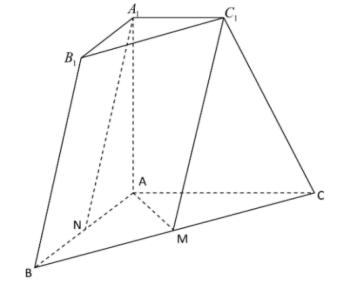
\includegraphics[width=.42\linewidth]{assets/asset-170-01.jpg}
\end{center}
\begin{solution}
\textbf{答案：}(1) 证明见解析; (2) $\dfrac{2}{3}$; (3) $\dfrac{4}{3}$

\textbf{详解：}(1) 连接 $MN$, $C_1A$. 由 $M,N$ 分别是 $BC,BA$ 中点, 得 $MN \parallel AC$ 且 $MN = \frac{AC}{2}=1$. 由棱台性质, $A_1C_1 \parallel AC$, 所以 $MN \parallel A_1C_1$, 且 $MN = A_1C_1 = 1$, 故四边形 $MNA_1C_1$ 是平行四边形, 所以 $A_1N \parallel MC_1$. 又 $A_1N \not\subset$ 平面 $C_1MA$, $MC_1 \subset$ 平面 $C_1MA$, 所以 $A_1N \parallel$ 平面 $C_1MA$.
(2) 过 $M$ 作 $ME \perp AC$ 于 $E$, 过 $E$ 作 $EF \perp AC_1$ 于 $F$, 连接 $MF$. 由 $A_1A \perp$ 面 $ABC$, $ME \subset$ 面 $ABC$, 得 $AA_1 \perp ME$, 又 $ME \perp AC$, $AC \cap AA_1 = A$, 所以 $ME \perp$ 平面 $ACC_1A_1$. 故 $ME \perp AC_1$. 又 $EF \perp AC_1$, 所以 $AC_1 \perp$ 平面 $MEF$, 则 $AC_1 \perp MF$. 故 $\angle MFE$ 为平面 $C_1MA$ 与平面 $ACC_1A_1$ 所成角. 计算得 $ME = \frac{AB}{2}=1$, $\cos\angle CAC_1 = \frac{1}{\sqrt{5}}$, $\sin\angle CAC_1 = \frac{2}{\sqrt{5}}$, $EF = 1 \cdot \sin\angle CAC_1 = \frac{2}{\sqrt{5}}$, $MF = \sqrt{ME^2 + EF^2} = \sqrt{1 + \frac{4}{5}} = \frac{3}{\sqrt{5}}$, 所以 $\cos\angle MFE = \frac{EF}{MF} = \frac{2}{3}$.
(3) [方法一] 过 $C_1$ 作 $C_1P \perp AC$ 于 $P$, 作 $C_1Q \perp AM$ 于 $Q$, 连接 $PQ, PM$, 过 $P$ 作 $PR \perp C_1Q$ 于 $R$. 计算得 $C_1A = C_1C = \sqrt{5}$, $C_1M = \sqrt{5}$, $C_1Q = \frac{3\sqrt{2}}{2}$, $PR = \frac{PC_1 \cdot PQ}{QC_1} = \frac{2 \cdot \frac{\sqrt{2}}{2}}{\frac{3\sqrt{2}}{2}} = \frac{2}{3}$. 因为 $CA = 2PA$, 所以点 $C$ 到平面 $C_1MA$ 的距离是点 $P$ 到该平面距离的两倍, 即 $\frac{4}{3}$.
[方法二] 设点 $C$ 到平面 $C_1MA$ 的距离为 $h$. $V_{C_1-AMC} = \frac{1}{3} \cdot C_1P \cdot S_{\triangle AMC} = \frac{1}{3} \cdot 2 \cdot \frac{1}{2} \cdot 2 \cdot 2 = \frac{4}{3}$. 又 $V_{C-C_1MA} = \frac{1}{3} \cdot h \cdot S_{\triangle AMC_1} = \frac{1}{3} \cdot h \cdot \frac{1}{2} \cdot 2 \cdot \frac{3\sqrt{2}}{2} = \frac{h}{2}$. 由 $V_{C_1-AMC} = V_{C-C_1MA}$ 得 $\frac{h}{2} = \frac{4}{3}$, 所以 $h = \frac{4}{3}$.
\end{solution}
\end{question}

\begin{question}[points=5]
\textbf{来源：}2023 年 新高考II卷，第 9 题\par
已知圆锥的顶点为$P$，底面圆心为$O$，$AB$为底面直径，$\angle APB=120^{\circ}$，$PA=2$，点$C$在底面圆周上，且二面角$P-AC-O$为$45^{\circ}$，则（ \quad ）
\begin{choices}
  \item A. 该圆锥的体积为$\pi$
  \item B. 该圆锥的侧面积为$4\sqrt{3}\pi$
  \item C. $AC=2\sqrt{2}$
  \item D. $\triangle PAC$的面积为$\sqrt{3}$
\end{choices}
\begin{solution}
\textbf{答案：}AC

\textbf{分析：}根据圆锥的体积、侧面积判断A、B选项的正确性，利用二面角的知识判断C、D选项的正确性.

\textbf{详解：}依题意，$\angle APB=120^{\circ}$，$PA=2$，所以$OP=1$，$OA=OB=\sqrt{3}$；A选项，圆锥的体积为$\dfrac{1}{3}\times\pi\times(\sqrt{3})^{2}\times1=\pi$，A正确；B选项，圆锥的侧面积为$\pi\times\sqrt{3}\times2=2\sqrt{3}\pi$，B错误；C选项，设$D$是$AC$的中点，连接$OD,PD$，则$AC\perp OD$，$AC\perp PD$，所以$\angle PDO$是二面角$P-AC-O$的平面角，则$\angle PDO=45^{\circ}$，所以$OP=OD=1$，故$AD=CD=\sqrt{3-1}=\sqrt{2}$，则$AC=2\sqrt{2}$，C正确；D选项，$PD=\sqrt{1^{2}+1^{2}}=\sqrt{2}$，所以$S_{\triangle PAC}=\dfrac{1}{2}\times2\sqrt{2}\times\sqrt{2}=2$，D错误.
\end{solution}
\end{question}

\begin{question}[points=5]
\textbf{来源：}2023 年 新高考II卷，第 14 题\par
底面边长为4的正四棱锥被平行于其底面的平面所截，截去一个底面边长为2，高为3的正四棱锥，所得棱台的体积为．
\fillin[{$28$}]
\begin{solution}
\textbf{答案：}$28$

\textbf{分析：}方法一：割补法，根据正四棱锥的几何性质以及棱锥体积公式求得正确答案；方法二：根据台体的体积公式直接运算求解.

\textbf{详解：}方法一：由于$\dfrac{2}{4}=\dfrac{1}{2}$，而截去的正四棱锥的高为3，所以原正四棱锥的高为6，所以原正四棱锥的体积为$\dfrac{1}{3}\times(4\times4)\times6=32$，截去的正四棱锥的体积为$\dfrac{1}{3}\times(2\times2)\times3=4$，所以棱台的体积为$32-4=28$.
方法二：棱台的体积为$\dfrac{1}{3}\times3\times(16+4+\sqrt{16\times4})=28$.
\end{solution}
\end{question}

\begin{question}[points=10]
\textbf{来源：}2023 年 新高考II卷，第 20 题\par
如图，三棱锥$A-BCD$中，$DA=DB=DC$，$BD\perp CD$，$\angle ADB=\angle ADC=60^{\circ}$，$E$为$BC$的中点．

（1）证明：$BC\perp DA$；

（2）点$F$满足$\overrightarrow{EF}=\overrightarrow{DA}$，求二面角$D-AB-F$的正弦值．

\begin{center}
  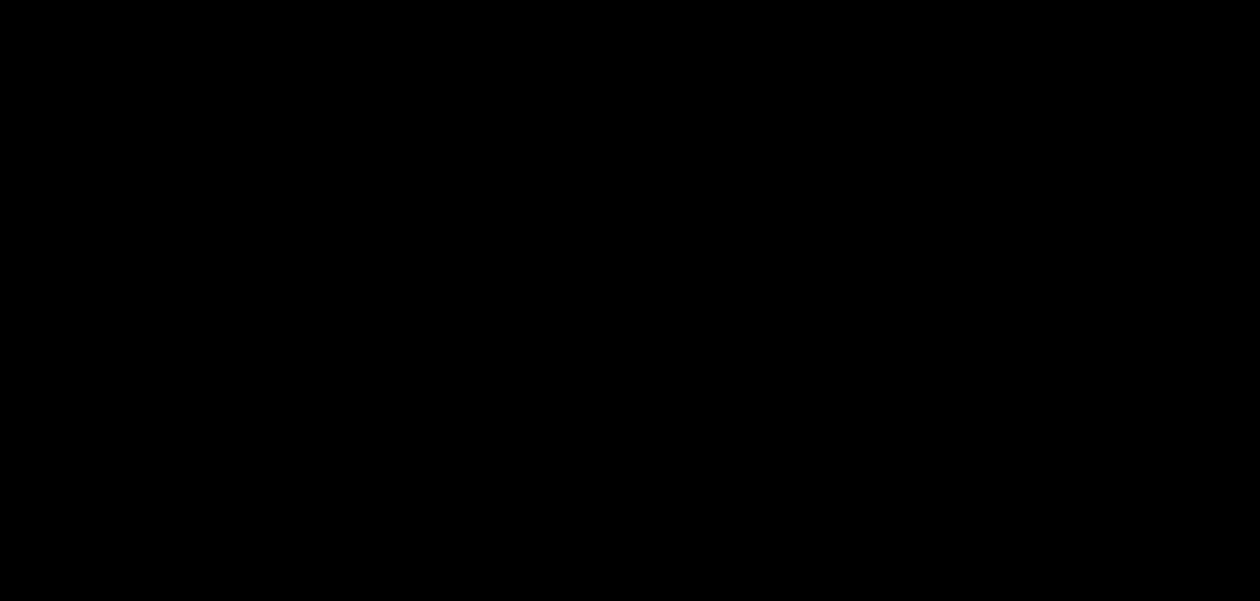
\includegraphics[width=.42\linewidth]{assets/asset-173-01.jpg}
\end{center}
\begin{solution}
\textbf{答案：}（1）证明见解析；（2）$\dfrac{\sqrt{3}}{3}$.

\textbf{分析：}（1）根据题意易证$BC\perp$平面$ADE$，从而证得$BC\perp DA$；
（2）由题可证$AE\perp$平面$BCD$，所以以点$E$为原点，$ED,EB,EA$所在直线分别为$x,y,z$轴，建立空间直角坐标系，再求出平面$ABD$，$ABF$的一个法向量，根据二面角的向量公式以及同角三角函数关系即可解出.

\textbf{详解：}（1）连接$AE,DE$，因为$E$为$BC$中点，$DB=DC$，所以$DE\perp BC$①，因为$DA=DB=DC$，$\angle ADB=\angle ADC=60^{\circ}$，所以$\triangle ACD$与$\triangle ABD$均为等边三角形，$\therefore AC=AB$，从而$AE\perp BC$②，由①②，$AE\cap DE=E$，$AE,DE\subset$平面$ADE$，所以$BC\perp$平面$ADE$，而$AD\subset$平面$ADE$，所以$BC\perp DA$.
（2）不妨设$DA=DB=DC=2$，$\because BD\perp CD$，$\therefore BC=2\sqrt{2}$，$DE=AE=\sqrt{2}$，$\because AE^{2}+DE^{2}=4=AD^{2}$，$\therefore AE\perp DE$，又$\because AE\perp BC$，$DE\cap BC=E$，$DE,BC\subset$平面$BCD$，$\therefore AE\perp$平面$BCD$．以点$E$为原点，$ED,EB,EA$所在直线分别为$x,y,z$轴，建立空间直角坐标系，如图所示：
设$D(\sqrt{2},0,0)$，$A(0,0,\sqrt{2})$，$B(0,\sqrt{2},0)$，$E(0,0,0)$，设平面$DAB$与平面$ABF$的一个法向量分别为$\vec{n_{1}}=(x_{1},y_{1},z_{1})$，$\vec{n_{2}}=(x_{2},y_{2},z_{2})$，二面角$D-AB-F$平面角为$\theta$，而$\overrightarrow{AB}=(0,\sqrt{2},-\sqrt{2})$，因为$\overrightarrow{EF}=\overrightarrow{DA}=(-\sqrt{2},0,\sqrt{2})$，所以$F(-\sqrt{2},0,\sqrt{2})$，即有$\overrightarrow{AF}=(-\sqrt{2},0,0)$，$\therefore\begin{cases}-\sqrt{2}x_{1}+\sqrt{2}z_{1}=0\\ \sqrt{2}y_{1}-\sqrt{2}z_{1}=0\end{cases}$，取$x_{1}=1$，所以$\vec{n_{1}}=(1,1,1)$；$\begin{cases}\sqrt{2}y_{2}-\sqrt{2}z_{2}=0\\ -\sqrt{2}x_{2}=0\end{cases}$，取$y_{2}=1$，所以$\vec{n_{2}}=(0,1,1)$，所以$\cos\theta=\dfrac{\vec{n_{1}}\cdot\vec{n_{2}}}{|\vec{n_{1}}||\vec{n_{2}}|}=\dfrac{2}{\sqrt{3}\times\sqrt{2}}=\dfrac{\sqrt{6}}{3}$，从而$\sin\theta=\sqrt{1-\dfrac{6}{9}}=\dfrac{\sqrt{3}}{3}$，所以二面角$D-AB-F$的正弦值为$\dfrac{\sqrt{3}}{3}$.
\end{solution}
\end{question}

\begin{question}[points=5]
\textbf{来源：}2023 年 新高考I卷，第 12 题\par
下列物体中，能够被整体放入棱长为 1（单位：m）的正方体容器（容器壁厚度忽略不计）内的有（ ）
\begin{choices}
  \item 直径为 0.99m 的球体
  \item 所有棱长均为 1.4m 的四面体
  \item 底面直径为 0.01m，高为 1.8m 的圆柱体
  \item 底面直径为 1.2m，高为 0.01m 的圆柱体
\end{choices}
\begin{solution}
\textbf{答案：}ABD

\textbf{分析：}根据题意结合正方体的性质逐项分析判断。

\textbf{详解：}对于选项 A：因为 $0.99\text{m}<1\text{m}$，即球体的直径小于正方体的棱长，所以能够被整体放入正方体内，故 A 正确。对于选项 B：因为正方体的面对角线长为 $\sqrt{2}\text{m}$，且 $\sqrt{2}>1.4$，所以能够被整体放入正方体内，故 B 正确。对于选项 C：因为正方体的体对角线长为 $\sqrt{3}\text{m}$，且 $\sqrt{3}<1.8$，所以不能够被整体放入正方体内，故 C 错误。对于选项 D：因为正方体的体对角线长为 $\sqrt{3}\text{m}$，且 $\sqrt{3}>1.2$，设正方体 $ABCD-A_1B_1C_1D_1$ 的中心为 $O$，以 $AC_1$ 为轴对称放置圆柱，设圆柱的底面圆心 $O_1$ 到正方体的表面的最近的距离为 $h\text{m}$，如图，结合对称性可知：$OC_1=\frac{1}{2}C_1A=\frac{\sqrt{3}}{2}, C_1O_1=OC_1-OO_1=\frac{\sqrt{3}}{2}-0.6$，则 $\frac{h}{AA_1}=\frac{C_1O_1}{C_1A}$，即 $\frac{h}{1}=\frac{\frac{\sqrt{3}}{2}-0.6}{\sqrt{3}}$，解得 $h=\frac{1}{2}-\frac{0.6}{\sqrt{3}}>0.34>0.01$，所以能够被整体放入正方体内，故 D 正确。
\end{solution}
\end{question}

\begin{question}[points=5]
\textbf{来源：}2023 年 新高考I卷，第 14 题\par
在正四棱台 $ABCD-A_1B_1C_1D_1$ 中，$AB=2, A_1B_1=1, AA_1=\sqrt{2}$，则该棱台的体积为．

\begin{center}
  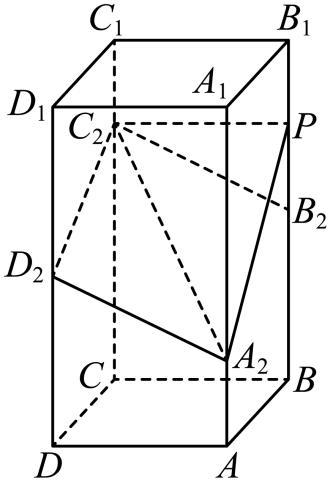
\includegraphics[width=.42\linewidth]{assets/asset-175-01.jpg}
\end{center}
\fillin[{$\frac{7\sqrt{6}}{6}$}]
\begin{solution}
\textbf{答案：}$\frac{7\sqrt{6}}{6}$

\textbf{分析：}结合图像，依次求得 $A_1O_1, AO, A_1M$，从而利用棱台的体积公式即可得解。

\textbf{详解：}如图，过 $A_1$ 作 $A_1M\perp AC$，垂足为 $M$，易知 $A_1M$ 为四棱台 $ABCD-A_1B_1C_1D_1$ 的高，因为 $AB=2, A_1B_1=1, AA_1=\sqrt{2}$，则 $A_1O_1=\frac{1}{2}A_1C_1=\frac{1}{2}\times\sqrt{2}A_1B_1=\frac{\sqrt{2}}{2}, AO=\frac{1}{2}AC=\frac{1}{2}\times\sqrt{2}AB=\sqrt{2}$，故 $AM=\frac{1}{2}(AC-A_1C_1)=\frac{\sqrt{2}}{2}$，则 $A_1M=\sqrt{A_1A^2-AM^2}=\sqrt{2-\frac{1}{2}}=\frac{\sqrt{6}}{2}$，所以所求体积为 $V=\frac{1}{3}\times(4+1+\sqrt{4\times1})\times\frac{\sqrt{6}}{2}=\frac{7\sqrt{6}}{6}$。
\end{solution}
\end{question}

\begin{question}[points=12]
\textbf{来源：}2023 年 新高考I卷，第 18 题\par
如图，在正四棱柱 $ABCD-A_1B_1C_1D_1$ 中，$AB=2, AA_1=4$．点 $A_2, B_2, C_2, D_2$ 分别在棱 $AA_1, BB_1, CC_1, DD_1$ 上，$AA_2=1, BB_2=DD_2=2, CC_2=3$．



（1）证明：$B_2C_2\parallel A_2D_2$；

（2）点 $P$ 在棱 $BB_1$ 上，当二面角 $P-A_2C_2-D_2$ 为 $150^\circ$ 时，求 $B_2P$．
\begin{solution}
\textbf{答案：}（1）证明见解析；（2）1

\textbf{分析：}（1）建立空间直角坐标系，利用向量坐标相等证明；（2）设 $P(0,2,\lambda)(0\leq\lambda\leq4)$，利用向量法求二面角，建立方程求出 $\lambda$ 即可得解。

\textbf{详解：}（1）以 $C$ 为坐标原点，$CD, CB, CC_1$ 所在直线为 $x, y, z$ 轴建立空间直角坐标系，如图，则 $C(0,0,0), C_2(0,0,3), B_2(0,2,2), D_2(2,0,2), A_2(2,2,1)$，所以 $\overrightarrow{B_2C_2}=(0,-2,1), \overrightarrow{A_2D_2}=(0,-2,1)$，所以 $\overrightarrow{B_2C_2}\parallel\overrightarrow{A_2D_2}$，又 $B_2C_2, A_2D_2$ 不在同一条直线上，所以 $B_2C_2\parallel A_2D_2$。（2）设 $P(0,2,\lambda)(0\leq\lambda\leq4)$，则 $\overrightarrow{A_2C_2}=(-2,-2,2), \overrightarrow{PC_2}=(0,-2,3-\lambda), \overrightarrow{D_2C_2}=(-2,0,1)$，设平面 $PA_2C_2$ 的法向量 $\vec{n}=(x,y,z)$，则 $\begin{cases} \vec{n}\cdot\overrightarrow{A_2C_2}=-2x-2y+2z=0 \\ \vec{n}\cdot\overrightarrow{PC_2}=-2y+(3-\lambda)z=0 \end{cases}$，令 $z=2$，得 $y=3-\lambda, x=\lambda-1$，所以 $\vec{n}=(\lambda-1,3-\lambda,2)$，设平面 $A_2C_2D_2$ 的法向量 $\vec{m}=(a,b,c)$，则 $\begin{cases} \vec{m}\cdot\overrightarrow{A_2C_2}=-2a-2b+2c=0 \\ \vec{m}\cdot\overrightarrow{D_2C_2}=-2a+c=0 \end{cases}$，令 $a=1$，得 $b=1, c=2$，所以 $\vec{m}=(1,1,2)$，所以 $\cos\langle\vec{n},\vec{m}\rangle=\frac{\vec{n}\cdot\vec{m}}{|\vec{n}||\vec{m}|}=\frac{6}{\sqrt{6}\sqrt{4+(\lambda-1)^2+(3-\lambda)^2}}=\cos150^\circ=-\frac{\sqrt{3}}{2}$，化简可得 $\lambda^2-4\lambda+3=0$，解得 $\lambda=1$ 或 $\lambda=3$，所以 $P(0,2,1)$ 或 $P(0,2,3)$，所以 $B_2P=1$。
\end{solution}
\end{question}

\section*{2024 年}

\begin{question}[points=4]
\textbf{来源：}2024 年 北京卷，第 8 题\par
已知以边长为4的正方形为底面的四棱锥，四条侧棱分别为4，4，$2\sqrt{2}$，$2\sqrt{2}$，则该四棱锥的高为（ ）
\begin{choices}
  \item $\dfrac{\sqrt{2}}{2}$
  \item $\dfrac{\sqrt{3}}{2}$
  \item $2\sqrt{3}$
  \item $\sqrt{3}$
\end{choices}
\begin{solution}
\textbf{答案：}D

\textbf{分析：}取点作辅助线，根据题意分析可知平面 $PEF \perp$ 平面 $ABCD$，可知 $PO \perp$ 平面 $ABCD$，利用等体积法求点到面的距离。

\textbf{详解：}如图，底面 $ABCD$ 为正方形，当相邻的棱长相等时，不妨设 $PA=PB=AB=4, PC=PD=2\sqrt{2}$。分别取 $AB, CD$ 的中点 $E,F$，连接 $PE, PF, EF$，则 $PE \perp AB, EF \perp AB$，且 $PE \cap EF = E$，$PE, EF \subset$ 平面 $PEF$，可知 $AB \perp$ 平面 $PEF$，且 $AB \subset$ 平面 $ABCD$，所以平面 $PEF \perp$ 平面 $ABCD$。过 $P$ 作 $EF$ 的垂线，垂足为 $O$，即 $PO \perp EF$，由平面 $PEF \cap$ 平面 $ABCD = EF$，$PO \subset$ 平面 $PEF$，所以 $PO \perp$ 平面 $ABCD$。由题意可得：$PE=2\sqrt{3}, PF=2, EF=4$，则 $PE^2+PF^2=EF^2$，即 $PE \perp PF$，则 $\dfrac{1}{2} PE \cdot PF = \dfrac{1}{2} PO \cdot EF$，可得 $PO = \dfrac{PE \cdot PF}{EF} = \sqrt{3}$。所以四棱锥的高为 $\sqrt{3}$。当相对的棱长相等时，不妨设 $PA=PC=4, PB=PD=2\sqrt{2}$，因为 $BD=4\sqrt{2}=PB+PD$，此时不能形成三角形 $PBD$，与题意不符，这种情况不存在。故选：D。
\end{solution}
\end{question}

\begin{question}[points=15]
\textbf{来源：}2024 年 北京卷，第 17 题\par
已知四棱锥 $P-ABCD$，$AD\parallel BC$，$AB=BC=1$，$AD=3$，$DE=PE=2$，$E$ 是 $AD$ 上一点，$PE \perp AD$。

（1）若 $F$ 是 $PE$ 中点，证明：$BF\parallel$ 平面 $PCD$。

（2）若 $AB \perp$ 平面 $PED$，求平面 $PAB$ 与平面 $PCD$ 夹角的余弦值。

\begin{center}
  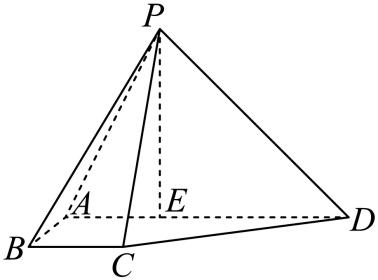
\includegraphics[width=.42\linewidth]{assets/asset-178-01.jpg}
\end{center}
\begin{solution}
\textbf{答案：}（1）证明见解析；（2）$\dfrac{\sqrt{30}}{30}$

\textbf{分析：}（1）取 $PD$ 的中点为 $S$，连接 $SF, SC$，可证四边形 $SFBC$ 为平行四边形，由线面平行的判定定理可得 $BF\parallel$ 平面 $PCD$。
（2）建立如图所示的空间直角坐标系，求出平面 $APB$ 和平面 $PCD$ 的法向量后可求夹角的余弦值。

\textbf{详解：}（1）取 $PD$ 的中点为 $S$，连接 $SF, SC$，则 $SF\parallel ED, SF = \dfrac{1}{2}ED = 1$，而 $ED\parallel BC, ED=2BC$，故 $SF\parallel BC, SF=BC$，故四边形 $SFBC$ 为平行四边形，故 $BF\parallel SC$，而 $BF \not\subset$ 平面 $PCD$，$SC \subset$ 平面 $PCD$，所以 $BF\parallel$ 平面 $PCD$。
（2）因为 $ED=2$，故 $AE=1$，故 $AE\parallel BC, AE=BC$，故四边形 $AECB$ 为平行四边形，故 $CE\parallel AB$，所以 $CE \perp$ 平面 $PAD$，而 $PE, ED \subset$ 平面 $PAD$，故 $CE \perp PE, CE \perp ED$，而 $PE \perp ED$，故建立如图所示的空间直角坐标系，则 $A(0,-1,0), B(1,-1,0), C(1,0,0), D(0,2,0), P(0,0,2)$，则 $\overrightarrow{PA}=(0,-1,-2), \overrightarrow{PB}=(1,-1,-2), \overrightarrow{PC}=(1,0,-2), \overrightarrow{PD}=(0,2,-2)$。设平面 $PAB$ 的法向量为 $\vec{m}=(x,y,z)$，则由 $\begin{cases} \vec{m}\cdot\overrightarrow{PA}=0 \\ \vec{m}\cdot\overrightarrow{PB}=0 \end{cases}$ 可得 $\begin{cases} -y-2z=0 \\ x-y-2z=0 \end{cases}$，取 $\vec{m}=(0,-2,1)$。设平面 $PCD$ 的法向量为 $\vec{n}=(a,b,c)$，则由 $\begin{cases} \vec{n}\cdot\overrightarrow{PC}=0 \\ \vec{n}\cdot\overrightarrow{PD}=0 \end{cases}$ 可得 $\begin{cases} a-2b=0 \\ 2b-2c=0 \end{cases}$，取 $\vec{n}=(2,1,1)$。故 $\cos\langle\vec{m},\vec{n}\rangle = \dfrac{-1}{\sqrt{5}\times\sqrt{6}} = -\dfrac{\sqrt{30}}{30}$，故平面 $PAB$ 与平面 $PCD$ 夹角的余弦值为 $\dfrac{\sqrt{30}}{30}$。
\end{solution}
\end{question}

\begin{question}[points=5]
\textbf{来源：}2024 年 全国甲卷-理科，第 10 题\par
设 $\alpha,\beta$ 是两个平面，$m,n$ 是两条直线，且 $\alpha\cap\beta=m$。下列四个命题：

①若 $m\parallel n$，则 $n\parallel\alpha$ 或 $n\parallel\beta$

②若 $m\perp n$，则 $n\perp\alpha$，$n\perp\beta$

③若 $n\parallel\alpha$，且 $n\parallel\beta$，则 $m\parallel n$

④若 $n$ 与 $\alpha$ 和 $\beta$ 所成的角相等，则 $m\perp n$

其中所有真命题的编号是（   ）
\begin{choices}
  \item ①③
  \item ②④
  \item ①②③
  \item ①③④
\end{choices}
\begin{solution}
\textbf{答案：}A

\textbf{分析：}根据线面平行的判定定理即可判断①；举反例即可判断②④；根据线面平行的性质即可判断③。

\textbf{详解：}对①，当 $n\subset\alpha$，因为 $m\parallel n$，$m\subset\beta$，则 $n\parallel\beta$，当 $n\subset\beta$，因为 $m\parallel n$，$m\subset\alpha$，则 $n\parallel\alpha$，当 $n$ 既不在 $\alpha$ 也不在 $\beta$ 内，因为 $m\parallel n$，$m\subset\alpha$，$m\subset\beta$，则 $n\parallel\alpha$ 且 $n\parallel\beta$，故①正确；对②，若 $m\perp n$，则 $n$ 与 $\alpha,\beta$ 不一定垂直，故②错误；对③，过直线 $n$ 分别作两平面与 $\alpha,\beta$ 分别相交于直线 $s$ 和直线 $t$，因为 $n\parallel\alpha$，过直线 $n$ 的平面与平面 $\alpha$ 的交线为直线 $s$，则根据线面平行的性质定理知 $n\parallel s$，同理可得 $n\parallel t$，则 $s\parallel t$，因为 $s\not\subset$ 平面 $\beta$，$t\subset$ 平面 $\beta$，则 $s\parallel$ 平面 $\beta$，因为 $s\subset$ 平面 $\alpha$，$\alpha\cap\beta=m$，则 $s\parallel m$，又因为 $n\parallel s$，则 $m\parallel n$，故③正确；对④，若 $\alpha\cap\beta=m$，$n$ 与 $\alpha$ 和 $\beta$ 所成的角相等，如果 $n\parallel\alpha$，$n\parallel\beta$，则 $m\parallel n$，故④错误；综上只有①③正确。
\end{solution}
\end{question}

\begin{question}[points=5]
\textbf{来源：}2024 年 全国甲卷-理科，第 14 题\par
已知甲、乙两个圆台上、下底面的半径均为 $r_1$ 和 $r_2$，母线长分别为 $2(r_2-r_1)$ 和 $3(r_2-r_1)$，则两个圆台的体积之比 $\dfrac{V_{\text{甲}}}{V_{\text{乙}}}=$ 。
\fillin[{$\dfrac{\sqrt{6}}{4}$}]
\begin{solution}
\textbf{答案：}$\dfrac{\sqrt{6}}{4}$

\textbf{分析：}先根据已知条件和圆台结构特征分别求出两圆台的高，再根据圆台的体积公式直接代入计算即可得解。

\textbf{详解：}由题可得两个圆台的高分别为 $h_{\text{甲}}=\sqrt{[2(r_1-r_2)]^2-(r_1-r_2)^2}=\sqrt{3}(r_1-r_2)$，$h_{\text{乙}}=\sqrt{[3(r_1-r_2)]^2-(r_1-r_2)^2}=2\sqrt{2}(r_1-r_2)$，所以 $\dfrac{V_{\text{甲}}}{V_{\text{乙}}}=\frac{\frac{1}{3}(S_2+S_1+\sqrt{S_2S_1})h_{\text{甲}}}{\frac{1}{3}(S_2+S_1+\sqrt{S_2S_1})h_{\text{乙}}}=\frac{h_{\text{甲}}}{h_{\text{乙}}}=\frac{\sqrt{3}(r_1-r_2)}{2\sqrt{2}(r_1-r_2)}=\frac{\sqrt{6}}{4}$。
\end{solution}
\end{question}

\begin{question}[points=12]
\textbf{来源：}2024 年 全国甲卷-理科，第 19 题\par
如图，在以 $A,B,C,D,E,F$ 为顶点的五面体中，四边形 $ABCD$ 与四边形 $ADEF$ 均为等腰梯形，$BC\parallel AD$，$EF\parallel AD$，$AD=4$，$AB=BC=EF=2$，$ED=\sqrt{10}$，$FB=2\sqrt{3}$，$M$ 为 $AD$ 的中点。

（1）证明：$BM\parallel$ 平面 $CDE$；

（2）求二面角 $F-BM-E$ 的正弦值。

\begin{center}
  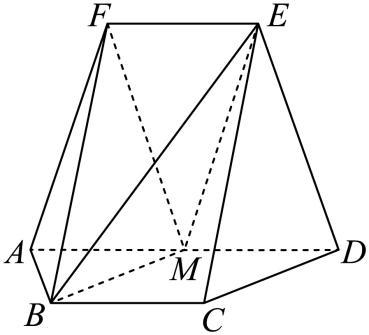
\includegraphics[width=.42\linewidth]{assets/asset-181-01.jpg}
\end{center}
\begin{solution}
\textbf{答案：}（1）证明见详解；（2）$\dfrac{4\sqrt{3}}{13}$

\textbf{分析：}（1）结合已知易证四边形 $BCDM$ 为平行四边形，可证 $BM\parallel CD$，进而得证；（2）作 $BO\perp AD$ 交 $AD$ 于 $O$，连接 $OF$，易证 $OB,OD,OF$ 三垂直，采用建系法结合二面角夹角余弦公式即可求解。

\textbf{详解：}（1）因为 $BC\parallel AD$，$EF=2$，$AD=4$，$M$ 为 $AD$ 的中点，所以 $BC\parallel MD$，$BC=MD$，四边形 $BCDM$ 为平行四边形，所以 $BM\parallel CD$，又因为 $BM\not\subset$ 平面 $CDE$，$CD\subset$ 平面 $CDE$，所以 $BM\parallel$ 平面 $CDE$。
（2）如图所示，作 $BO\perp AD$ 交 $AD$ 于 $O$，连接 $OF$，因为四边形 $ABCD$ 为等腰梯形，$BC\parallel AD$，$AD=4$，$AB=BC=2$，所以 $CD=2$，结合（1）$BCDM$ 为平行四边形，可得 $BM=CD=2$，又 $AM=2$，所以 $\triangle ABM$ 为等边三角形，$O$ 为 $AM$ 中点，所以 $OB=\sqrt{3}$，又因为四边形 $ADEF$ 为等腰梯形，$M$ 为 $AD$ 中点，所以 $EF=MD$，$EF\parallel MD$，四边形 $EFMD$ 为平行四边形，$FM=ED=AF$，所以 $\triangle AFM$ 为等腰三角形，$\triangle ABM$ 与 $\triangle AFM$ 底边上中点 $O$ 重合，$OF\perp AM$，$OF=\sqrt{AF^2-AO^2}=3$，因为 $OB^2+OF^2=BF^2$，所以 $OB\perp OF$，所以 $OB,OD,OF$ 互相垂直，以 $OB$ 方向为 $x$ 轴，$OD$ 方向为 $y$ 轴，$OF$ 方向为 $z$ 轴，建立 $O-xyz$ 空间直角坐标系，$F(0,0,3)$，$B(\sqrt{3},0,0)$，$M(0,1,0)$，$E(0,2,3)$，$\overrightarrow{BM}=(-\sqrt{3},1,0)$，$\overrightarrow{BF}=(-\sqrt{3},0,3)$，$\overrightarrow{BE}=(-\sqrt{3},2,3)$，设平面 $BFM$ 的法向量为 $\vec{m}=(x_1,y_1,z_1)$，平面 $EMB$ 的法向量为 $\vec{n}=(x_2,y_2,z_2)$，则 $\begin{cases} \vec{m}\cdot\overrightarrow{BM}=0 \\ \vec{m}\cdot\overrightarrow{BF}=0 \end{cases}$，即 $\begin{cases} -\sqrt{3}x_1+y_1=0 \\ -\sqrt{3}x_1+3z_1=0 \end{cases}$，令 $x_1=\sqrt{3}$，得 $y_1=3,z_1=1$，即 $\vec{m}=(\sqrt{3},3,1)$，$\begin{cases} \vec{n}\cdot\overrightarrow{BM}=0 \\ \vec{n}\cdot\overrightarrow{BE}=0 \end{cases}$，即 $\begin{cases} -\sqrt{3}x_2+y_2=0 \\ -\sqrt{3}x_2+2y_2+3z_2=0 \end{cases}$，令 $x_2=\sqrt{3}$，得 $y_2=3,z_2=-1$，即 $\vec{n}=(\sqrt{3},3,-1)$，$\cos\langle\vec{m},\vec{n}\rangle=\frac{\vec{m}\cdot\vec{n}}{|\vec{m}||\vec{n}|}=\frac{11}{\sqrt{13}\cdot\sqrt{13}}=\frac{11}{13}$，则 $\sin\langle\vec{m},\vec{n}\rangle=\frac{4\sqrt{3}}{13}$，故二面角 $F-BM-E$ 的正弦值为 $\frac{4\sqrt{3}}{13}$。
\end{solution}
\end{question}

\begin{question}[points=5]
\textbf{来源：}2024 年 全国甲卷-文科，第 10 题\par
设 $\alpha$、$\beta$ 是两个平面，$m$、$n$ 是两条直线，且 $\alpha \cap \beta = m$．下列四个命题：①若 $m // n$，则 $n // \alpha$ 或 $n // \beta$；②若 $m \perp n$，则 $n \perp \alpha$，$n \perp \beta$；③若 $n // \alpha$，且 $n // \beta$，则 $m // n$；④若 $n$ 与 $\alpha$ 和 $\beta$ 所成的角相等，则 $m \perp n$．其中所有真命题的编号是（ ）
\begin{choices}
  \item ①③
  \item ②④
  \item ①②③
  \item ①③④
\end{choices}
\begin{solution}
\textbf{答案：}A

\textbf{分析：}根据线面平行的判定定理即可判断①；举反例即可判断②④；根据线面平行的性质即可判断③.

\textbf{详解：}对①，当 $n \subset \alpha$，因为 $m // n$，$m \subset \beta$，则 $n // \beta$；当 $n \subset \beta$，因为 $m // n$，$m \subset \alpha$，则 $n // \alpha$；当 $n$ 既不在 $\alpha$ 也不在 $\beta$ 内，因为 $m // n$，$m \subset \alpha$，$m \subset \beta$，则 $n // \alpha$ 且 $n // \beta$，故①正确；对②，若 $m \perp n$，则 $n$ 与 $\alpha$，$\beta$ 不一定垂直，故②错误；对③，过直线 $n$ 分别作两平面与 $\alpha$，$\beta$ 分别相交于直线 $s$ 和直线 $t$，因为 $n // \alpha$，过直线 $n$ 的平面与平面 $\alpha$ 的交线为直线 $s$，则根据线面平行的性质定理知 $n // s$，同理可得 $n // t$，则 $s // t$，因为 $s \not\subset$ 平面 $\beta$，$t \subset$ 平面 $\beta$，则 $s //$ 平面 $\beta$，因为 $s \subset$ 平面 $\alpha$，$\alpha \cap \beta = m$，则 $s // m$，又因为 $n // s$，则 $m // n$，故③正确；对④，若 $\alpha \cap \beta = m$，$n$ 与 $\alpha$ 和 $\beta$ 所成的角相等，如果 $n // \alpha$，$n // \beta$，则 $m // n$，故④错误；综上只有①③正确.
\end{solution}
\end{question}

\begin{question}[points=12]
\textbf{来源：}2024 年 全国甲卷-文科，第 16 题\par
如图，在以 $A, B, C, D, E, F$ 为顶点的五面体中，四边形 $ABCD$ 与四边形 $ADEF$ 均为等腰梯形，$BC // AD$，$EF // AD$，$AD = 4$，$AB = BC = EF = 2$，$ED = \sqrt{10}$，$FB = 2\sqrt{3}$，$M$ 为 $AD$ 的中点．

（1）证明：$BM //$ 平面 $CDE$；

（2）求点 $M$ 到 $ABF$ 的距离．

\begin{center}
  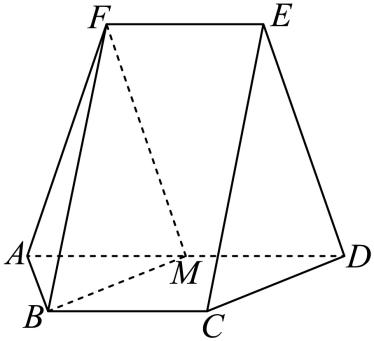
\includegraphics[width=.42\linewidth]{assets/asset-183-01.jpg}
\end{center}
\begin{solution}
\textbf{答案：}（1）证明见解析；（2）$\frac{3\sqrt{13}}{13}$

\textbf{分析：}（1）结合已知易证四边形 $BCDM$ 为平行四边形，可证 $BM // CD$，进而得证；（2）作 $FO \perp AD$，连接 $OB$，易证 $OB, OD, OF$ 三垂直，结合等体积法 $V_{M-ABF} = V_{F-ABM}$ 即可求解.

\textbf{详解：}（1）因为 $BC // AD$，$BC = 2$，$AD = 4$，$M$ 为 $AD$ 的中点，所以 $BC // MD$，$BC = MD$，四边形 $BCDM$ 为平行四边形，所以 $BM // CD$，又因为 $BM \not\subset$ 平面 $CDE$，$CD \subset$ 平面 $CDE$，所以 $BM //$ 平面 $CDE$．
（2）如图所示，作 $BO \perp AD$ 交 $AD$ 于 $O$，连接 $OF$，因为四边形 $ABCD$ 为等腰梯形，$BC // AD$，$AD = 4$，$AB = BC = 2$，所以 $CD = 2$，结合（1）$BCDM$ 为平行四边形，可得 $BM = CD = 2$，又 $AM = 2$，所以 $\triangle ABM$ 为等边三角形，$O$ 为 $AM$ 中点，所以 $OB = \sqrt{3}$，又因为四边形 $ADEF$ 为等腰梯形，$M$ 为 $AD$ 中点，所以 $EF = MD$，$EF // MD$，四边形 $EFMD$ 为平行四边形，$FM = ED = \sqrt{10} = AF$，所以 $\triangle AFM$ 为等腰三角形，$\triangle ABM$ 与 $\triangle AFM$ 底边上中点 $O$ 重合，$OF \perp AM$，$OF = \sqrt{AF^2 - AO^2} = \sqrt{10 - 1} = 3$，因为 $OB^2 + OF^2 = 3 + 9 = 12 = (2\sqrt{3})^2 = BF^2$，所以 $OB \perp OF$，所以 $OB, OD, OF$ 互相垂直，由等体积法可得 $V_{M-ABF} = V_{F-ABM}$，$V_{F-ABM} = \frac{1}{3} \cdot S_{\triangle ABM} \cdot FO = \frac{1}{3} \cdot \frac{1}{2} \cdot 2 \cdot \sqrt{3} \cdot 3 = \sqrt{3}$，在 $\triangle FAB$ 中，$FA = \sqrt{10}$，$AB = 2$，$FB = 2\sqrt{3}$，$\cos \angle FAB = \frac{FA^2 + AB^2 - FB^2}{2 \cdot FA \cdot AB} = \frac{10 + 4 - 12}{2 \cdot \sqrt{10} \cdot 2} = \frac{2}{4\sqrt{10}} = \frac{1}{2\sqrt{10}}$，$\sin \angle FAB = \sqrt{1 - \frac{1}{40}} = \sqrt{\frac{39}{40}} = \frac{\sqrt{39}}{2\sqrt{10}}$，$S_{\triangle FAB} = \frac{1}{2} \cdot FA \cdot AB \cdot \sin \angle FAB = \frac{1}{2} \cdot \sqrt{10} \cdot 2 \cdot \frac{\sqrt{39}}{2\sqrt{10}} = \frac{\sqrt{39}}{2}$，设点 $M$ 到 $FAB$ 的距离为 $d$，则 $V_{M-FAB} = V_{F-ABM} = \frac{1}{3} \cdot S_{\triangle FAB} \cdot d = \frac{1}{3} \cdot \frac{\sqrt{39}}{2} \cdot d = \sqrt{3}$，解得 $d = \frac{6\sqrt{3}}{\sqrt{39}} = \frac{6\sqrt{3} \cdot \sqrt{39}}{39} = \frac{6 \cdot 3\sqrt{13}}{39} = \frac{18\sqrt{13}}{39} = \frac{3\sqrt{13}}{13}$，即点 $M$ 到 $ABF$ 的距离为 $\frac{3\sqrt{13}}{13}$.
\end{solution}
\end{question}

\begin{question}[points=14]
\textbf{来源：}2024 年 上海卷，第 17 题\par
如图为正四棱锥$P-ABCD$，$O$为底面$ABCD$的中心．

\begin{center}
  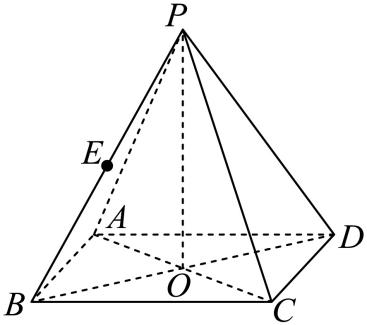
\includegraphics[width=.42\linewidth]{assets/asset-184-01.jpg}
\end{center}
\begin{solution}
\textbf{答案：}（1）$12\pi$；（2）$\frac{\pi}{4}$

\textbf{分析：}（1）根据正四棱锥的数据，先算出直角三角形$\triangle POA$的边长，然后求圆锥的体积；（2）连接$EA,EO,EC$，可先证$BE\perp$平面$ACE$，根据线面角的定义得出所求角为$\angle BOE$，然后结合题目数量关系求解.

\textbf{详解：}（1）正四棱锥满足且$PO\perp$平面$ABCD$，由$AO\subset$平面$ABCD$，则$PO\perp AO$，又正四棱锥底面$ABCD$是正方形，由$AD=3\sqrt2$可得，$AO=3$，故$PO=\sqrt{PA^2-AO^2}=4$，根据圆锥的定义，$\triangle POA$绕$PO$旋转一周形成的几何体是以$PO$为轴，$AO$为底面半径的圆锥，即圆锥的高为$PO=4$，底面半径为$AO=3$，根据圆锥的体积公式，所得圆锥的体积是$\frac13\times\pi\times3^2\times4=12\pi$.（2）连接$EA,EO,EC$，由题意结合正四棱锥的性质可知，每个侧面都是等边三角形，由$E$是$PB$中点，则$AE\perp PB$，$CE\perp PB$，又$AE\cap CE=E$，$AE,CE\subset$平面$ACE$，故$PB\perp$平面$ACE$，即$BE\perp$平面$ACE$，又$BD\cap$平面$ACE=O$，于是直线$BD$与平面$AEC$所成角的大小即为$\angle BOE$，不妨设$AP=AD=6$，则$BO=3\sqrt2$，$BE=3$，$\sin\angle BOE=\frac{3}{3\sqrt2}=\frac{\sqrt2}{2}$，又线面角的范围是$[0,\frac{\pi}{2}]$，故$\angle BOE=\frac{\pi}{4}$，即为所求.
\end{solution}
\end{question}

\begin{question}[points=5]
\textbf{来源：}2024 年 天津卷，第 6 题\par
若 $m,n$ 为两条不同的直线, $\alpha$ 为一个平面, 则下列结论中正确的是 ( )
\begin{choices}
  \item 若 $m // \alpha$, $n \subset \alpha$, 则 $m // n$
  \item 若 $m // \alpha$, $n // \alpha$, 则 $m // n$
  \item 若 $m // \alpha$, $n \perp \alpha$, 则 $m \perp n$
  \item 若 $m // \alpha$, $n \perp \alpha$, 则 $m$ 与 $n$ 相交
\end{choices}
\begin{solution}
\textbf{答案：}若 $m // \alpha$, $n \perp \alpha$, 则 $m \perp n$

\textbf{分析：}根据线面平行的性质可判断AB的正误，根据线面垂直的性质可判断CD的正误.

\textbf{详解：}对于A, 若 $m // \alpha$, $n \subset \alpha$, 则 $m,n$ 平行或异面, 故A错误. 对于B, 若 $m // \alpha$, $n // \alpha$, 则 $m,n$ 平行或异面或相交, 故B错误. 对于C, $m // \alpha$, $n \perp \alpha$, 过 $m$ 作平面 $\beta$, 使得 $\beta \cap \alpha = s$, 因为 $m \subset \beta$, 故 $m // s$, 而 $s \subset \alpha$, 故 $n \perp s$, 故 $m \perp n$, 故C正确. 对于D, 若 $m // \alpha$, $n \perp \alpha$, 则 $m$ 与 $n$ 相交或异面, 故D错误. 故选C.
\end{solution}
\end{question}

\begin{question}[points=5]
\textbf{来源：}2024 年 天津卷，第 9 题\par
一个五面体 $ABC-DEF$. 已知 $AD \parallel BE \parallel CF$, 且两两之间距离为 $1$. 并已知 $AD=1$, $BE=2$, $CF=3$. 则该五面体的体积为 ( )
\begin{choices}
  \item $\frac{\sqrt{3}}{6}$
  \item $\frac{3\sqrt{3}}{4}+\frac{1}{2}$
  \item $\frac{\sqrt{3}}{2}$
  \item $\frac{3\sqrt{3}}{4}-\frac{1}{2}$
\end{choices}
\begin{solution}
\textbf{答案：}$\frac{\sqrt{3}}{2}$

\textbf{分析：}采用补形法, 补成一个棱柱, 求出其直截面, 再利用体积公式即可.

\textbf{详解：}用一个完全相同的五面体 $HIJ-LMN$ (顶点与五面体 $ABC-DEF$ 一一对应) 与该五面体相嵌, 使得 $D,N$; $E,M$; $F,L$ 重合. 因为 $AD \parallel BE \parallel CF$, 且两两之间距离为 $1$, $AD=1$, $BE=2$, $CF=3$, 则形成的新组合体为一个三棱柱, 该三棱柱的直截面 (与侧棱垂直的截面) 为边长为 $1$ 的等边三角形, 侧棱长为 $1+3=2+2=3+1=4$, $V_{ABC-DEF}=\frac{1}{2}V_{ABC-HIJ}=\frac{1}{2}\times\frac{1}{2}\times 1\times 1\times \frac{\sqrt{3}}{2}\times 4=\frac{\sqrt{3}}{2}$. 故选C.
\end{solution}
\end{question}

\begin{question}[points=15]
\textbf{来源：}2024 年 天津卷，第 17 题\par
已知四棱柱 $ABCD-A_1B_1C_1D_1$ 中, 底面 $ABCD$ 为梯形, $AB//CD$, $A_1A\perp$ 平面 $ABCD$, $AD\perp AB$, 其中 $AB=AA_1=2$, $AD=DC=1$. $N$ 是 $B_1C_1$ 的中点, $M$ 是 $DD_1$ 的中点.

(1) 求证 $D_1N//$ 平面 $CB_1M$;

(2) 求平面 $CB_1M$ 与平面 $BB_1CC_1$ 的夹角余弦值;

(3) 求点 $B$ 到平面 $CB_1M$ 的距离.
\begin{solution}
\textbf{答案：}(1) 证明见解析; (2) $\frac{2\sqrt{22}}{11}$; (3) $\frac{2\sqrt{11}}{11}$

\textbf{分析：}(1) 取 $CB_1$ 中点 $P$, 连接 $NP$, $MP$, 借助中位线的性质与平行四边形性质定理可得 $D_1N//MP$, 结合线面平行判定定理即可得证. (2) 建立空间直角坐标系, 计算两平面的法向量, 再计算夹角余弦. (3) 利用点到平面的距离公式.

\textbf{详解：}(1) 取 $CB_1$ 中点 $P$, 连接 $NP$, $MP$. 由 $N$ 是 $B_1C_1$ 的中点, 故 $NP//CC_1$, 且 $NP=\frac{1}{2}CC_1$. 由 $M$ 是 $DD_1$ 的中点, 故 $D_1M=\frac{1}{2}DD_1=\frac{1}{2}CC_1$, 且 $D_1M//CC_1$, 则有 $D_1M//NP$, $D_1M=NP$, 故四边形 $D_1MPN$ 是平行四边形, 故 $D_1N//MP$. 又 $MP\subset$ 平面 $CB_1M$, $D_1N\not\subset$ 平面 $CB_1M$, 故 $D_1N//$ 平面 $CB_1M$.
(2) 以 $A$ 为原点建立空间直角坐标系, 有 $A(0,0,0)$, $B(2,0,0)$, $B_1(2,0,2)$, $M(0,1,1)$, $C(1,1,0)$, $C_1(1,1,2)$. 则 $\overrightarrow{CB_1}=(1,-1,2)$, $\overrightarrow{CM}=(-1,0,1)$, $\overrightarrow{BB_1}=(0,0,2)$. 设平面 $CB_1M$ 的法向量 $\vec{m}=(x_1,y_1,z_1)$, 由 $\begin{cases} \vec{m}\cdot\overrightarrow{CB_1}=x_1-y_1+2z_1=0\\ \vec{m}\cdot\overrightarrow{CM}=-x_1+z_1=0 \end{cases}$, 取 $x_1=1$, 则 $z_1=1$, $y_1=3$, 即 $\vec{m}=(1,3,1)$. 设平面 $BB_1CC_1$ 的法向量 $\vec{n}=(x_2,y_2,z_2)$, 由 $\begin{cases} \vec{n}\cdot\overrightarrow{CB_1}=x_2-y_2+2z_2=0\\ \vec{n}\cdot\overrightarrow{BB_1}=2z_2=0 \end{cases}$, 取 $x_2=1$, 则 $y_2=1$, $z_2=0$, 即 $\vec{n}=(1,1,0)$. 则 $\cos\langle\vec{m},\vec{n}\rangle=\frac{\vec{m}\cdot\vec{n}}{|\vec{m}||\vec{n}|}=\frac{1+3}{\sqrt{11}\cdot\sqrt{2}}=\frac{4}{\sqrt{22}}=\frac{2\sqrt{22}}{11}$. 故平面 $CB_1M$ 与平面 $BB_1CC_1$ 的夹角余弦值为 $\frac{2\sqrt{22}}{11}$.
(3) 由 $\overrightarrow{BB_1}=(0,0,2)$, 平面 $CB_1M$ 的法向量 $\vec{m}=(1,3,1)$, 则点 $B$ 到平面 $CB_1M$ 的距离 $d=\frac{|\overrightarrow{BB_1}\cdot\vec{m}|}{|\vec{m}|}=\frac{|2|}{\sqrt{11}}=\frac{2\sqrt{11}}{11}$.
\end{solution}
\end{question}

\begin{question}[points=5]
\textbf{来源：}2024 年 新高考II卷，第 7 题\par
已知正三棱台$ABC-A_1B_1C_1$的体积为$\dfrac{52}{3}$，$AB=6$，$A_1B_1=2$，则$A_1A$与平面$ABC$所成角的正切值为（ ）
\begin{choices}
  \item $\dfrac{1}{2}$
  \item $1$
  \item $2$
  \item $3$
\end{choices}
\begin{solution}
\textbf{答案：}$B$

\textbf{分析：}解法一：根据台体的体积公式可得三棱台的高$h=\dfrac{4\sqrt{3}}{3}$，做辅助线，结合正三棱台的结构特征求得$AM=\dfrac{4\sqrt{3}}{3}$，进而根据线面夹角的定义分析求解；解法二：将正三棱台$ABC-A_1B_1C_1$补成正三棱锥$P-ABC$，$A_1A$与平面$ABC$所成角即为$PA$与平面$ABC$所成角，根据比例关系可得$V_{P-ABC}=18$，进而可求正三棱锥$P-ABC$的高，即可得结果.

\textbf{详解：}解法一：分别取$BC,B_1C_1$的中点$D,D_1$，则$AD=3\sqrt{3}$，$A_1D_1=\sqrt{3}$。可知$S_{\triangle ABC}=\dfrac{1}{2}\times6\times6\times\dfrac{\sqrt{3}}{2}=9\sqrt{3}$，$S_{\triangle A_1B_1C_1}=\dfrac{1}{2}\times2\times\sqrt{3}=\sqrt{3}$。设正三棱台$ABC-A_1B_1C_1$的高为$h$，则$V_{ABC-A_1B_1C_1}=\dfrac{1}{3}(9\sqrt{3}+\sqrt{3}+\sqrt{9\sqrt{3}\times\sqrt{3}})h=\dfrac{52}{3}$，解得$h=\dfrac{4\sqrt{3}}{3}$。如图，分别过$A_1,D_1$作底面垂线，垂足为$M,N$，设$AM=x$，则$AA_1=\sqrt{AM^2+A_1M^2}=\sqrt{x^2+\dfrac{16}{3}}$，$DN=AD-AM-MN=2\sqrt{3}-x$，可得$DD_1=\sqrt{DN^2+D_1N^2}=\sqrt{(2\sqrt{3}-x)^2+\dfrac{16}{3}}$。结合等腰梯形$BCC_1B_1$可得$BB_1^2=\left(\dfrac{6-2}{2}\right)^2+DD_1^2$，即$x^2+\dfrac{16}{3}=(2\sqrt{3}-x)^2+\dfrac{16}{3}+4$，解得$x=\dfrac{4\sqrt{3}}{3}$。所以$A_1A$与平面$ABC$所成角的正切值为$\tan\angle A_1AD=\dfrac{A_1M}{AM}=1$。解法二：将正三棱台$ABC-A_1B_1C_1$补成正三棱锥$P-ABC$，则$A_1A$与平面$ABC$所成角即为$PA$与平面$ABC$所成角。因为$\dfrac{PA_1}{PA}=\dfrac{A_1B_1}{AB}=\dfrac{1}{3}$，则$\dfrac{V_{P-A_1B_1C_1}}{V_{P-ABC}}=\dfrac{1}{27}$，可知$V_{ABC-A_1B_1C_1}=\dfrac{26}{27}V_{P-ABC}=\dfrac{52}{3}$，则$V_{P-ABC}=18$。设正三棱锥$P-ABC$的高为$d$，则$V_{P-ABC}=\dfrac{1}{3}\times\dfrac{1}{2}\times6\times6\times\dfrac{\sqrt{3}}{2}\times d=18$，解得$d=2\sqrt{3}$。取底面$ABC$的中心为$O$，则$PO\perp$底面$ABC$，且$AO=2\sqrt{3}$，所以$PA$与平面$ABC$所成角的正切值$\tan\angle PAO=\dfrac{PO}{AO}=1$.
\end{solution}
\end{question}

\begin{question}[points=15]
\textbf{来源：}2024 年 新高考II卷，第 17 题\par
如图，平面四边形$ABCD$中，$AB=8$，$CD=3$，$AD=5\sqrt{3}$，$\angle ADC=90^\circ$，$\angle BAD=30^\circ$，点$E,F$满足$\overrightarrow{AE}=\dfrac{2}{5}\overrightarrow{AD}$，$\overrightarrow{AF}=\dfrac{1}{2}\overrightarrow{AB}$，将$\triangle AEF$沿$EF$对折至$\triangle PEF$，使得$PC=4\sqrt{3}$.

(1)证明：$EF\perp PD$；

(2)求面$PCD$与面$PBF$所成的二面角的正弦值.

\begin{center}
  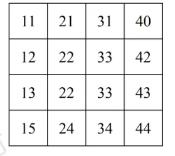
\includegraphics[width=.42\linewidth]{assets/asset-189-01.jpg}
\end{center}

\begin{center}
  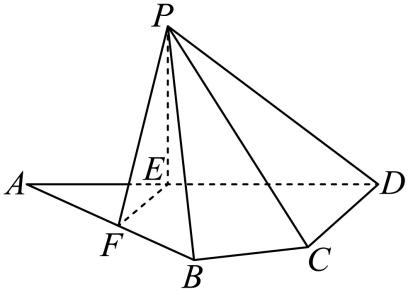
\includegraphics[width=.42\linewidth]{assets/asset-189-02.jpg}
\end{center}
\begin{solution}
\textbf{答案：}(1)证明见解析
(2)$\dfrac{8\sqrt{65}}{65}$

\textbf{分析：}(1)由题意，根据余弦定理求得$EF=2$，利用勾股定理的逆定理可证得$EF\perp AD$，则$EF\perp PE$，$EF\perp DE$，结合线面垂直的判定定理与性质即可证明；(2)由(1)，根据线面垂直的判定定理与性质可证明$PE\perp ED$，建立如图空间直角坐标系$E-xyz$，利用空间向量法求解面面角即可.

\textbf{详解：}（1）由$AB=8,AD=5\sqrt{3},\overrightarrow{AE}=\dfrac{2}{5}\overrightarrow{AD},\overrightarrow{AF}=\dfrac{1}{2}\overrightarrow{AB}$，得$AE=2\sqrt{3},AF=4$。又$\angle BAD=30^\circ$，在$\triangle AEF$中，由余弦定理得$EF=\sqrt{AE^2+AF^2-2AE\cdot AF\cos\angle BAD}=\sqrt{16+12-2\cdot4\cdot2\sqrt{3}\cdot\dfrac{\sqrt{3}}{2}}=2$，所以$AE^2+EF^2=AF^2$，则$AE\perp EF$，即$EF\perp AD$，所以$EF\perp PE$，$EF\perp DE$，又$PE\cap DE=E$，$PE,DE\subset$平面$PDE$，所以$EF\perp$平面$PDE$，又$PD\subset$平面$PDE$，故$EF\perp PD$。
（2）连接$CE$，由$\angle ADC=90^\circ,ED=3\sqrt{3},CD=3$，则$CE^2=ED^2+CD^2=36$。在$\triangle PEC$中，$PC=4\sqrt{3},PE=2\sqrt{3},EC=6$，得$EC^2+PE^2=PC^2$，所以$PE\perp EC$，由(1)知$PE\perp EF$，又$EC\cap EF=E$，$EC,EF\subset$平面$ABCD$，所以$PE\perp$平面$ABCD$，又$ED\subset$平面$ABCD$，所以$PE\perp ED$，则$PE,EF,ED$两两垂直，建立如图空间直角坐标系$E-xyz$，则$E(0,0,0)$，$P(0,0,2\sqrt{3})$，$D(0,3\sqrt{3},0)$，$C(3,3\sqrt{3},0)$，$F(2,0,0)$，$A(0,-2\sqrt{3},0)$，由$F$是$AB$的中点，得$B(4,2\sqrt{3},0)$。所以$\overrightarrow{PC}=(3,3\sqrt{3},-2\sqrt{3})$，$\overrightarrow{PD}=(0,3\sqrt{3},-2\sqrt{3})$，$\overrightarrow{PB}=(4,2\sqrt{3},-2\sqrt{3})$，$\overrightarrow{PF}=(2,0,-2\sqrt{3})$。设平面$PCD$和平面$PBF$的一个法向量分别为$\vec{n}=(x_1,y_1,z_1)$，$\vec{m}=(x_2,y_2,z_2)$，则$\begin{cases}\vec{n}\cdot\overrightarrow{PC}=3x_1+3\sqrt{3}y_1-2\sqrt{3}z_1=0\\\vec{n}\cdot\overrightarrow{PD}=3\sqrt{3}y_1-2\sqrt{3}z_1=0\end{cases}$，$\begin{cases}\vec{m}\cdot\overrightarrow{PB}=4x_2+2\sqrt{3}y_2-2\sqrt{3}z_2=0\\\vec{m}\cdot\overrightarrow{PF}=2x_2-2\sqrt{3}z_2=0\end{cases}$，令$y_1=2$，$x_2=\sqrt{3}$，得$x_1=0,z_1=3,y_2=-1,z_2=1$，所以$\vec{n}=(0,2,3)$，$\vec{m}=(\sqrt{3},-1,1)$，所以$\cos\langle\vec{m},\vec{n}\rangle=\dfrac{\vec{m}\cdot\vec{n}}{|\vec{m}||\vec{n}|}=\dfrac{1}{5\cdot\sqrt{13}}=\dfrac{\sqrt{65}}{65}$。设平面$PCD$和平面$PBF$所成角为$\theta$，则$\sin\theta=\sqrt{1-\cos^2\theta}=\dfrac{8\sqrt{65}}{65}$，即平面$PCD$和平面$PBF$所成角的正弦值为$\dfrac{8\sqrt{65}}{65}$.
\end{solution}
\end{question}

\begin{question}[points=5]
\textbf{来源：}2024 年 新高考I卷，第 5 题\par
已知圆柱和圆锥的底面半径相等，侧面积相等，且它们的高均为 $\sqrt{3}$，则圆锥的体积为（ ）
\begin{choices}
  \item $2\sqrt{3}\pi$
  \item $3\sqrt{3}\pi$
  \item $6\sqrt{3}\pi$
  \item $9\sqrt{3}\pi$
\end{choices}
\begin{solution}
\textbf{答案：}B

\textbf{分析：}设圆柱的底面半径为 $r$，根据圆锥和圆柱的侧面积相等可得半径 $r$ 的方程，求出解后可求圆锥的体积.

\textbf{详解：}设圆柱的底面半径为 $r$，则圆锥的母线长为 $\sqrt{r^2+3}$，而它们的侧面积相等，所以 $2\pi r\times\sqrt{3}=\pi r\times\sqrt{3+r^2}$，即 $2\sqrt{3}=\sqrt{3+r^2}$，故 $r=3$，故圆锥的体积为 $\dfrac{1}{3}\pi\times 9\times\sqrt{3}=3\sqrt{3}\pi$.
\end{solution}
\end{question}

\begin{question}[points=15]
\textbf{来源：}2024 年 新高考I卷，第 17 题\par
如图，四棱锥 $P-ABCD$ 中，$PA\perp$ 底面 $ABCD$，$PA=AC=2$，$BC=1, AB=\sqrt{3}$.

(1) 若 $AD\perp PB$，证明：$AD\parallel$ 平面 $PBC$；

(2) 若 $AD\perp DC$，且二面角 $A-CP-D$ 的正弦值为 $\dfrac{\sqrt{42}}{7}$，求 $AD$.
\begin{solution}
\textbf{答案：}(1) 证明见解析 (2) $AD=\sqrt{3}$

\textbf{分析：}(1) 先证出 $AD\perp$ 平面 $PAB$，即可得 $AD\perp AB$，由勾股定理逆定理可得 $BC\perp AB$，从而 $AD\parallel BC$，再根据线面平行的判定定理即可证出；(2) 过点 $D$ 作 $DE\perp AC$ 于 $E$，再过点 $E$ 作 $EF\perp CP$ 于 $F$，连接 $DF$，根据三垂线法可知，$\angle DFE$ 即为二面角 $A-CP-D$ 的平面角，即可求得 $\tan\angle DFE=\sqrt{6}$，再分别用 $AD$ 的长度表示出 $DE,EF$，即可解方程求出 $AD$.

\textbf{详解：}(1) 因为 $PA\perp$ 平面 $ABCD$，$AD\subset$ 平面 $ABCD$，所以 $PA\perp AD$，又 $AD\perp PB$，$PB\cap PA=P$，$PB,PA\subset$ 平面 $PAB$，所以 $AD\perp$ 平面 $PAB$，而 $AB\subset$ 平面 $PAB$，所以 $AD\perp AB$. 因为 $BC^2+AB^2=1+3=4=AC^2$，所以 $BC\perp AB$，根据平面知识可知 $AD\parallel BC$，又 $AD\not\subset$ 平面 $PBC$，$BC\subset$ 平面 $PBC$，所以 $AD\parallel$ 平面 $PBC$.
(2) 如图所示，过点 $D$ 作 $DE\perp AC$ 于 $E$，再过点 $E$ 作 $EF\perp CP$ 于 $F$，连接 $DF$，因为 $PA\perp$ 平面 $ABCD$，所以平面 $PAC\perp$ 平面 $ABCD$，而平面 $PAC\cap$ 平面 $ABCD=AC$，所以 $DE\perp$ 平面 $PAC$，又 $EF\perp CP$，所以 $CP\perp$ 平面 $DEF$，根据二面角的定义可知，$\angle DFE$ 即为二面角 $A-CP-D$ 的平面角，即 $\sin\angle DFE=\dfrac{\sqrt{42}}{7}$，即 $\tan\angle DFE=\sqrt{6}$. 因为 $AD\perp DC$，设 $AD=x$，则 $CD=\sqrt{4-x^2}$，由等面积法可得，$DE=\dfrac{x\sqrt{4-x^2}}{2}$，又 $CE=\sqrt{(4-x^2)-\left(\dfrac{x\sqrt{4-x^2}}{2}\right)^2}=\dfrac{4-x^2}{2}$，而 $\triangle EFC$ 为等腰直角三角形，所以 $EF=\dfrac{\sqrt{2}}{2}CE=\dfrac{\sqrt{2}}{2}\cdot\dfrac{4-x^2}{2}=\dfrac{\sqrt{2}(4-x^2)}{4}$，故 $\tan\angle DFE=\dfrac{DE}{EF}=\dfrac{\frac{x\sqrt{4-x^2}}{2}}{\frac{\sqrt{2}(4-x^2)}{4}}=\dfrac{\sqrt{2}x}{\sqrt{4-x^2}}=\sqrt{6}$，解得 $x=\sqrt{3}$，即 $AD=\sqrt{3}$.
\end{solution}
\end{question}

\section*{2025 年}

\begin{question}[points=5]
\textbf{来源：}2025 年 全国II卷，第 14 题\par
一个底面半径为 $4\mathrm{cm}$，高为 $9\mathrm{cm}$ 的封闭圆柱形容器（容器壁厚度忽略不计）内有两个半径相等的铁球，则铁球半径的最大值为 $\mathrm{cm}$.
\fillin[{$\frac{5}{2}$}]
\begin{solution}
\textbf{答案：}$\frac{5}{2}$

\textbf{分析：}根据圆柱与球的性质以及球的体积公式可求出球的半径.

\textbf{详解：}圆柱的底面半径为 $4\mathrm{cm}$，设铁球的半径为 $r$，且 $r<4$，由圆柱与球的性质知 $AB^2=(2r)^2=(8-2r)^2+(9-2r)^2$，即 $4r^2-68r+145=(2r-5)(2r-29)=0$，因为 $r<4$，所以 $r=\frac{5}{2}$.
\end{solution}
\end{question}

\begin{question}[points=15]
\textbf{来源：}2025 年 全国II卷，第 17 题\par
如图，在四边形 $ABCD$ 中，$AB\parallel CD$，$\angle DAB=90^\circ$，$F$ 为 $CD$ 的中点，点 $E$ 在 $AB$ 上，$EF\parallel AD$，$AB=3AD$，$CD=2AD$，将四边形 $EFDA$ 沿 $EF$ 翻折至四边形 $EFD'A'$，使得面 $EFD'A'$ 与面 $EFCB$ 所成的二面角为 $60^\circ$.

（1）证明: $A'B\parallel$ 平面 $CD'F$；

（2）求面 $BCD'$ 与面 $EFD'A'$ 所成的二面角的正弦值.

\begin{center}
  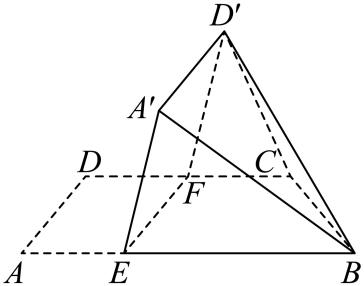
\includegraphics[width=.42\linewidth]{assets/asset-193-01.jpg}
\end{center}
\begin{solution}
\textbf{答案：}（1）证明见解析
（2）$\frac{\sqrt{42}}{7}$

\textbf{分析：}（1）先应用线面平行判定定理得出 $A'E\parallel$ 平面 $CD'F$ 及 $EB\parallel$ 平面 $CD'F$，再应用面面平行判定定理得出平面 $A'EB\parallel$ 平面 $CD'F$，进而得出线面平行；（2）建立空间直角坐标系，利用已知条件将点 $B,C,D',E,F$ 的坐标表示出来，然后将平面 $BCD'$ 及平面 $EFD'A'$ 的法向量求出来，利用两个法向量的数量积公式可将两平面的夹角余弦值求出来，进而可求得其正弦值.

\textbf{详解：}（1）设 $AD=1$，所以 $AB=3$，$CD=2$，因为 $F$ 为 $CD$ 中点，所以 $DF=1$，因为 $EF\parallel AD$，$AB\parallel CD$，所以 $AEFD$ 是平行四边形，所以 $AE\parallel DF$，所以 $A'E\parallel D'F$，因为 $D'F\subset$ 平面 $CD'F$，$A'E\not\subset$ 平面 $CD'F$，所以 $A'E\parallel$ 平面 $CD'F$，因为 $FC\parallel EB$，$FC\subset$ 平面 $CD'F$，$EB\not\subset$ 平面 $CD'F$，所以 $EB\parallel$ 平面 $CD'F$，又 $EB\cap A'E=E$，$EB,A'E\subset$ 平面 $A'EB$，所以平面 $A'EB\parallel$ 平面 $CD'F$，又 $A'B\subset$ 平面 $A'EB$，所以 $A'B\parallel$ 平面 $CD'F$.
（2）因为 $\angle DAB=90^\circ$，所以 $AD\perp AB$，又因为 $AB\parallel FC$，$EF\parallel AD$，所以 $EF\perp FC$，以 $F$ 为原点，$FE$，$FC$ 以及垂直于平面 $BECF$ 的直线分别为 $x$，$y$，$z$ 轴，建立空间直角坐标系. 因为 $D'F\perp EF$，$CF\perp EF$，平面 $EFD'A'$ 与平面 $EFCB$ 所成二面角为 $60^\circ$，所以 $\angle D'FC=60^\circ$. 则 $B(1,2,0)$，$C(0,1,0)$，$D'\left(0,\frac{1}{2},\frac{\sqrt{3}}{2}\right)$，$E(1,0,0)$，$F(0,0,0)$. 所以 $\overrightarrow{BC}=(-1,-1,0)$，$\overrightarrow{CD'}=\left(0,-\frac{1}{2},\frac{\sqrt{3}}{2}\right)$，$\overrightarrow{FE}=(1,0,0)$，$\overrightarrow{FD'}=\left(0,\frac{1}{2},\frac{\sqrt{3}}{2}\right)$. 设平面 $BCD'$ 的法向量为 $\vec{n}=(x,y,z)$，则 $\begin{cases}\overrightarrow{BC}\cdot\vec{n}=0\\\overrightarrow{CD'}\cdot\vec{n}=0\end{cases}$，即 $\begin{cases}-x-y=0\\-\frac{1}{2}y+\frac{\sqrt{3}}{2}z=0\end{cases}$，令 $y=\sqrt{3}$，则 $z=1$，$x=-\sqrt{3}$，则 $\vec{n}=(-\sqrt{3},\sqrt{3},1)$. 设平面 $EFD'A'$ 的法向量为 $\vec{m}=(x_1,y_1,z_1)$，则 $\begin{cases}\overrightarrow{FE}\cdot\vec{m}=0\\\overrightarrow{FD'}\cdot\vec{m}=0\end{cases}$，即 $\begin{cases}x_1=0\\\frac{1}{2}y_1+\frac{\sqrt{3}}{2}z_1=0\end{cases}$，令 $y_1=\sqrt{3}$，则 $z_1=-1$，$x_1=0$，所以 $\vec{m}=(0,\sqrt{3},-1)$. 所以 $\cos\langle\vec{m},\vec{n}\rangle=\frac{\vec{m}\cdot\vec{n}}{|\vec{m}||\vec{n}|}=\frac{0+3-1}{\sqrt{3+3+1}\times\sqrt{1+3}}=\frac{1}{\sqrt{7}}$，所以平面 $BCD'$ 与平面 $EFD'A'$ 夹角的正弦值为 $\sqrt{1-\left(\frac{1}{\sqrt{7}}\right)^2}=\frac{\sqrt{42}}{7}$.
\end{solution}
\end{question}

\begin{question}[points=6]
\textbf{来源：}2025 年 全国I卷，第 9 题\par
在正三棱柱 $ABC-A_1B_1C_1$ 中，$D$ 为 $BC$ 中点，则（ ）

\begin{center}
  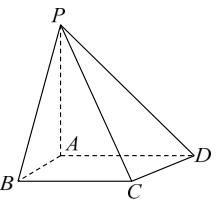
\includegraphics[width=.42\linewidth]{assets/asset-194-01.jpg}
\end{center}
\begin{choices}
  \item $AD \perp A_1C$
  \item $BC \perp$ 平面 $AA_1D$
  \item $CC_1 \parallel$ 平面 $AA_1D$
  \item $AD \parallel A_1B_1$
\end{choices}
\begin{solution}
\textbf{答案：}BC

\textbf{分析：}法一：对于 A，利用空间向量的线性运算与数量积运算即可判断；对于 B，利用线面垂直的判定与性质定理即可判断；对于 C，利用线面平行的判定定理即可判断；对于 D，利用反证法即可判断；法二：根据题意建立空间直角坐标系，利用空间向量法逐一分析判断各选项即可得解.

\textbf{详解：}法一：对于 A，$A_1C \cdot AD = (A_1A + AD + CD) \cdot AD = A_1A \cdot AD + AD^2 + CD \cdot AD = AD^2 \neq 0$，则 $AD \perp A_1C$ 不成立，故 A 错误；对于 B，$AA_1 \perp BC$，$AD \perp BC$，且 $AA_1 \cap AD = A$，所以 $BC \perp$ 平面 $AA_1D$，故 B 正确；对于 C，$CC_1 \parallel AA_1$，$AA_1 \subset$ 平面 $AA_1D$，$CC_1 \not\subset$ 平面 $AA_1D$，所以 $CC_1 \parallel$ 平面 $AA_1D$，故 C 正确；对于 D，$A_1B_1 \parallel AB$，假设 $AD \parallel A_1B_1$，则 $AD \parallel AB$，矛盾，故 D 错误. 故选：BC. 法二：略.
\end{solution}
\end{question}

\begin{question}[points=15]
\textbf{来源：}2025 年 全国I卷，第 17 题\par
如图所示的四棱锥 $P-ABCD$ 中，$PA \perp$ 平面 $ABCD$，$BC \parallel AD$，$AB \perp AD$.



（1）证明：平面 $PAB \perp$ 平面 $PAD$；



（2）$PA = AB = \sqrt{2}$，$AD = 1+\sqrt{3}$，$BC = 2$，$P$，$B$，$C$，$D$ 在同一个球面上，设该球面的球心为 $O$.



（i）证明：$O$ 在平面 $ABCD$ 上；



（ⅱ）求直线 $AC$ 与直线 $PO$ 所成角的余弦值.
\begin{solution}
\textbf{答案：}（1）证明见解析；（2）（i）证明见解析；（ii）$\frac{2}{3}$

\textbf{分析：}（1）通过证明 $AP \perp AB$，$AP \perp AD$，得出 $AB \perp$ 平面 $PAD$，即可证明面面垂直；（2）（i）法一：建立空间直角坐标系并表达出各点的坐标，假设 $P,B,C,D$ 在同一球面 $O$ 上，得出点 $O$ 坐标，即可证明结论；法二：作出 $\triangle BCD$ 的边 $BC$ 和 $CD$ 的垂直平分线，找到三角形的外心 $O_1$，求出 $PO_1$，得出外心 $O_1$ 即为球心，即可证明结论；（ii）法一：写出直线 $AC$ 和 $PO$ 的方向向量，即可求出余弦值；法二：求出 $AC$ 的长，过点 $O$ 作 $AC$ 的平行线，在 $\triangle POC_1$ 中由余弦定理求解.

\textbf{详解：}（1）因为 $PA \perp$ 平面 $ABCD$，$AB \subset$ 平面 $ABCD$，$AD \subset$ 平面 $ABCD$，所以 $PA \perp AB$，$PA \perp AD$，又 $AB \perp AD$，$PA \cap AD = A$，所以 $AB \perp$ 平面 $PAD$，而 $AB \subset$ 平面 $PAB$，故平面 $PAB \perp$ 平面 $PAD$.
（2）（i）法一：以 $A$ 为原点，$AB$ 为 $x$ 轴，$AD$ 为 $y$ 轴，$AP$ 为 $z$ 轴建立空间直角坐标系，则 $A(0,0,0)$，$B(\sqrt{2},0,0)$，$C(\sqrt{2},2,0)$，$D(0,1+\sqrt{3},0)$，$P(0,0,\sqrt{2})$，设 $O(x,y,z)$，由 $OP=OB=OC=OD$ 可解得 $x=0$，$y=1$，$z=0$，即 $O(0,1,0)$，显然在平面 $ABCD$ 上.
（ii）$\overrightarrow{AC} = (\sqrt{2},2,0)$，$\overrightarrow{PO} = (0,1,-\sqrt{2})$，设直线 $AC$ 与 $PO$ 所成角为 $\theta$，则 $\cos\theta = \frac{|\overrightarrow{AC} \cdot \overrightarrow{PO}|}{|\overrightarrow{AC}| |\overrightarrow{PO}|} = \frac{|0+2+0|}{\sqrt{(\sqrt{2})^2+2^2} \cdot \sqrt{0^2+1^2+(-\sqrt{2})^2}} = \frac{2}{\sqrt{6} \cdot \sqrt{3}} = \frac{2}{3}$.
\end{solution}
\end{question}

\begin{question}[points=5]
\textbf{来源：}2025 年 上海卷，第 7 题\par
如图，在正四棱柱 $ABCD-A_1B_1C_1D_1$ 中，$BD = 4\sqrt{2}, DB_1 = 9$，则该正四棱柱的体积为．

\begin{center}
  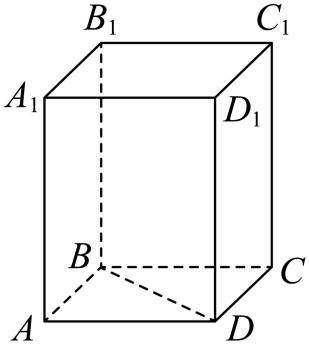
\includegraphics[width=.42\linewidth]{assets/asset-196-01.jpg}
\end{center}
\fillin[{$112$}]
\begin{solution}
\textbf{答案：}$112$

\textbf{分析：}求出侧棱长和底面边长后可求体积.

\textbf{详解：}因为 $BD = 4\sqrt{2}$ 且四边形 $ABCD$ 为正方形，故 $BA = 4$，而 $DB_1 = 9$，故 $BB_1^2 + BD^2 = 81$，故 $BB_1 = 7$，故所求体积为 $7 \times 16 = 112$ .
\end{solution}
\end{question}

\begin{question}[points=14]
\textbf{来源：}2025 年 上海卷，第 18 题\par
如图，$P$ 是圆锥的顶点，$O$ 是底面圆心，$AB$ 是底面直径，且 $AB = 2$．



(1) 若直线 $PA$ 与圆锥底面的所成角为 $\frac{\pi}{3}$，求圆锥的侧面积；

(2) 已知 $Q$ 是母线 $PA$ 的中点，点 $C$、$D$ 在底面圆周上，且弧 $AC$ 的长为 $\frac{\pi}{3}$，$CD \parallel AB$．设点 $M$ 在线段 $OC$ 上，证明：直线 $QM \parallel$ 平面 $PBD$．

\begin{center}
  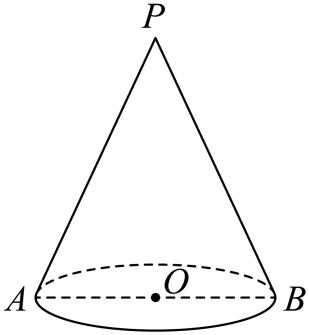
\includegraphics[width=.42\linewidth]{assets/asset-197-01.jpg}
\end{center}
\begin{solution}
\textbf{答案：}(1) $2\pi$； (2) 证明见解析

\textbf{分析：}(1) 由线面角先算出母线长，然后根据侧面积公式求解； (2) 证明平面 $QOC \parallel$ 平面 $PBD$，然后根据面面平行的性质可得.

\textbf{详解：}(1) 由题知，$\angle PAB = \frac{\pi}{3}$，即轴截面 $\triangle ABP$ 是等边三角形，故 $PA = AB = 2$，底面周长为 $2\pi \times 1 = 2\pi$，则侧面积为：$\frac{1}{2} \times 2 \times 2\pi = 2\pi$．
(2) 由题知 $AQ = QP, AO = OB$，则根据中位线性质，$QO \parallel PB$，又 $QO \not\subset$ 平面 $PBD$，$PB \subset$ 平面 $PBD$，则 $QO \parallel$ 平面 $PBD$．由于 $\widehat{AC} = \frac{\pi}{3}$，底面圆半径是 $1$，则 $\angle AOC = \frac{\pi}{3}$，又 $CD \parallel AB$，则 $\angle OCD = \frac{\pi}{3}$，又 $OC = OD$，则 $\triangle OCD$ 为等边三角形，则 $CD = 1$，于是 $CD \parallel BO$ 且 $CD = OB$，则四边形 $OBDC$ 是平行四边形，故 $OC \parallel BD$，又 $OC \not\subset$ 平面 $PBD$，$BD \subset$ 平面 $PBD$，故 $OC \parallel$ 平面 $PBD$．又 $OC \cap OQ = O$，$OC, OQ \subset$ 平面 $QOC$，根据面面平行的判定，于是平面 $QOC \parallel$ 平面 $PBD$，又 $M \in OC$，则 $QM \subset$ 平面 $QOC$，则 $QM \parallel$ 平面 $PBD$．
\end{solution}
\end{question}

\begin{question}[points=5]
\textbf{来源：}2025 年 天津卷，第 4 题\par
若$m$为直线，$\alpha, \beta$为两个平面，则下列结论中正确的是（   ）
\begin{choices}
  \item 若$m // \alpha$, $n \subset \alpha$, 则$m // n$
  \item 若$m \perp \alpha$, $m \perp \beta$, 则$\alpha \perp \beta$
  \item 若$m // \alpha$, $m \perp \beta$, 则$\alpha \perp \beta$
  \item 若$m \subset \alpha$, $\alpha \perp \beta$, 则$m \perp \beta$
\end{choices}
\begin{solution}
\textbf{答案：}C

\textbf{分析：}根据线面平行的定义可判断A的正误，根据空间中垂直关系的转化可判断BCD的正误.

\textbf{详解：}对于A，若$m // \alpha$, $n \subset \alpha$, 则$m, n$可平行或异面，故A错误；对于B，若$m \perp \alpha$, $m \perp \beta$, 则$\alpha // \beta$, 故B错误；对于C，两条平行线有一条垂直于一个平面，则另一个必定垂直这个平面，现$m // a$, $m \perp \beta$, 故$a \perp \beta$, 故C正确；对于D，$m \subset \alpha$, $\alpha \perp \beta$, 则$m$与$\beta$可平行或相交或$m \subset \beta$, 故D错误. 故选C.
\end{solution}
\end{question}

\begin{question}[points=15]
\textbf{来源：}2025 年 天津卷，第 17 题\par
正方体$ABCD - A_1B_1C_1D_1$的棱长为4, $E$、$F$分别为$A_1D_1$, $C_1B_1$中点, $CG = 3GC_1$.

(1) 求证: $GF \perp$平面$FBE$;

(2) 求平面$FBE$与平面$EBG$夹角的余弦值;

(3) 求三棱锥$D - FBE$的体积.
\begin{solution}

\textbf{分析：}(1)法一、利用正方形的性质先证明$FG \perp BF$, 再结合正方体的性质得出$EF \perp$平面$BCC_1B_1$, 利用线面垂直的性质与判定定理证明即可；法二、建立空间直角坐标系, 利用空间向量证明线面垂直即可；(2)利用空间向量计算面面夹角即可；(3)利用空间向量计算点面距离，再利用锥体的体积公式计算即可.

\textbf{详解：}（1）法一、在正方形$BCC_1B_1$中，由条件易知$\tan\angle C_1FG = \dfrac{C_1G}{C_1F} = \dfrac{1}{2} = \dfrac{FB_1}{BB_1} = \tan\angle B_1BF$，所以$\angle C_1FG = \angle B_1BF$，则$\angle B_1FB + \angle B_1BF = \dfrac{\pi}{2} = \angle C_1FG + \angle B_1FB$，故$\angle BFG = \pi - (\angle C_1FG + \angle B_1FB) = \dfrac{\pi}{2}$，即$FG \perp BF$. 在正方体中，易知$D_1C_1 \perp$平面$BCC_1B_1$，且$EF // D_1C_1$，所以$EF \perp$平面$BCC_1B_1$，又$FG \subset$平面$BCC_1B_1$，所以$EF \perp FG$. 因为$EF \cap BF = F$, $EF, BF \subset$平面$BEF$，所以$GF \perp$平面$BEF$.
法二、如图以$D$为中心建立空间直角坐标系，则$B(4,4,0)$, $E(2,0,4)$, $F(2,4,4)$, $G(0,4,3)$, 所以$\overrightarrow{EF} = (0,4,0)$, $\overrightarrow{EB} = (2,4,-4)$, $\overrightarrow{FG} = (-2,0,-1)$. 设$\vec{m} = (a,b,c)$是平面$BEF$的一个法向量，则$\begin{cases} \vec{m} \cdot \overrightarrow{EF} = 4b = 0 \\ \vec{m} \cdot \overrightarrow{EB} = 2a + 4b - 4c = 0 \end{cases}$, 令$a=2$, 则$b=0$, $c=1$, 所以$\vec{m} = (2,0,1)$. 易知$\overrightarrow{FG} = -\vec{m}$, 则$\overrightarrow{FG}$也是平面$BEF$的一个法向量，所以$GF \perp$平面$BEF$.
（2）同上法二建立的空间直角坐标系，所以$\overrightarrow{EG} = (-2,4,-1)$, $\overrightarrow{BG} = (-4,0,3)$. 由(1)知$\overrightarrow{FG}$是平面$BEF$的一个法向量. 设平面$BEG$的一个法向量为$\vec{n} = (x,y,z)$, 所以$\begin{cases} \vec{n} \cdot \overrightarrow{EG} = -2x + 4y - z = 0 \\ \vec{n} \cdot \overrightarrow{BG} = -4x + 3z = 0 \end{cases}$, 令$x=6$, 则$z=8$, $y=5$, 即$\vec{n} = (6,5,8)$. 设平面$BEF$与平面$BEG$的夹角为$\alpha$, 则$\cos\alpha = |\cos\langle\overrightarrow{FG},\vec{n}\rangle| = \dfrac{|\overrightarrow{FG}\cdot\vec{n}|}{|\overrightarrow{FG}||\vec{n}|} = \dfrac{20}{\sqrt{5} \times 5\sqrt{5}} = \dfrac{4}{5}$.
（3）由(1)知$EF \perp$平面$BCC_1B_1$, $FB \subset$平面$BCC_1B_1$, 所以$EF \perp FB$. 易知$S_{\triangle BEF} = \dfrac{1}{2} EF \cdot BF = \dfrac{1}{2} \times 4 \times \sqrt{4^2 + 2^2} = 4\sqrt{5}$. 又$\overrightarrow{DE} = (2,0,4)$, 则$D$到平面$BEF$的距离为$d = \dfrac{|\overrightarrow{DE} \cdot \overrightarrow{FG}|}{|\overrightarrow{FG}|} = \dfrac{8}{\sqrt{5}}$. 由棱锥的体积公式知：$V_{D-BEF} = \dfrac{1}{3} d \times S_{\triangle BEF} = \dfrac{1}{3} \times \dfrac{8}{\sqrt{5}} \times 4\sqrt{5} = \dfrac{32}{3}$.
\end{solution}
\end{question}

